% Options for packages loaded elsewhere
\PassOptionsToPackage{unicode}{hyperref}
\PassOptionsToPackage{hyphens}{url}
%
\documentclass[
]{book}
\usepackage{amsmath,amssymb}
\usepackage{lmodern}
\usepackage{ifxetex,ifluatex}
\ifnum 0\ifxetex 1\fi\ifluatex 1\fi=0 % if pdftex
  \usepackage[T1]{fontenc}
  \usepackage[utf8]{inputenc}
  \usepackage{textcomp} % provide euro and other symbols
\else % if luatex or xetex
  \usepackage{unicode-math}
  \defaultfontfeatures{Scale=MatchLowercase}
  \defaultfontfeatures[\rmfamily]{Ligatures=TeX,Scale=1}
\fi
% Use upquote if available, for straight quotes in verbatim environments
\IfFileExists{upquote.sty}{\usepackage{upquote}}{}
\IfFileExists{microtype.sty}{% use microtype if available
  \usepackage[]{microtype}
  \UseMicrotypeSet[protrusion]{basicmath} % disable protrusion for tt fonts
}{}
\makeatletter
\@ifundefined{KOMAClassName}{% if non-KOMA class
  \IfFileExists{parskip.sty}{%
    \usepackage{parskip}
  }{% else
    \setlength{\parindent}{0pt}
    \setlength{\parskip}{6pt plus 2pt minus 1pt}}
}{% if KOMA class
  \KOMAoptions{parskip=half}}
\makeatother
\usepackage{xcolor}
\IfFileExists{xurl.sty}{\usepackage{xurl}}{} % add URL line breaks if available
\IfFileExists{bookmark.sty}{\usepackage{bookmark}}{\usepackage{hyperref}}
\hypersetup{
  pdftitle={Tutorial for R microeco package (v0.5.0)},
  pdfauthor={Chi Liu, Umer Zeeshan Ijaz, Felipe Mansoldo, Chenhao Li, Yang Cao, Jarrod J. Scott, Yaoming Cui, Alane B. Vermelho, Xiangzhen Li, Minjie Yao},
  hidelinks,
  pdfcreator={LaTeX via pandoc}}
\urlstyle{same} % disable monospaced font for URLs
\usepackage{color}
\usepackage{fancyvrb}
\newcommand{\VerbBar}{|}
\newcommand{\VERB}{\Verb[commandchars=\\\{\}]}
\DefineVerbatimEnvironment{Highlighting}{Verbatim}{commandchars=\\\{\}}
% Add ',fontsize=\small' for more characters per line
\usepackage{framed}
\definecolor{shadecolor}{RGB}{248,248,248}
\newenvironment{Shaded}{\begin{snugshade}}{\end{snugshade}}
\newcommand{\AlertTok}[1]{\textcolor[rgb]{0.94,0.16,0.16}{#1}}
\newcommand{\AnnotationTok}[1]{\textcolor[rgb]{0.56,0.35,0.01}{\textbf{\textit{#1}}}}
\newcommand{\AttributeTok}[1]{\textcolor[rgb]{0.77,0.63,0.00}{#1}}
\newcommand{\BaseNTok}[1]{\textcolor[rgb]{0.00,0.00,0.81}{#1}}
\newcommand{\BuiltInTok}[1]{#1}
\newcommand{\CharTok}[1]{\textcolor[rgb]{0.31,0.60,0.02}{#1}}
\newcommand{\CommentTok}[1]{\textcolor[rgb]{0.56,0.35,0.01}{\textit{#1}}}
\newcommand{\CommentVarTok}[1]{\textcolor[rgb]{0.56,0.35,0.01}{\textbf{\textit{#1}}}}
\newcommand{\ConstantTok}[1]{\textcolor[rgb]{0.00,0.00,0.00}{#1}}
\newcommand{\ControlFlowTok}[1]{\textcolor[rgb]{0.13,0.29,0.53}{\textbf{#1}}}
\newcommand{\DataTypeTok}[1]{\textcolor[rgb]{0.13,0.29,0.53}{#1}}
\newcommand{\DecValTok}[1]{\textcolor[rgb]{0.00,0.00,0.81}{#1}}
\newcommand{\DocumentationTok}[1]{\textcolor[rgb]{0.56,0.35,0.01}{\textbf{\textit{#1}}}}
\newcommand{\ErrorTok}[1]{\textcolor[rgb]{0.64,0.00,0.00}{\textbf{#1}}}
\newcommand{\ExtensionTok}[1]{#1}
\newcommand{\FloatTok}[1]{\textcolor[rgb]{0.00,0.00,0.81}{#1}}
\newcommand{\FunctionTok}[1]{\textcolor[rgb]{0.00,0.00,0.00}{#1}}
\newcommand{\ImportTok}[1]{#1}
\newcommand{\InformationTok}[1]{\textcolor[rgb]{0.56,0.35,0.01}{\textbf{\textit{#1}}}}
\newcommand{\KeywordTok}[1]{\textcolor[rgb]{0.13,0.29,0.53}{\textbf{#1}}}
\newcommand{\NormalTok}[1]{#1}
\newcommand{\OperatorTok}[1]{\textcolor[rgb]{0.81,0.36,0.00}{\textbf{#1}}}
\newcommand{\OtherTok}[1]{\textcolor[rgb]{0.56,0.35,0.01}{#1}}
\newcommand{\PreprocessorTok}[1]{\textcolor[rgb]{0.56,0.35,0.01}{\textit{#1}}}
\newcommand{\RegionMarkerTok}[1]{#1}
\newcommand{\SpecialCharTok}[1]{\textcolor[rgb]{0.00,0.00,0.00}{#1}}
\newcommand{\SpecialStringTok}[1]{\textcolor[rgb]{0.31,0.60,0.02}{#1}}
\newcommand{\StringTok}[1]{\textcolor[rgb]{0.31,0.60,0.02}{#1}}
\newcommand{\VariableTok}[1]{\textcolor[rgb]{0.00,0.00,0.00}{#1}}
\newcommand{\VerbatimStringTok}[1]{\textcolor[rgb]{0.31,0.60,0.02}{#1}}
\newcommand{\WarningTok}[1]{\textcolor[rgb]{0.56,0.35,0.01}{\textbf{\textit{#1}}}}
\usepackage{longtable,booktabs,array}
\usepackage{calc} % for calculating minipage widths
% Correct order of tables after \paragraph or \subparagraph
\usepackage{etoolbox}
\makeatletter
\patchcmd\longtable{\par}{\if@noskipsec\mbox{}\fi\par}{}{}
\makeatother
% Allow footnotes in longtable head/foot
\IfFileExists{footnotehyper.sty}{\usepackage{footnotehyper}}{\usepackage{footnote}}
\makesavenoteenv{longtable}
\usepackage{graphicx}
\makeatletter
\def\maxwidth{\ifdim\Gin@nat@width>\linewidth\linewidth\else\Gin@nat@width\fi}
\def\maxheight{\ifdim\Gin@nat@height>\textheight\textheight\else\Gin@nat@height\fi}
\makeatother
% Scale images if necessary, so that they will not overflow the page
% margins by default, and it is still possible to overwrite the defaults
% using explicit options in \includegraphics[width, height, ...]{}
\setkeys{Gin}{width=\maxwidth,height=\maxheight,keepaspectratio}
% Set default figure placement to htbp
\makeatletter
\def\fps@figure{htbp}
\makeatother
\setlength{\emergencystretch}{3em} % prevent overfull lines
\providecommand{\tightlist}{%
  \setlength{\itemsep}{0pt}\setlength{\parskip}{0pt}}
\setcounter{secnumdepth}{5}
\usepackage{booktabs}
\usepackage{amsthm}
\makeatletter
\def\thm@space@setup{%
  \thm@preskip=8pt plus 2pt minus 4pt
  \thm@postskip=\thm@preskip
}
\makeatother
\ifluatex
  \usepackage{selnolig}  % disable illegal ligatures
\fi
\usepackage[]{natbib}
\bibliographystyle{apalike}

\title{Tutorial for R microeco package (v0.5.0)}
\author{Chi Liu, Umer Zeeshan Ijaz, Felipe Mansoldo, Chenhao Li, Yang Cao, Jarrod J. Scott, Yaoming Cui, Alane B. Vermelho, Xiangzhen Li, Minjie Yao}
\date{2021-09-11}

\begin{document}
\maketitle

{
\setcounter{tocdepth}{1}
\tableofcontents
}
\hypertarget{background}{%
\chapter{Background}\label{background}}

 R language \citep{R-base} and its packages ecosystem are wonderful tools for data analysis.
In microbial community ecology field, many packages can be used for the data analysis,
such as vegan\citep{Jari_vegan_2019}, ape\citep{Paradis_ape_2018} and picante\citep{Picante_Kembel_2010}.
However, with the development of the high-throughput sequencing techniques,
the increasing data amount and complexity make the data mining a challenge.
There have been some R packages created for the statistics and visualization in microbial community ecology, such as phyloseq\citep{Mcmurdie_phyloseq_2013},
microbiome (\url{https://github.com/microbiome/microbiome}), microbiomeSeq (\url{http://www.github.com/umerijaz/microbiomeSeq}),
ampvis2 (\url{https://madsalbertsen.github.io/ampvis2/reference/index.html}), MicrobiomeR(\url{https://github.com/vallenderlab/MicrobiomeR}),
theseus\citep{Price_theseus_2018}, rANOMALY\citep{Theil_rANOMALY_2021},
MicrobiomeExplorer\citep{Reeder_MicrobiomeExplorer_2021},
tidyMicro\citep{Carpenter_tidyMicro_2021}
and so on.
However, we lack a flexible, comprehensive and modularized R package to analyze and manage the data.
So we create the microeco R package\citep{Liu_microeco_2021} for this goal (\url{https://github.com/ChiLiubio/microeco}).
Besides, we also develop the file2meco package (\url{https://github.com/ChiLiubio/file2meco}) for the data input from other tools easily
and mecodev package (\url{https://github.com/ChiLiubio/mecodev}) for some extending approaches in the area.

\hypertarget{intro}{%
\chapter{Introduction}\label{intro}}

The microeco package has several advantages compared to other packages in R.
The main goal of developing this package is to help users analyse communtiy ecology data fast.
So a series of commonly-used approaches are implemented.
Some new methods are in active development.
To facilitate the data mining, the whole structure of microeco package are modularized to
make users conveniently remember, search and use.
It is notable that, beside the demonstration in the tutorial, users can also save the intermediate files in each object and
apply those files to other tools according to the format requirement.
Main files stored in the objects of microeco package is the commonly used data.frame format.
So the intermediate and result files are easily saved, modified and used for other tools in microbial ecology.

\hypertarget{features}{%
\section{Features}\label{features}}

\begin{itemize}
\tightlist
\item
  R6 Class; fast, flexible and modularized
\item
  Taxa abundance plotting
\item
  Venn diagram
\item
  Alpha diversity
\item
  Beta diversity
\item
  Differential abundance analysis
\item
  Environmental data analysis
\item
  Null model analysis
\item
  Network analysis
\item
  Functional analysis
\end{itemize}

\hypertarget{r6-class}{%
\section{R6 Class}\label{r6-class}}

All the classes in microeco package depend on the R6 class \citep{R6_Winston}.
R6 uses the encapsulated object-oriented programming paradigm,
which means that R6 is a profoundly different OO system from S3 and S4 because it is built on encapsulated objects, rather than generic functions.
If you are interested in the class feature, read more from `Advanced R' book.

\begin{itemize}
\item
  A generic is a regular function, so it lives in the global namespace. An R6 method belongs to an object so it lives in a local namespace.
  This influences how we think about naming. The methods belong to objects, not generics, and you call them like object\$method().
\item
  R6's reference semantics allow methods to simultaneously return a value and modify an object.
\item
  Every R6 object has an S3 class that reflects its hierarchy of R6 class.
\end{itemize}

\hypertarget{help}{%
\section{Help}\label{help}}

The use of help documents in the microeco package may be a little different from other packages we often used.
If you wish to see one of help documents of functions, you should search the name of the class (not the name of the function)
and click the link of the function.

\begin{Shaded}
\begin{Highlighting}[]
\CommentTok{\# first install microeco, see https://github.com/ChiLiubio/microeco}
\CommentTok{\# load package microeco}
\FunctionTok{library}\NormalTok{(microeco)}
\end{Highlighting}
\end{Shaded}

\begin{Shaded}
\begin{Highlighting}[]
\CommentTok{\# this can show all the functions and the detailed descriptions in the microtable class}
\NormalTok{?microtable}
\end{Highlighting}
\end{Shaded}

\hypertarget{basic-class}{%
\chapter{basic class}\label{basic-class}}

\hypertarget{microtable-class}{%
\section{microtable class}\label{microtable-class}}

 Many tools can be used for the bioinformatic analysis, such as QIIME\citep{Caporaso_QIIME_2010}, usearch(\url{https://www.drive5.com/usearch/}),
mothur\citep{Schloss_Introducing_2009}, and RDP(\url{http://rdp.cme.msu.edu/}).
Although the format of results may be different from various tools, the main files can be classified into the following parts:
(1) OTU or ASV table, i.e.~the species-sample abundance table;
(2) taxonomy table, the taxonomy assignments information table;
(3) phylogenetic tree;
(4) representative sequences.
(5) Generally, it is useful to create a detailed sample information table to store all the sample information,
including the environmental data and the missing values (NA).

 The microtable class is the basic class and designed to store the basic data for all the downstream analysis in the microeco package.
At least, the OTU table (i.e.~species-sample abundance table) should be provided to create microtable object.
Thus, the microtable class can recognize the sample information table is missing and create a default sample table according to
the sample names of otu\_table.
To make the file reading more convenient,
we also build another R package file2meco (\url{https://github.com/ChiLiubio/file2meco}) to read the output files of some tools into microtable object.
Currently, those tools/softwares include not only commonly-used QIIME \citep{Caporaso_QIIME_2010} and QIIME2\citep{Bolyen_Reproducible_2019},
but also some metagenomic tools, such as HUMAnN \citep{Franzosa_Species_2018}.
In this tutorial, we use the data inside the package microeco to show some operations.

 The 16S rRNA sequencing results in the example data of the package is used to show the main part of the tutorial.
This dataset is the 16S rRNA gene Miseq sequencing results of wetland soils in China published by An et al.\citep{An_Soil_2019},
who surveyed soil bacterial communities in Chinese inland wetlands (IW),
coastal wetland (CW) and Tibet plateau wetlands (TW) using 16S rRNA gene amplicon sequencing method.
These wetlands include both saline and non-saline samples.
The sample information table have 4 columns: ``SampleID'', ``Group'', ``Type'' and ``Saline''.
The column ``SampleID'' is same with the rownames.
The column ``Group'' represents the IW, CW and TW.
The column ``Type'' represents the sampling region: northeastern region (NE), northwest region (NW), North China area (NC),
middle-lower reaches of the Yangtze River (YML), southern coastal area (SC), upper reaches of the Yangtze River (YU), Qinghai-Tibet Plateau (QTP).
The column ``Saline'' represents the saline soils and non-saline soils.
In this dataset, the environmental factor table is separated from the sample information table.
Another ITS sequencing dataset is also stored in the example data of the package\citep{Gao_Strong_2019}.

\begin{Shaded}
\begin{Highlighting}[]
\FunctionTok{library}\NormalTok{(microeco)}
\CommentTok{\# load the example data; 16S rRNA gene amplicon sequencing dataset}
\FunctionTok{data}\NormalTok{(sample\_info\_16S)}
\FunctionTok{data}\NormalTok{(otu\_table\_16S)}
\FunctionTok{data}\NormalTok{(taxonomy\_table\_16S)}
\FunctionTok{data}\NormalTok{(phylo\_tree\_16S)}
\CommentTok{\# load the environmental data which is detached from sample table}
\FunctionTok{data}\NormalTok{(env\_data\_16S)}
\CommentTok{\# use pipe operator in magrittr package}
\FunctionTok{library}\NormalTok{(magrittr)}
\CommentTok{\# set.seed is used to fix the random number generation to make the results repeatable}
\FunctionTok{set.seed}\NormalTok{(}\DecValTok{123}\NormalTok{)}
\CommentTok{\# make the plotting background same with the tutorial}
\FunctionTok{library}\NormalTok{(ggplot2)}
\FunctionTok{theme\_set}\NormalTok{(}\FunctionTok{theme\_bw}\NormalTok{())}
\end{Highlighting}
\end{Shaded}

Make sure that the data types of sample\_table, otu\_table and tax\_table are all data.frame as the following part shows.

\begin{Shaded}
\begin{Highlighting}[]
\FunctionTok{class}\NormalTok{(otu\_table\_16S)}
\end{Highlighting}
\end{Shaded}

\begin{verbatim}
## [1] "data.frame"
\end{verbatim}

\begin{Shaded}
\begin{Highlighting}[]
\NormalTok{otu\_table\_16S[}\DecValTok{1}\SpecialCharTok{:}\DecValTok{5}\NormalTok{, }\DecValTok{1}\SpecialCharTok{:}\DecValTok{5}\NormalTok{]}
\end{Highlighting}
\end{Shaded}

\begin{longtable}[]{@{}
  >{\centering\arraybackslash}p{(\columnwidth - 10\tabcolsep) * \real{0.21}}
  >{\centering\arraybackslash}p{(\columnwidth - 10\tabcolsep) * \real{0.07}}
  >{\centering\arraybackslash}p{(\columnwidth - 10\tabcolsep) * \real{0.07}}
  >{\centering\arraybackslash}p{(\columnwidth - 10\tabcolsep) * \real{0.07}}
  >{\centering\arraybackslash}p{(\columnwidth - 10\tabcolsep) * \real{0.07}}
  >{\centering\arraybackslash}p{(\columnwidth - 10\tabcolsep) * \real{0.08}}@{}}
\toprule
~ & S1 & S2 & S3 & S4 & S5 \\
\midrule
\endhead
\textbf{OTU\_4272} & 1 & 0 & 1 & 1 & 0 \\
\textbf{OTU\_236} & 1 & 4 & 0 & 2 & 35 \\
\textbf{OTU\_399} & 9 & 2 & 2 & 4 & 4 \\
\textbf{OTU\_1556} & 5 & 18 & 7 & 3 & 2 \\
\textbf{OTU\_32} & 83 & 9 & 19 & 8 & 102 \\
\bottomrule
\end{longtable}

\begin{Shaded}
\begin{Highlighting}[]
\FunctionTok{class}\NormalTok{(taxonomy\_table\_16S)}
\end{Highlighting}
\end{Shaded}

\begin{verbatim}
## [1] "data.frame"
\end{verbatim}

\begin{Shaded}
\begin{Highlighting}[]
\NormalTok{taxonomy\_table\_16S[}\DecValTok{1}\SpecialCharTok{:}\DecValTok{5}\NormalTok{, }\DecValTok{1}\SpecialCharTok{:}\DecValTok{3}\NormalTok{]}
\end{Highlighting}
\end{Shaded}

\begin{longtable}[]{@{}
  >{\centering\arraybackslash}p{(\columnwidth - 6\tabcolsep) * \real{0.20}}
  >{\centering\arraybackslash}p{(\columnwidth - 6\tabcolsep) * \real{0.18}}
  >{\centering\arraybackslash}p{(\columnwidth - 6\tabcolsep) * \real{0.30}}
  >{\centering\arraybackslash}p{(\columnwidth - 6\tabcolsep) * \real{0.32}}@{}}
\toprule
~ & Kingdom & Phylum & Class \\
\midrule
\endhead
\textbf{OTU\_4272} & k\_\_Bacteria & p\_\_Firmicutes & c\_\_Bacilli \\
\textbf{OTU\_236} & k\_\_Bacteria & p\_\_Chloroflexi & c\_\_ \\
\textbf{OTU\_399} & k\_\_Bacteria & p\_\_Proteobacteria & c\_\_Betaproteobacteria \\
\textbf{OTU\_1556} & k\_\_Bacteria & p\_\_Acidobacteria & c\_\_Acidobacteria \\
\textbf{OTU\_32} & k\_\_Archaea & p\_\_Miscellaneous
Crenarchaeotic Group & c\_\_ \\
\bottomrule
\end{longtable}

Sometimes, your taxonomic table may have some chaotic information, such NA, unidentified and unknown.
These information can influence the following taxonomic abundance calculation.
So it is necessary to clean this file using the following code.
Another important part of this operation is to unify the taxonomic prefix,
e.g.~transforming D\_1\_\_ to p\_\_ for phylum level.

\begin{Shaded}
\begin{Highlighting}[]
\CommentTok{\# make the taxonomic information unified, important}
\NormalTok{taxonomy\_table\_16S }\SpecialCharTok{\%\textless{}\textgreater{}\%}\NormalTok{ tidy\_taxonomy}
\end{Highlighting}
\end{Shaded}

The rownames of sample\_table in microtable object (i.e.~sample names) are used for selecting samples/groups in all the related operations in the package.
Before you create microtable object, make sure that the rownames of sample information table are the correct sample names.

\begin{Shaded}
\begin{Highlighting}[]
\FunctionTok{class}\NormalTok{(sample\_info\_16S)}
\end{Highlighting}
\end{Shaded}

\begin{verbatim}
## [1] "data.frame"
\end{verbatim}

\begin{Shaded}
\begin{Highlighting}[]
\NormalTok{sample\_info\_16S[}\DecValTok{1}\SpecialCharTok{:}\DecValTok{5}\NormalTok{, ]}
\end{Highlighting}
\end{Shaded}

\begin{longtable}[]{@{}
  >{\centering\arraybackslash}p{(\columnwidth - 8\tabcolsep) * \real{0.12}}
  >{\centering\arraybackslash}p{(\columnwidth - 8\tabcolsep) * \real{0.15}}
  >{\centering\arraybackslash}p{(\columnwidth - 8\tabcolsep) * \real{0.11}}
  >{\centering\arraybackslash}p{(\columnwidth - 8\tabcolsep) * \real{0.10}}
  >{\centering\arraybackslash}p{(\columnwidth - 8\tabcolsep) * \real{0.25}}@{}}
\toprule
~ & SampleID & Group & Type & Saline \\
\midrule
\endhead
\textbf{S1} & S1 & IW & NE & Non-saline soil \\
\textbf{S2} & S2 & IW & NE & Non-saline soil \\
\textbf{S3} & S3 & IW & NE & Non-saline soil \\
\textbf{S4} & S4 & IW & NE & Non-saline soil \\
\textbf{S5} & S5 & IW & NE & Non-saline soil \\
\bottomrule
\end{longtable}

In this example, the environmental data is stored in the env\_data\_16S alone.
The user can also directly integrate those data into the sample information table.

\begin{Shaded}
\begin{Highlighting}[]
\FunctionTok{class}\NormalTok{(env\_data\_16S)}
\end{Highlighting}
\end{Shaded}

\begin{verbatim}
## [1] "data.frame"
\end{verbatim}

\begin{longtable}[]{@{}
  >{\centering\arraybackslash}p{(\columnwidth - 10\tabcolsep) * \real{0.12}}
  >{\centering\arraybackslash}p{(\columnwidth - 10\tabcolsep) * \real{0.15}}
  >{\centering\arraybackslash}p{(\columnwidth - 10\tabcolsep) * \real{0.16}}
  >{\centering\arraybackslash}p{(\columnwidth - 10\tabcolsep) * \real{0.15}}
  >{\centering\arraybackslash}p{(\columnwidth - 10\tabcolsep) * \real{0.19}}
  >{\centering\arraybackslash}p{(\columnwidth - 10\tabcolsep) * \real{0.22}}@{}}
\toprule
~ & Latitude & Longitude & Altitude & Temperature & Precipitation \\
\midrule
\endhead
\textbf{S1} & 52.96 & 122.6 & 432 & -4.2 & 445 \\
\textbf{S2} & 52.95 & 122.6 & 445 & -4.3 & 449 \\
\textbf{S3} & 52.95 & 122.6 & 430 & -4.3 & 449 \\
\textbf{S4} & 52.95 & 122.6 & 430 & -4.3 & 449 \\
\textbf{S5} & 52.95 & 122.6 & 429 & -4.3 & 449 \\
\bottomrule
\end{longtable}

\begin{Shaded}
\begin{Highlighting}[]
\FunctionTok{class}\NormalTok{(phylo\_tree\_16S)}
\end{Highlighting}
\end{Shaded}

\begin{verbatim}
## [1] "phylo"
\end{verbatim}

Then, we create an object of microtable class.
This operation is very similar with the package phyloseq\citep{Mcmurdie_phyloseq_2013}, but microeco is more brief and simpler.
The otu\_table in the microtable class must be the species-sample format: rownames must be OTU names, colnames must be sample names.
The required sample names must be same in rownames of sample\_table and colnames of otu\_table.

\begin{Shaded}
\begin{Highlighting}[]
\CommentTok{\# In R6 class, \textquotesingle{}$new\textquotesingle{} is the original method used to create a new object of class}
\NormalTok{dataset }\OtherTok{\textless{}{-}}\NormalTok{ microtable}\SpecialCharTok{$}\FunctionTok{new}\NormalTok{(}\AttributeTok{otu\_table =}\NormalTok{ otu\_table\_16S)}
\end{Highlighting}
\end{Shaded}

\begin{verbatim}
## No sample_table provided, automatically use colnames in otu_table to create one ...
\end{verbatim}

\begin{Shaded}
\begin{Highlighting}[]
\CommentTok{\# If you only provide abundance table, the class can help you create a sample info table}
\FunctionTok{class}\NormalTok{(dataset)}
\end{Highlighting}
\end{Shaded}

\begin{verbatim}
## [1] "microtable" "R6"
\end{verbatim}

\begin{Shaded}
\begin{Highlighting}[]
\NormalTok{dataset}
\end{Highlighting}
\end{Shaded}

\begin{verbatim}
## microtable class:
## sample_table have 90 rows and 2 columns
## otu_table have 13628 rows and 90 columns
\end{verbatim}

\begin{Shaded}
\begin{Highlighting}[]
\CommentTok{\# Let\textquotesingle{}s create a dataset microtable with more information}
\NormalTok{dataset }\OtherTok{\textless{}{-}}\NormalTok{ microtable}\SpecialCharTok{$}\FunctionTok{new}\NormalTok{(}\AttributeTok{sample\_table =}\NormalTok{ sample\_info\_16S, }\AttributeTok{otu\_table =}\NormalTok{ otu\_table\_16S, }\AttributeTok{tax\_table =}\NormalTok{ taxonomy\_table\_16S, }\AttributeTok{phylo\_tree =}\NormalTok{ phylo\_tree\_16S)}
\NormalTok{dataset}
\end{Highlighting}
\end{Shaded}

\begin{verbatim}
## microtable class:
## sample_table have 90 rows and 4 columns
## otu_table have 13628 rows and 90 columns
## tax_table have 13628 rows and 7 columns
## phylo_tree have 14096 tips
\end{verbatim}

To make the species and sample information consistent across different files in the dataset object, we can use function tidy\_dataset() to trim the dataset.

\begin{Shaded}
\begin{Highlighting}[]
\NormalTok{dataset}\SpecialCharTok{$}\FunctionTok{tidy\_dataset}\NormalTok{()}
\FunctionTok{print}\NormalTok{(dataset)}
\end{Highlighting}
\end{Shaded}

\begin{verbatim}
## microtable class:
## sample_table have 90 rows and 4 columns
## otu_table have 13628 rows and 90 columns
## tax_table have 13628 rows and 7 columns
## phylo_tree have 13628 tips
\end{verbatim}

Then, we remove OTUs which are not assigned in the Kingdom "k\_\_Archaea" or "k\_\_Bacteria".

\begin{Shaded}
\begin{Highlighting}[]
\NormalTok{dataset}\SpecialCharTok{$}\NormalTok{tax\_table }\SpecialCharTok{\%\textless{}\textgreater{}\%}\NormalTok{ base}\SpecialCharTok{::}\FunctionTok{subset}\NormalTok{(Kingdom }\SpecialCharTok{==} \StringTok{"k\_\_Archaea"} \SpecialCharTok{|}\NormalTok{ Kingdom }\SpecialCharTok{==} \StringTok{"k\_\_Bacteria"}\NormalTok{)}
\FunctionTok{print}\NormalTok{(dataset)}
\end{Highlighting}
\end{Shaded}

\begin{verbatim}
## microtable class:
## sample_table have 90 rows and 4 columns
## otu_table have 13628 rows and 90 columns
## tax_table have 13330 rows and 7 columns
## phylo_tree have 13628 tips
\end{verbatim}

We also remove OTUs with the taxonomic assignments ``mitochondria'' or ``chloroplast''.

\begin{Shaded}
\begin{Highlighting}[]
\CommentTok{\# This will remove the lines containing the taxa word regardless of taxonomic ranks and ignoring word case in the tax\_table.}
\CommentTok{\# So if you want to filter some taxa not considerd pollutions, please use subset like the previous operation.}
\NormalTok{dataset}\SpecialCharTok{$}\FunctionTok{filter\_pollution}\NormalTok{(}\AttributeTok{taxa =} \FunctionTok{c}\NormalTok{(}\StringTok{"mitochondria"}\NormalTok{, }\StringTok{"chloroplast"}\NormalTok{))}
\end{Highlighting}
\end{Shaded}

\begin{verbatim}
## Total 34 taxa are removed from tax_table ...
\end{verbatim}

\begin{Shaded}
\begin{Highlighting}[]
\FunctionTok{print}\NormalTok{(dataset)}
\end{Highlighting}
\end{Shaded}

\begin{verbatim}
## microtable class:
## sample_table have 90 rows and 4 columns
## otu_table have 13628 rows and 90 columns
## tax_table have 13296 rows and 7 columns
## phylo_tree have 13628 tips
\end{verbatim}

Then, to make the OTUs same in otu\_table, tax\_table and phylo\_tree, we use tidy\_dataset() again.

\begin{Shaded}
\begin{Highlighting}[]
\NormalTok{dataset}\SpecialCharTok{$}\FunctionTok{tidy\_dataset}\NormalTok{()}
\FunctionTok{print}\NormalTok{(dataset)}
\end{Highlighting}
\end{Shaded}

\begin{verbatim}
## microtable class:
## sample_table have 90 rows and 4 columns
## otu_table have 13296 rows and 90 columns
## tax_table have 13296 rows and 7 columns
## phylo_tree have 13296 tips
\end{verbatim}

Then we use sample\_sums() to check the sequence numbers in each sample.

\begin{Shaded}
\begin{Highlighting}[]
\NormalTok{dataset}\SpecialCharTok{$}\FunctionTok{sample\_sums}\NormalTok{() }\SpecialCharTok{\%\textgreater{}\%}\NormalTok{ range}
\end{Highlighting}
\end{Shaded}

\begin{verbatim}
## [1] 10316 37087
\end{verbatim}

Sometimes, in order to reduce the effects of sequencing depth on the diversity measurements,
we need to perform the resampling to make the sequence number equal for each sample.
The function rarefy\_samples can invoke the function tidy\_dataset automatically before and after the rarefying.

\begin{Shaded}
\begin{Highlighting}[]
\CommentTok{\# As an example, we use 10000 sequences in each sample}
\NormalTok{dataset}\SpecialCharTok{$}\FunctionTok{rarefy\_samples}\NormalTok{(}\AttributeTok{sample.size =} \DecValTok{10000}\NormalTok{)}
\end{Highlighting}
\end{Shaded}

\begin{verbatim}
## 530 OTUs were removed because they are no longer present in any sample after random subsampling ...
\end{verbatim}

\begin{verbatim}
## 530 taxa are removed from the otu_table, as the abundance is 0 ...
\end{verbatim}

\begin{Shaded}
\begin{Highlighting}[]
\NormalTok{dataset}\SpecialCharTok{$}\FunctionTok{sample\_sums}\NormalTok{() }\SpecialCharTok{\%\textgreater{}\%}\NormalTok{ range}
\end{Highlighting}
\end{Shaded}

\begin{verbatim}
## [1] 10000 10000
\end{verbatim}

Then, we calculate the taxa abundance at each taxonomic rank using cal\_abund().
This function return a list called taxa\_abund containing several data frame of the abundance information at each taxonomic rank.
The list is stored in the microtable object automatically.
It's worth noting that the cal\_abund() function can be used to solve some complex cases,
such as supporting both the relative and absolute abundance calculation and selecting the partial taxonomic columns.
Those have been shown in README of file2meco package (\url{https://github.com/ChiLiubio/file2meco}).

\begin{Shaded}
\begin{Highlighting}[]
\NormalTok{dataset}\SpecialCharTok{$}\FunctionTok{cal\_abund}\NormalTok{()}
\end{Highlighting}
\end{Shaded}

\begin{verbatim}
## The result is stored in object$taxa_abund ...
\end{verbatim}

\begin{Shaded}
\begin{Highlighting}[]
\CommentTok{\# return dataset$taxa\_abund}
\FunctionTok{class}\NormalTok{(dataset}\SpecialCharTok{$}\NormalTok{taxa\_abund)}
\end{Highlighting}
\end{Shaded}

\begin{verbatim}
## [1] "list"
\end{verbatim}

The function save\_abund() can be used to save the taxa abundance file to a local place.

\begin{Shaded}
\begin{Highlighting}[]
\FunctionTok{dir.create}\NormalTok{(}\StringTok{"taxa\_abund"}\NormalTok{)}
\NormalTok{dataset}\SpecialCharTok{$}\FunctionTok{save\_abund}\NormalTok{(}\AttributeTok{dirpath =} \StringTok{"taxa\_abund"}\NormalTok{)}
\end{Highlighting}
\end{Shaded}

Then, let's calculate the alpha diversity.
The result is also stored in the object microtable automatically.
As an example, we do not calculate phylogenetic diversity.

\begin{Shaded}
\begin{Highlighting}[]
\CommentTok{\# If you want to add Faith\textquotesingle{}s phylogenetic diversity, use PD = TRUE, this will be a little slow}
\NormalTok{dataset}\SpecialCharTok{$}\FunctionTok{cal\_alphadiv}\NormalTok{(}\AttributeTok{PD =} \ConstantTok{FALSE}\NormalTok{)}
\end{Highlighting}
\end{Shaded}

\begin{verbatim}
## The result is stored in object$alpha_diversity ...
\end{verbatim}

\begin{Shaded}
\begin{Highlighting}[]
\CommentTok{\# return dataset$alpha\_diversity}
\FunctionTok{class}\NormalTok{(dataset}\SpecialCharTok{$}\NormalTok{alpha\_diversity)}
\end{Highlighting}
\end{Shaded}

\begin{verbatim}
## [1] "data.frame"
\end{verbatim}

\begin{Shaded}
\begin{Highlighting}[]
\CommentTok{\# save dataset$alpha\_diversity to a directory}
\FunctionTok{dir.create}\NormalTok{(}\StringTok{"alpha\_diversity"}\NormalTok{)}
\NormalTok{dataset}\SpecialCharTok{$}\FunctionTok{save\_alphadiv}\NormalTok{(}\AttributeTok{dirpath =} \StringTok{"alpha\_diversity"}\NormalTok{)}
\end{Highlighting}
\end{Shaded}

We also calculate the distance matrix of beta diversity using function cal\_betadiv().
We provide four most frequently used indexes: Bray-curtis, Jaccard, weighted Unifrac and unweighted unifrac.

\begin{Shaded}
\begin{Highlighting}[]
\CommentTok{\# If you do not want to calculate unifrac metrics, use unifrac = FALSE}
\CommentTok{\# require GUniFrac package}
\NormalTok{dataset}\SpecialCharTok{$}\FunctionTok{cal\_betadiv}\NormalTok{(}\AttributeTok{unifrac =} \ConstantTok{TRUE}\NormalTok{)}
\CommentTok{\# return dataset$beta\_diversity}
\FunctionTok{class}\NormalTok{(dataset}\SpecialCharTok{$}\NormalTok{beta\_diversity)}
\CommentTok{\# save dataset$beta\_diversity to a directory}
\FunctionTok{dir.create}\NormalTok{(}\StringTok{"beta\_diversity"}\NormalTok{)}
\NormalTok{dataset}\SpecialCharTok{$}\FunctionTok{save\_betadiv}\NormalTok{(}\AttributeTok{dirpath =} \StringTok{"beta\_diversity"}\NormalTok{)}
\end{Highlighting}
\end{Shaded}

\hypertarget{extended-class}{%
\chapter{Extended class}\label{extended-class}}

All the extended classes depend on the microtable class.
Generally, one class can work alone.
In some cases, one function of a class may interact with the object from another class to complete a method.

\hypertarget{trans_abund-class}{%
\section{trans\_abund class}\label{trans_abund-class}}

 The trans\_abund class is used to transform taxonomic abundance data for plotting the taxa abundance with the ggplot2 package.
As a premise, the taxa\_abund list in the object of microtable class must be first calculated.
We first use this class for the bar plot.

\begin{Shaded}
\begin{Highlighting}[]
\CommentTok{\# create trans\_abund object}
\CommentTok{\# use 10 Phyla with the highest abundance in the dataset.}
\NormalTok{t1 }\OtherTok{\textless{}{-}}\NormalTok{ trans\_abund}\SpecialCharTok{$}\FunctionTok{new}\NormalTok{(}\AttributeTok{dataset =}\NormalTok{ dataset, }\AttributeTok{taxrank =} \StringTok{"Phylum"}\NormalTok{, }\AttributeTok{ntaxa =} \DecValTok{10}\NormalTok{)}
\CommentTok{\# t1 object now include the transformed abundance data t1$abund\_data and other elements for the following plotting}
\end{Highlighting}
\end{Shaded}

We remove the sample names in x axis and add the facet to show abundance according to groups.

\begin{Shaded}
\begin{Highlighting}[]
\NormalTok{t1}\SpecialCharTok{$}\FunctionTok{plot\_bar}\NormalTok{(}\AttributeTok{others\_color =} \StringTok{"grey70"}\NormalTok{, }\AttributeTok{facet =} \StringTok{"Group"}\NormalTok{, }\AttributeTok{xtext\_keep =} \ConstantTok{FALSE}\NormalTok{, }\AttributeTok{legend\_text\_italic =} \ConstantTok{FALSE}\NormalTok{)}
\CommentTok{\# return a ggplot2 object}
\end{Highlighting}
\end{Shaded}

\begin{center}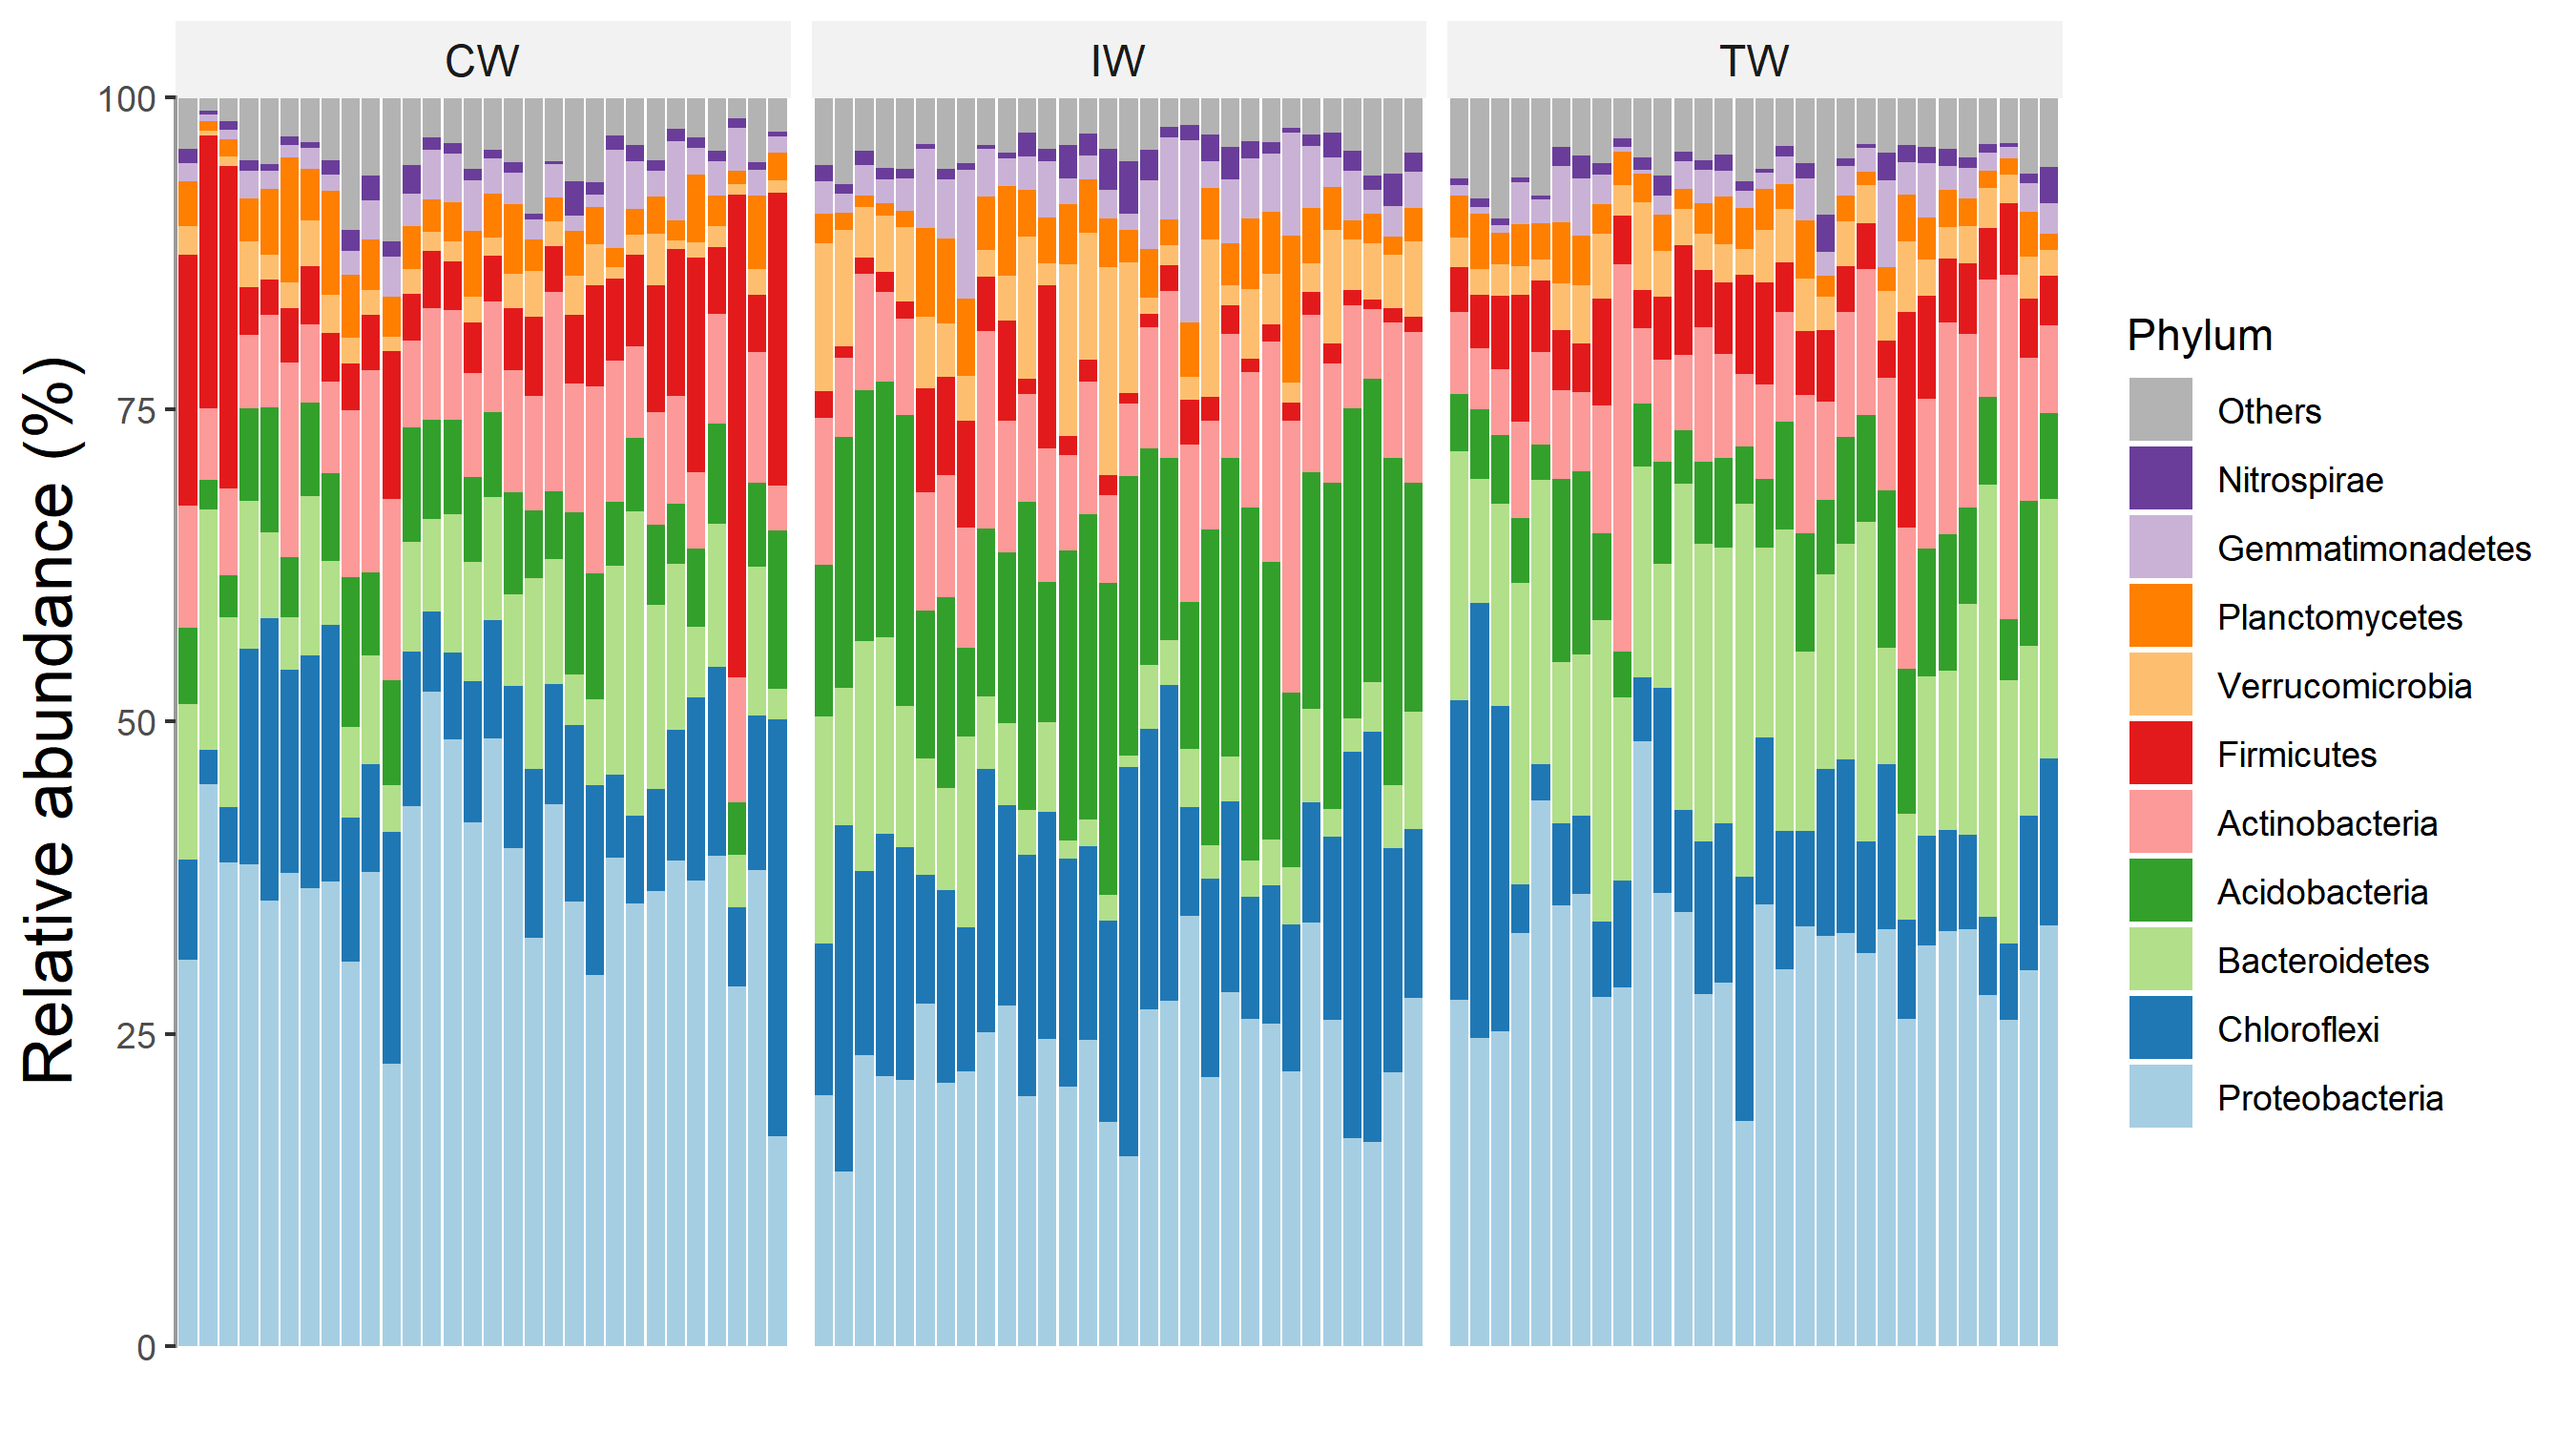
\includegraphics[width=750px]{Images/plot_bar} \end{center}

\begin{Shaded}
\begin{Highlighting}[]
\CommentTok{\# The groupmean parameter can be used to obtain the group{-}mean barplot.}
\NormalTok{t1 }\OtherTok{\textless{}{-}}\NormalTok{ trans\_abund}\SpecialCharTok{$}\FunctionTok{new}\NormalTok{(}\AttributeTok{dataset =}\NormalTok{ dataset, }\AttributeTok{taxrank =} \StringTok{"Phylum"}\NormalTok{, }\AttributeTok{ntaxa =} \DecValTok{10}\NormalTok{, }\AttributeTok{groupmean =} \StringTok{"Group"}\NormalTok{)}
\NormalTok{t1}\SpecialCharTok{$}\FunctionTok{plot\_bar}\NormalTok{(}\AttributeTok{others\_color =} \StringTok{"grey70"}\NormalTok{, }\AttributeTok{legend\_text\_italic =} \ConstantTok{FALSE}\NormalTok{)}
\end{Highlighting}
\end{Shaded}

\begin{center}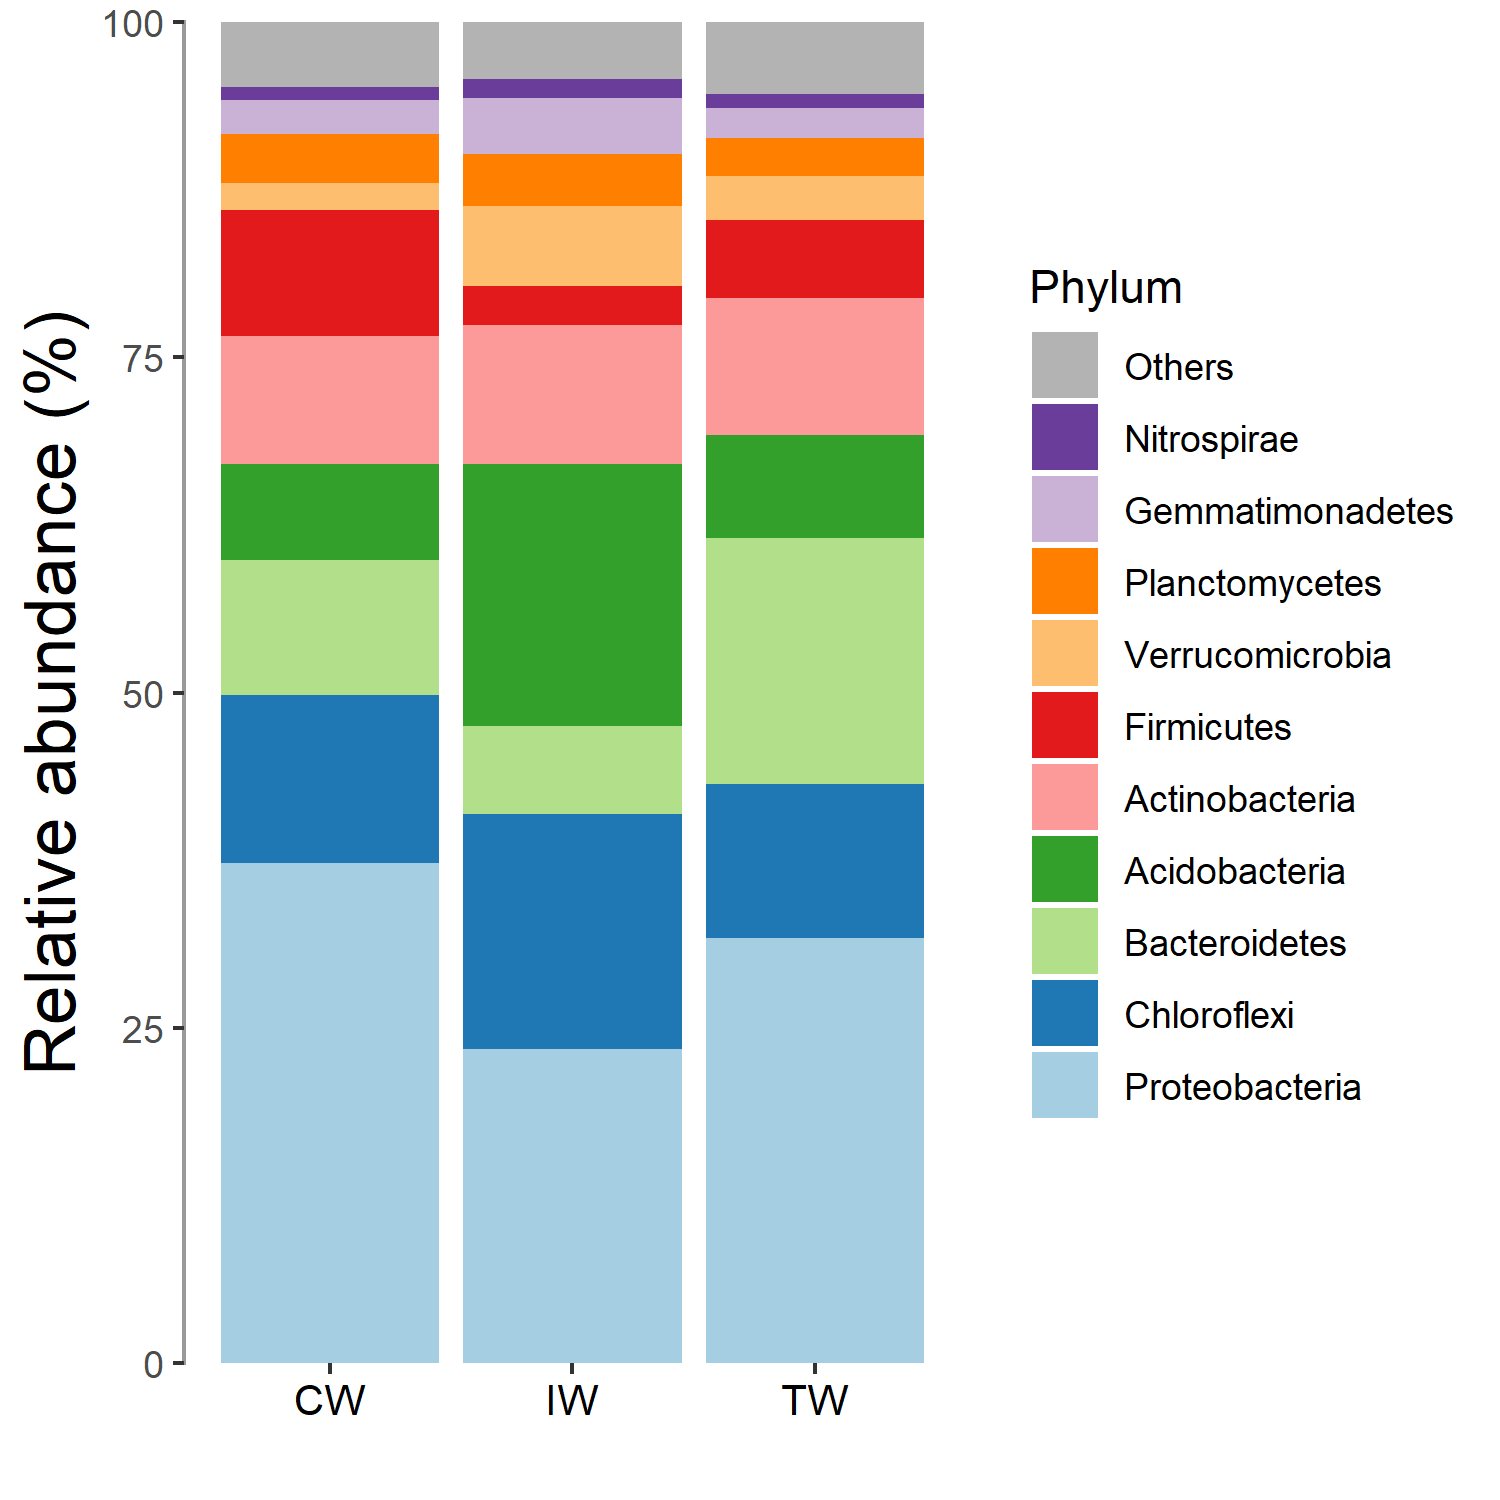
\includegraphics[width=400px]{Images/plot_bar_mean} \end{center}

Then alluvial plot is implemented in the plot\_bar function with the use\_alluvium parameter.

\begin{Shaded}
\begin{Highlighting}[]
\NormalTok{t1 }\OtherTok{\textless{}{-}}\NormalTok{ trans\_abund}\SpecialCharTok{$}\FunctionTok{new}\NormalTok{(}\AttributeTok{dataset =}\NormalTok{ dataset, }\AttributeTok{taxrank =} \StringTok{"Phylum"}\NormalTok{, }\AttributeTok{ntaxa =} \DecValTok{8}\NormalTok{)}
\CommentTok{\# use\_alluvium = TRUE make the alluvial plot, clustering = TRUE can be used to reorder the samples by clustering}
\NormalTok{t1}\SpecialCharTok{$}\FunctionTok{plot\_bar}\NormalTok{(}\AttributeTok{use\_alluvium =} \ConstantTok{TRUE}\NormalTok{, }\AttributeTok{clustering =} \ConstantTok{TRUE}\NormalTok{, }\AttributeTok{xtext\_type\_hor =} \ConstantTok{FALSE}\NormalTok{, }\AttributeTok{xtext\_size =} \DecValTok{6}\NormalTok{)}
\end{Highlighting}
\end{Shaded}

\begin{center}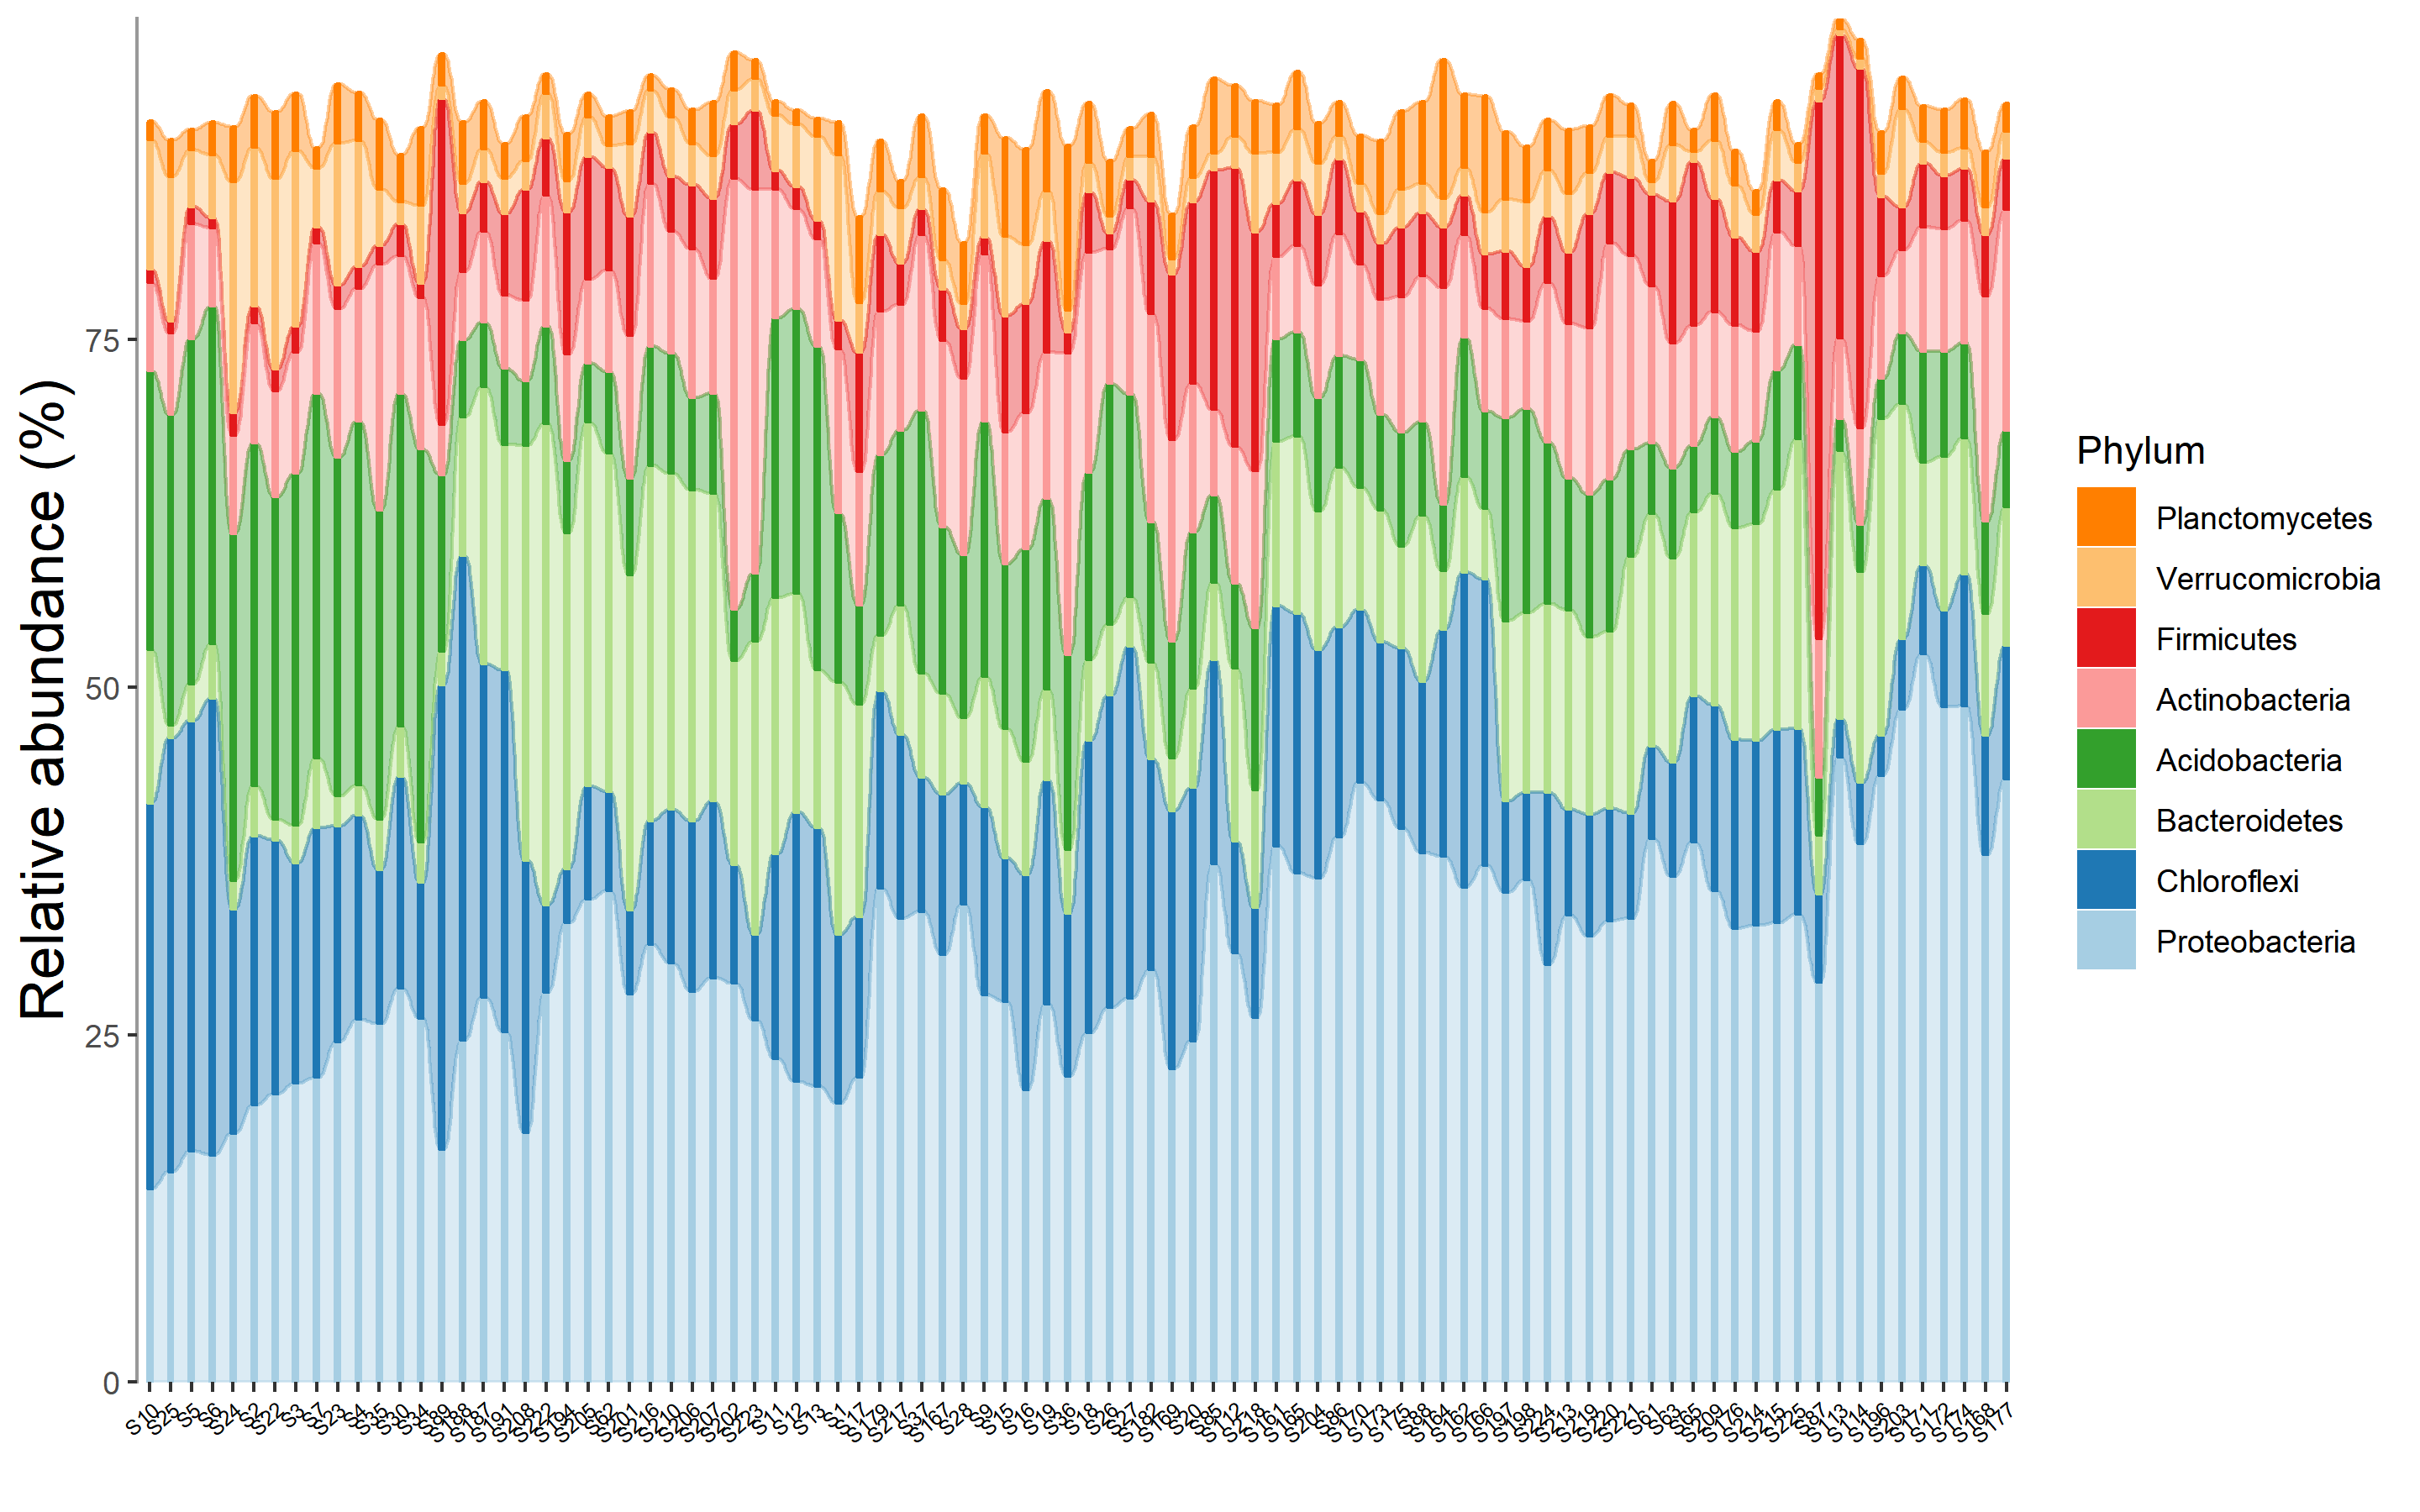
\includegraphics[width=40in]{Images/plot_bar_allu} \end{center}

The box plot is an excellent way to intuitionally show data distribution across groups.

\begin{Shaded}
\begin{Highlighting}[]
\CommentTok{\# show 15 taxa at Class level}
\NormalTok{t1 }\OtherTok{\textless{}{-}}\NormalTok{ trans\_abund}\SpecialCharTok{$}\FunctionTok{new}\NormalTok{(}\AttributeTok{dataset =}\NormalTok{ dataset, }\AttributeTok{taxrank =} \StringTok{"Class"}\NormalTok{, }\AttributeTok{ntaxa =} \DecValTok{15}\NormalTok{)}
\NormalTok{t1}\SpecialCharTok{$}\FunctionTok{plot\_box}\NormalTok{(}\AttributeTok{group =} \StringTok{"Group"}\NormalTok{)}
\end{Highlighting}
\end{Shaded}

\begin{center}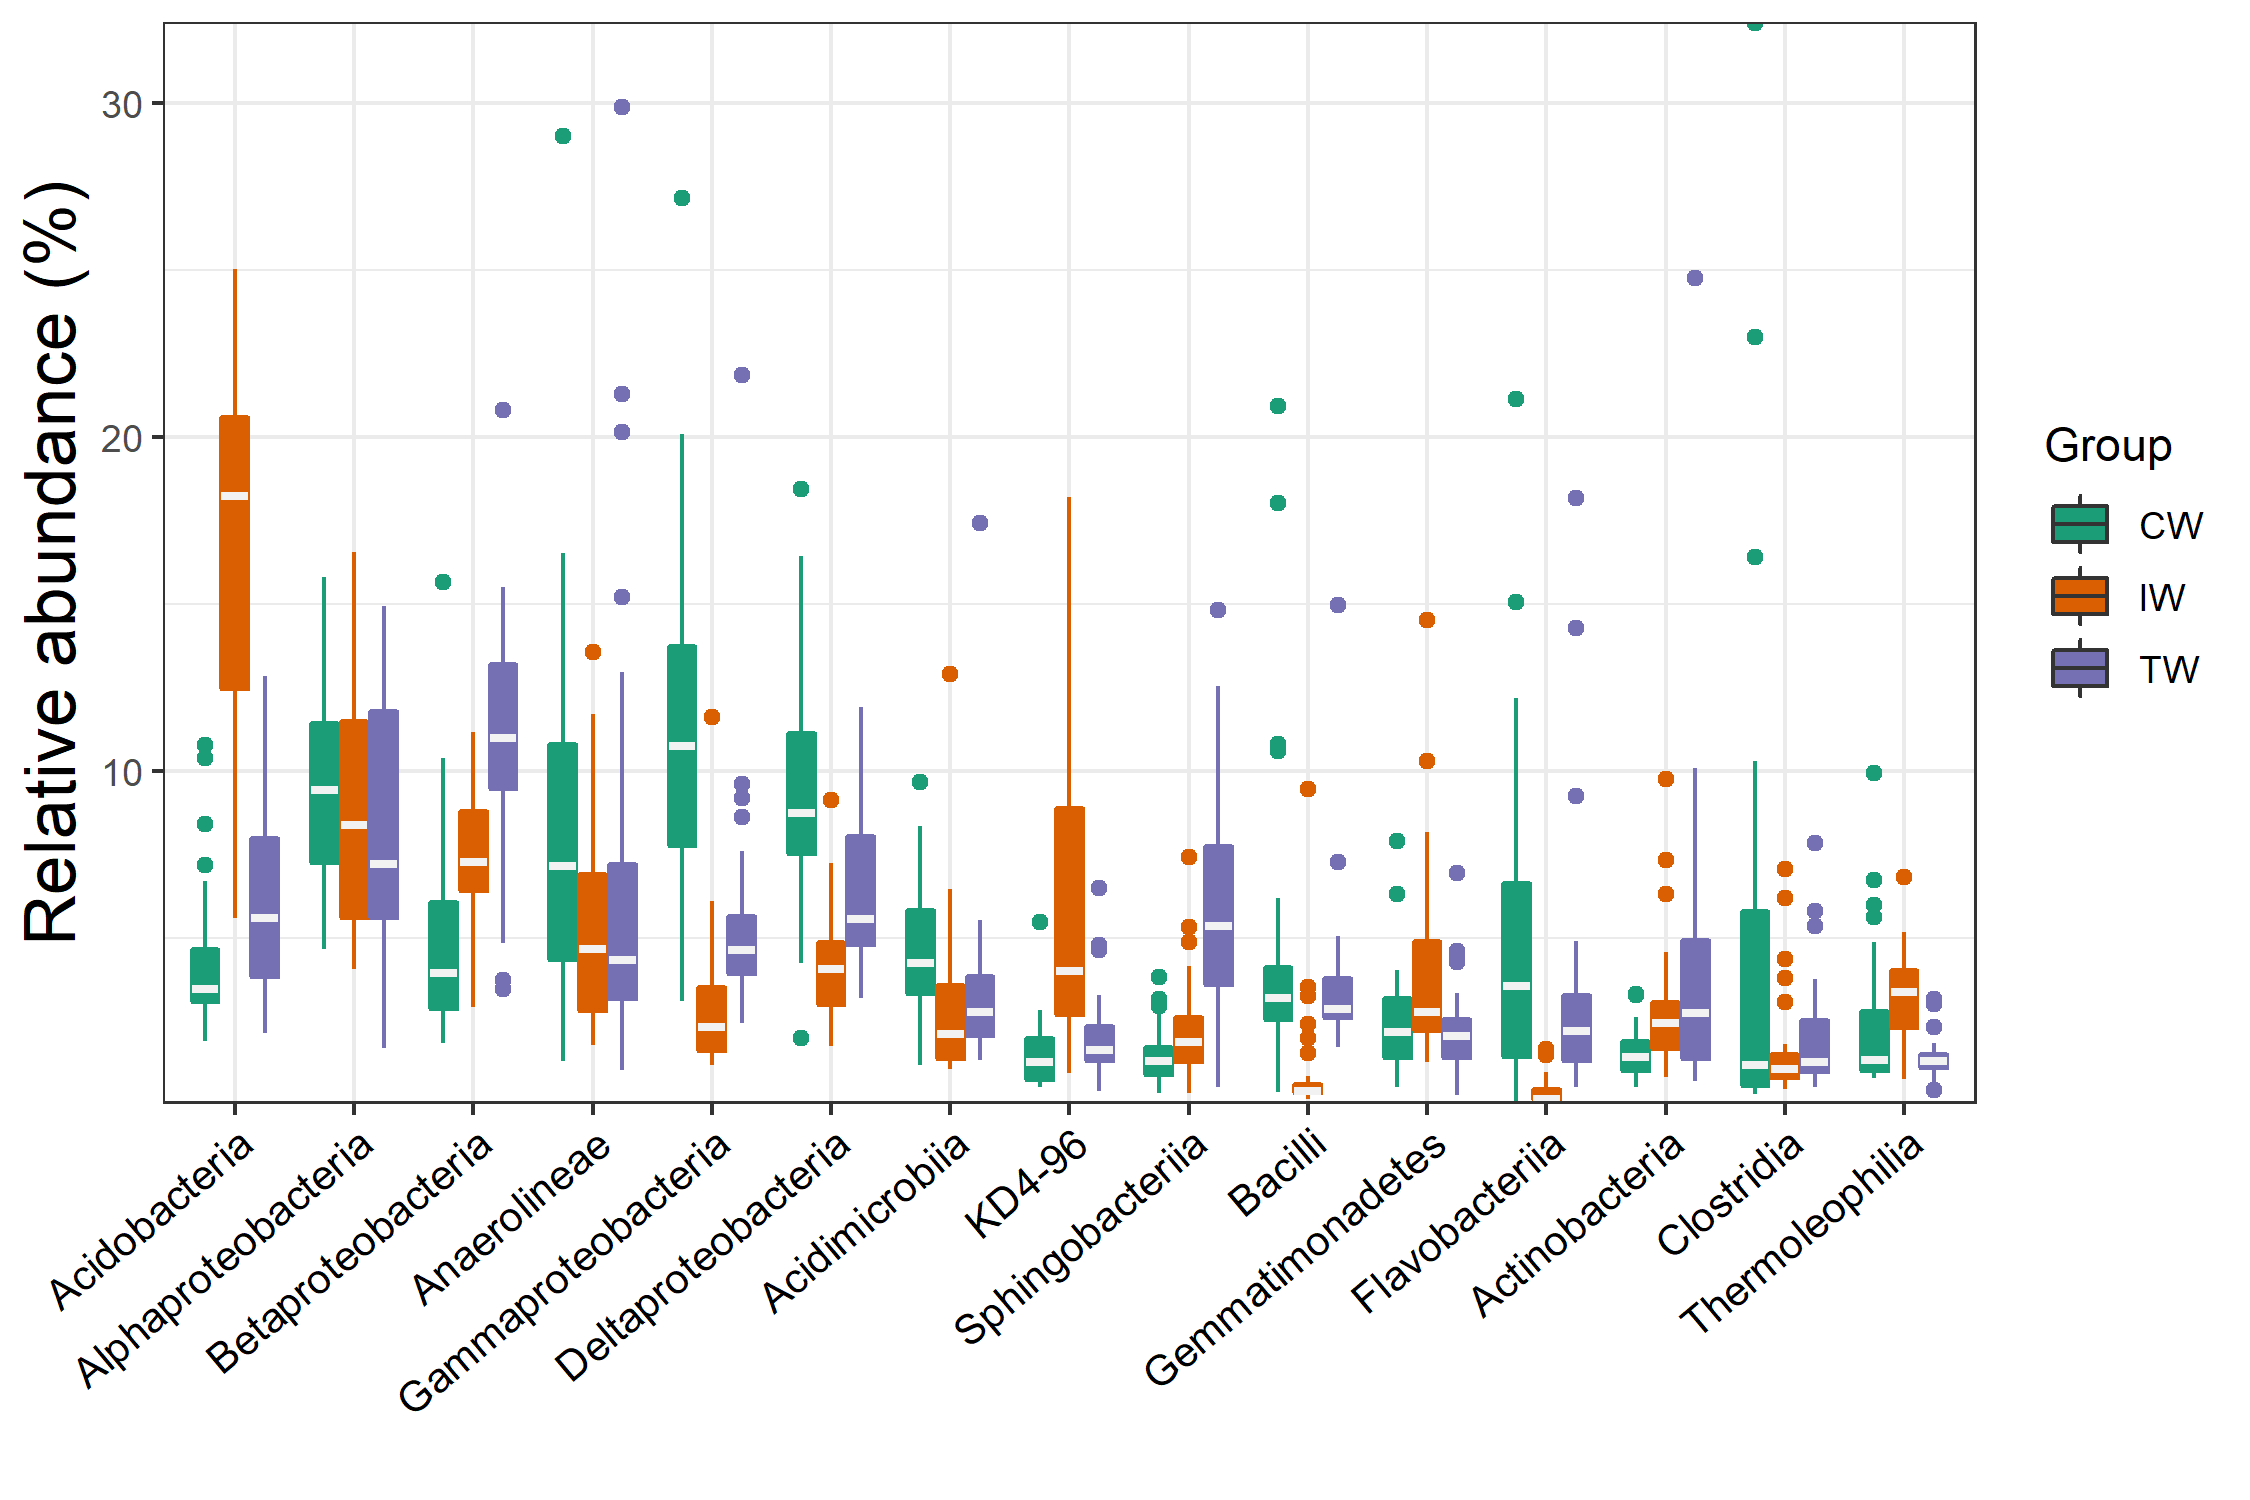
\includegraphics[width=700px]{Images/plot_box} \end{center}

Then we show the heatmap with the high abundant genera.

\begin{Shaded}
\begin{Highlighting}[]
\CommentTok{\# show 40 taxa at Genus level}
\NormalTok{t1 }\OtherTok{\textless{}{-}}\NormalTok{ trans\_abund}\SpecialCharTok{$}\FunctionTok{new}\NormalTok{(}\AttributeTok{dataset =}\NormalTok{ dataset, }\AttributeTok{taxrank =} \StringTok{"Genus"}\NormalTok{, }\AttributeTok{ntaxa =} \DecValTok{40}\NormalTok{)}
\NormalTok{t1}\SpecialCharTok{$}\FunctionTok{plot\_heatmap}\NormalTok{(}\AttributeTok{facet =} \StringTok{"Group"}\NormalTok{, }\AttributeTok{xtext\_keep =} \ConstantTok{FALSE}\NormalTok{, }\AttributeTok{withmargin =} \ConstantTok{FALSE}\NormalTok{)}
\end{Highlighting}
\end{Shaded}

\begin{center}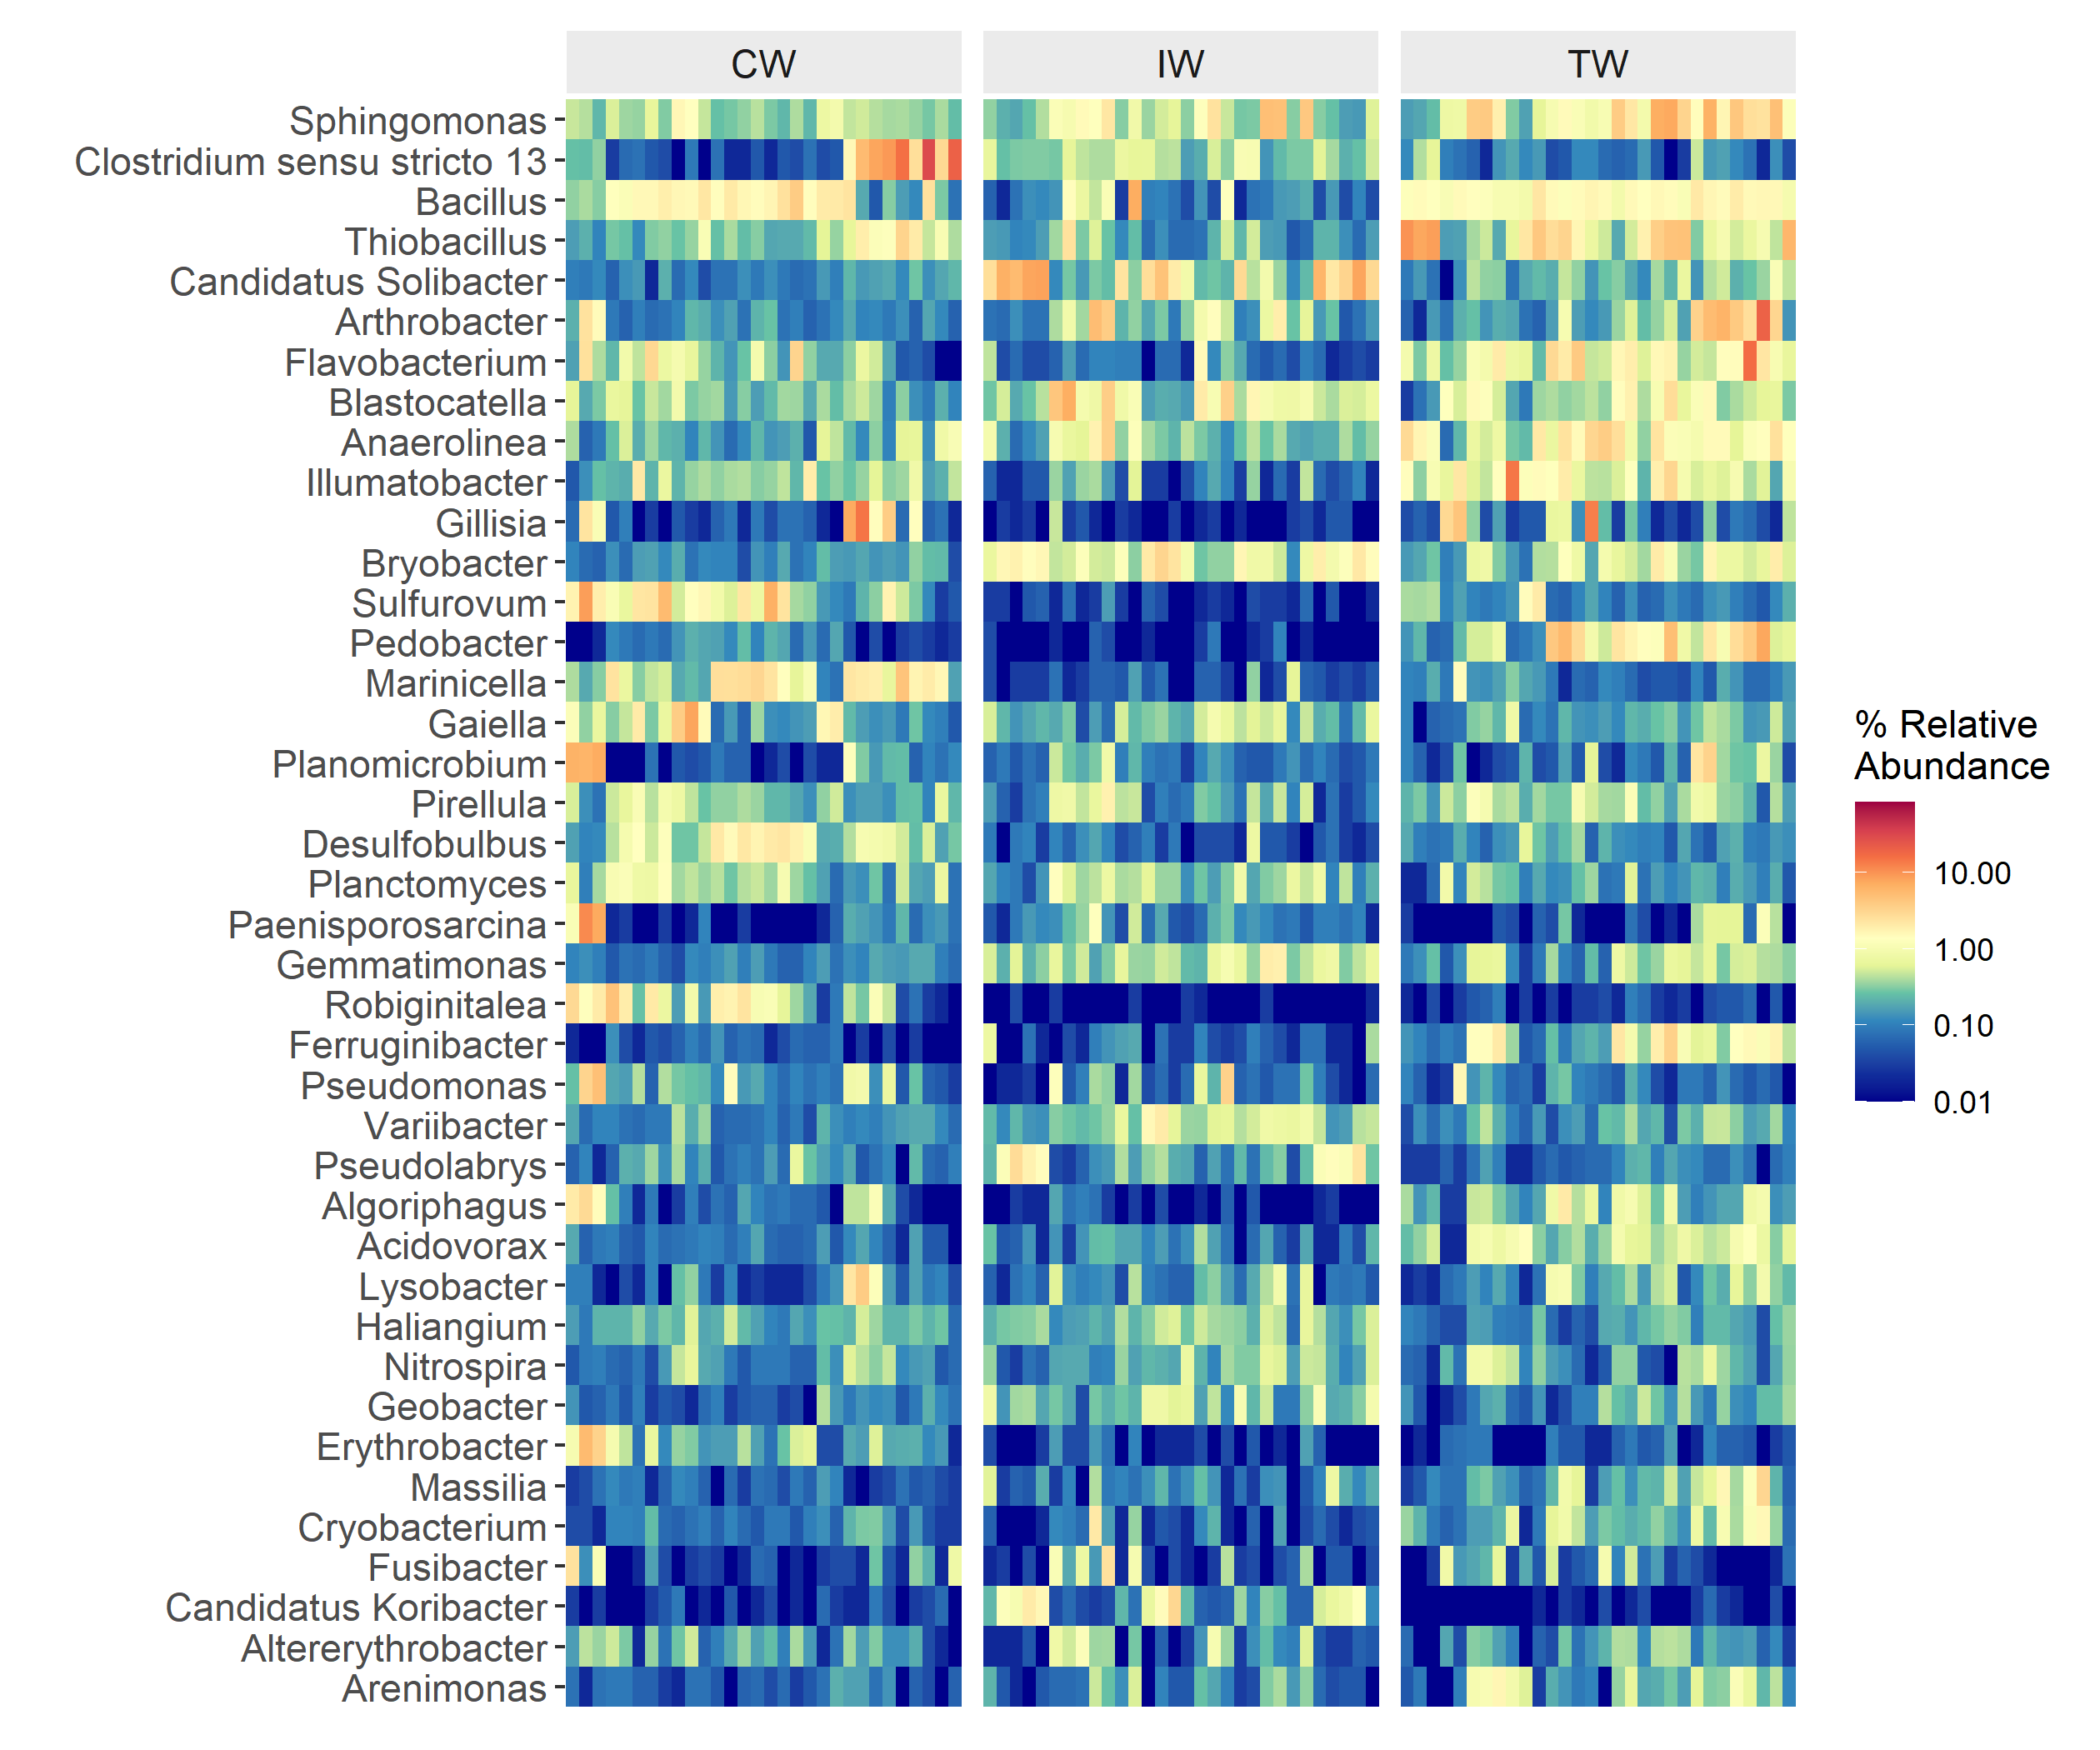
\includegraphics[width=750px]{Images/plot_heatmap} \end{center}

Then, we show the pie chart with the group mean values.

\begin{Shaded}
\begin{Highlighting}[]
\NormalTok{t1 }\OtherTok{\textless{}{-}}\NormalTok{ trans\_abund}\SpecialCharTok{$}\FunctionTok{new}\NormalTok{(}\AttributeTok{dataset =}\NormalTok{ dataset, }\AttributeTok{taxrank =} \StringTok{"Phylum"}\NormalTok{, }\AttributeTok{ntaxa =} \DecValTok{6}\NormalTok{, }\AttributeTok{groupmean =} \StringTok{"Group"}\NormalTok{)}
\CommentTok{\# all pie chart in one row}
\NormalTok{t1}\SpecialCharTok{$}\FunctionTok{plot\_pie}\NormalTok{(}\AttributeTok{facet\_nrow =} \DecValTok{1}\NormalTok{)}
\end{Highlighting}
\end{Shaded}

\begin{center}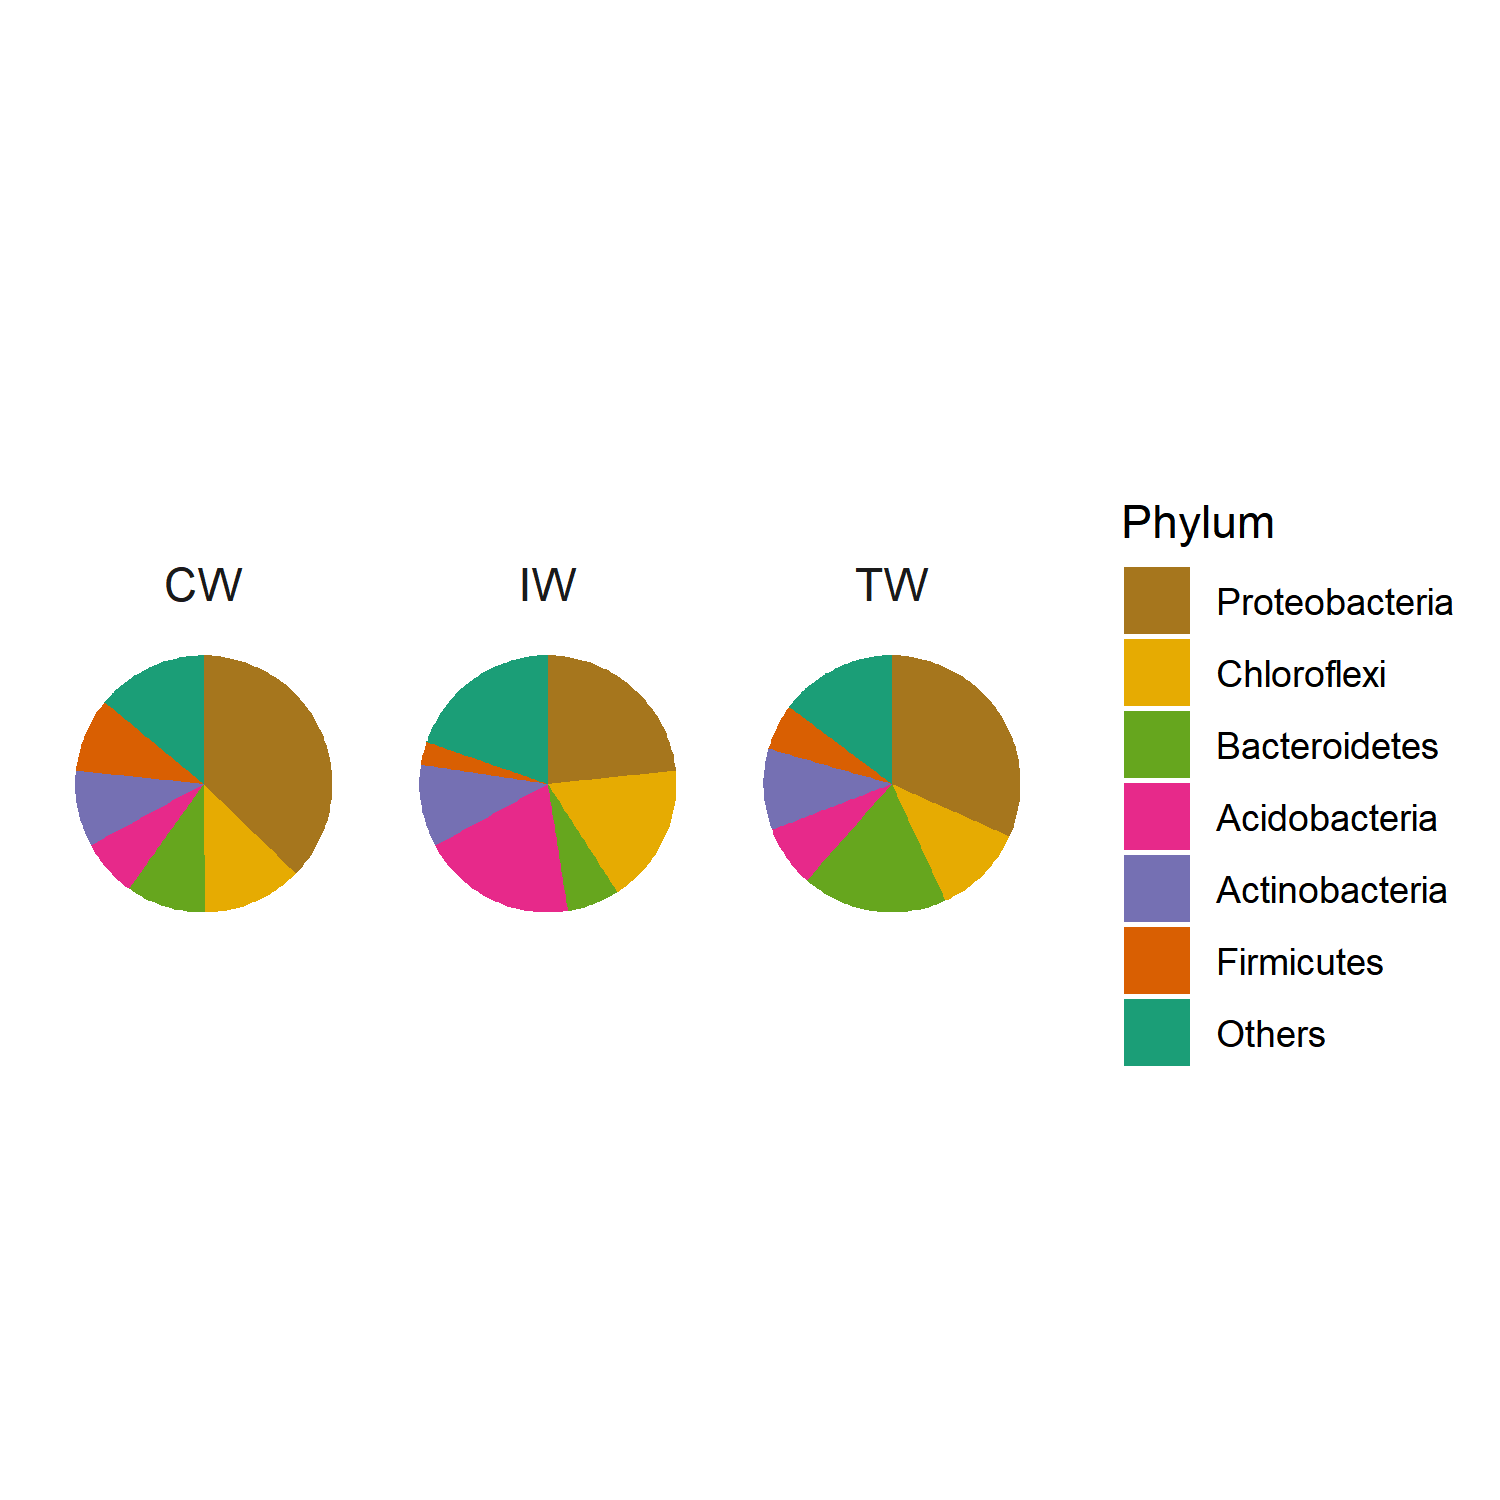
\includegraphics[width=600px]{Images/plot_pie} \end{center}

\hypertarget{trans_venn-class}{%
\section{trans\_venn class}\label{trans_venn-class}}

The trans\_venn class is used for venn analysis.
To analyze the unique and shared OTUs of groups,
we first merge samples according to the ``Group'' column of sample\_table.

\begin{Shaded}
\begin{Highlighting}[]
\CommentTok{\# merge samples as one community for each group}
\NormalTok{dataset1 }\OtherTok{\textless{}{-}}\NormalTok{ dataset}\SpecialCharTok{$}\FunctionTok{merge\_samples}\NormalTok{(}\AttributeTok{use\_group =} \StringTok{"Group"}\NormalTok{)}
\CommentTok{\# dataset1 is a new microtable object}
\CommentTok{\# create trans\_venn object}
\NormalTok{t1 }\OtherTok{\textless{}{-}}\NormalTok{ trans\_venn}\SpecialCharTok{$}\FunctionTok{new}\NormalTok{(dataset1, }\AttributeTok{ratio =} \StringTok{"seqratio"}\NormalTok{)}
\NormalTok{t1}\SpecialCharTok{$}\FunctionTok{plot\_venn}\NormalTok{()}
\CommentTok{\# The integer data is OTU number}
\CommentTok{\# The percentage data is the sequence number/total sequence number}
\end{Highlighting}
\end{Shaded}

\begin{center}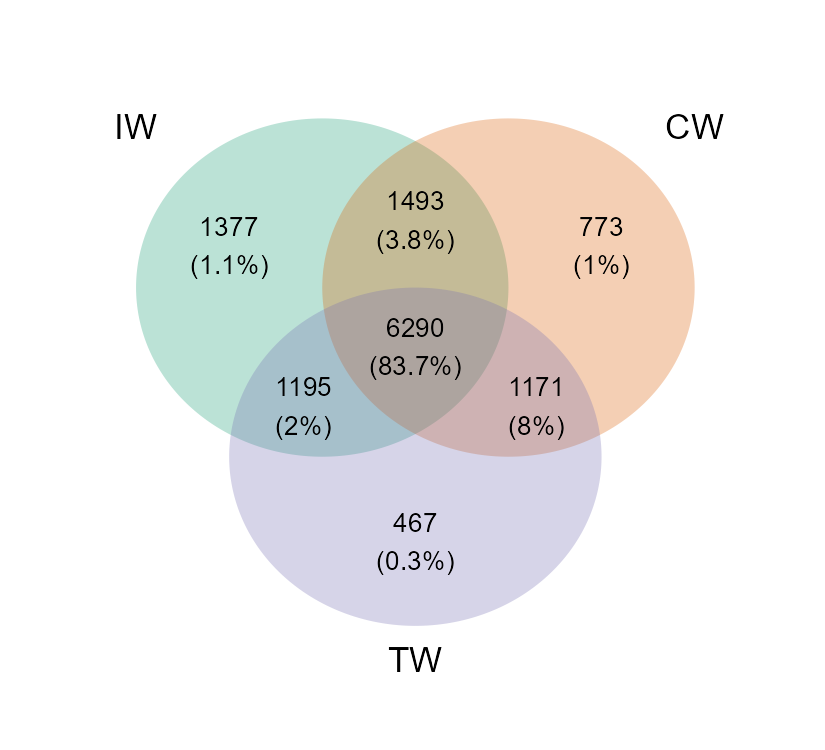
\includegraphics[width=500px]{Images/trans_venn_1} \end{center}

When the groups are too many to show with venn plot, we can use petal plot.

\begin{Shaded}
\begin{Highlighting}[]
\CommentTok{\# use "Type" column in sample\_table}
\NormalTok{dataset1 }\OtherTok{\textless{}{-}}\NormalTok{ dataset}\SpecialCharTok{$}\FunctionTok{merge\_samples}\NormalTok{(}\AttributeTok{use\_group =} \StringTok{"Type"}\NormalTok{)}
\NormalTok{t1 }\OtherTok{\textless{}{-}}\NormalTok{ trans\_venn}\SpecialCharTok{$}\FunctionTok{new}\NormalTok{(dataset1)}
\NormalTok{t1}\SpecialCharTok{$}\FunctionTok{plot\_venn}\NormalTok{(}\AttributeTok{petal\_plot =} \ConstantTok{TRUE}\NormalTok{)}
\end{Highlighting}
\end{Shaded}

\begin{center}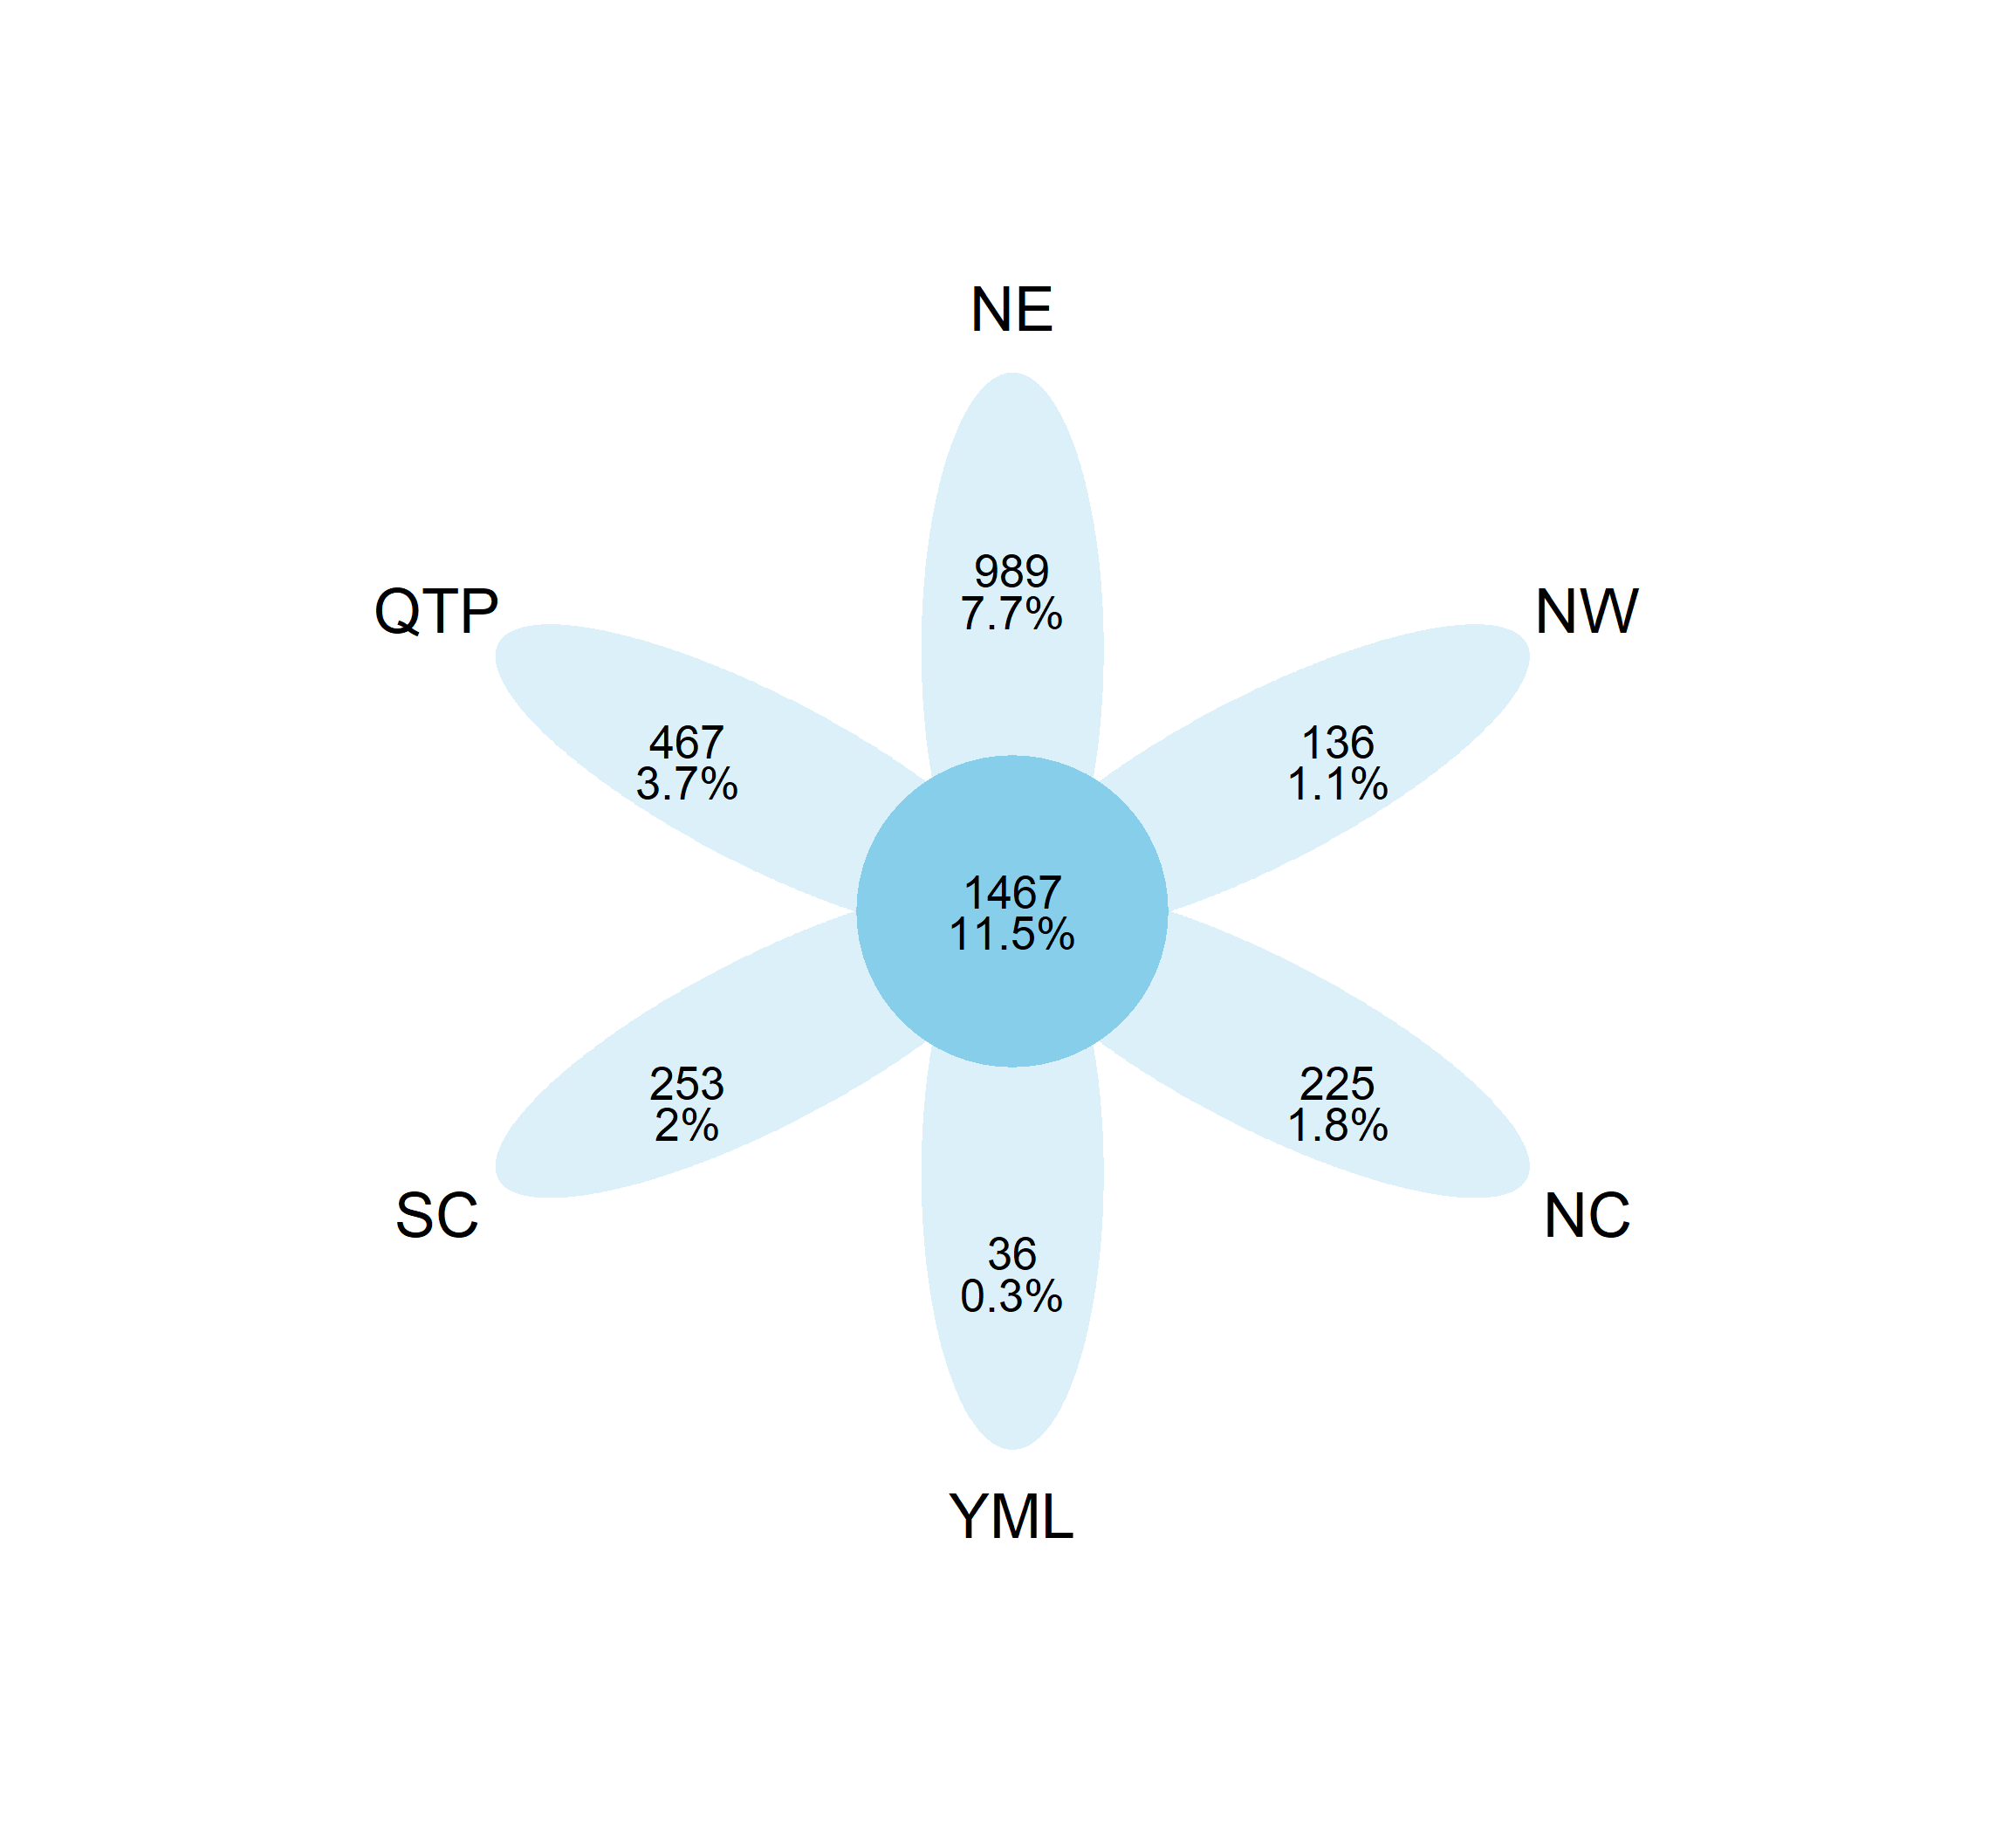
\includegraphics[width=500px]{Images/trans_venn_2} \end{center}

Sometimes, we are interested in the unique and shared species. In another words,
the composition of the unique or shared species may account for the different and similar parts of ecological characteristics across groups\citep{Mendes_Deciphering_2011}.
For this goal, we first transform the results of venn plot to the traditional species-sample table, that is, another object of microtable class.

\begin{Shaded}
\begin{Highlighting}[]
\NormalTok{dataset1 }\OtherTok{\textless{}{-}}\NormalTok{ dataset}\SpecialCharTok{$}\FunctionTok{merge\_samples}\NormalTok{(}\AttributeTok{use\_group =} \StringTok{"Group"}\NormalTok{)}
\NormalTok{t1 }\OtherTok{\textless{}{-}}\NormalTok{ trans\_venn}\SpecialCharTok{$}\FunctionTok{new}\NormalTok{(dataset1)}
\end{Highlighting}
\end{Shaded}

\begin{verbatim}
## The result is stored in object$venn_table and object$venn_count_abund ...
\end{verbatim}

\begin{Shaded}
\begin{Highlighting}[]
\CommentTok{\# transform venn results to the sample{-}species table, here do not consider abundance, only use presence/absence information.}
\NormalTok{t2 }\OtherTok{\textless{}{-}}\NormalTok{ t1}\SpecialCharTok{$}\FunctionTok{trans\_venn\_com}\NormalTok{(}\AttributeTok{use\_OTUs\_frequency =} \ConstantTok{TRUE}\NormalTok{)}
\CommentTok{\# t2 is a new microtable class, each part is considered as a sample}
\FunctionTok{class}\NormalTok{(t2)}
\end{Highlighting}
\end{Shaded}

\begin{verbatim}
## [1] "microtable" "R6"
\end{verbatim}

We use bar plot to show the composition at the Genus level.

\begin{Shaded}
\begin{Highlighting}[]
\CommentTok{\# calculate taxa abundance, that is, the frequency}
\NormalTok{t2}\SpecialCharTok{$}\FunctionTok{cal\_abund}\NormalTok{()}
\CommentTok{\# transform and plot}
\NormalTok{t3 }\OtherTok{\textless{}{-}}\NormalTok{ trans\_abund}\SpecialCharTok{$}\FunctionTok{new}\NormalTok{(}\AttributeTok{dataset =}\NormalTok{ t2, }\AttributeTok{taxrank =} \StringTok{"Genus"}\NormalTok{, }\AttributeTok{ntaxa =} \DecValTok{10}\NormalTok{)}
\NormalTok{t3}\SpecialCharTok{$}\FunctionTok{plot\_bar}\NormalTok{(}\AttributeTok{bar\_type =} \StringTok{"part"}\NormalTok{, }\AttributeTok{legend\_text\_italic =}\NormalTok{ T, }\AttributeTok{ylab\_title =} \StringTok{"Frequency (\%)"}\NormalTok{, }\AttributeTok{xtext\_type\_hor =} \ConstantTok{FALSE}\NormalTok{)}
\end{Highlighting}
\end{Shaded}

\begin{center}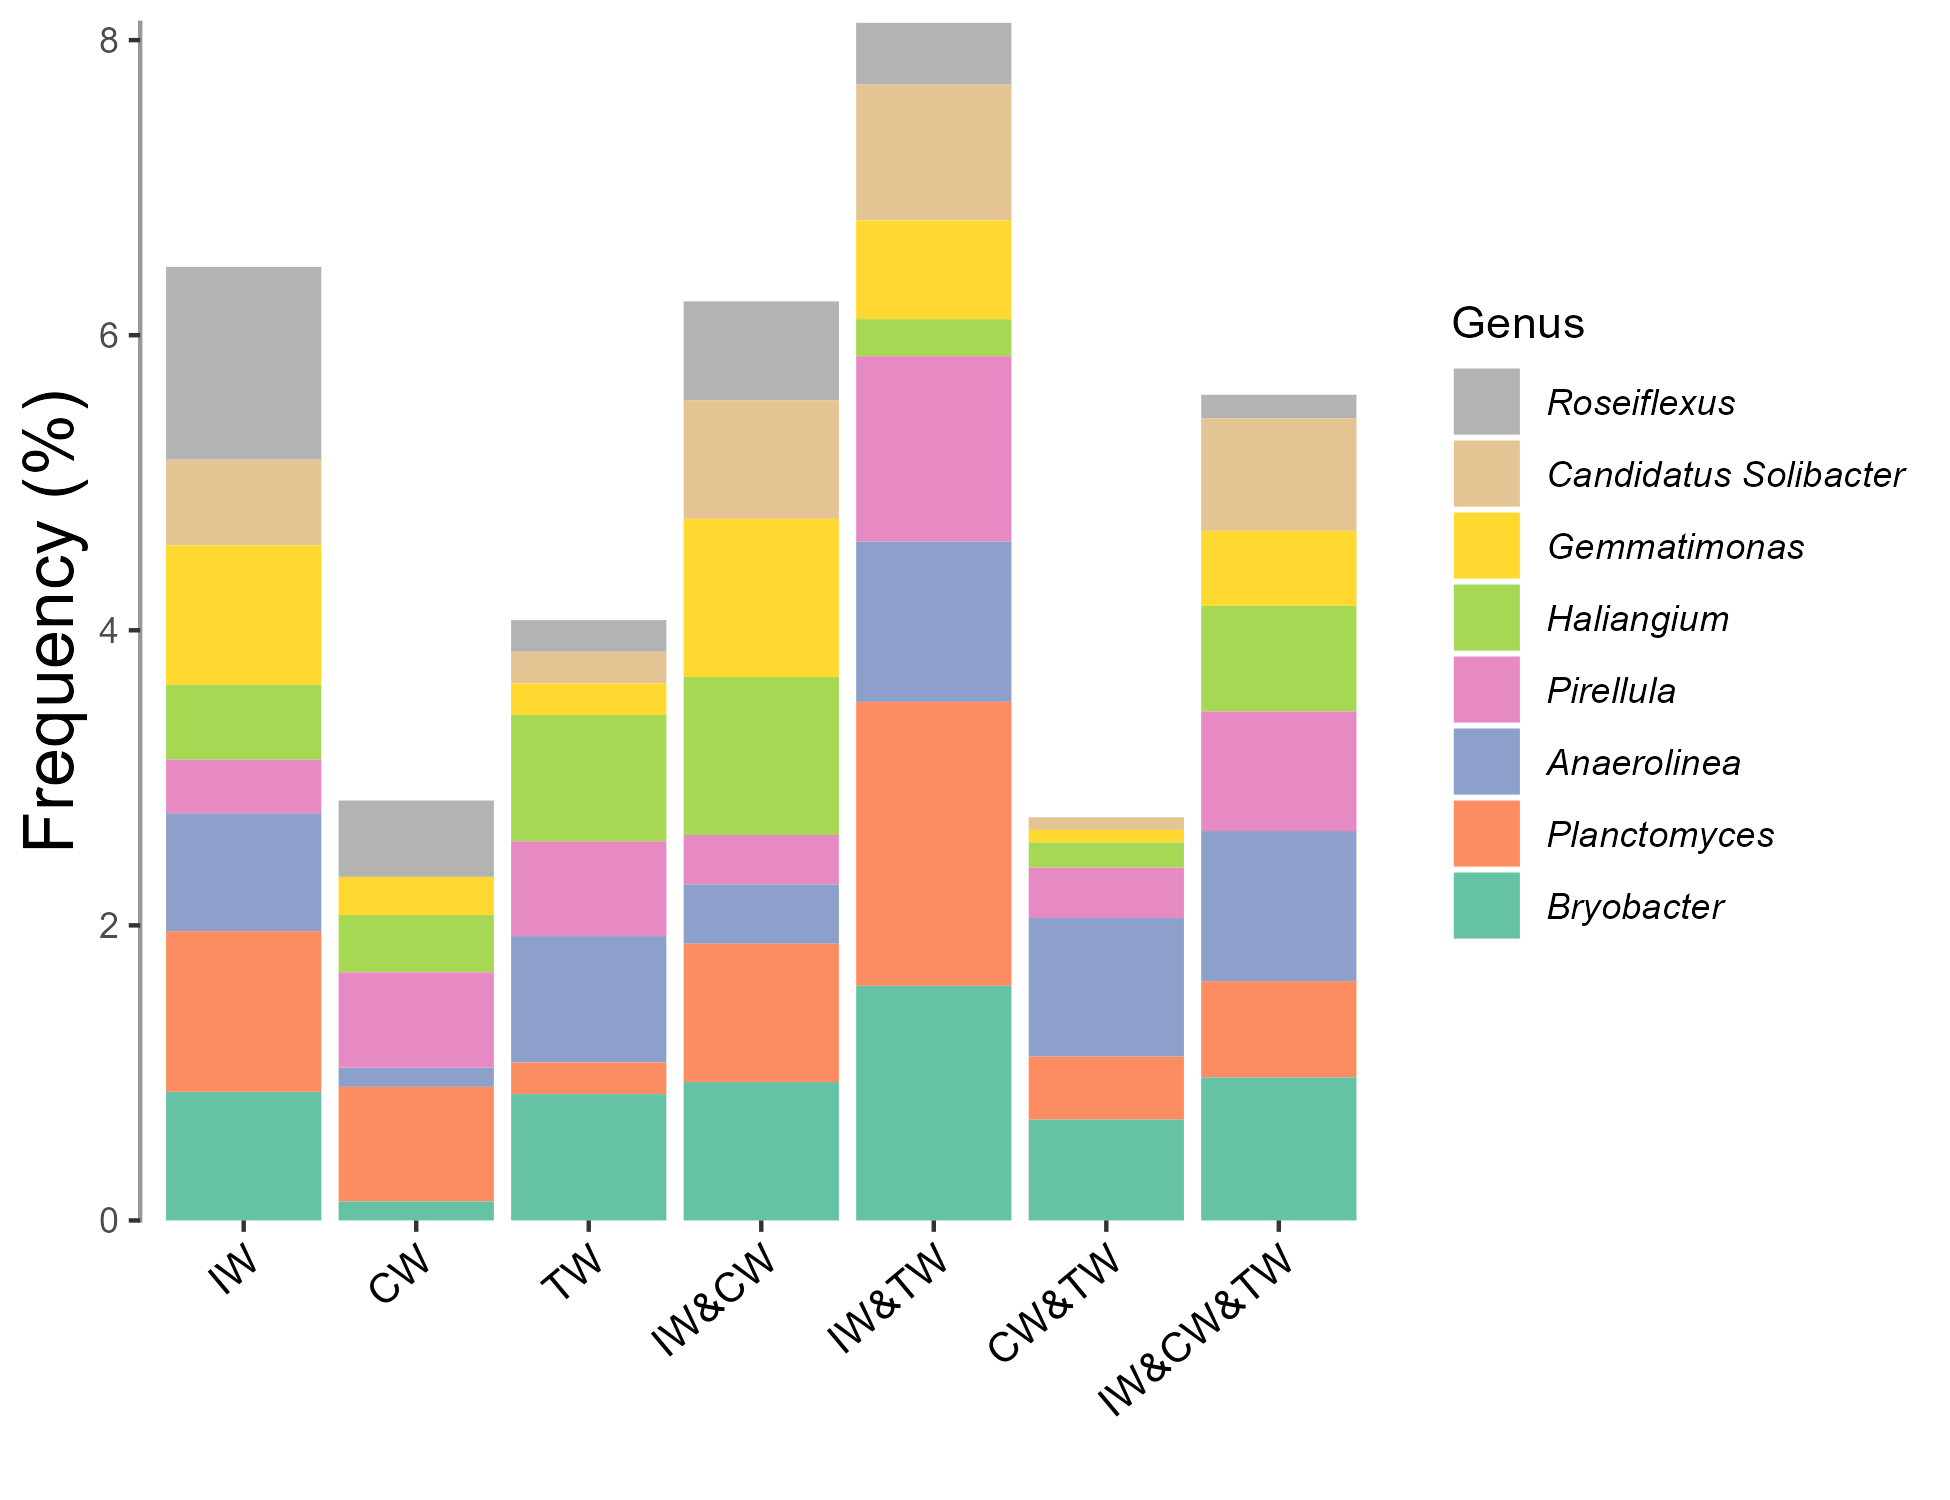
\includegraphics[width=650px]{Images/trans_venn_bar} \end{center}

We also try to use pie chart to show the compositions at the Phylum level.

\begin{Shaded}
\begin{Highlighting}[]
\NormalTok{t3 }\OtherTok{\textless{}{-}}\NormalTok{ trans\_abund}\SpecialCharTok{$}\FunctionTok{new}\NormalTok{(}\AttributeTok{dataset =}\NormalTok{ t2, }\AttributeTok{taxrank =} \StringTok{"Phylum"}\NormalTok{, }\AttributeTok{ntaxa =} \DecValTok{8}\NormalTok{)}
\NormalTok{t3}\SpecialCharTok{$}\FunctionTok{plot\_pie}\NormalTok{(}\AttributeTok{facet\_nrow =} \DecValTok{3}\NormalTok{, }\AttributeTok{use\_colors =} \FunctionTok{rev}\NormalTok{(}\FunctionTok{c}\NormalTok{(RColorBrewer}\SpecialCharTok{::}\FunctionTok{brewer.pal}\NormalTok{(}\DecValTok{8}\NormalTok{, }\StringTok{"Dark2"}\NormalTok{), }\StringTok{"grey50"}\NormalTok{)))}
\end{Highlighting}
\end{Shaded}

\begin{center}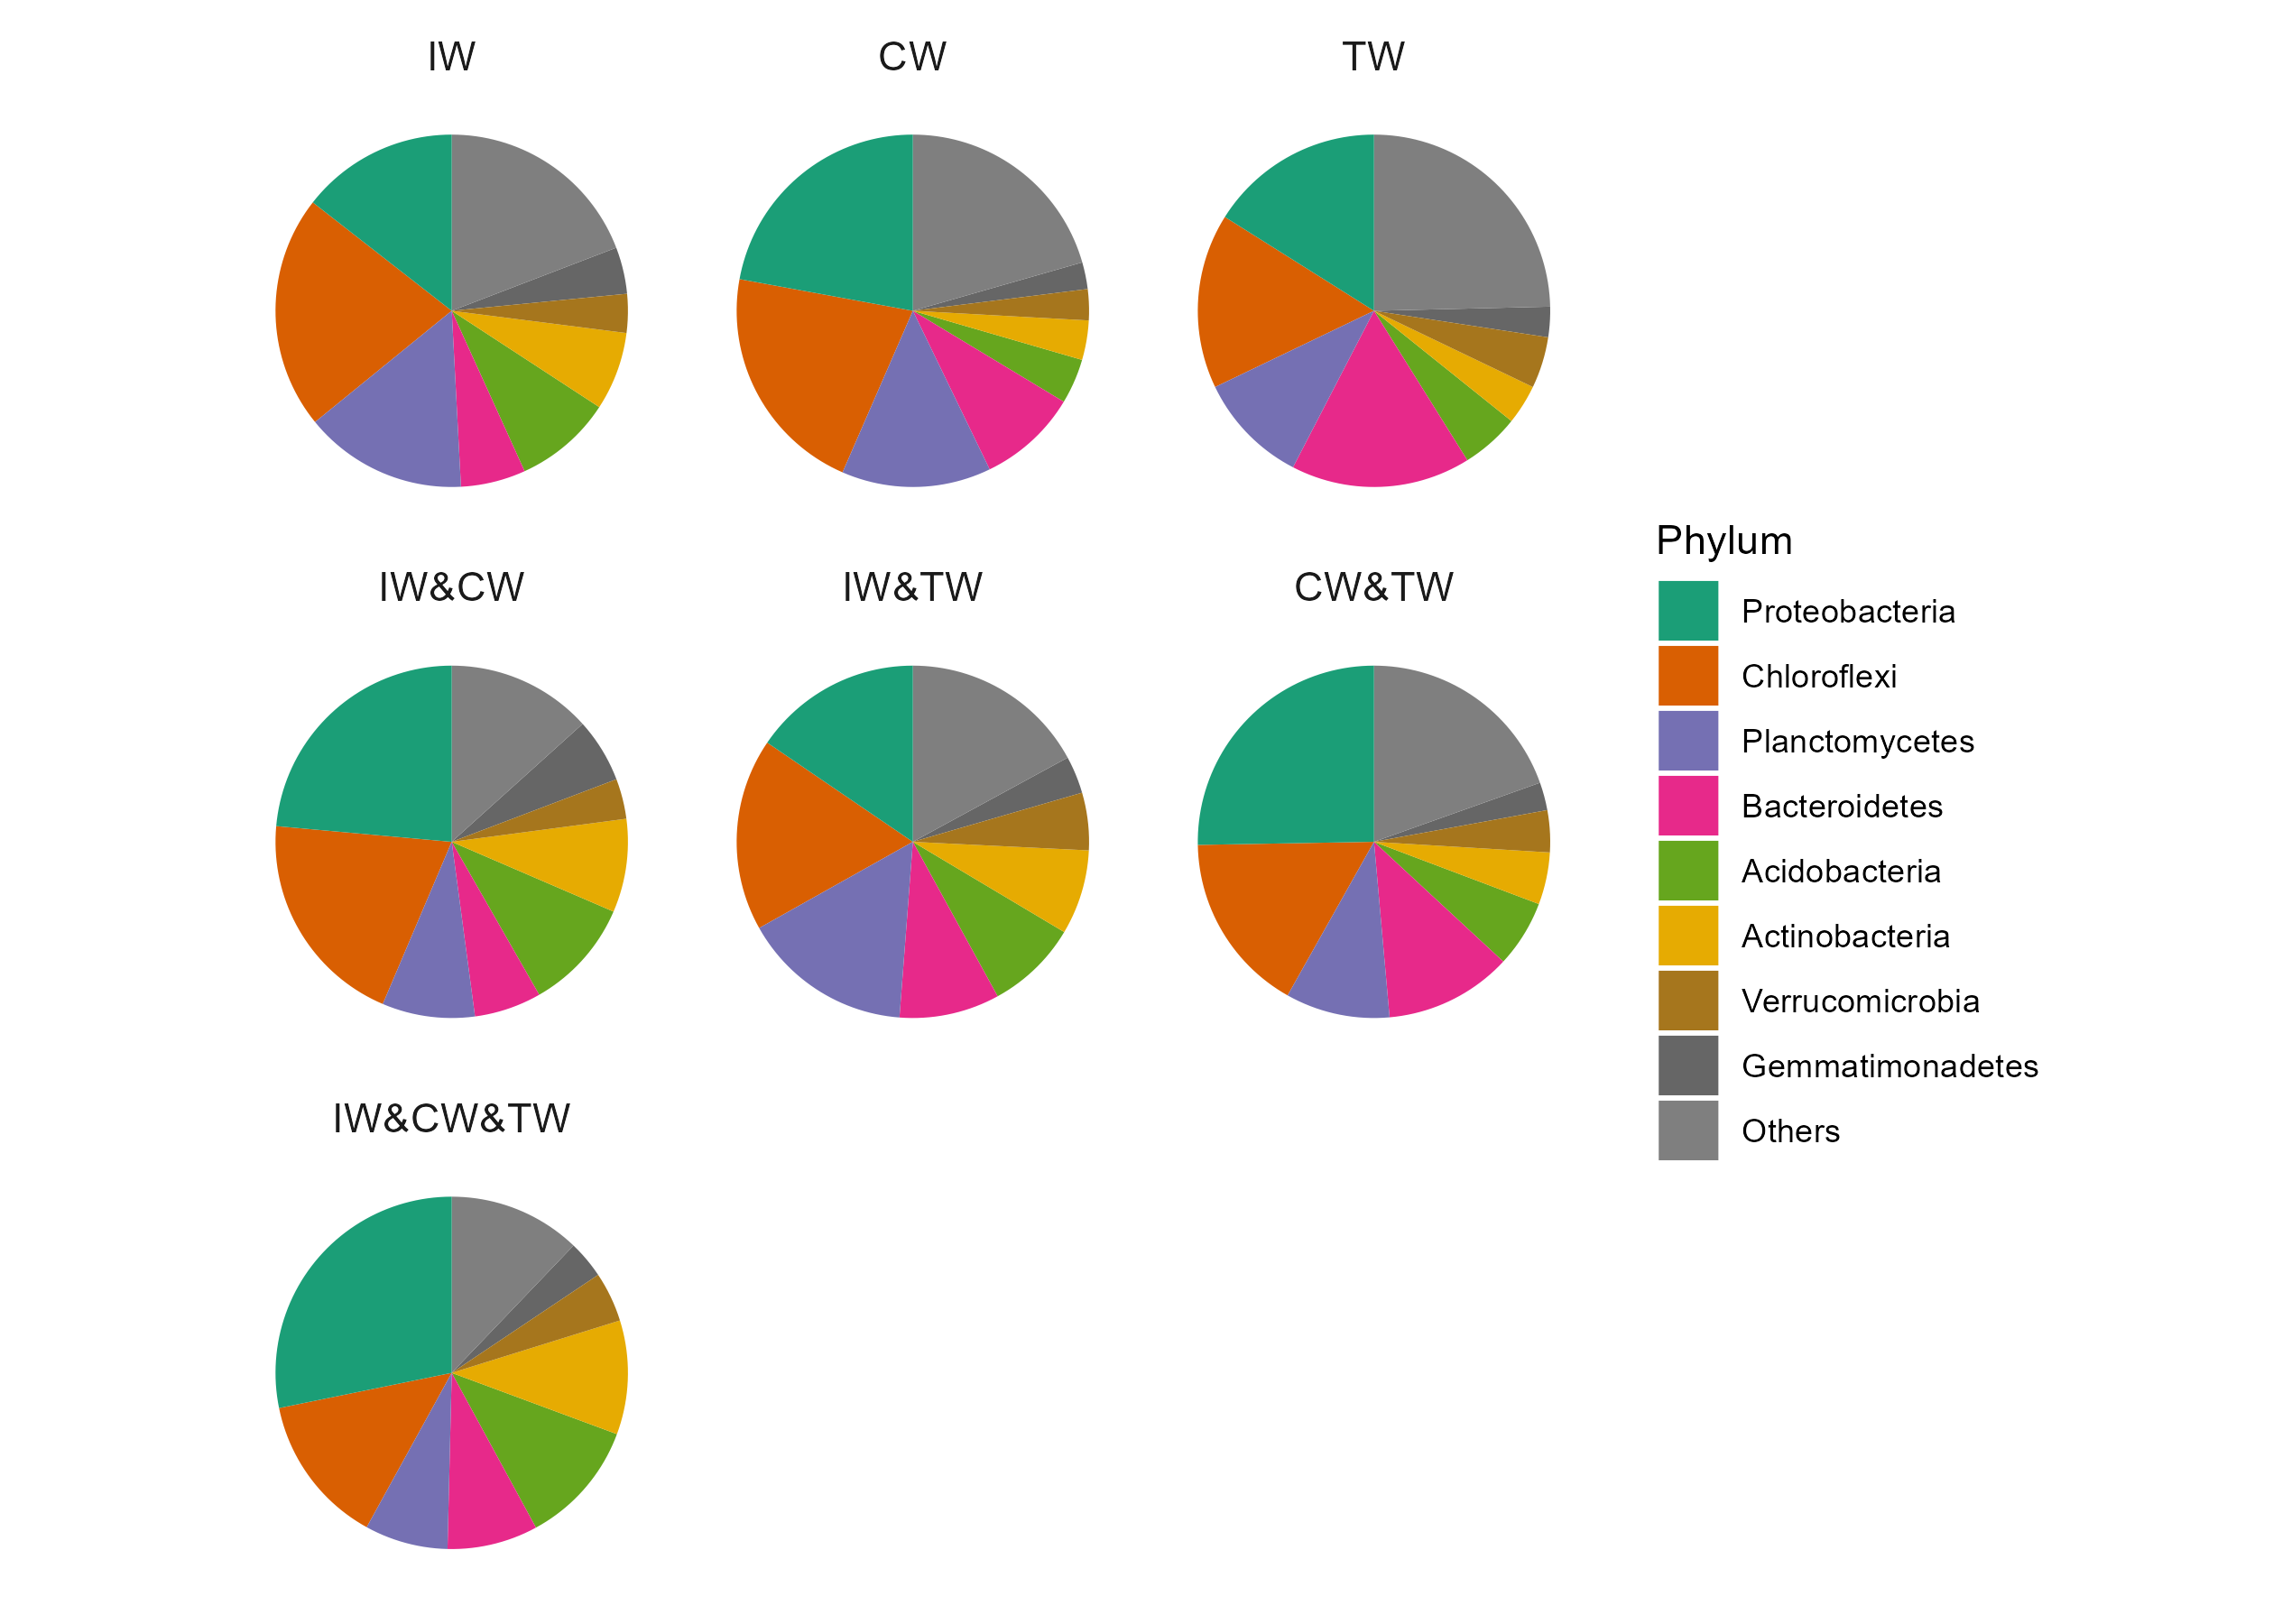
\includegraphics[width=800px]{Images/trans_venn_pie} \end{center}

\hypertarget{trans_alpha-class}{%
\section{trans\_alpha class}\label{trans_alpha-class}}

 Alpha diversity can be transformed and plotted using trans\_alpha class.
Creating the object of trans\_alpha class can invoke the alpha\_diversity data from the microtable object.
The trans\_alpha object have two data frame: alpha\_data and alpha\_stat.

\begin{Shaded}
\begin{Highlighting}[]
\NormalTok{t1 }\OtherTok{\textless{}{-}}\NormalTok{ trans\_alpha}\SpecialCharTok{$}\FunctionTok{new}\NormalTok{(}\AttributeTok{dataset =}\NormalTok{ dataset, }\AttributeTok{group =} \StringTok{"Group"}\NormalTok{)}
\CommentTok{\# return t1$alpha\_stat}
\NormalTok{t1}\SpecialCharTok{$}\NormalTok{alpha\_stat[}\DecValTok{1}\SpecialCharTok{:}\DecValTok{5}\NormalTok{, ]}
\end{Highlighting}
\end{Shaded}

\begin{verbatim}
## The group statistics are stored in object$alpha_stat ...
\end{verbatim}

\begin{verbatim}
## The transformed diversity data is stored in object$alpha_data ...
\end{verbatim}

\begin{longtable}[]{@{}
  >{\centering\arraybackslash}p{(\columnwidth - 10\tabcolsep) * \real{0.11}}
  >{\centering\arraybackslash}p{(\columnwidth - 10\tabcolsep) * \real{0.15}}
  >{\centering\arraybackslash}p{(\columnwidth - 10\tabcolsep) * \real{0.07}}
  >{\centering\arraybackslash}p{(\columnwidth - 10\tabcolsep) * \real{0.12}}
  >{\centering\arraybackslash}p{(\columnwidth - 10\tabcolsep) * \real{0.14}}
  >{\centering\arraybackslash}p{(\columnwidth - 10\tabcolsep) * \real{0.15}}@{}}
\toprule
Group & Measure & N & Mean & SD & SE \\
\midrule
\endhead
CW & Observed & 30 & 1843 & 220.6 & 40.27 \\
CW & Chao1 & 30 & 2553 & 338.1 & 61.73 \\
CW & ACE & 30 & 2716 & 367 & 67.01 \\
CW & Shannon & 30 & 6.308 & 0.5355 & 0.09777 \\
CW & Simpson & 30 & 0.9897 & 0.01305 & 0.002382 \\
\bottomrule
\end{longtable}

Then, we test the differences among groups using the KW rank sum test and anova with multiple comparisons.

\begin{Shaded}
\begin{Highlighting}[]
\NormalTok{t1}\SpecialCharTok{$}\FunctionTok{cal\_diff}\NormalTok{(}\AttributeTok{method =} \StringTok{"KW"}\NormalTok{)}
\CommentTok{\# return t1$res\_alpha\_diff}
\NormalTok{t1}\SpecialCharTok{$}\NormalTok{res\_alpha\_diff[}\DecValTok{1}\SpecialCharTok{:}\DecValTok{5}\NormalTok{, ]}
\end{Highlighting}
\end{Shaded}

\begin{verbatim}
## The result is stored in object$res_alpha_diff ...
\end{verbatim}

\begin{longtable}[]{@{}
  >{\centering\arraybackslash}p{(\columnwidth - 8\tabcolsep) * \real{0.24}}
  >{\centering\arraybackslash}p{(\columnwidth - 8\tabcolsep) * \real{0.15}}
  >{\centering\arraybackslash}p{(\columnwidth - 8\tabcolsep) * \real{0.19}}
  >{\centering\arraybackslash}p{(\columnwidth - 8\tabcolsep) * \real{0.15}}
  >{\centering\arraybackslash}p{(\columnwidth - 8\tabcolsep) * \real{0.21}}@{}}
\toprule
Groups & Measure & Test method & p.value & Significance \\
\midrule
\endhead
IW vs CW & Observed & KW & 0.0371 & * \\
IW vs TW & Observed & KW & 0.4553 & \\
CW vs TW & Observed & KW & 0.3912 & \\
IW vs CW vs TW & Observed & KW & 0.155 & \\
IW vs CW & Chao1 & KW & 0.002689 & ** \\
\bottomrule
\end{longtable}

\begin{Shaded}
\begin{Highlighting}[]
\NormalTok{t1}\SpecialCharTok{$}\FunctionTok{cal\_diff}\NormalTok{(}\AttributeTok{method =} \StringTok{"anova"}\NormalTok{)}
\CommentTok{\# return t1$res\_alpha\_diff}
\NormalTok{t1}\SpecialCharTok{$}\NormalTok{res\_alpha\_diff}
\end{Highlighting}
\end{Shaded}

\begin{verbatim}
## Registered S3 methods overwritten by 'klaR':
##   method      from 
##   predict.rda vegan
##   print.rda   vegan
##   plot.rda    vegan
\end{verbatim}

\begin{verbatim}
## The result is stored in object$res_alpha_diff ...
\end{verbatim}

\begin{longtable}[]{@{}
  >{\centering\arraybackslash}p{(\columnwidth - 16\tabcolsep) * \real{0.10}}
  >{\centering\arraybackslash}p{(\columnwidth - 16\tabcolsep) * \real{0.13}}
  >{\centering\arraybackslash}p{(\columnwidth - 16\tabcolsep) * \real{0.09}}
  >{\centering\arraybackslash}p{(\columnwidth - 16\tabcolsep) * \real{0.07}}
  >{\centering\arraybackslash}p{(\columnwidth - 16\tabcolsep) * \real{0.11}}
  >{\centering\arraybackslash}p{(\columnwidth - 16\tabcolsep) * \real{0.11}}
  >{\centering\arraybackslash}p{(\columnwidth - 16\tabcolsep) * \real{0.15}}
  >{\centering\arraybackslash}p{(\columnwidth - 16\tabcolsep) * \real{0.10}}
  >{\centering\arraybackslash}p{(\columnwidth - 16\tabcolsep) * \real{0.13}}@{}}
\toprule
~ & Observed & Chao1 & ACE & Shannon & Simpson & InvSimpson & Fisher & Coverage \\
\midrule
\endhead
\textbf{IW} & a & a & a & a & a & a & a & b \\
\textbf{TW} & a & ab & b & a & a & a & a & a \\
\textbf{CW} & a & b & b & a & a & a & a & a \\
\bottomrule
\end{longtable}

Now, let us plot the mean and se of alpha diversity for each group, and add the duncan.test (agricolae package) result.

\begin{Shaded}
\begin{Highlighting}[]
\NormalTok{t1}\SpecialCharTok{$}\FunctionTok{plot\_alpha}\NormalTok{(}\AttributeTok{add\_letter =}\NormalTok{ T, }\AttributeTok{measure =} \StringTok{"Chao1"}\NormalTok{, }\AttributeTok{use\_boxplot =} \ConstantTok{FALSE}\NormalTok{)}
\end{Highlighting}
\end{Shaded}

\begin{center}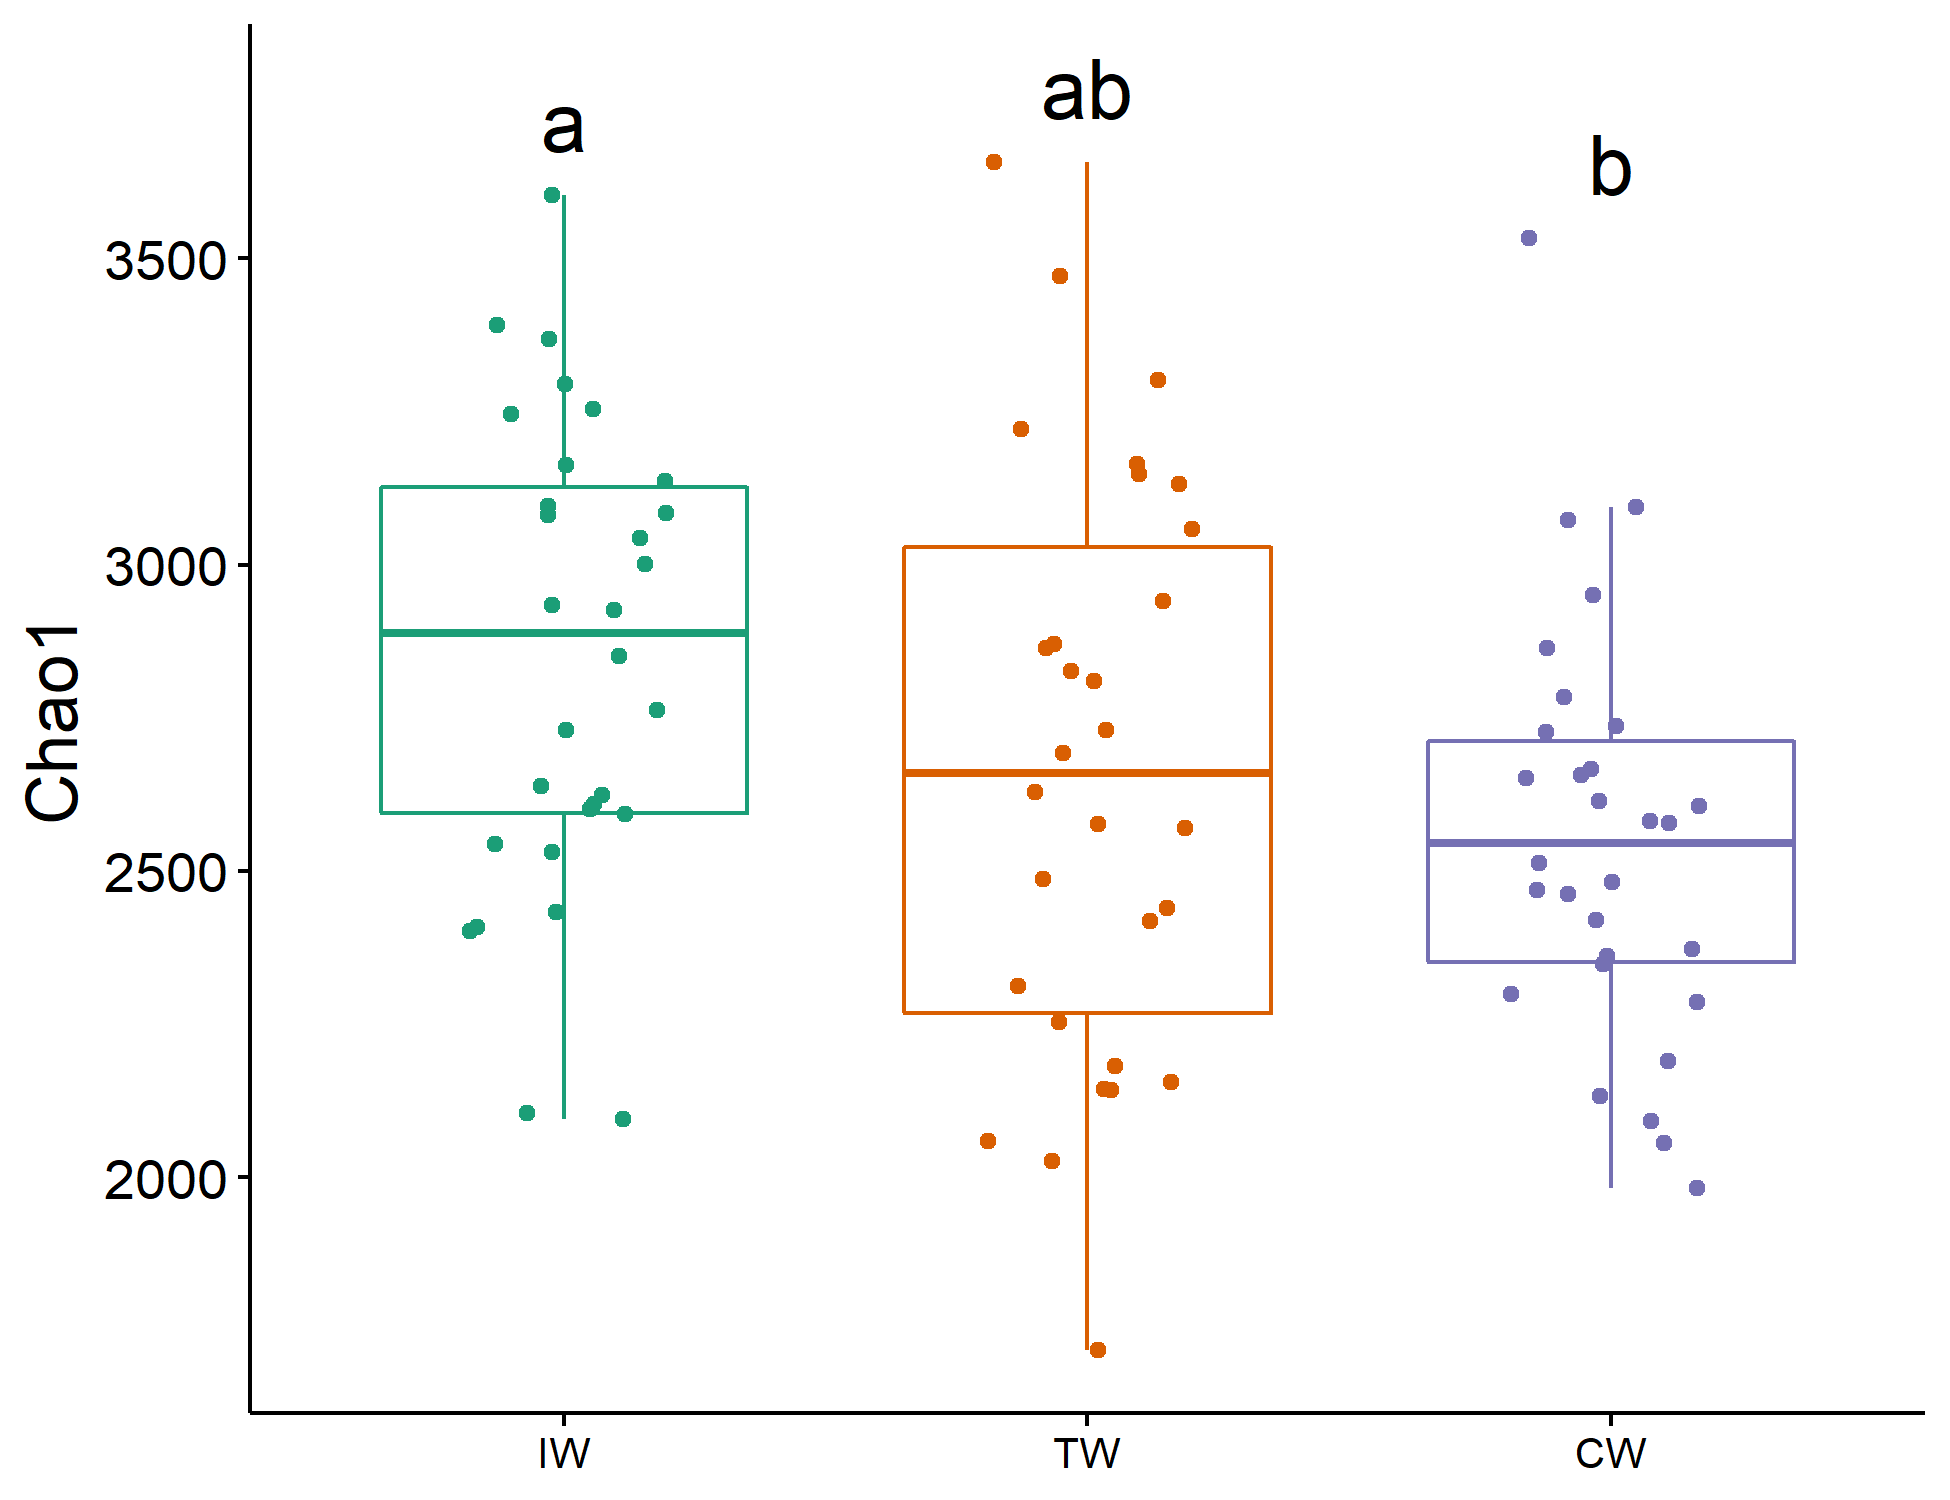
\includegraphics[width=600px]{Images/plot_alpha_letter} \end{center}

We can also use the boxplot to show the paired comparisons directly.

\begin{Shaded}
\begin{Highlighting}[]
\NormalTok{t1}\SpecialCharTok{$}\FunctionTok{plot\_alpha}\NormalTok{(}\AttributeTok{pair\_compare =} \ConstantTok{TRUE}\NormalTok{, }\AttributeTok{measure =} \StringTok{"Chao1"}\NormalTok{, }\AttributeTok{shape =} \StringTok{"Group"}\NormalTok{)}
\end{Highlighting}
\end{Shaded}

\begin{center}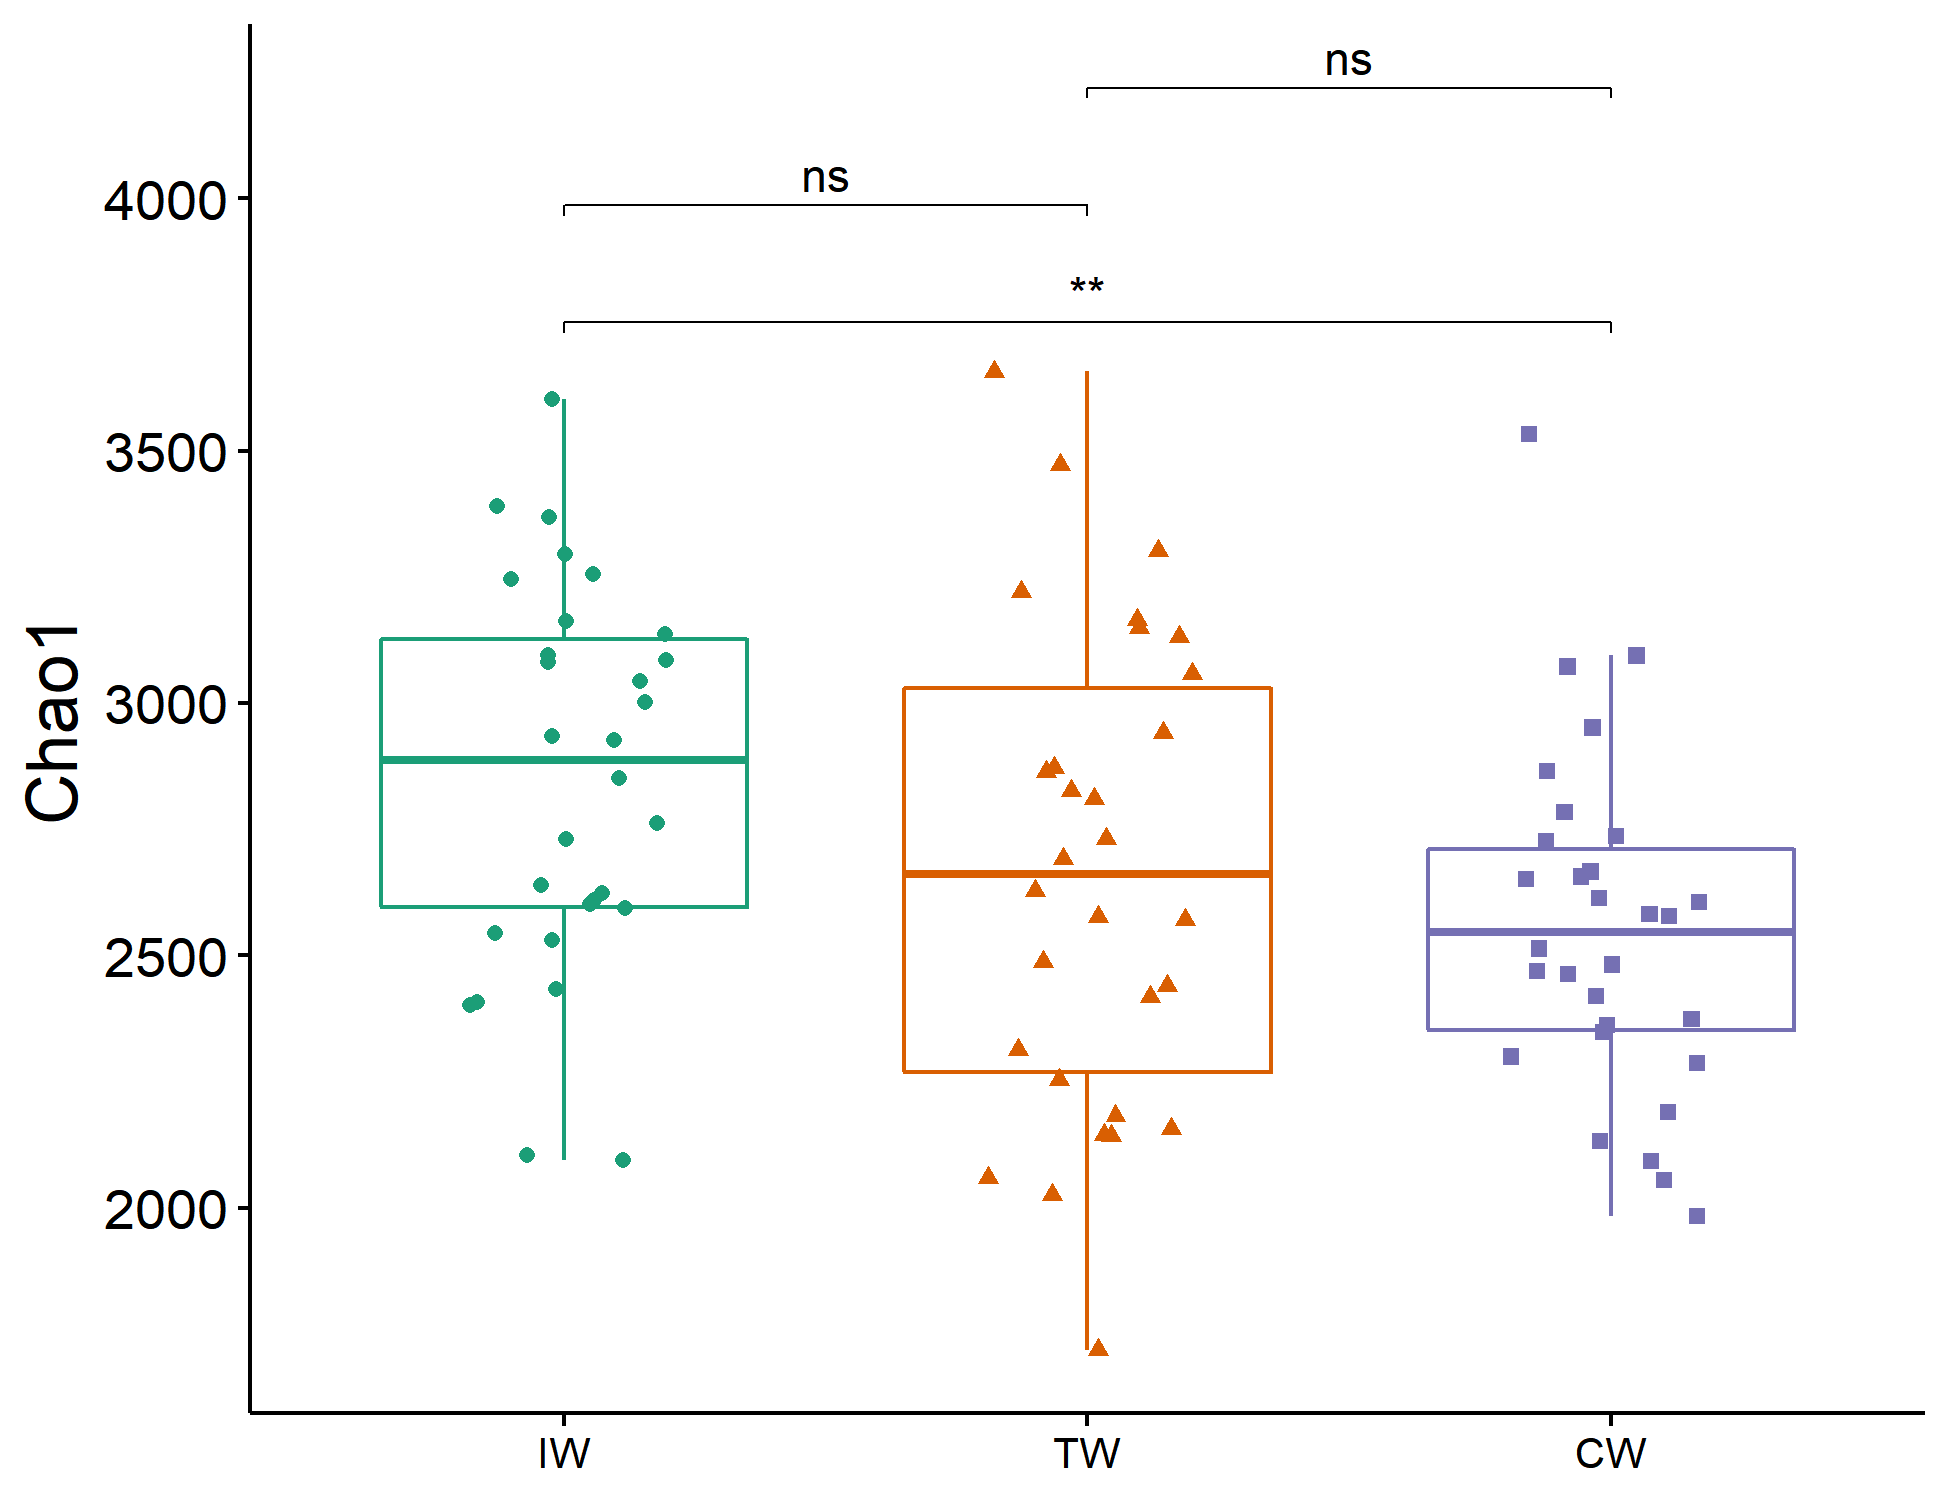
\includegraphics[width=600px]{Images/plot_alpha} \end{center}

\hypertarget{trans_beta-class}{%
\section{trans\_beta class}\label{trans_beta-class}}

 The distance matrix of beta diversity can be transformed and plotted using trans\_beta class.
The analysis referred to the beta diversity in this class mainly include ordination, group distance, clustering and manova.
We first show the ordination using PCoA.

\begin{Shaded}
\begin{Highlighting}[]
\CommentTok{\# we first create an trans\_beta object}
\CommentTok{\# this operation invoke the distance matrix of bray in dataset$beta\_diversity}
\NormalTok{t1 }\OtherTok{\textless{}{-}}\NormalTok{ trans\_beta}\SpecialCharTok{$}\FunctionTok{new}\NormalTok{(}\AttributeTok{dataset =}\NormalTok{ dataset, }\AttributeTok{group =} \StringTok{"Group"}\NormalTok{, }\AttributeTok{measure =} \StringTok{"bray"}\NormalTok{)}
\end{Highlighting}
\end{Shaded}

\begin{verbatim}
## Please also cite the original paper: An et al. (2019). Soil bacterial community structure in Chinese wetlands. Geoderma, 337, 290-299.
\end{verbatim}

\begin{Shaded}
\begin{Highlighting}[]
\NormalTok{t1}\SpecialCharTok{$}\FunctionTok{cal\_ordination}\NormalTok{(}\AttributeTok{ordination =} \StringTok{"PCoA"}\NormalTok{)}
\CommentTok{\# t1$res\_ordination is the ordination result list}
\FunctionTok{class}\NormalTok{(t1}\SpecialCharTok{$}\NormalTok{res\_ordination)}
\CommentTok{\# plot the PCoA result}
\NormalTok{t1}\SpecialCharTok{$}\FunctionTok{plot\_ordination}\NormalTok{(}\AttributeTok{plot\_color =} \StringTok{"Group"}\NormalTok{, }\AttributeTok{plot\_shape =} \StringTok{"Group"}\NormalTok{, }\AttributeTok{plot\_group\_ellipse =} \ConstantTok{TRUE}\NormalTok{)}
\end{Highlighting}
\end{Shaded}

\begin{center}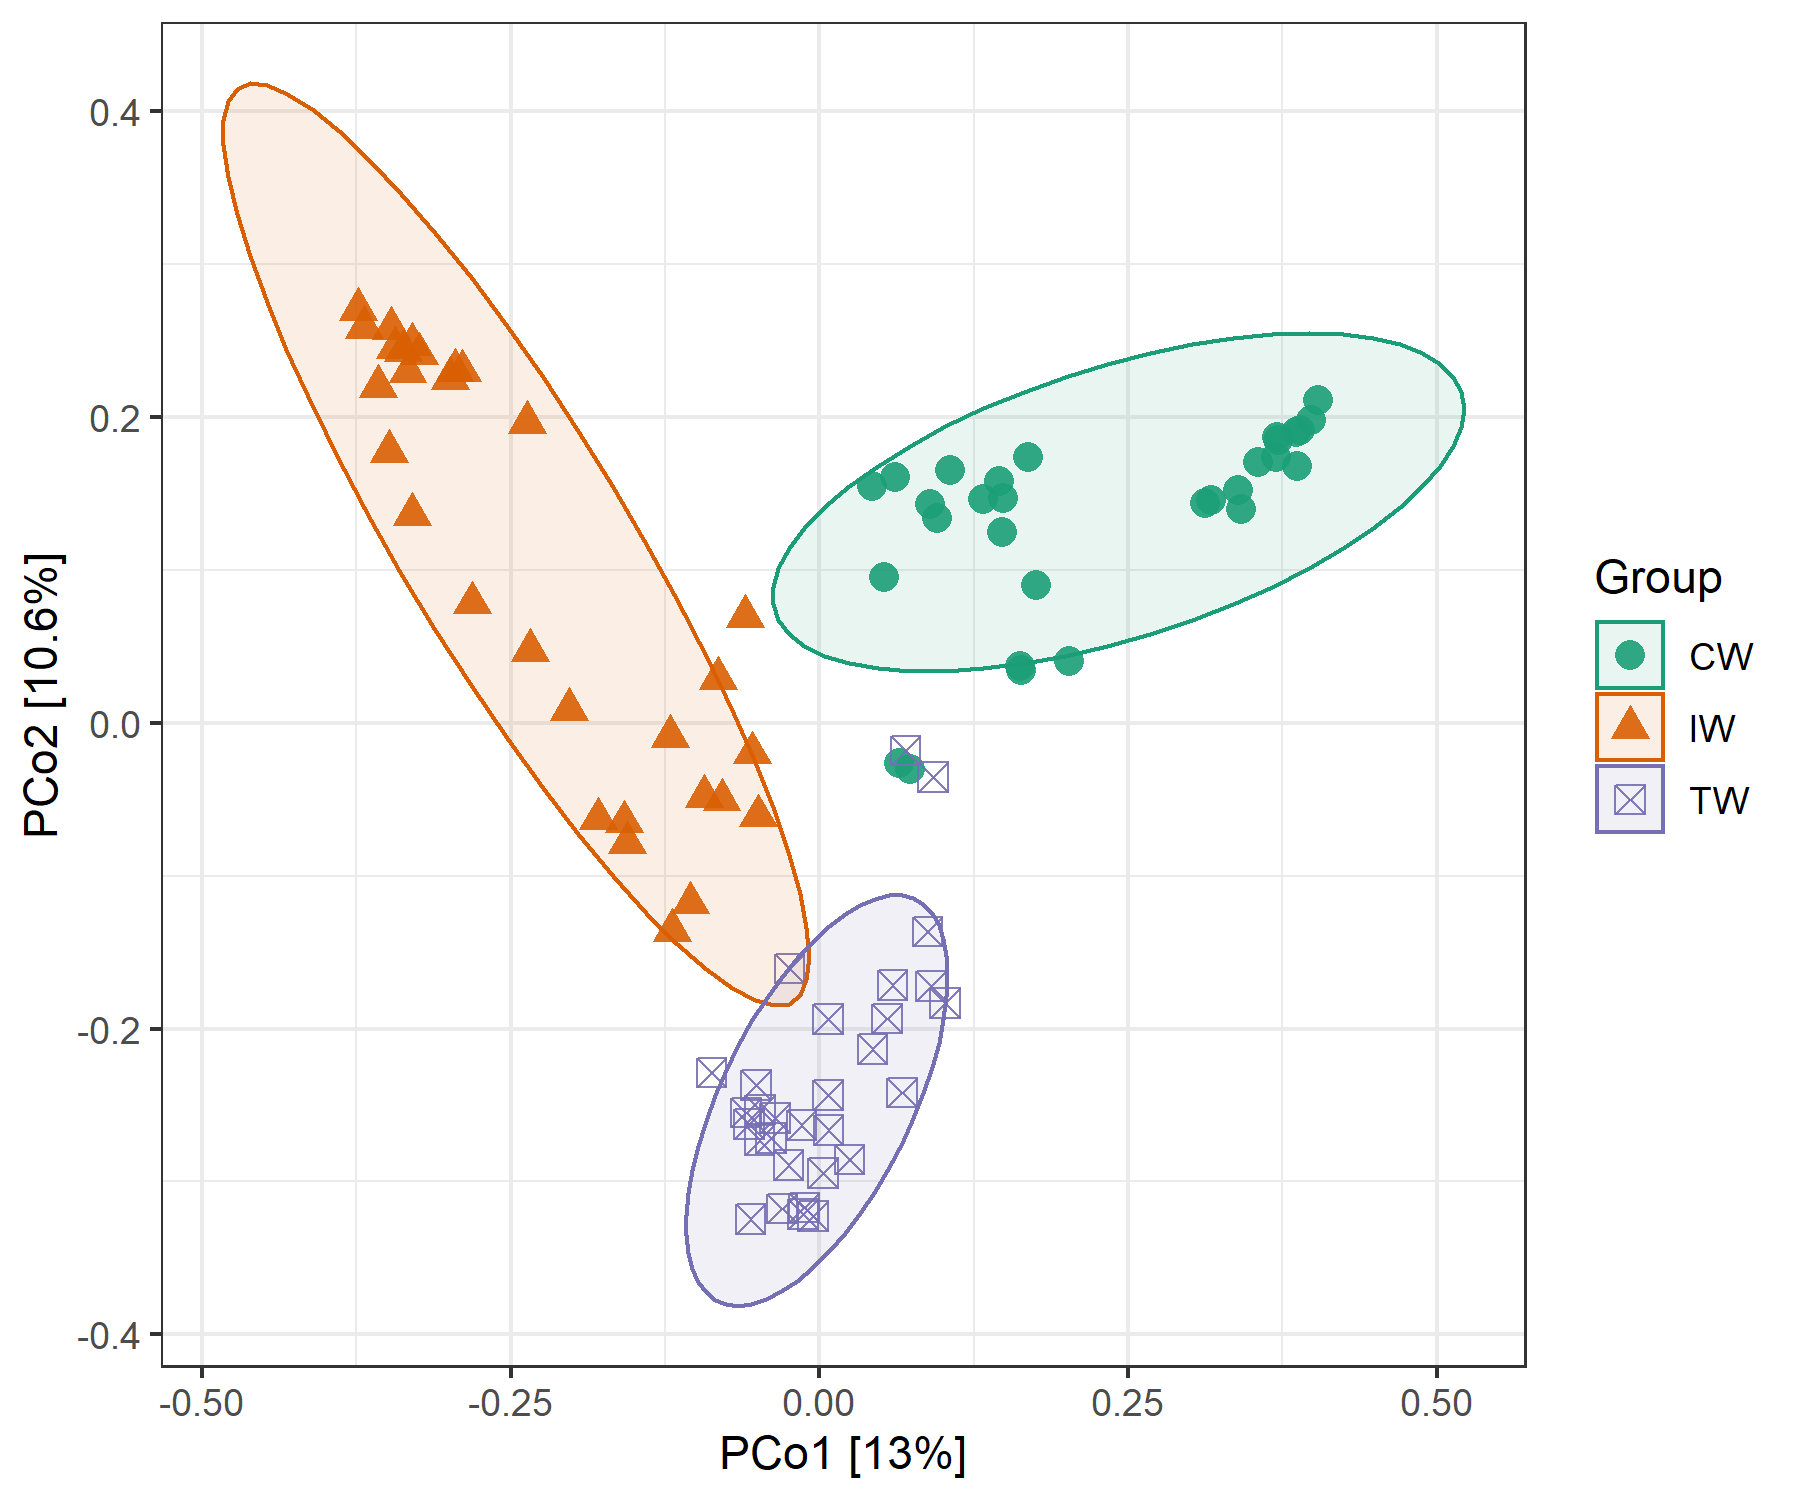
\includegraphics[width=650px]{Images/plot_ordination} \end{center}

Then we plot and compare the group distances.

\begin{Shaded}
\begin{Highlighting}[]
\CommentTok{\# calculate and plot sample distances within groups}
\NormalTok{t1}\SpecialCharTok{$}\FunctionTok{cal\_group\_distance}\NormalTok{()}
\CommentTok{\# return t1$res\_group\_distance}
\NormalTok{t1}\SpecialCharTok{$}\FunctionTok{plot\_group\_distance}\NormalTok{(}\AttributeTok{distance\_pair\_stat =} \ConstantTok{TRUE}\NormalTok{)}
\end{Highlighting}
\end{Shaded}

\begin{center}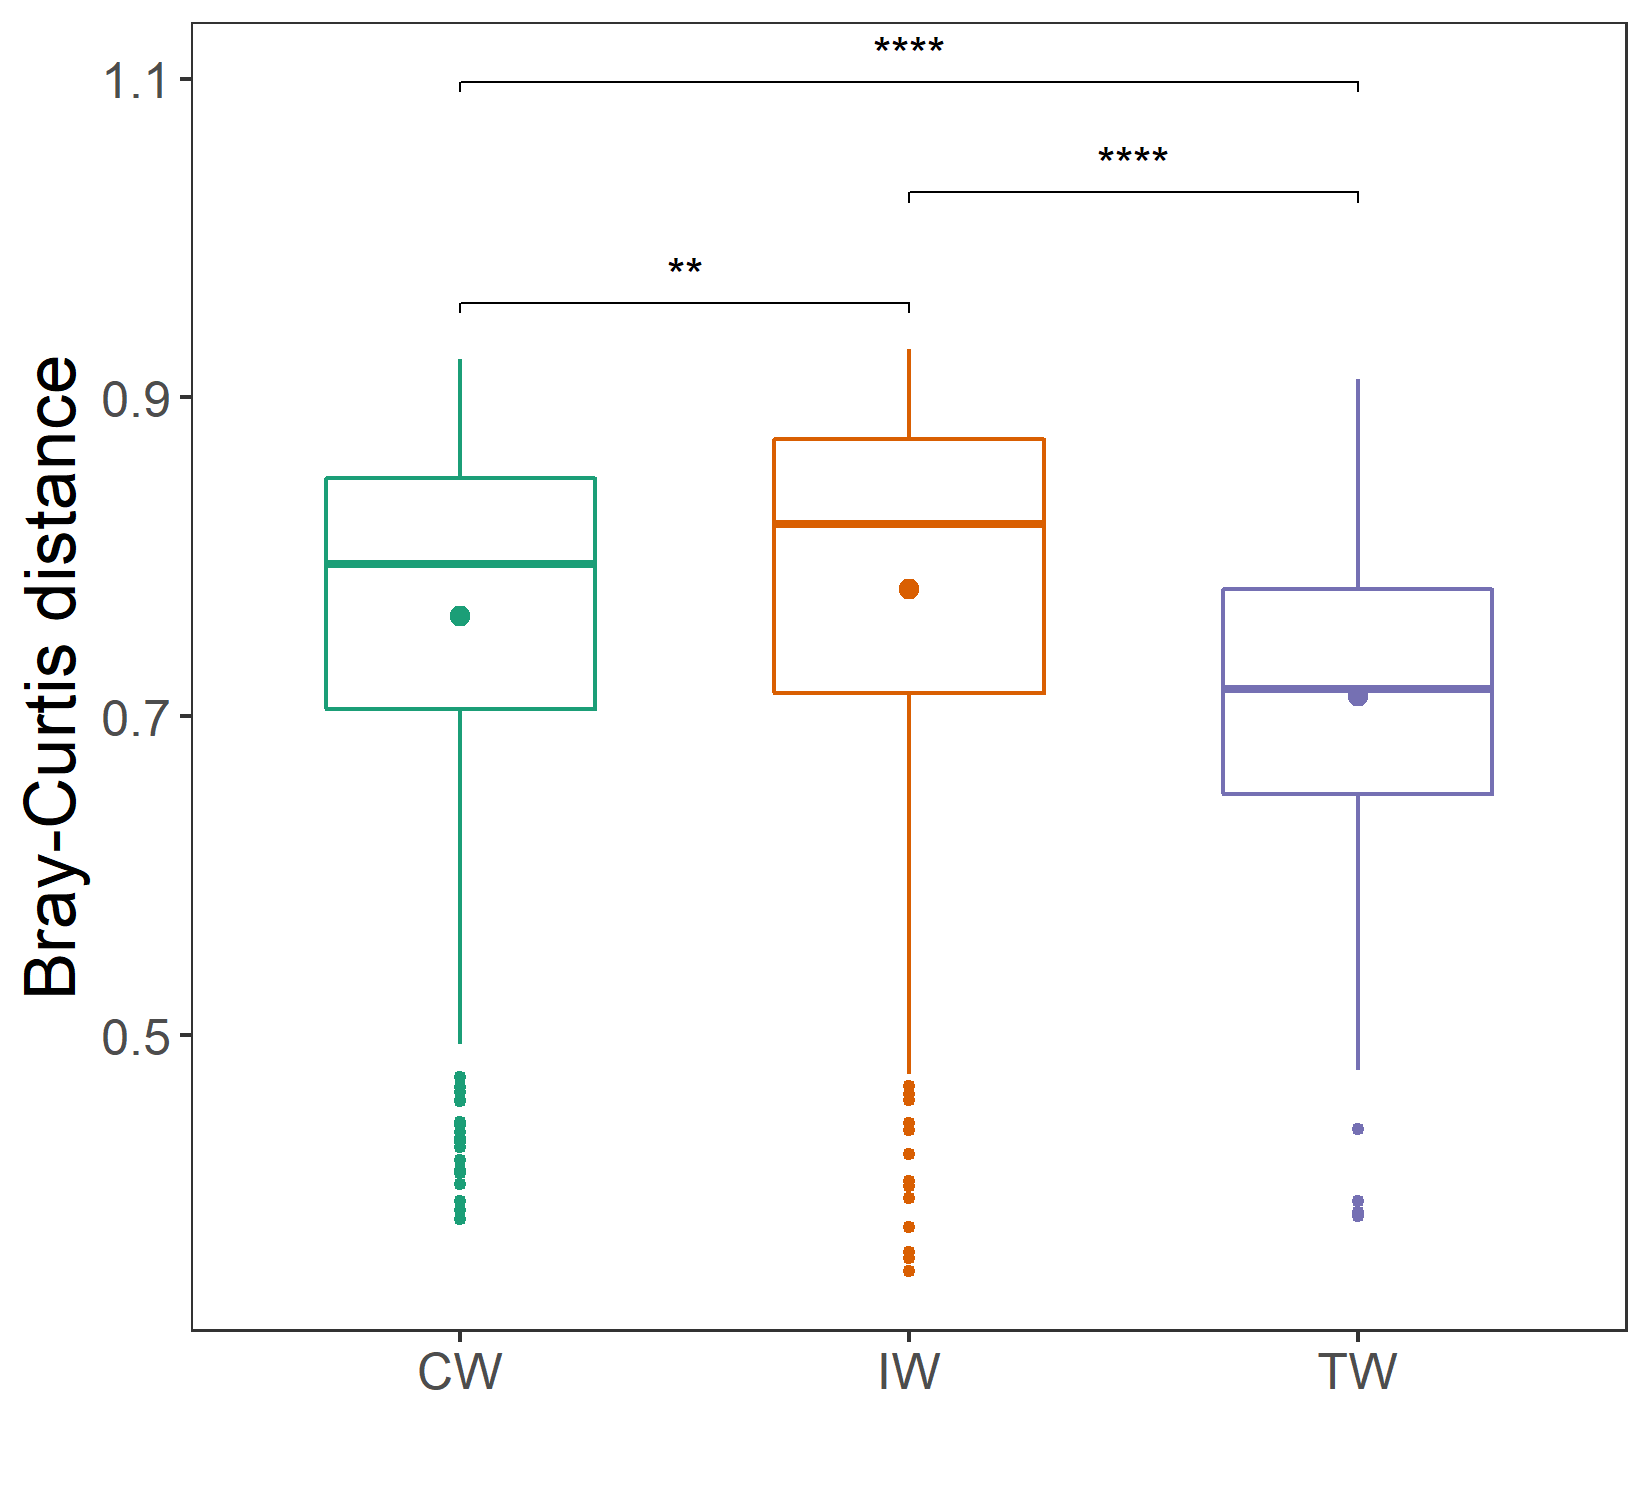
\includegraphics[width=500px]{Images/plot_group_distance_within} \end{center}

\begin{Shaded}
\begin{Highlighting}[]
\CommentTok{\# calculate and plot sample distances between groups}
\NormalTok{t1}\SpecialCharTok{$}\FunctionTok{cal\_group\_distance}\NormalTok{(}\AttributeTok{within\_group =} \ConstantTok{FALSE}\NormalTok{)}
\NormalTok{t1}\SpecialCharTok{$}\FunctionTok{plot\_group\_distance}\NormalTok{(}\AttributeTok{distance\_pair\_stat =} \ConstantTok{TRUE}\NormalTok{)}
\end{Highlighting}
\end{Shaded}

\begin{center}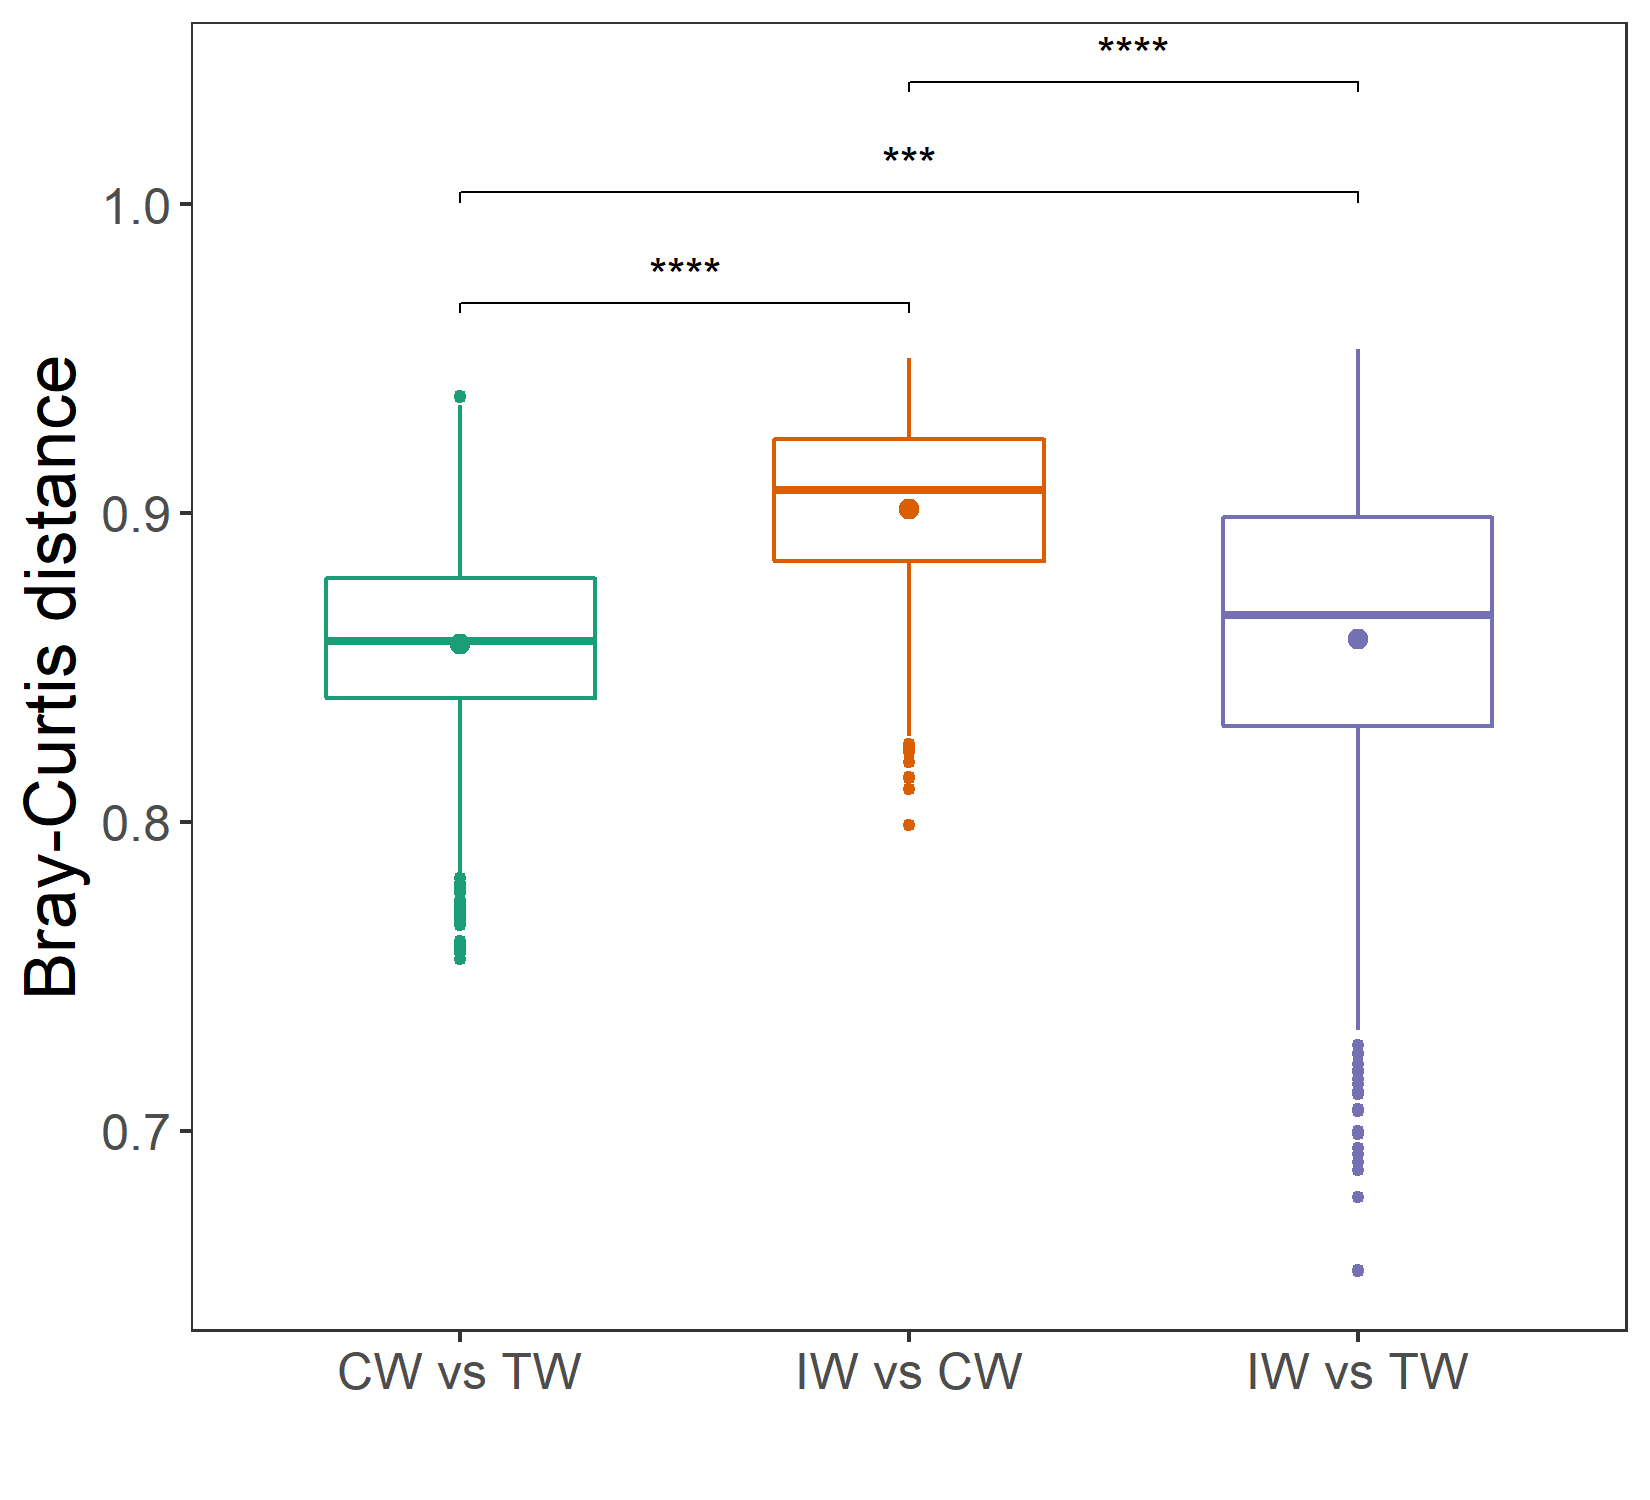
\includegraphics[width=500px]{Images/plot_group_distance_between} \end{center}

Clustering plot is also a frequently used method.

\begin{Shaded}
\begin{Highlighting}[]
\CommentTok{\# use replace\_name to set the label name, group parameter used to set the color}
\NormalTok{t1}\SpecialCharTok{$}\FunctionTok{plot\_clustering}\NormalTok{(}\AttributeTok{group =} \StringTok{"Group"}\NormalTok{, }\AttributeTok{replace\_name =} \FunctionTok{c}\NormalTok{(}\StringTok{"Saline"}\NormalTok{, }\StringTok{"Type"}\NormalTok{))}
\end{Highlighting}
\end{Shaded}

\begin{center}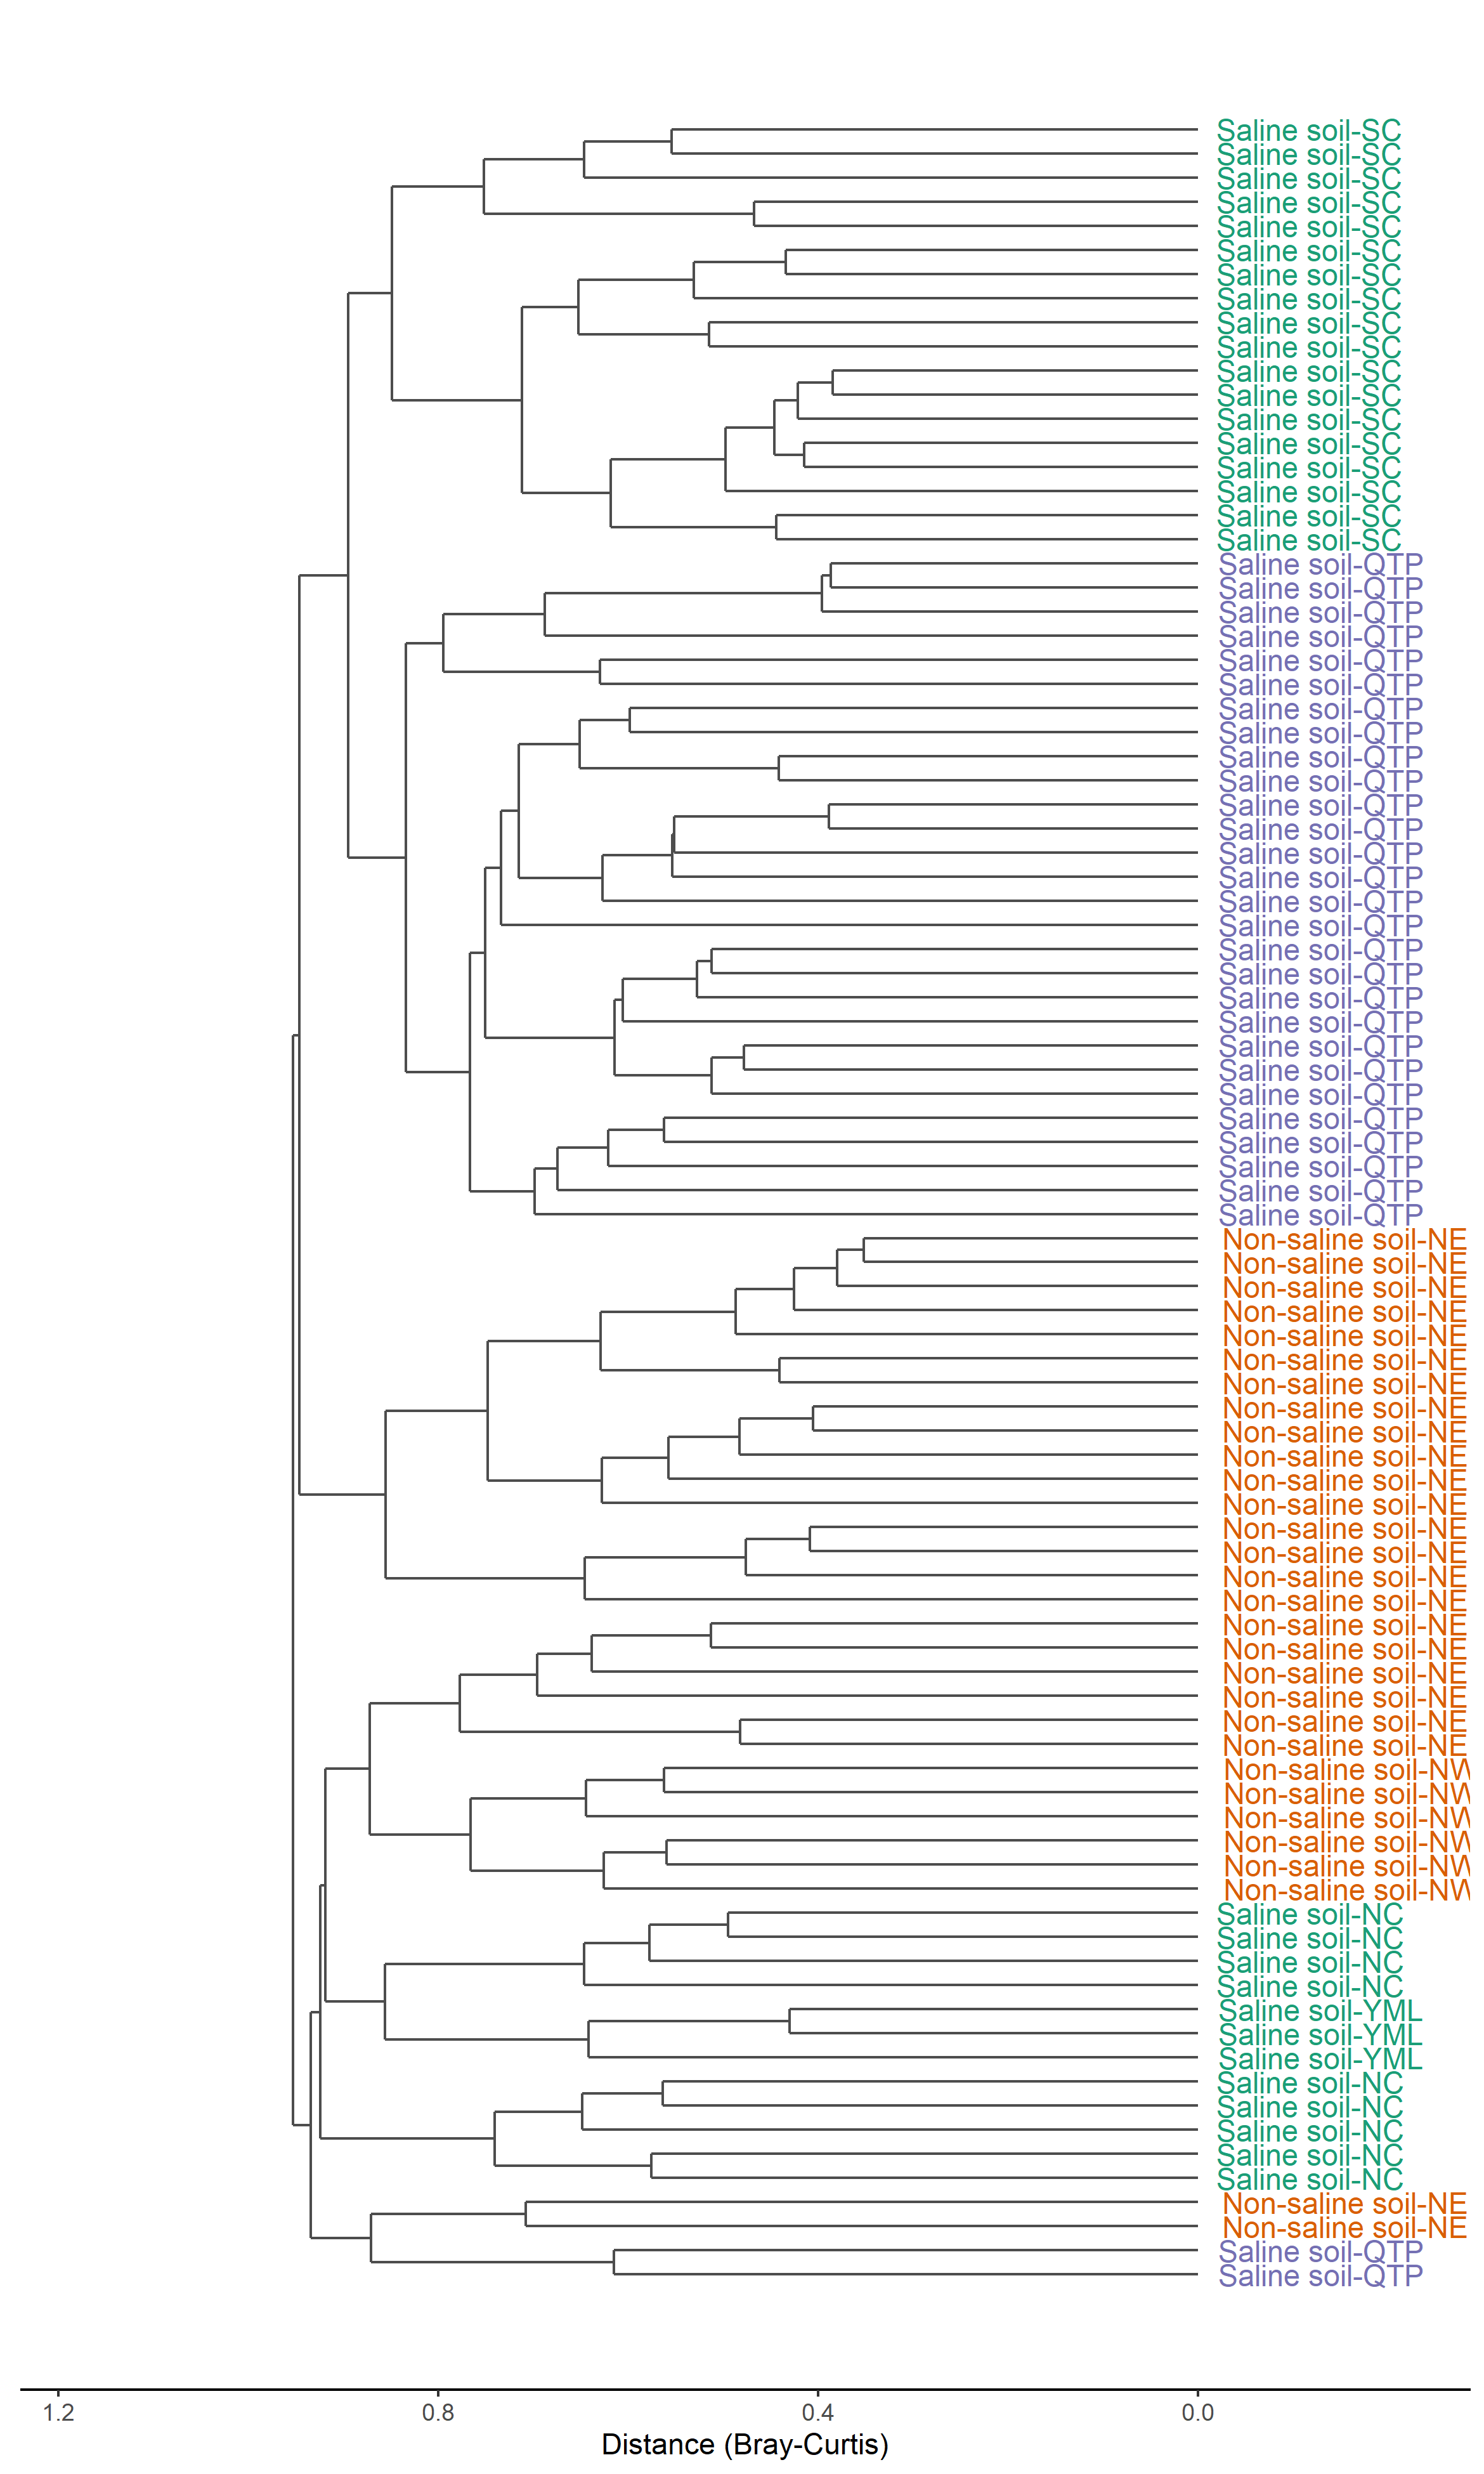
\includegraphics[width=550px]{Images/plot_clustering} \end{center}

perMANOVA\citep{Anderson_Austral_2001} is often used in the differential test of distances among groups.

\begin{Shaded}
\begin{Highlighting}[]
\CommentTok{\# manova for all groups}
\NormalTok{t1}\SpecialCharTok{$}\FunctionTok{cal\_manova}\NormalTok{(}\AttributeTok{cal\_manova\_all =} \ConstantTok{TRUE}\NormalTok{)}
\NormalTok{t1}\SpecialCharTok{$}\NormalTok{res\_manova}\SpecialCharTok{$}\NormalTok{aov.tab}
\end{Highlighting}
\end{Shaded}

\begin{verbatim}
## The result is stored in object$res_manova ...
\end{verbatim}

\begin{longtable}[]{@{}
  >{\centering\arraybackslash}p{(\columnwidth - 12\tabcolsep) * \real{0.22}}
  >{\centering\arraybackslash}p{(\columnwidth - 12\tabcolsep) * \real{0.07}}
  >{\centering\arraybackslash}p{(\columnwidth - 12\tabcolsep) * \real{0.17}}
  >{\centering\arraybackslash}p{(\columnwidth - 12\tabcolsep) * \real{0.14}}
  >{\centering\arraybackslash}p{(\columnwidth - 12\tabcolsep) * \real{0.14}}
  >{\centering\arraybackslash}p{(\columnwidth - 12\tabcolsep) * \real{0.12}}
  >{\centering\arraybackslash}p{(\columnwidth - 12\tabcolsep) * \real{0.12}}@{}}
\caption{Permutation: free}\tabularnewline
\toprule
~ & Df & SumsOfSqs & MeanSqs & F.Model & R2 & Pr(\textgreater F) \\
\midrule
\endfirsthead
\toprule
~ & Df & SumsOfSqs & MeanSqs & F.Model & R2 & Pr(\textgreater F) \\
\midrule
\endhead
\textbf{Group} & 2 & 6.121 & 3.06 & 10.57 & 0.1955 & 0.001 \\
\textbf{Residuals} & 87 & 25.18 & 0.2895 & NA & 0.8045 & NA \\
\textbf{Total} & 89 & 31.3 & NA & NA & 1 & NA \\
\bottomrule
\end{longtable}

\begin{Shaded}
\begin{Highlighting}[]
\CommentTok{\# manova for each paired groups}
\NormalTok{t1}\SpecialCharTok{$}\FunctionTok{cal\_manova}\NormalTok{(}\AttributeTok{cal\_manova\_paired =} \ConstantTok{TRUE}\NormalTok{)}
\NormalTok{t1}\SpecialCharTok{$}\NormalTok{res\_manova}
\end{Highlighting}
\end{Shaded}

\begin{verbatim}
## The result is stored in object$res_manova ...
\end{verbatim}

\begin{longtable}[]{@{}
  >{\centering\arraybackslash}p{(\columnwidth - 10\tabcolsep) * \real{0.15}}
  >{\centering\arraybackslash}p{(\columnwidth - 10\tabcolsep) * \real{0.14}}
  >{\centering\arraybackslash}p{(\columnwidth - 10\tabcolsep) * \real{0.21}}
  >{\centering\arraybackslash}p{(\columnwidth - 10\tabcolsep) * \real{0.12}}
  >{\centering\arraybackslash}p{(\columnwidth - 10\tabcolsep) * \real{0.14}}
  >{\centering\arraybackslash}p{(\columnwidth - 10\tabcolsep) * \real{0.21}}@{}}
\toprule
Groups & measure & permutations & R2 & p.value & Significance \\
\midrule
\endhead
IW vs CW & bray & 999 & 0.1595 & 0.001 & *** \\
IW vs TW & bray & 999 & 0.147 & 0.001 & *** \\
CW vs TW & bray & 999 & 0.1556 & 0.001 & *** \\
\bottomrule
\end{longtable}

\begin{Shaded}
\begin{Highlighting}[]
\CommentTok{\# manova for specified group set: here "Group + Type"}
\NormalTok{t1}\SpecialCharTok{$}\FunctionTok{cal\_manova}\NormalTok{(}\AttributeTok{cal\_manova\_set =} \StringTok{"Group + Type"}\NormalTok{)}
\NormalTok{t1}\SpecialCharTok{$}\NormalTok{res\_manova}\SpecialCharTok{$}\NormalTok{aov.tab}
\end{Highlighting}
\end{Shaded}

\begin{verbatim}
## The result is stored in object$res_manova ...
\end{verbatim}

\begin{longtable}[]{@{}
  >{\centering\arraybackslash}p{(\columnwidth - 12\tabcolsep) * \real{0.22}}
  >{\centering\arraybackslash}p{(\columnwidth - 12\tabcolsep) * \real{0.07}}
  >{\centering\arraybackslash}p{(\columnwidth - 12\tabcolsep) * \real{0.17}}
  >{\centering\arraybackslash}p{(\columnwidth - 12\tabcolsep) * \real{0.14}}
  >{\centering\arraybackslash}p{(\columnwidth - 12\tabcolsep) * \real{0.14}}
  >{\centering\arraybackslash}p{(\columnwidth - 12\tabcolsep) * \real{0.12}}
  >{\centering\arraybackslash}p{(\columnwidth - 12\tabcolsep) * \real{0.12}}@{}}
\caption{Permutation: free}\tabularnewline
\toprule
~ & Df & SumsOfSqs & MeanSqs & F.Model & R2 & Pr(\textgreater F) \\
\midrule
\endfirsthead
\toprule
~ & Df & SumsOfSqs & MeanSqs & F.Model & R2 & Pr(\textgreater F) \\
\midrule
\endhead
\textbf{Group} & 2 & 6.121 & 3.06 & 12.01 & 0.1955 & 0.001 \\
\textbf{Type} & 3 & 3.783 & 1.261 & 4.949 & 0.1208 & 0.001 \\
\textbf{Residuals} & 84 & 21.4 & 0.2548 & NA & 0.6836 & NA \\
\textbf{Total} & 89 & 31.3 & NA & NA & 1 & NA \\
\bottomrule
\end{longtable}

PERMDISP\citep{Anderson_Navigating_2011} is also implemented to check multivariate homogeneity of groups dispersions (variances).

\begin{Shaded}
\begin{Highlighting}[]
\CommentTok{\# PERMDISP for the whole comparison and for each paired groups}
\NormalTok{t1}\SpecialCharTok{$}\FunctionTok{cal\_betadisper}\NormalTok{()}
\end{Highlighting}
\end{Shaded}

\begin{verbatim}
## The result is stored in object$res_betadisper ...
\end{verbatim}

\begin{Shaded}
\begin{Highlighting}[]
\NormalTok{t1}\SpecialCharTok{$}\NormalTok{res\_betadisper}
\end{Highlighting}
\end{Shaded}

\begin{verbatim}
## 
## Permutation test for homogeneity of multivariate dispersions
## Permutation: free
## Number of permutations: 999
## 
## Response: Distances
##           Df  Sum Sq   Mean Sq      F N.Perm Pr(>F)  
## Groups     2 0.04131 0.0206545 4.1682    999  0.021 *
## Residuals 87 0.43110 0.0049552                       
## ---
## Signif. codes:  0 '***' 0.001 '**' 0.01 '*' 0.05 '.' 0.1 ' ' 1
## 
## Pairwise comparisons:
## (Observed p-value below diagonal, permuted p-value above diagonal)
##           CW        IW    TW
## CW           0.4690000 0.063
## IW 0.4621193           0.005
## TW 0.0566190 0.0050319
\end{verbatim}

\hypertarget{trans_diff-class}{%
\section{trans\_diff class}\label{trans_diff-class}}

 Differential abundance test is a very important part in the microbial community data analysis.
It can be used to find the significant taxa in determining the community differences across groups.
Currently, trans\_diff class have four famous approaches to perform this analysis:
metastat\citep{White_Statistical_2009}, LEfSe\citep{Segata_Metagenomic_2011}, random forest and metagenomeSeq\citep{Paulson_Differential_2013}.
Metastat depends on the permutations and t-test and performs well on the sparse data.
It is used for the comparisons of taxonomic abundance between two groups at any taxonomic level.
LEfSe and random forest in this class is mainly used for the identification of biomarkers including all taxonomic level.
metagenomeSeq method is implemented to find significant species between two groups at species level (OTU/ASV).

\begin{Shaded}
\begin{Highlighting}[]
\CommentTok{\# metastat analysis at Genus level}
\NormalTok{t1 }\OtherTok{\textless{}{-}}\NormalTok{ trans\_diff}\SpecialCharTok{$}\FunctionTok{new}\NormalTok{(}\AttributeTok{dataset =}\NormalTok{ dataset, }\AttributeTok{method =} \StringTok{"metastat"}\NormalTok{, }\AttributeTok{group =} \StringTok{"Group"}\NormalTok{, }\AttributeTok{metastat\_taxa\_level =} \StringTok{"Genus"}\NormalTok{)}
\CommentTok{\# t1$res\_metastat is the result}
\CommentTok{\# t1$res\_metastat\_group\_matrix is the group comparisons order for plotting}
\CommentTok{\# plot the first paired groups, choose\_group = 1}
\NormalTok{t1}\SpecialCharTok{$}\FunctionTok{plot\_metastat}\NormalTok{(}\AttributeTok{use\_number =} \DecValTok{1}\SpecialCharTok{:}\DecValTok{10}\NormalTok{, }\AttributeTok{qvalue =} \FloatTok{0.05}\NormalTok{, }\AttributeTok{choose\_group =} \DecValTok{1}\NormalTok{)}
\end{Highlighting}
\end{Shaded}

\begin{center}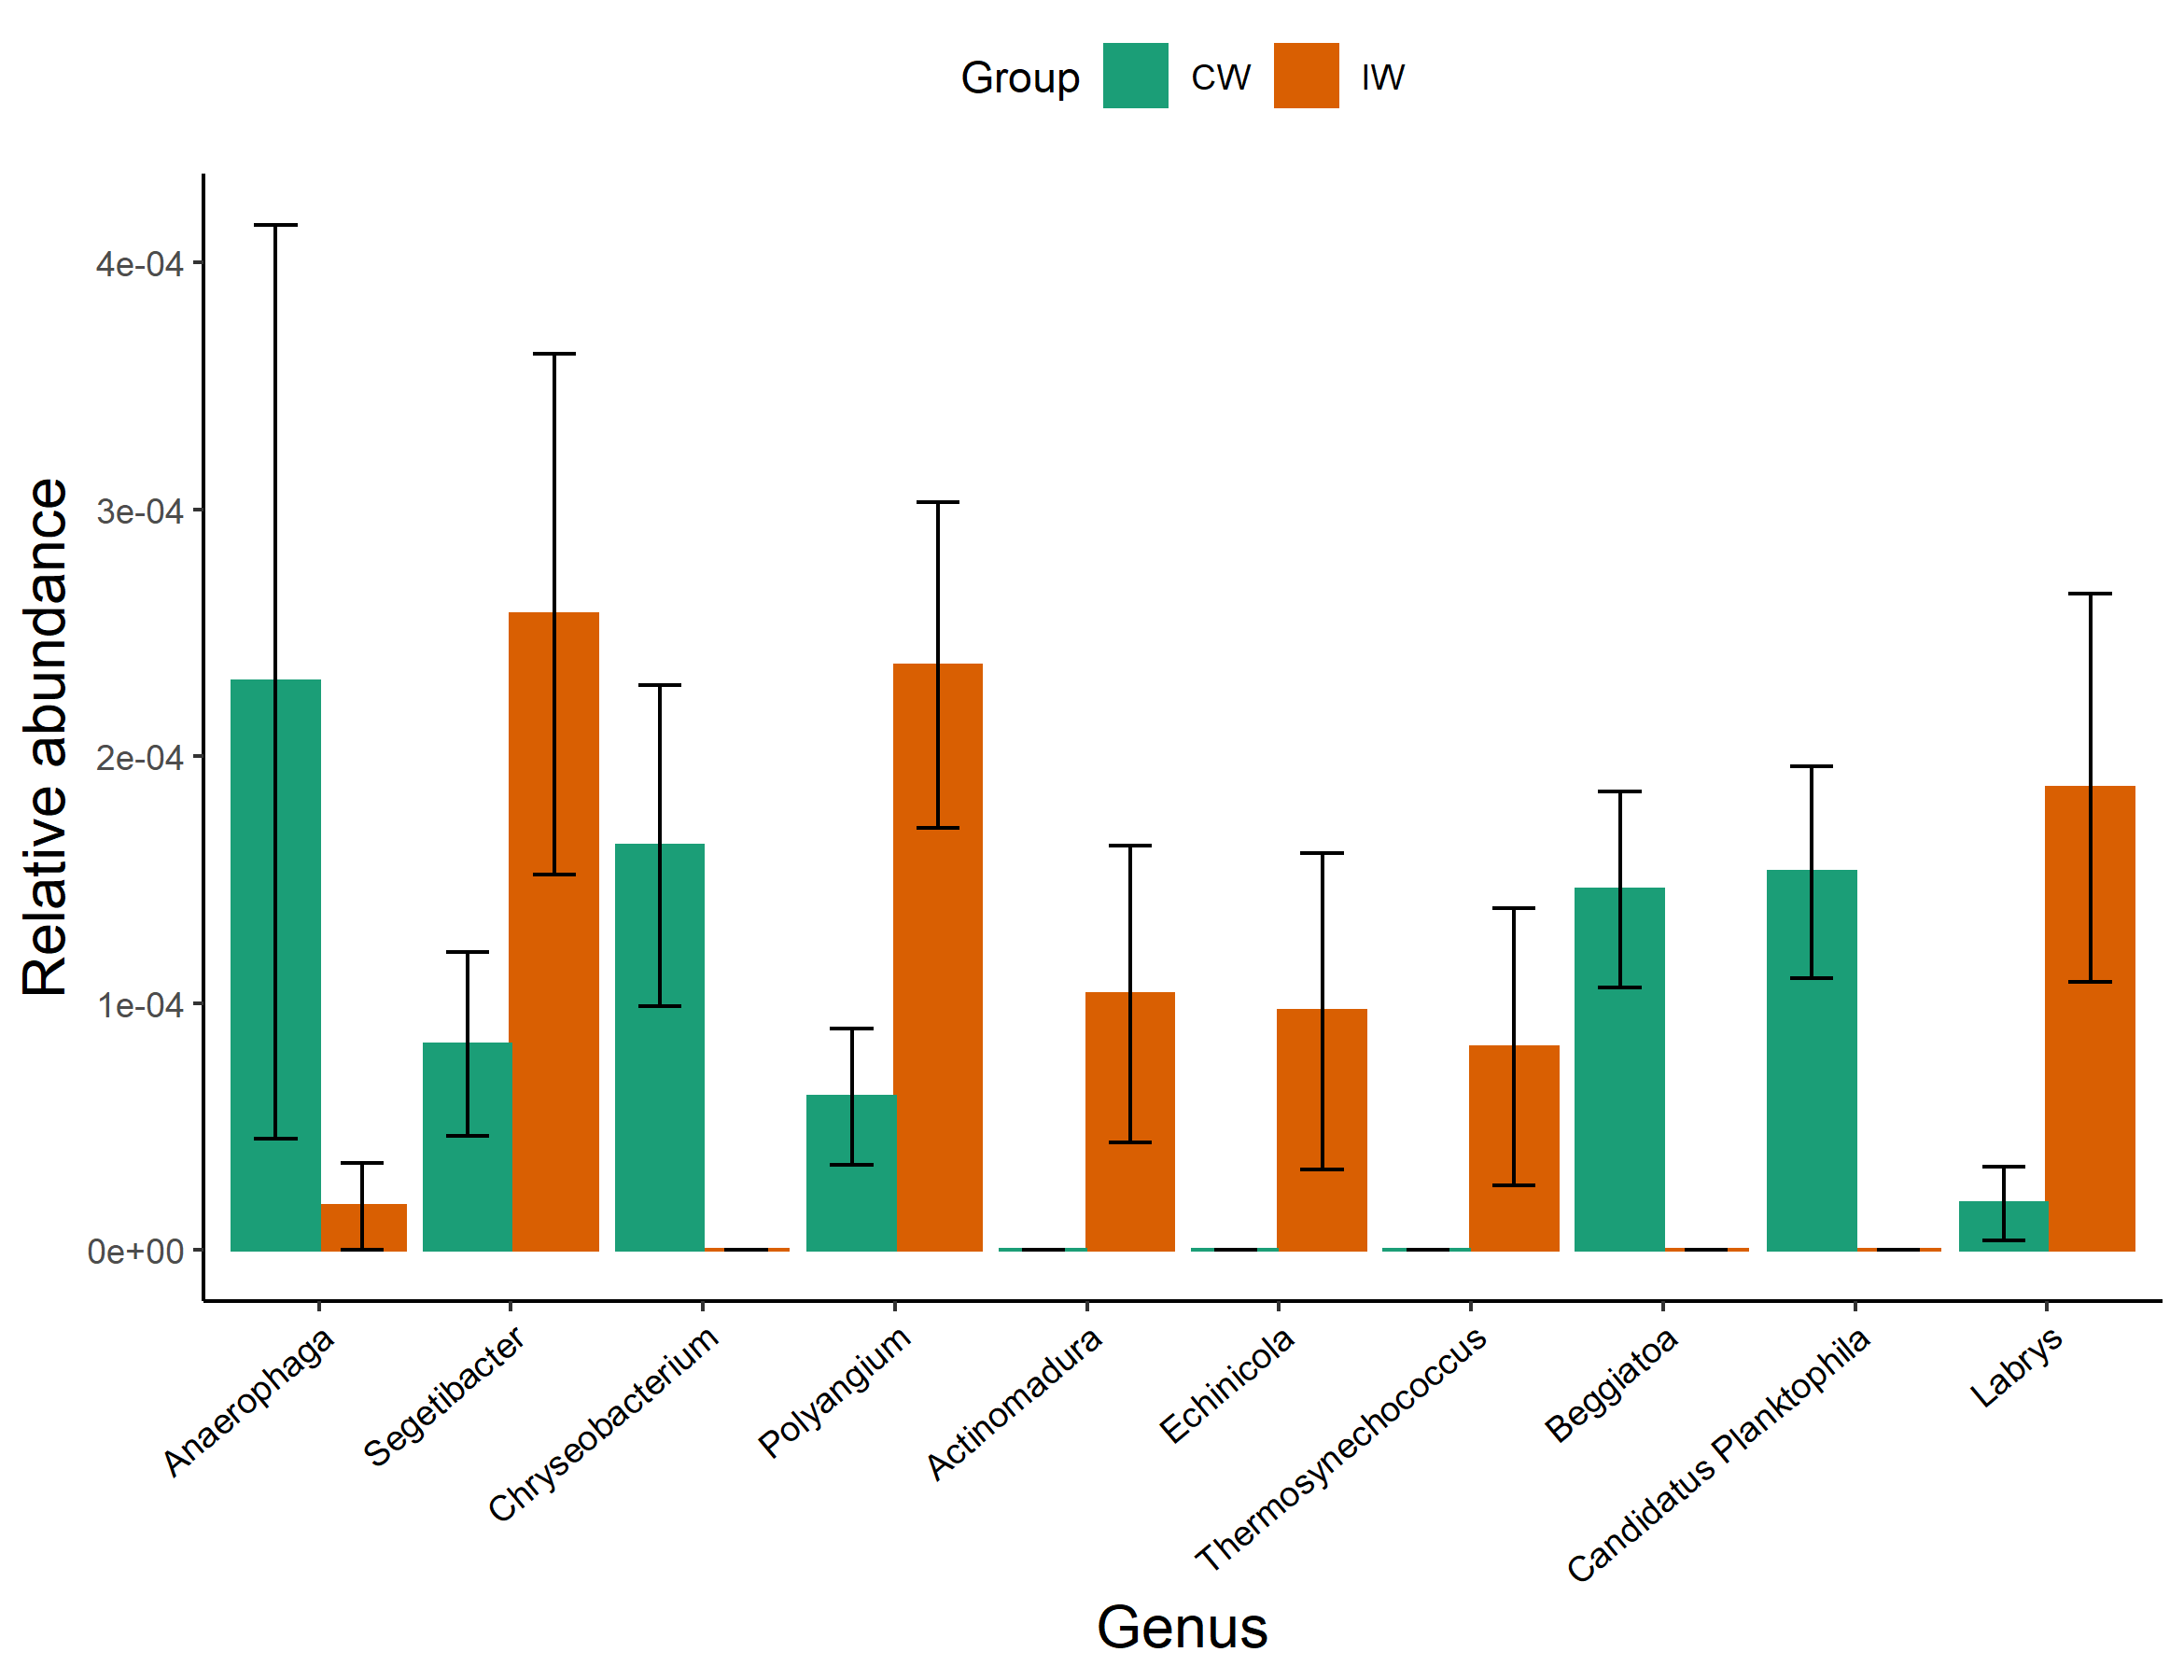
\includegraphics[width=650px]{Images/plot_metastat_1} \end{center}

LEfSe combines the non-parametric test and linear discriminant analysis.
We implement this approach in this package instead of the python version.

\begin{Shaded}
\begin{Highlighting}[]
\NormalTok{t1 }\OtherTok{\textless{}{-}}\NormalTok{ trans\_diff}\SpecialCharTok{$}\FunctionTok{new}\NormalTok{(}\AttributeTok{dataset =}\NormalTok{ dataset, }\AttributeTok{method =} \StringTok{"lefse"}\NormalTok{, }\AttributeTok{group =} \StringTok{"Group"}\NormalTok{, }\AttributeTok{alpha =} \FloatTok{0.01}\NormalTok{, }\AttributeTok{lefse\_subgroup =} \ConstantTok{NULL}\NormalTok{)}
\CommentTok{\# t1$res\_lefse is the LEfSe result}
\CommentTok{\# t1$res\_abund is the abundance information}
\NormalTok{t1}\SpecialCharTok{$}\FunctionTok{plot\_lefse\_bar}\NormalTok{(}\AttributeTok{LDA\_score =} \DecValTok{4}\NormalTok{)}
\end{Highlighting}
\end{Shaded}

\begin{center}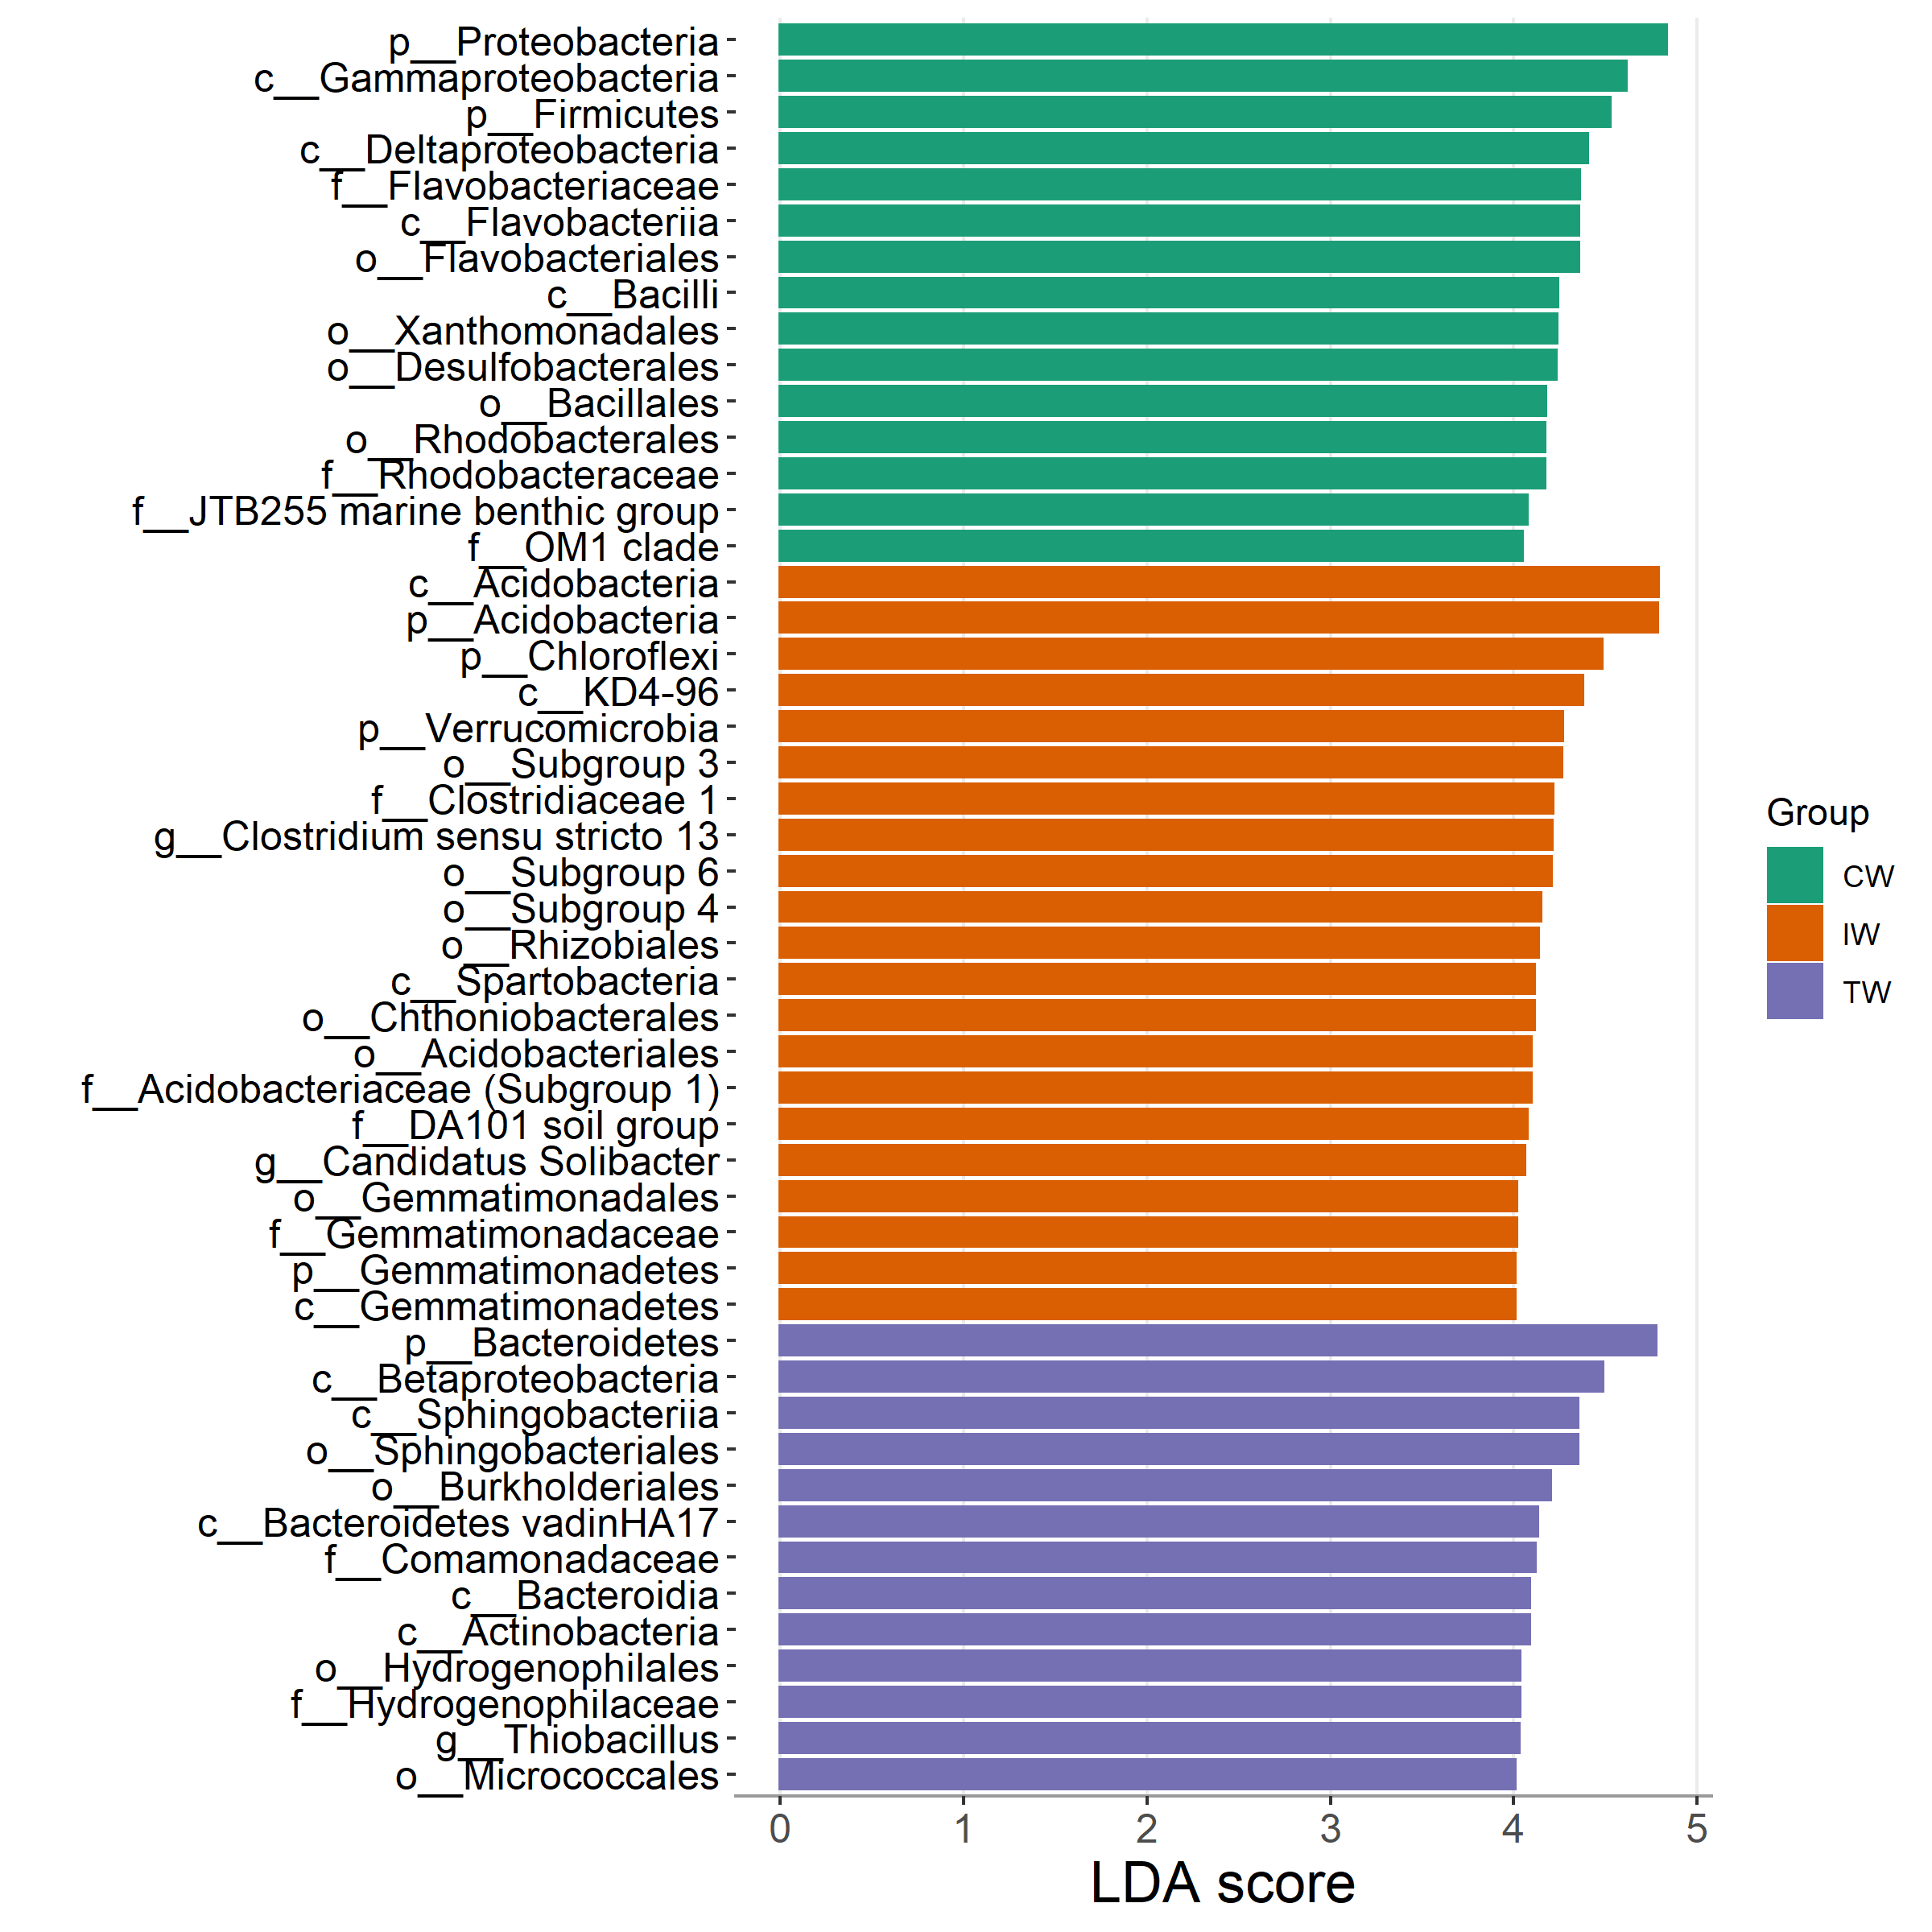
\includegraphics[width=700px]{Images/plot_lefse_bar} \end{center}

\begin{Shaded}
\begin{Highlighting}[]
\NormalTok{t1}\SpecialCharTok{$}\NormalTok{res\_lefse[}\DecValTok{1}\SpecialCharTok{:}\DecValTok{5}\NormalTok{, ]}
\end{Highlighting}
\end{Shaded}

\begin{longtable}[]{@{}
  >{\centering\arraybackslash}p{(\columnwidth - 6\tabcolsep) * \real{0.66}}
  >{\centering\arraybackslash}p{(\columnwidth - 6\tabcolsep) * \real{0.10}}
  >{\centering\arraybackslash}p{(\columnwidth - 6\tabcolsep) * \real{0.14}}
  >{\centering\arraybackslash}p{(\columnwidth - 6\tabcolsep) * \real{0.10}}@{}}
\toprule
Taxa & Group & pvalue & LDA \\
\midrule
\endhead
k\_\_Bacteria\textbar p\_\_Proteobacteria & CW & 3.21e-11 & 4.834 \\
k\_\_Bacteria\textbar p\_\_Acidobacteria\textbar c\_\_Acidobacteria & IW & 8.559e-13 & 4.787 \\
k\_\_Bacteria\textbar p\_\_Acidobacteria & IW & 5.749e-12 & 4.785 \\
k\_\_Bacteria\textbar p\_\_Bacteroidetes & TW & 1.19e-09 & 4.776 \\
k\_\_Bacteria\textbar p\_\_Proteobacteria\textbar c\_\_Gammaproteobacteria & CW & 5.475e-12 & 4.613 \\
\bottomrule
\end{longtable}

Then, we plot the abundance of biomarkers detected by LEfSe.

\begin{Shaded}
\begin{Highlighting}[]
\NormalTok{t1}\SpecialCharTok{$}\FunctionTok{plot\_diff\_abund}\NormalTok{(}\AttributeTok{use\_number =} \DecValTok{1}\SpecialCharTok{:}\DecValTok{30}\NormalTok{)}
\end{Highlighting}
\end{Shaded}

\begin{center}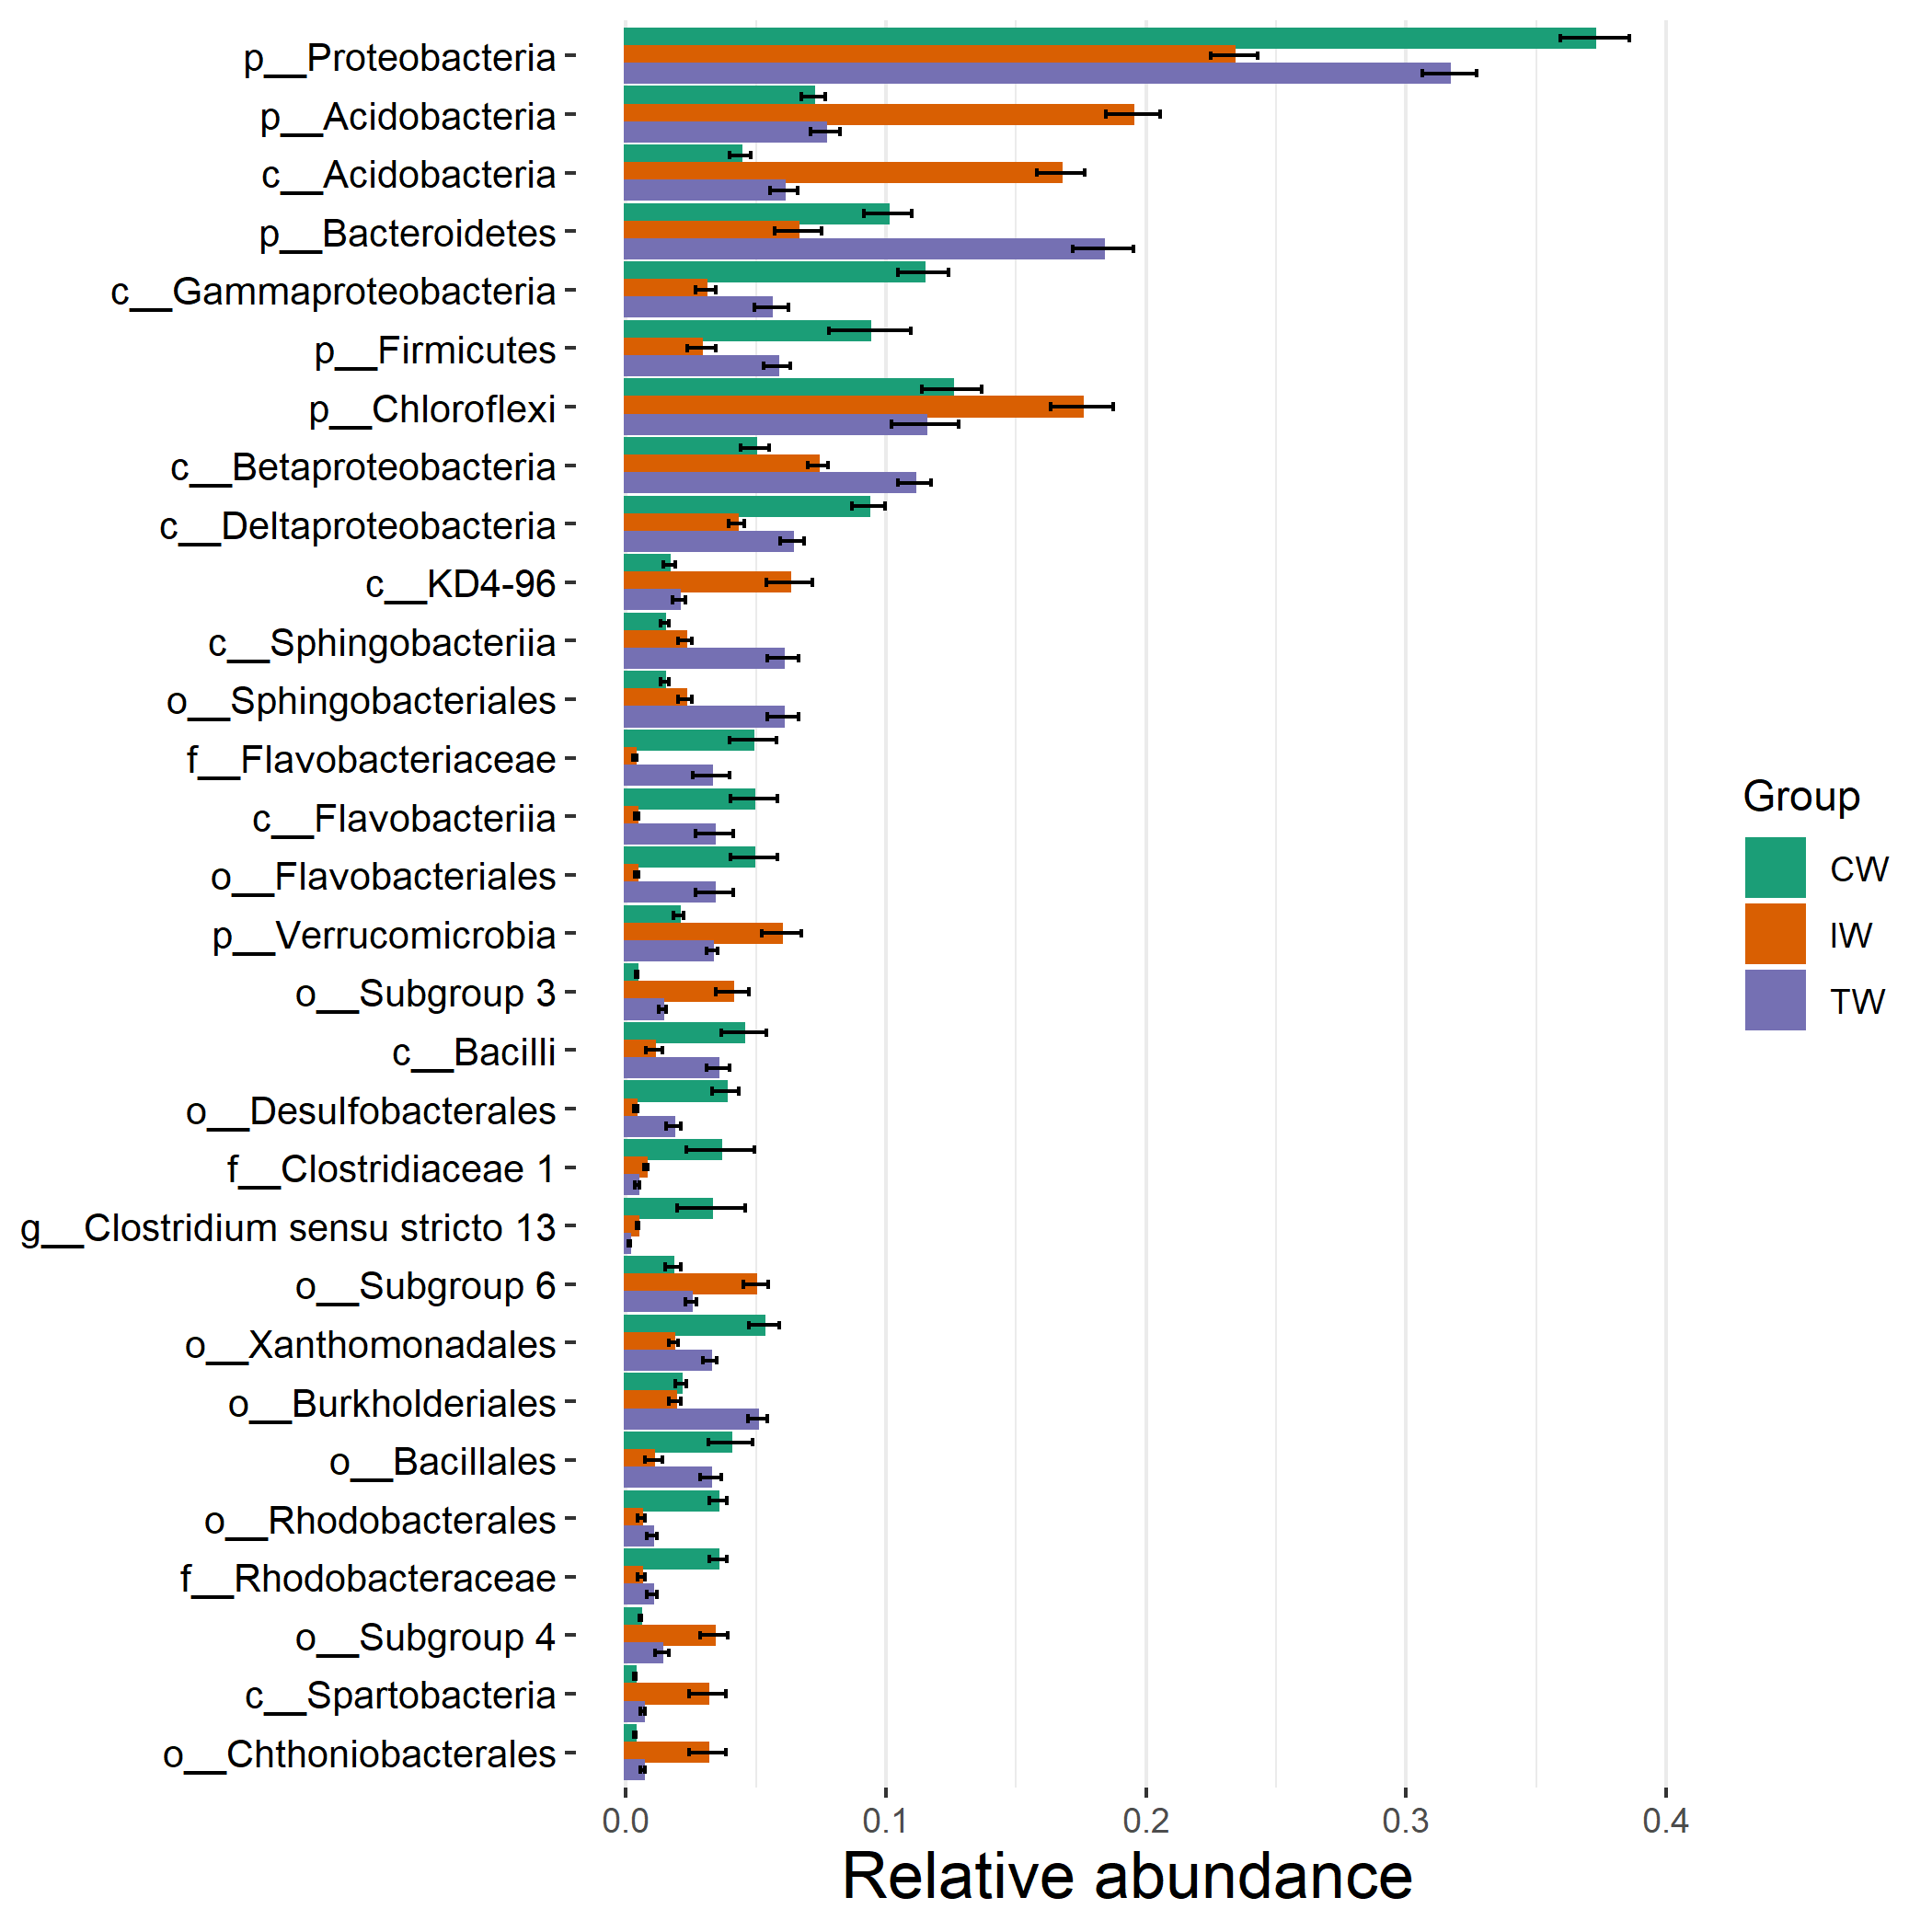
\includegraphics[width=650px]{Images/plot_lefse_diff_abund} \end{center}

Then, we show the cladogram of the differential features in the taxonomic tree.
There are too many taxa in this dataset.
As an example, we only use the highest 200 abundant taxa in the tree and 50 differential features.
We only show the full taxonomic label at Phylum level and use letters at other levels to reduce the text overlap.

\begin{Shaded}
\begin{Highlighting}[]
\CommentTok{\# clade\_label\_level 5 represent phylum level in this analysis}
\CommentTok{\# require ggtree package}
\NormalTok{t1}\SpecialCharTok{$}\FunctionTok{plot\_lefse\_cladogram}\NormalTok{(}\AttributeTok{use\_taxa\_num =} \DecValTok{200}\NormalTok{, }\AttributeTok{use\_feature\_num =} \DecValTok{50}\NormalTok{, }\AttributeTok{clade\_label\_level =} \DecValTok{5}\NormalTok{)}
\end{Highlighting}
\end{Shaded}

\begin{center}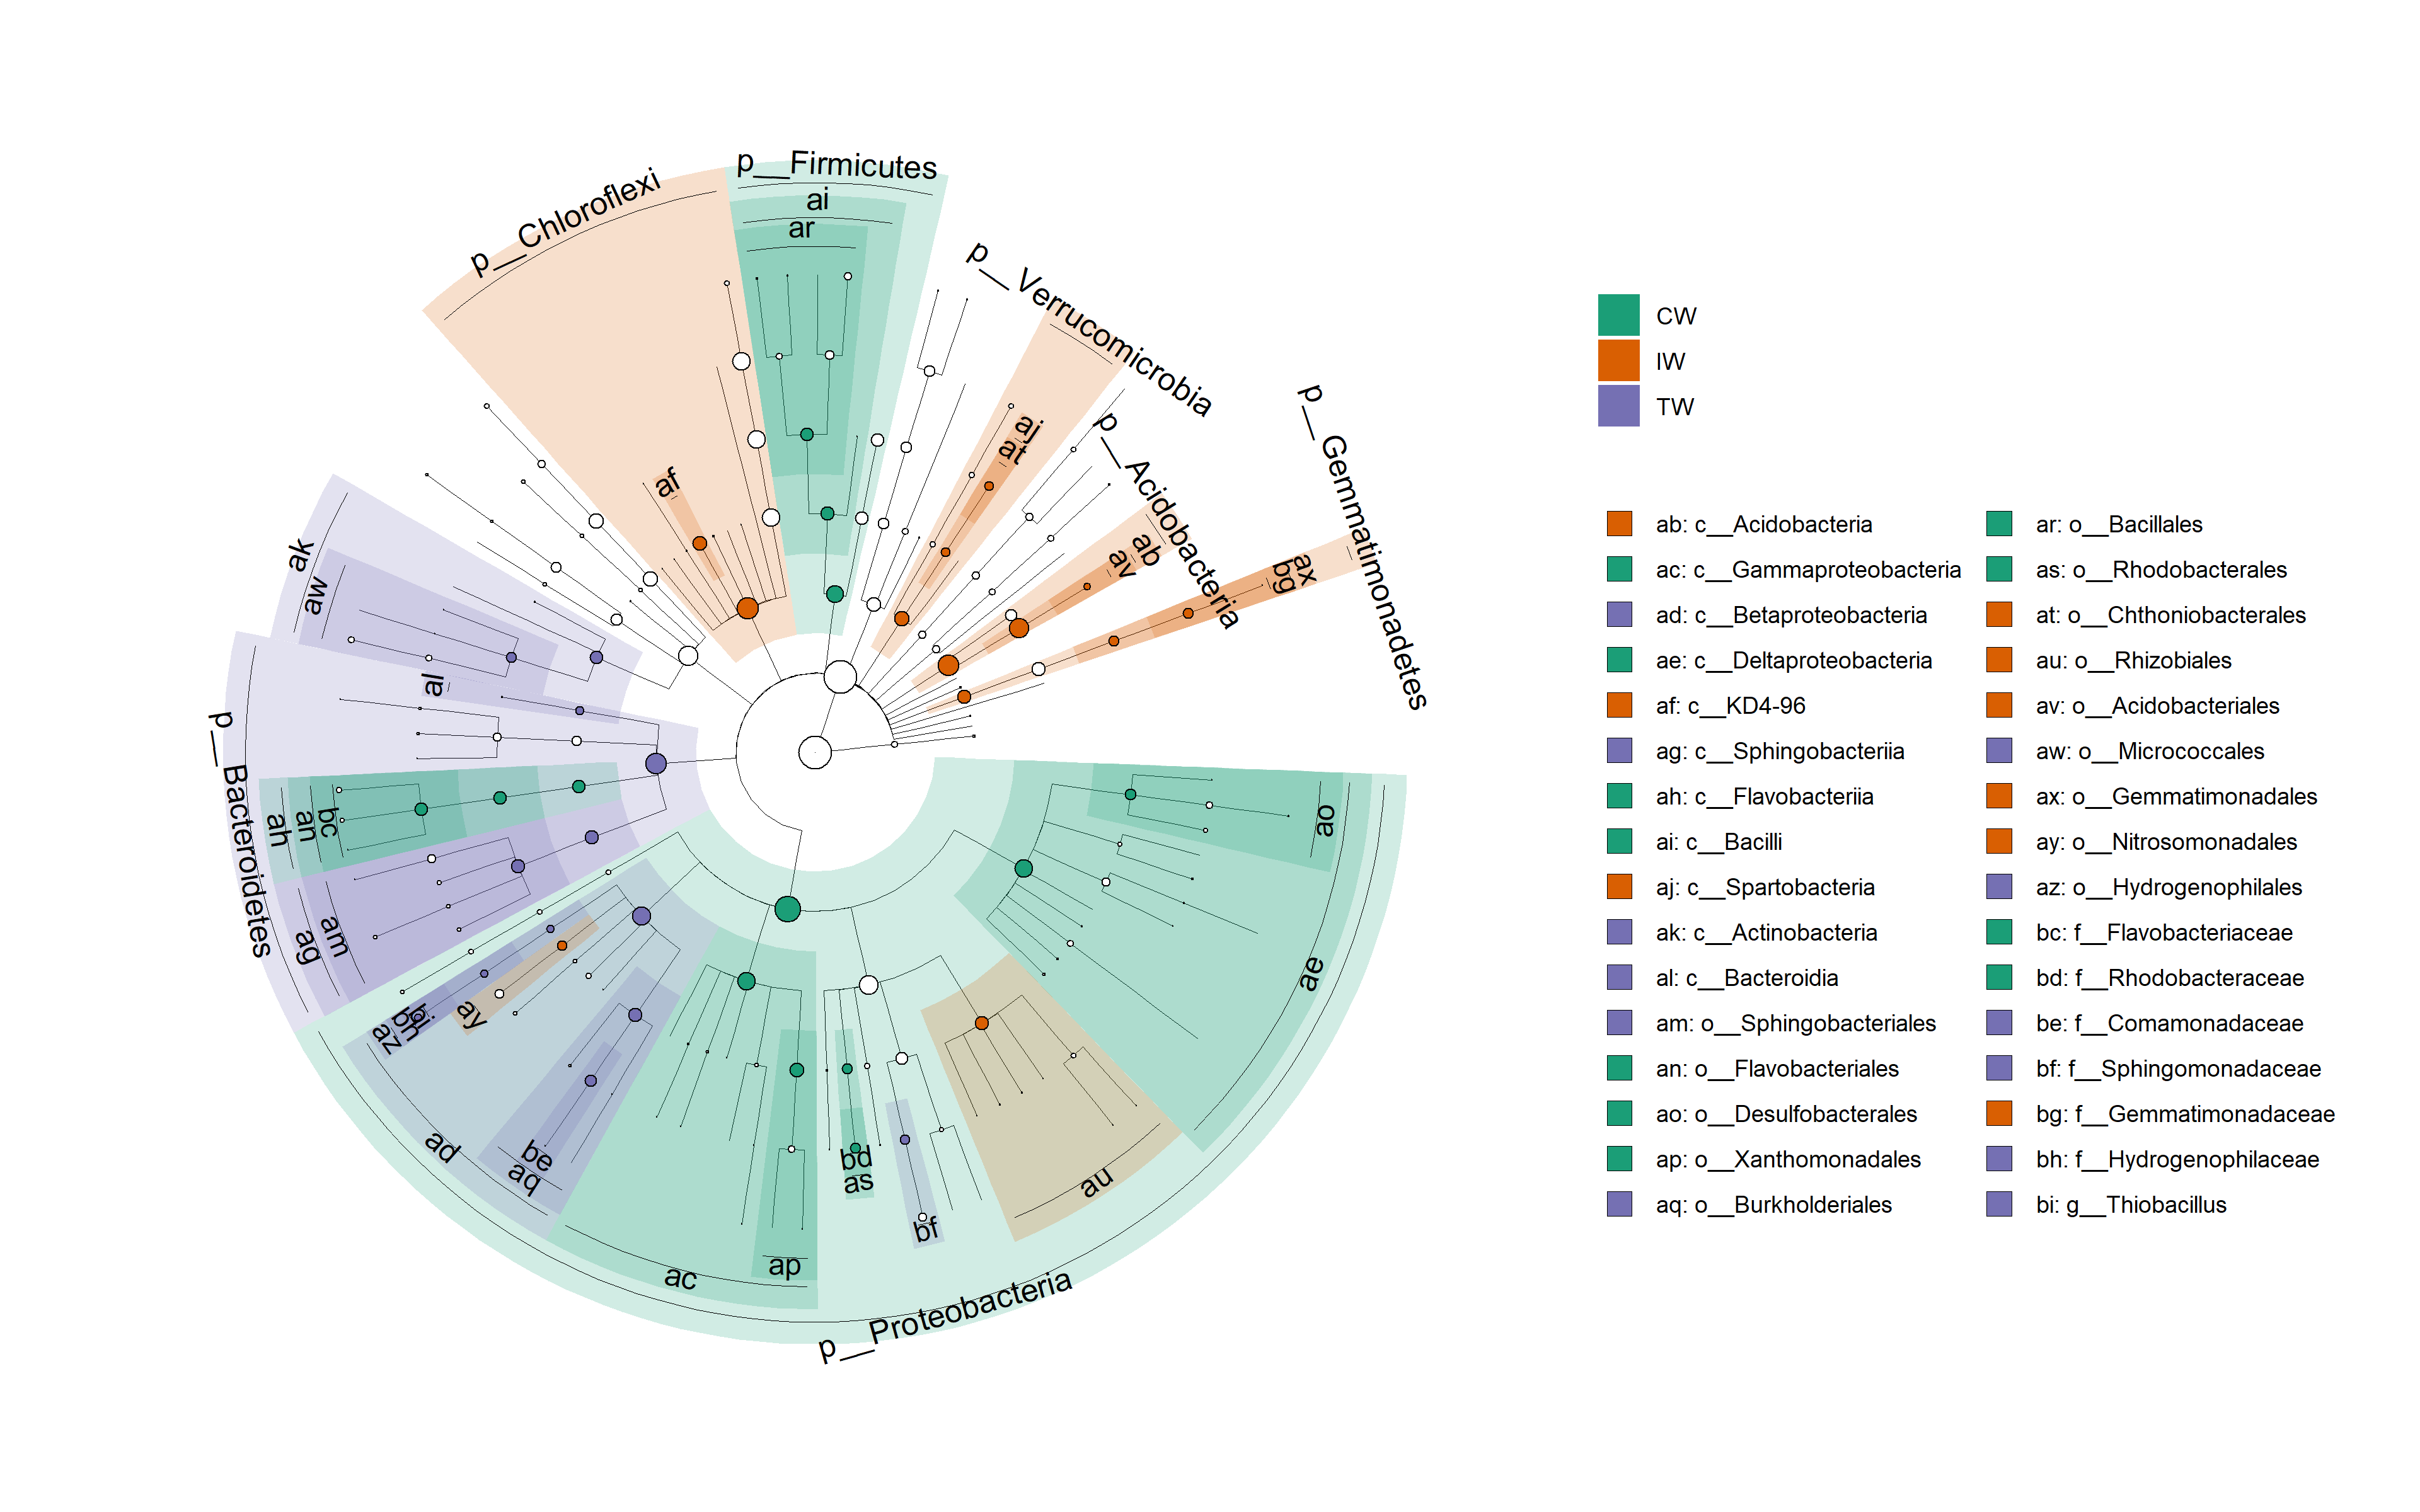
\includegraphics[width=1000px]{Images/plot_lefse_cladogram} \end{center}

There may be a problem related with the taxonomic labels in the plot.
When the levels used are too many, the taxonomic labels may have too much overlap.
However, if you only indicate the Phylum labels, the taxa in the legend with marked letters are too many.
At this time, you can select the taxa that you want to show in the plot manually like the following operation.

\begin{Shaded}
\begin{Highlighting}[]
\CommentTok{\# choose some taxa according to the positions in the previous picture; those taxa labels have minimum overlap}
\NormalTok{use\_labels }\OtherTok{\textless{}{-}} \FunctionTok{c}\NormalTok{(}\StringTok{"c\_\_Deltaproteobacteria"}\NormalTok{, }\StringTok{"c\_\_Actinobacteria"}\NormalTok{, }\StringTok{"o\_\_Rhizobiales"}\NormalTok{, }\StringTok{"p\_\_Proteobacteria"}\NormalTok{, }\StringTok{"p\_\_Bacteroidetes"}\NormalTok{, }
    \StringTok{"o\_\_Micrococcales"}\NormalTok{, }\StringTok{"p\_\_Acidobacteria"}\NormalTok{, }\StringTok{"p\_\_Verrucomicrobia"}\NormalTok{, }\StringTok{"p\_\_Firmicutes"}\NormalTok{, }
    \StringTok{"p\_\_Chloroflexi"}\NormalTok{, }\StringTok{"c\_\_Acidobacteria"}\NormalTok{, }\StringTok{"c\_\_Gammaproteobacteria"}\NormalTok{, }\StringTok{"c\_\_Betaproteobacteria"}\NormalTok{, }\StringTok{"c\_\_KD4{-}96"}\NormalTok{,}
    \StringTok{"c\_\_Bacilli"}\NormalTok{, }\StringTok{"o\_\_Gemmatimonadales"}\NormalTok{, }\StringTok{"f\_\_Gemmatimonadaceae"}\NormalTok{, }\StringTok{"o\_\_Bacillales"}\NormalTok{, }\StringTok{"o\_\_Rhodobacterales"}\NormalTok{)}
\CommentTok{\# then use parameter select\_show\_labels to show}
\NormalTok{t1}\SpecialCharTok{$}\FunctionTok{plot\_lefse\_cladogram}\NormalTok{(}\AttributeTok{use\_taxa\_num =} \DecValTok{200}\NormalTok{, }\AttributeTok{use\_feature\_num =} \DecValTok{50}\NormalTok{, }\AttributeTok{select\_show\_labels =}\NormalTok{ use\_labels)}
\CommentTok{\# Now we can see that more taxa names appear in the tree}
\end{Highlighting}
\end{Shaded}

\begin{center}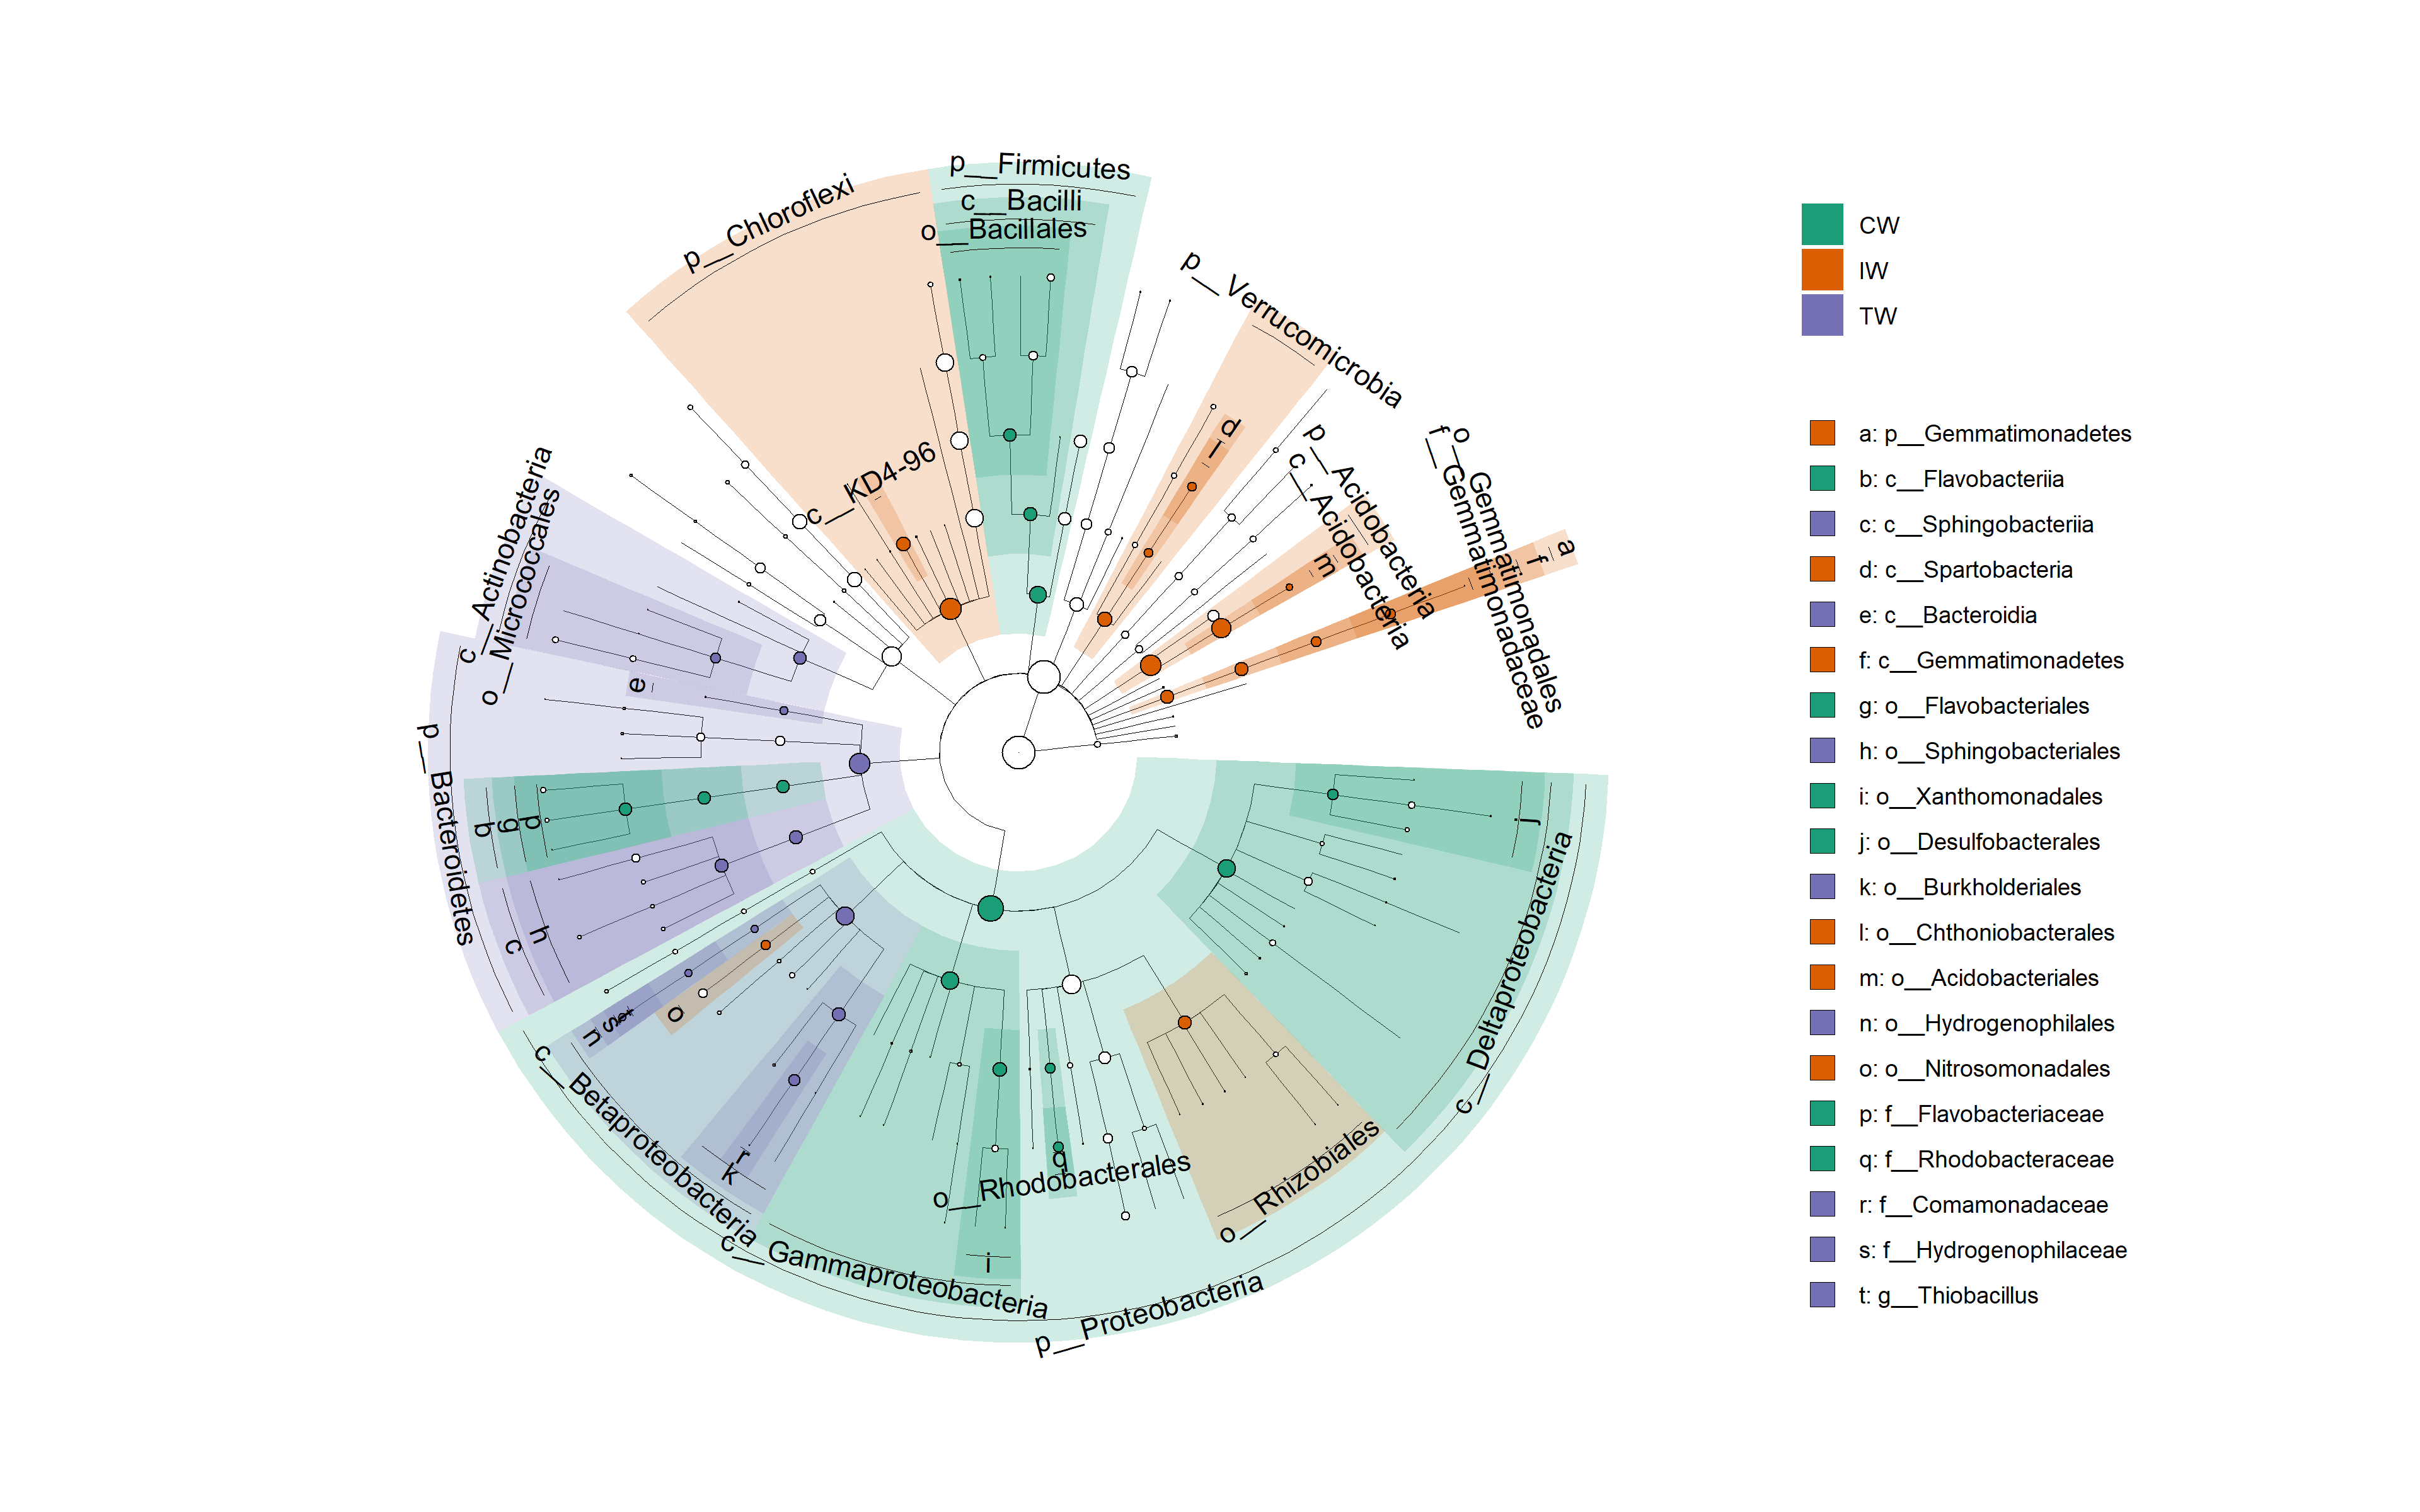
\includegraphics[width=1000px]{Images/plot_lefse_cladogram_1} \end{center}

If you are interested in taxonomic tree, you can also use metacoder package\citep{Foster_Metacoder_2017} to plot the taxonomic tree based on the selected taxa.
We do not show the usage here.

The third approach is rf, which depends on the random forest\citep{Beck_Machine_2014, Yatsunenko_Human_2012} and the non-parametric test.
The current method can calculate random forest by bootstrapping like the method in LEfSe and only use the significant features.
MeanDecreaseGini is selected as the indicator value in the analysis.

\begin{Shaded}
\begin{Highlighting}[]
\CommentTok{\# use Genus level for parameter rf\_taxa\_level, if you want to use all taxa, change to "all"}
\CommentTok{\# nresam = 1 and boots = 1 represent no bootstrapping and use all samples directly}
\NormalTok{t1 }\OtherTok{\textless{}{-}}\NormalTok{ trans\_diff}\SpecialCharTok{$}\FunctionTok{new}\NormalTok{(}\AttributeTok{dataset =}\NormalTok{ dataset, }\AttributeTok{method =} \StringTok{"rf"}\NormalTok{, }\AttributeTok{group =} \StringTok{"Group"}\NormalTok{, }\AttributeTok{rf\_taxa\_level =} \StringTok{"Genus"}\NormalTok{)}
\CommentTok{\# t1$res\_rf is the result stored in the object}
\CommentTok{\# plot the result}
\NormalTok{t2 }\OtherTok{\textless{}{-}}\NormalTok{ t1}\SpecialCharTok{$}\FunctionTok{plot\_diff\_abund}\NormalTok{(}\AttributeTok{use\_number =} \DecValTok{1}\SpecialCharTok{:}\DecValTok{20}\NormalTok{, }\AttributeTok{only\_abund\_plot =} \ConstantTok{FALSE}\NormalTok{)}
\NormalTok{gridExtra}\SpecialCharTok{::}\FunctionTok{grid.arrange}\NormalTok{(t2}\SpecialCharTok{$}\NormalTok{p1, t2}\SpecialCharTok{$}\NormalTok{p2, }\AttributeTok{ncol=}\DecValTok{2}\NormalTok{, }\AttributeTok{nrow =} \DecValTok{1}\NormalTok{, }\AttributeTok{widths =} \FunctionTok{c}\NormalTok{(}\DecValTok{2}\NormalTok{,}\DecValTok{2}\NormalTok{))}
\CommentTok{\# the middle asterisk represent the significances}
\end{Highlighting}
\end{Shaded}

\begin{center}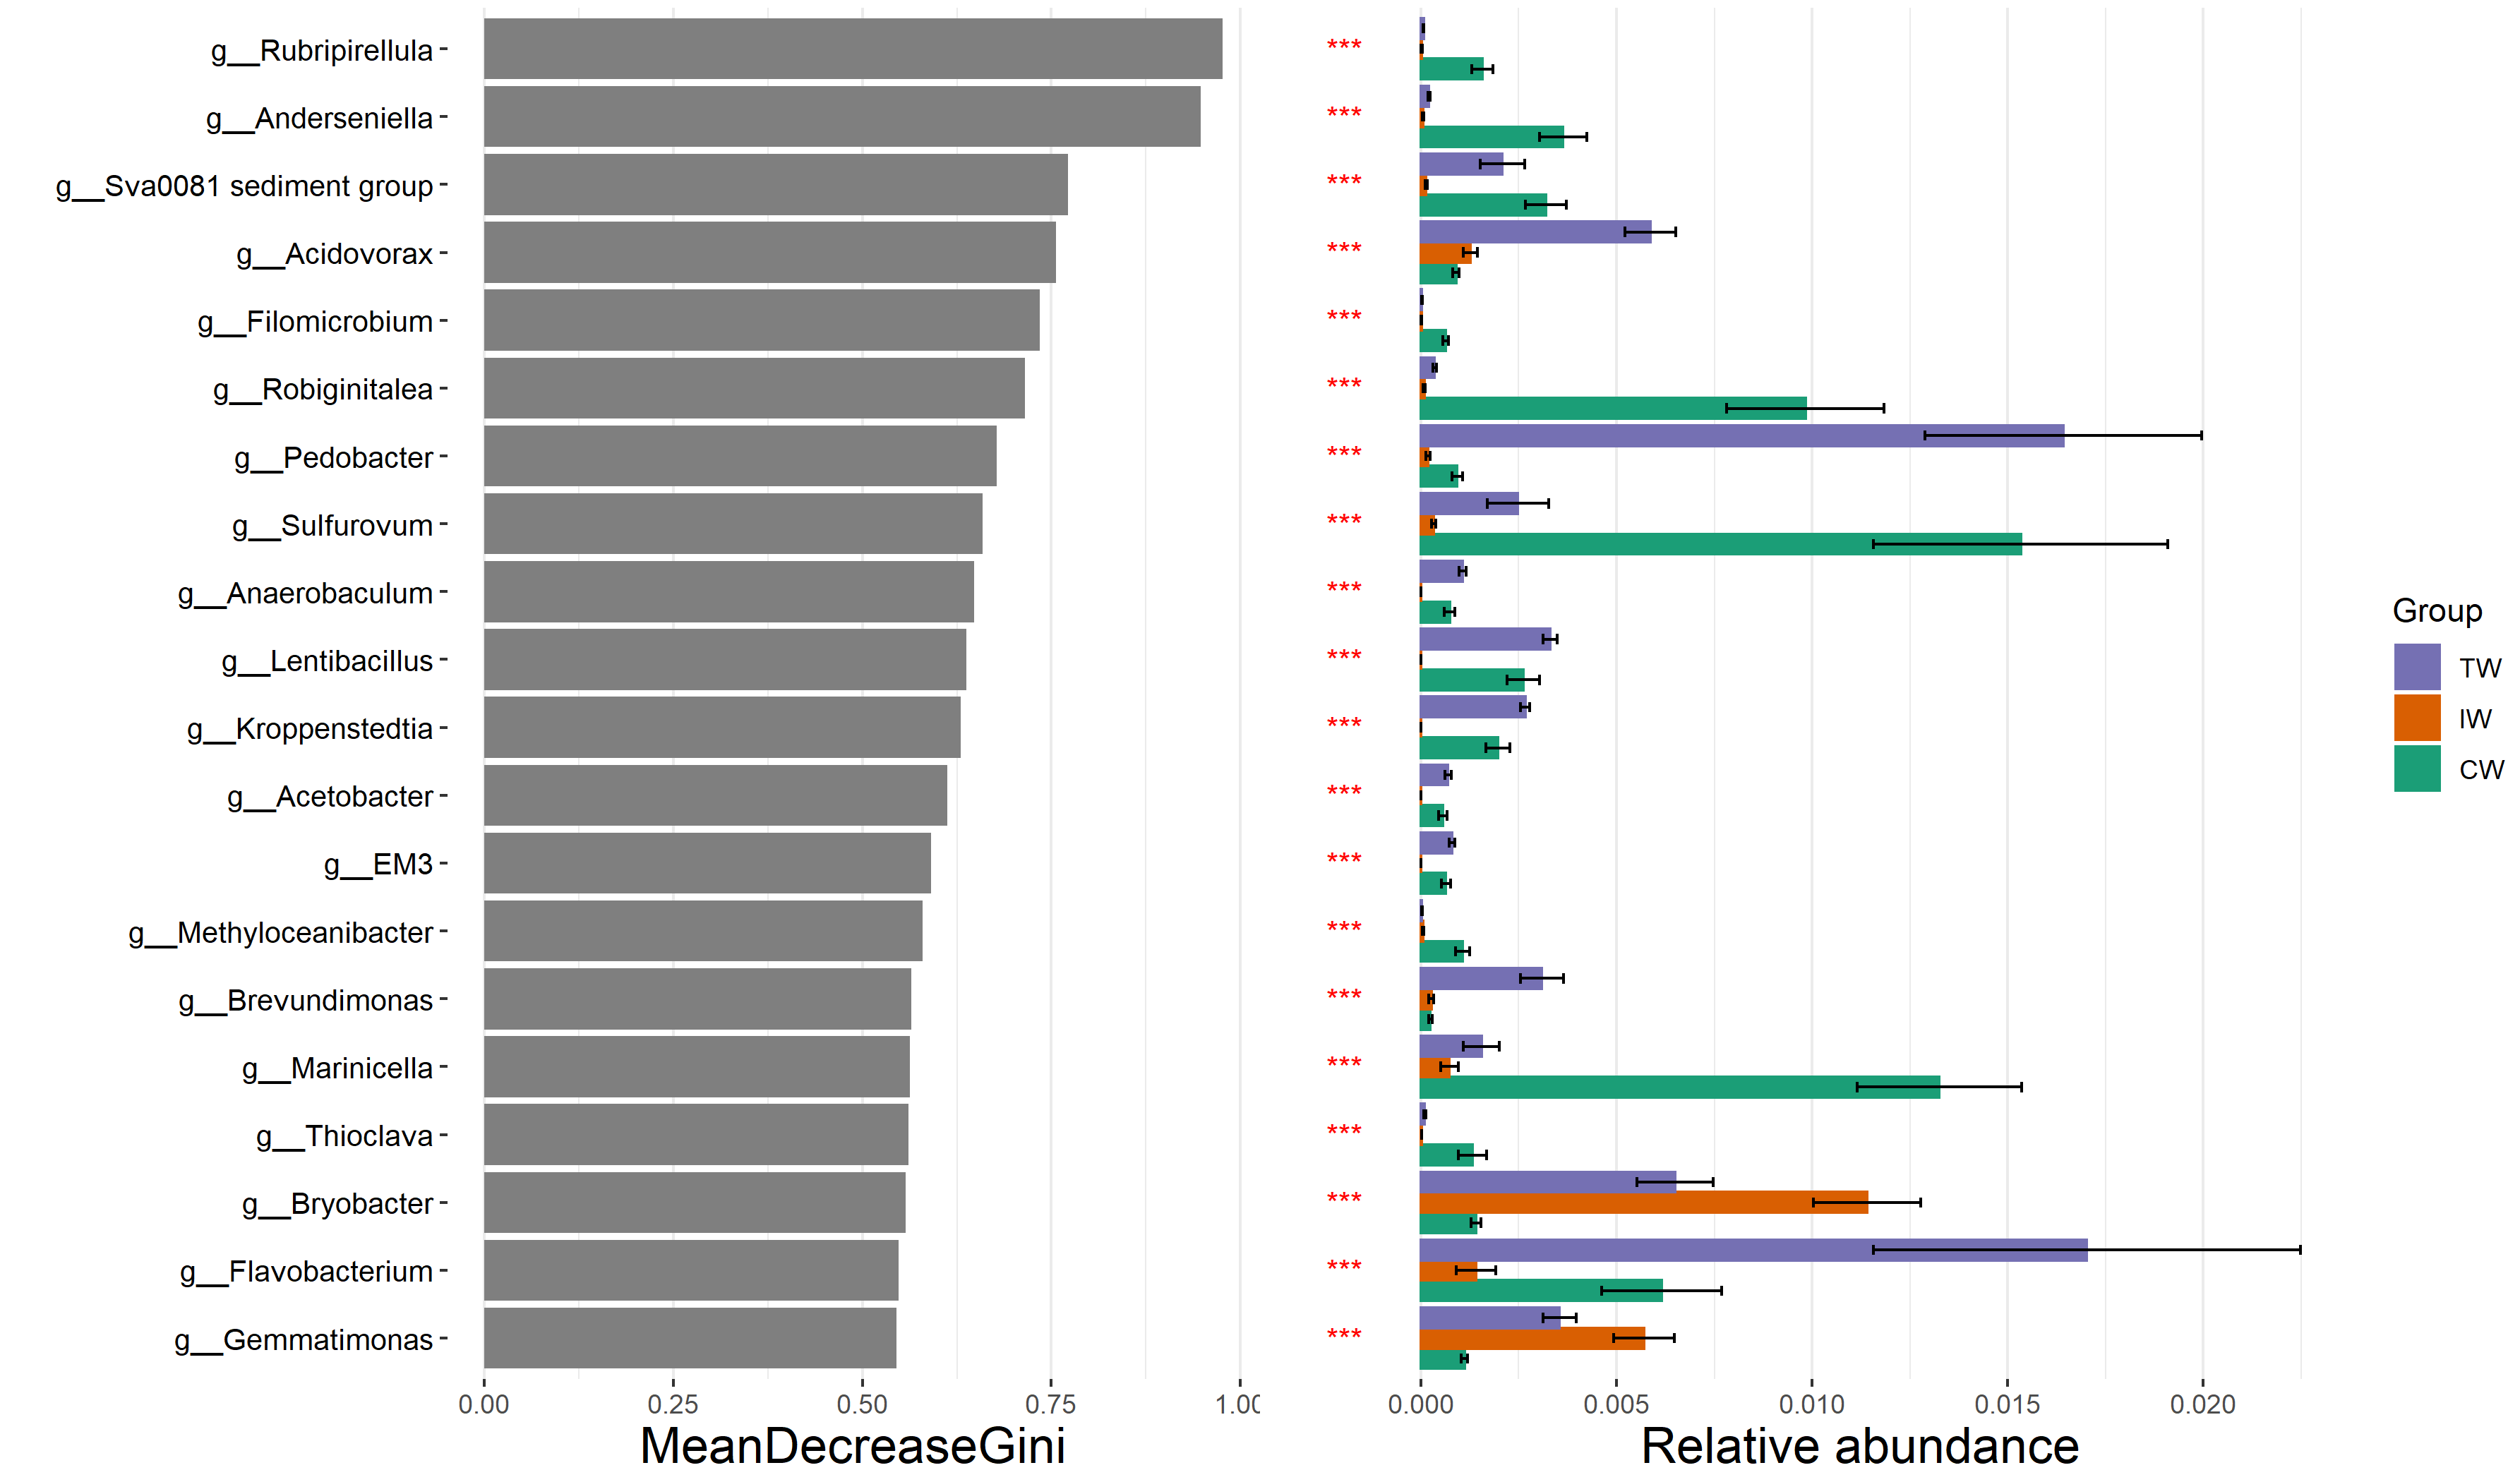
\includegraphics[width=800px]{Images/plot_diff_abund} \end{center}

\hypertarget{trans_env-class}{%
\section{trans\_env class}\label{trans_env-class}}

 The environmental variables are very useful in analyzing microbial community structure and assembly mechanisms.
We first show the RDA analysis (db-RDA and RDA).

\begin{Shaded}
\begin{Highlighting}[]
\CommentTok{\# add\_data is used to add the environmental data}
\NormalTok{t1 }\OtherTok{\textless{}{-}}\NormalTok{ trans\_env}\SpecialCharTok{$}\FunctionTok{new}\NormalTok{(}\AttributeTok{dataset =}\NormalTok{ dataset, }\AttributeTok{add\_data =}\NormalTok{ env\_data\_16S[, }\DecValTok{4}\SpecialCharTok{:}\DecValTok{11}\NormalTok{])}
\end{Highlighting}
\end{Shaded}

\begin{Shaded}
\begin{Highlighting}[]
\CommentTok{\# use bray{-}curtis distance to do dbrda}
\NormalTok{t1}\SpecialCharTok{$}\FunctionTok{cal\_rda}\NormalTok{(}\AttributeTok{use\_dbrda =} \ConstantTok{TRUE}\NormalTok{, }\AttributeTok{use\_measure =} \StringTok{"bray"}\NormalTok{)}
\CommentTok{\# t1$res\_rda is the result list stored in the object}
\NormalTok{t1}\SpecialCharTok{$}\FunctionTok{trans\_rda}\NormalTok{(}\AttributeTok{adjust\_arrow\_length =} \ConstantTok{TRUE}\NormalTok{, }\AttributeTok{max\_perc\_env =} \DecValTok{10}\NormalTok{)}
\CommentTok{\# t1$res\_rda\_trans is the transformed result for plotting}
\NormalTok{t1}\SpecialCharTok{$}\FunctionTok{plot\_rda}\NormalTok{(}\AttributeTok{plot\_color =} \StringTok{"Group"}\NormalTok{)}
\end{Highlighting}
\end{Shaded}

\begin{center}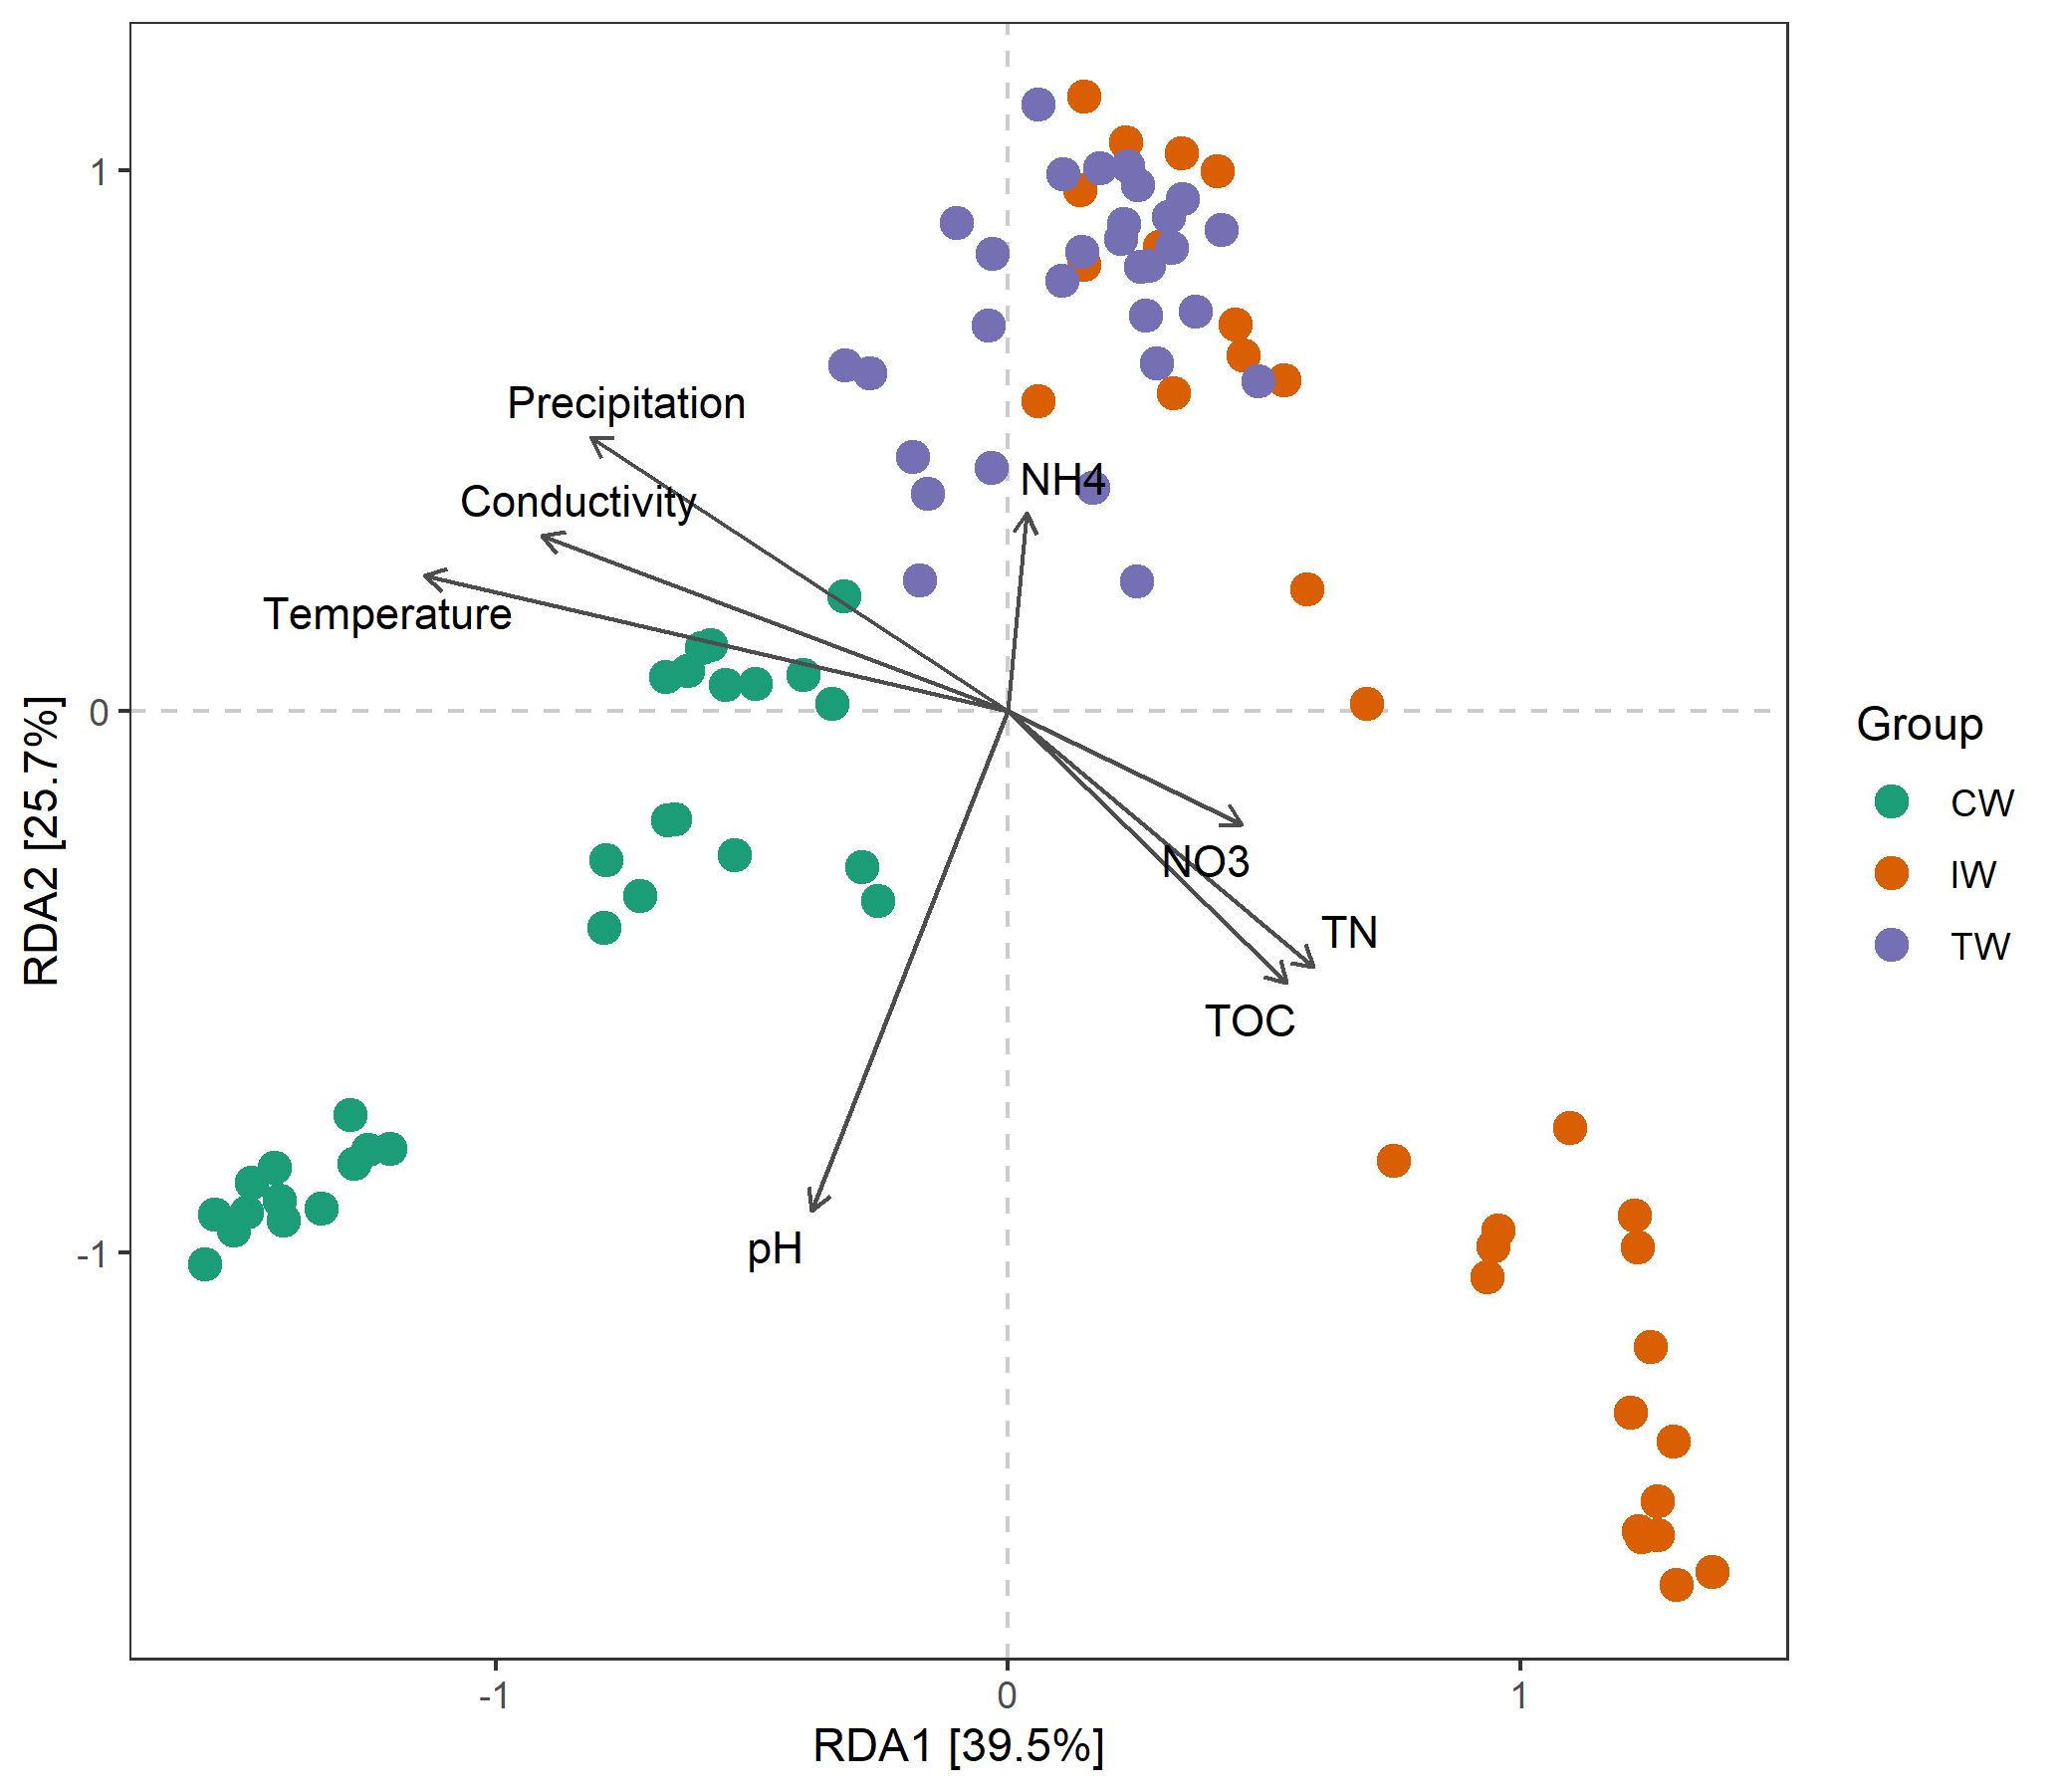
\includegraphics[width=650px]{Images/plot_rda_dbrda} \end{center}

\begin{Shaded}
\begin{Highlighting}[]
\CommentTok{\# use Genus}
\NormalTok{t1}\SpecialCharTok{$}\FunctionTok{cal\_rda}\NormalTok{(}\AttributeTok{use\_dbrda =} \ConstantTok{FALSE}\NormalTok{, }\AttributeTok{taxa\_level =} \StringTok{"Genus"}\NormalTok{)}
\CommentTok{\# As the main results of RDA are related with the projection and angles between different arrows,}
\CommentTok{\# we adjust the length of the arrow to show them clearly using several parameters.}
\NormalTok{t1}\SpecialCharTok{$}\FunctionTok{trans\_rda}\NormalTok{(}\AttributeTok{show\_taxa =} \DecValTok{10}\NormalTok{, }\AttributeTok{adjust\_arrow\_length =} \ConstantTok{TRUE}\NormalTok{, }\AttributeTok{max\_perc\_env =} \DecValTok{1500}\NormalTok{, }\AttributeTok{max\_perc\_tax =} \DecValTok{3000}\NormalTok{, }\AttributeTok{min\_perc\_env =} \DecValTok{200}\NormalTok{, }\AttributeTok{min\_perc\_tax =} \DecValTok{300}\NormalTok{)}
\CommentTok{\# t1$res\_rda\_trans is the transformed result for plotting}
\NormalTok{t1}\SpecialCharTok{$}\FunctionTok{plot\_rda}\NormalTok{(}\AttributeTok{plot\_color =} \StringTok{"Group"}\NormalTok{)}
\end{Highlighting}
\end{Shaded}

\begin{center}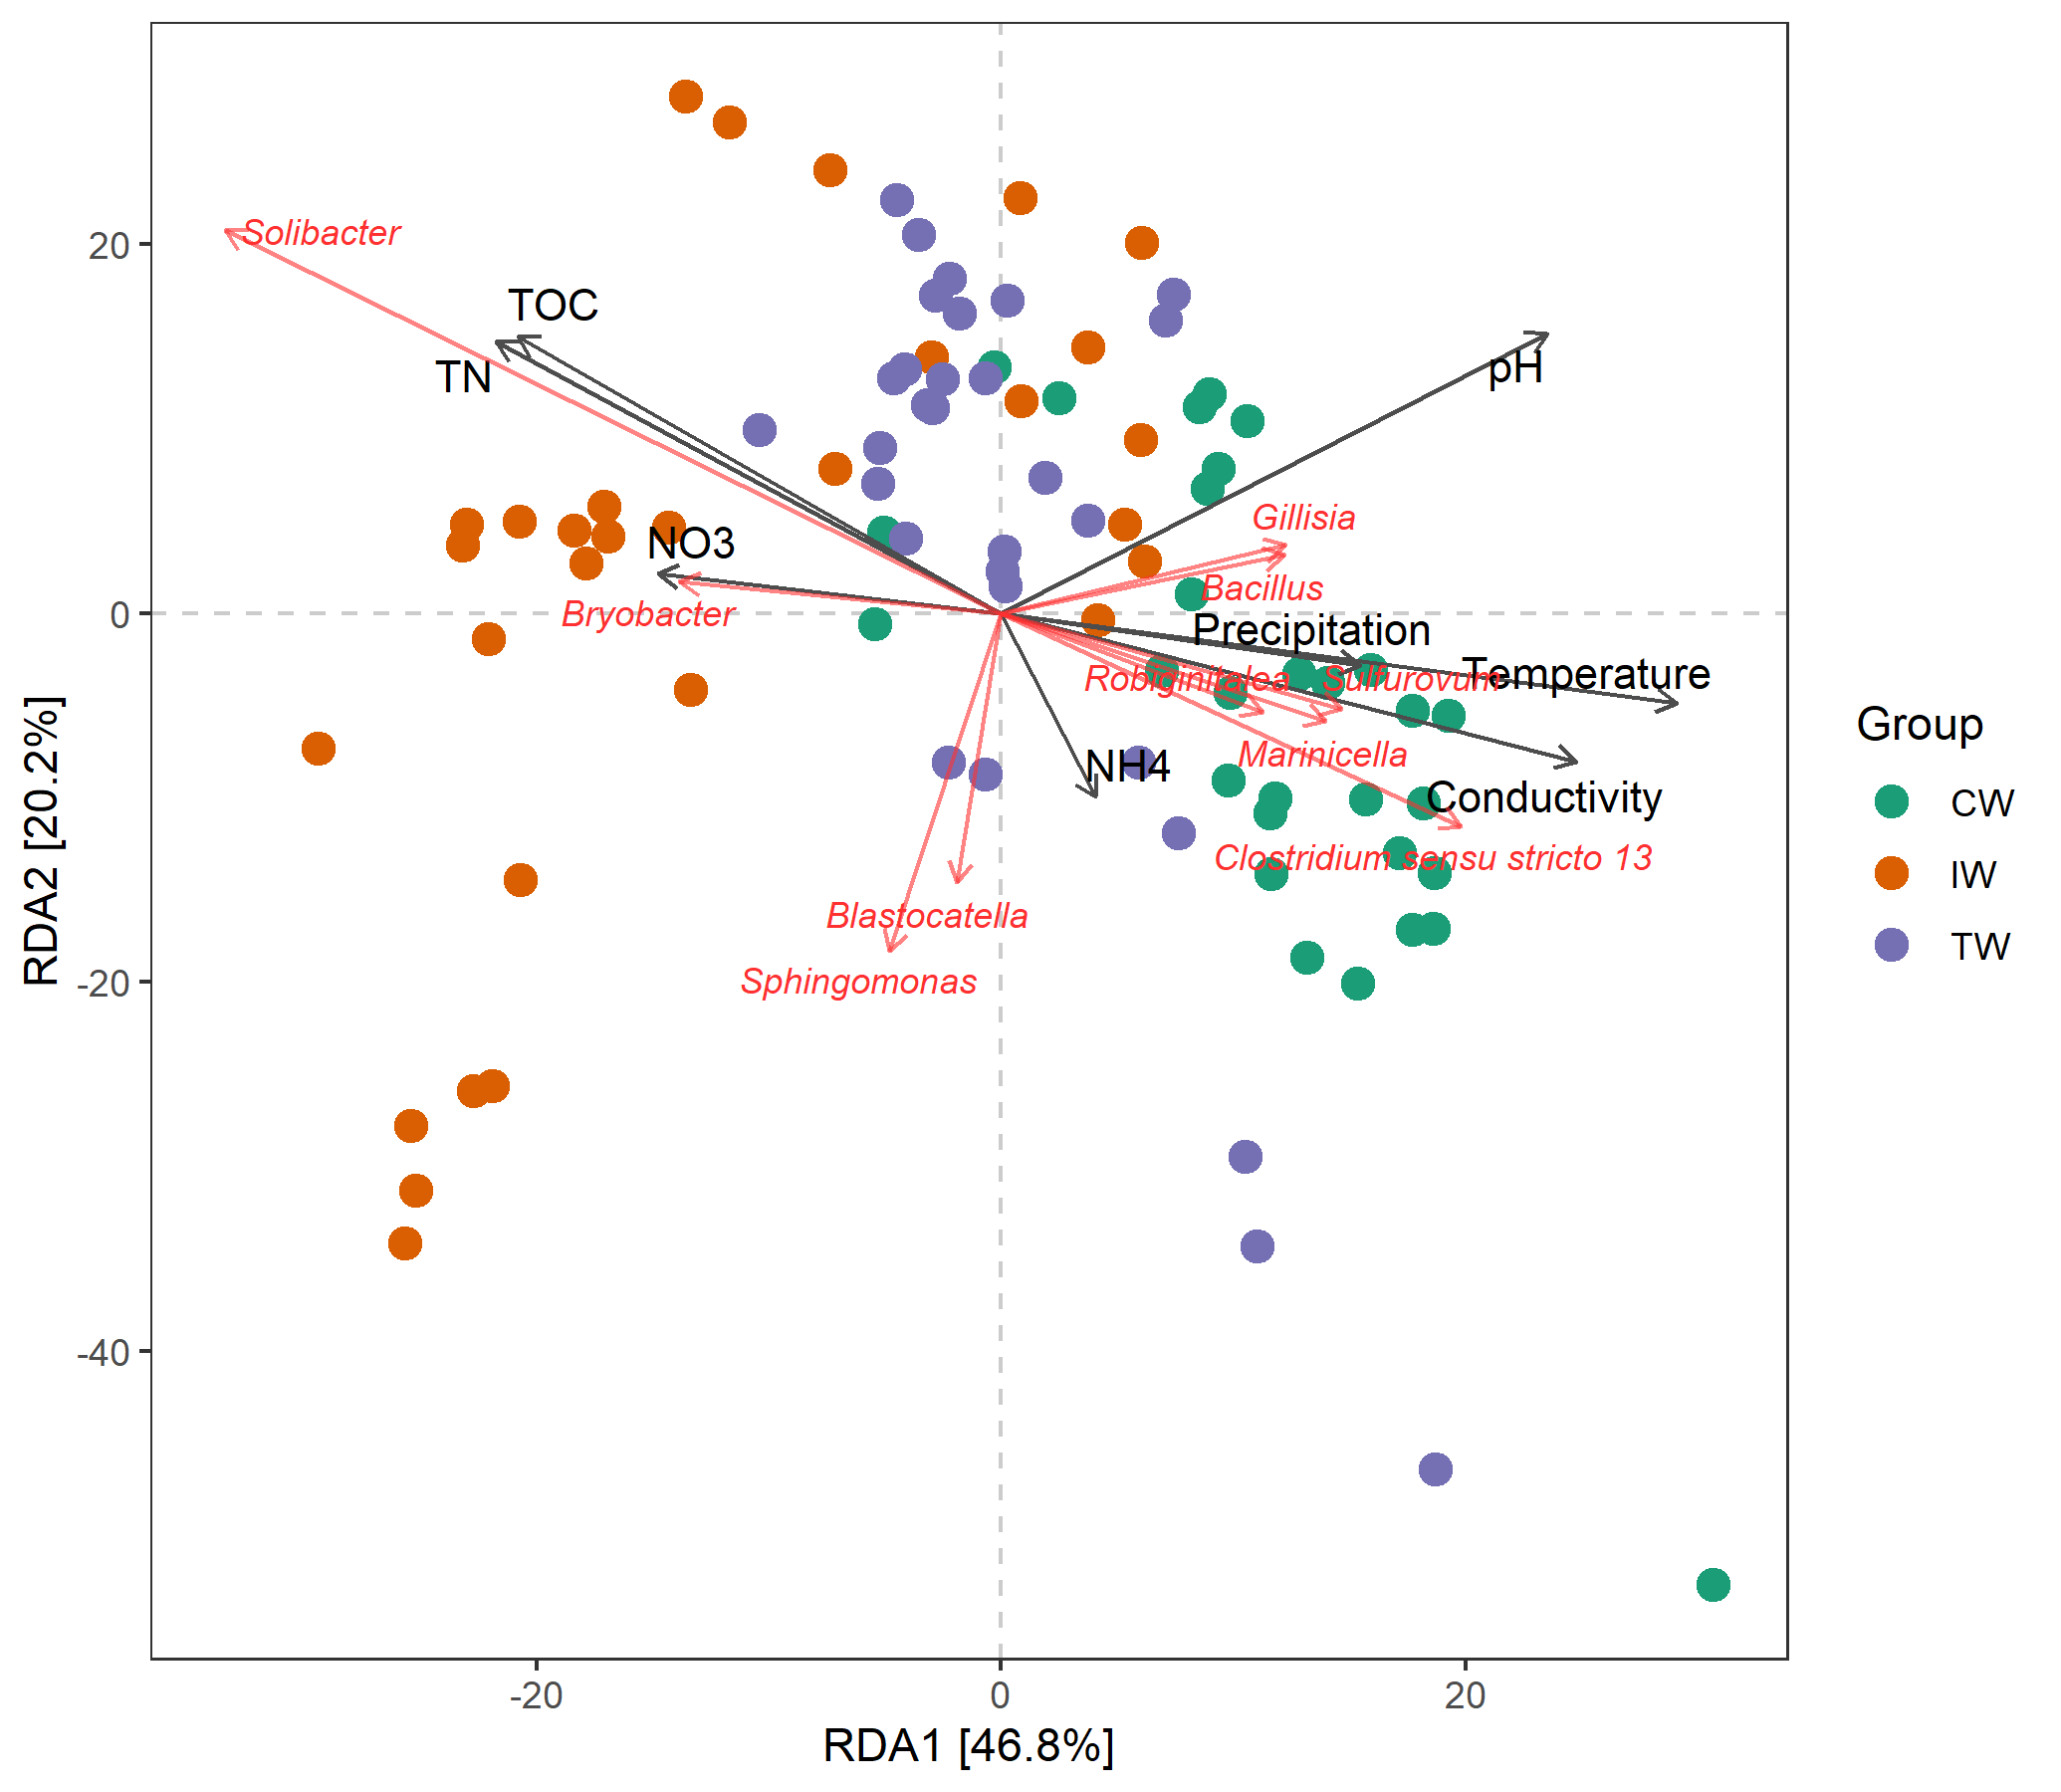
\includegraphics[width=650px]{Images/plot_rda_genus} \end{center}

Mantel test can be used to check whether there is significant correlations between environmental variables and distance matrix.

\begin{Shaded}
\begin{Highlighting}[]
\NormalTok{t1}\SpecialCharTok{$}\FunctionTok{cal\_mantel}\NormalTok{(}\AttributeTok{use\_measure =} \StringTok{"bray"}\NormalTok{)}
\CommentTok{\# return t1$res\_mantel}
\NormalTok{t1}\SpecialCharTok{$}\NormalTok{res\_mantel}
\end{Highlighting}
\end{Shaded}

\begin{verbatim}
## The result is stored in object$res_mantel or object$res_mantel_partial ...
\end{verbatim}

\begin{longtable}[]{@{}
  >{\centering\arraybackslash}p{(\columnwidth - 8\tabcolsep) * \real{0.22}}
  >{\centering\arraybackslash}p{(\columnwidth - 8\tabcolsep) * \real{0.18}}
  >{\centering\arraybackslash}p{(\columnwidth - 8\tabcolsep) * \real{0.15}}
  >{\centering\arraybackslash}p{(\columnwidth - 8\tabcolsep) * \real{0.11}}
  >{\centering\arraybackslash}p{(\columnwidth - 8\tabcolsep) * \real{0.21}}@{}}
\toprule
variable\_name & cor\_method & corr\_res & p\_res & significance \\
\midrule
\endhead
Temperature & pearson & 0.452 & 0.001 & *** \\
Precipitation & pearson & 0.2791 & 0.001 & *** \\
TOC & pearson & 0.13 & 0.003 & ** \\
NH4 & pearson & -0.05539 & 0.926 & \\
NO3 & pearson & 0.06758 & 0.05 & * \\
pH & pearson & 0.4085 & 0.001 & *** \\
Conductivity & pearson & 0.2643 & 0.001 & *** \\
TN & pearson & 0.1321 & 0.002 & ** \\
\bottomrule
\end{longtable}

The correlations between environmental variables and taxa are important in analyzing and inferring the factors affecting community structure.
In this example, we first perform the differential abundance test and random forest analysis to obtain the important genera.
Then we use those taxa to perform correlation analysis.

\begin{Shaded}
\begin{Highlighting}[]
\CommentTok{\# first create trans\_diff object}
\NormalTok{t2 }\OtherTok{\textless{}{-}}\NormalTok{ trans\_diff}\SpecialCharTok{$}\FunctionTok{new}\NormalTok{(}\AttributeTok{dataset =}\NormalTok{ dataset, }\AttributeTok{method =} \StringTok{"rf"}\NormalTok{, }\AttributeTok{group =} \StringTok{"Group"}\NormalTok{, }\AttributeTok{rf\_taxa\_level =} \StringTok{"Genus"}\NormalTok{)}
\end{Highlighting}
\end{Shaded}

\begin{verbatim}
## Start differential test for Group ...
\end{verbatim}

\begin{verbatim}
## Total 432 biomarkers found ...
\end{verbatim}

\begin{verbatim}
## The result is stored in object$res_rf ...
\end{verbatim}

\begin{verbatim}
## The abundance is stored in object$res_abund ...
\end{verbatim}

\begin{Shaded}
\begin{Highlighting}[]
\CommentTok{\# then create trans\_env object}
\NormalTok{t1 }\OtherTok{\textless{}{-}}\NormalTok{ trans\_env}\SpecialCharTok{$}\FunctionTok{new}\NormalTok{(}\AttributeTok{dataset =}\NormalTok{ dataset, }\AttributeTok{add\_data =}\NormalTok{ env\_data\_16S[, }\DecValTok{4}\SpecialCharTok{:}\DecValTok{11}\NormalTok{])}
\CommentTok{\# calculate correlation}
\NormalTok{t1}\SpecialCharTok{$}\FunctionTok{cal\_cor}\NormalTok{(}\AttributeTok{use\_data =} \StringTok{"other"}\NormalTok{, }\AttributeTok{p\_adjust\_method =} \StringTok{"fdr"}\NormalTok{, }\AttributeTok{other\_taxa =}\NormalTok{ t2}\SpecialCharTok{$}\NormalTok{res\_rf}\SpecialCharTok{$}\NormalTok{Taxa[}\DecValTok{1}\SpecialCharTok{:}\DecValTok{40}\NormalTok{])}
\end{Highlighting}
\end{Shaded}

\begin{verbatim}
## The correlation result is stored in object$res_cor ...
\end{verbatim}

\begin{Shaded}
\begin{Highlighting}[]
\CommentTok{\# return t1$res\_cor }
\end{Highlighting}
\end{Shaded}

Then, we can plot the correlation results using ggplot2 or pheatmap.

\begin{Shaded}
\begin{Highlighting}[]
\CommentTok{\# default ggplot2 method}
\NormalTok{t1}\SpecialCharTok{$}\FunctionTok{plot\_cor}\NormalTok{()}
\end{Highlighting}
\end{Shaded}

\begin{center}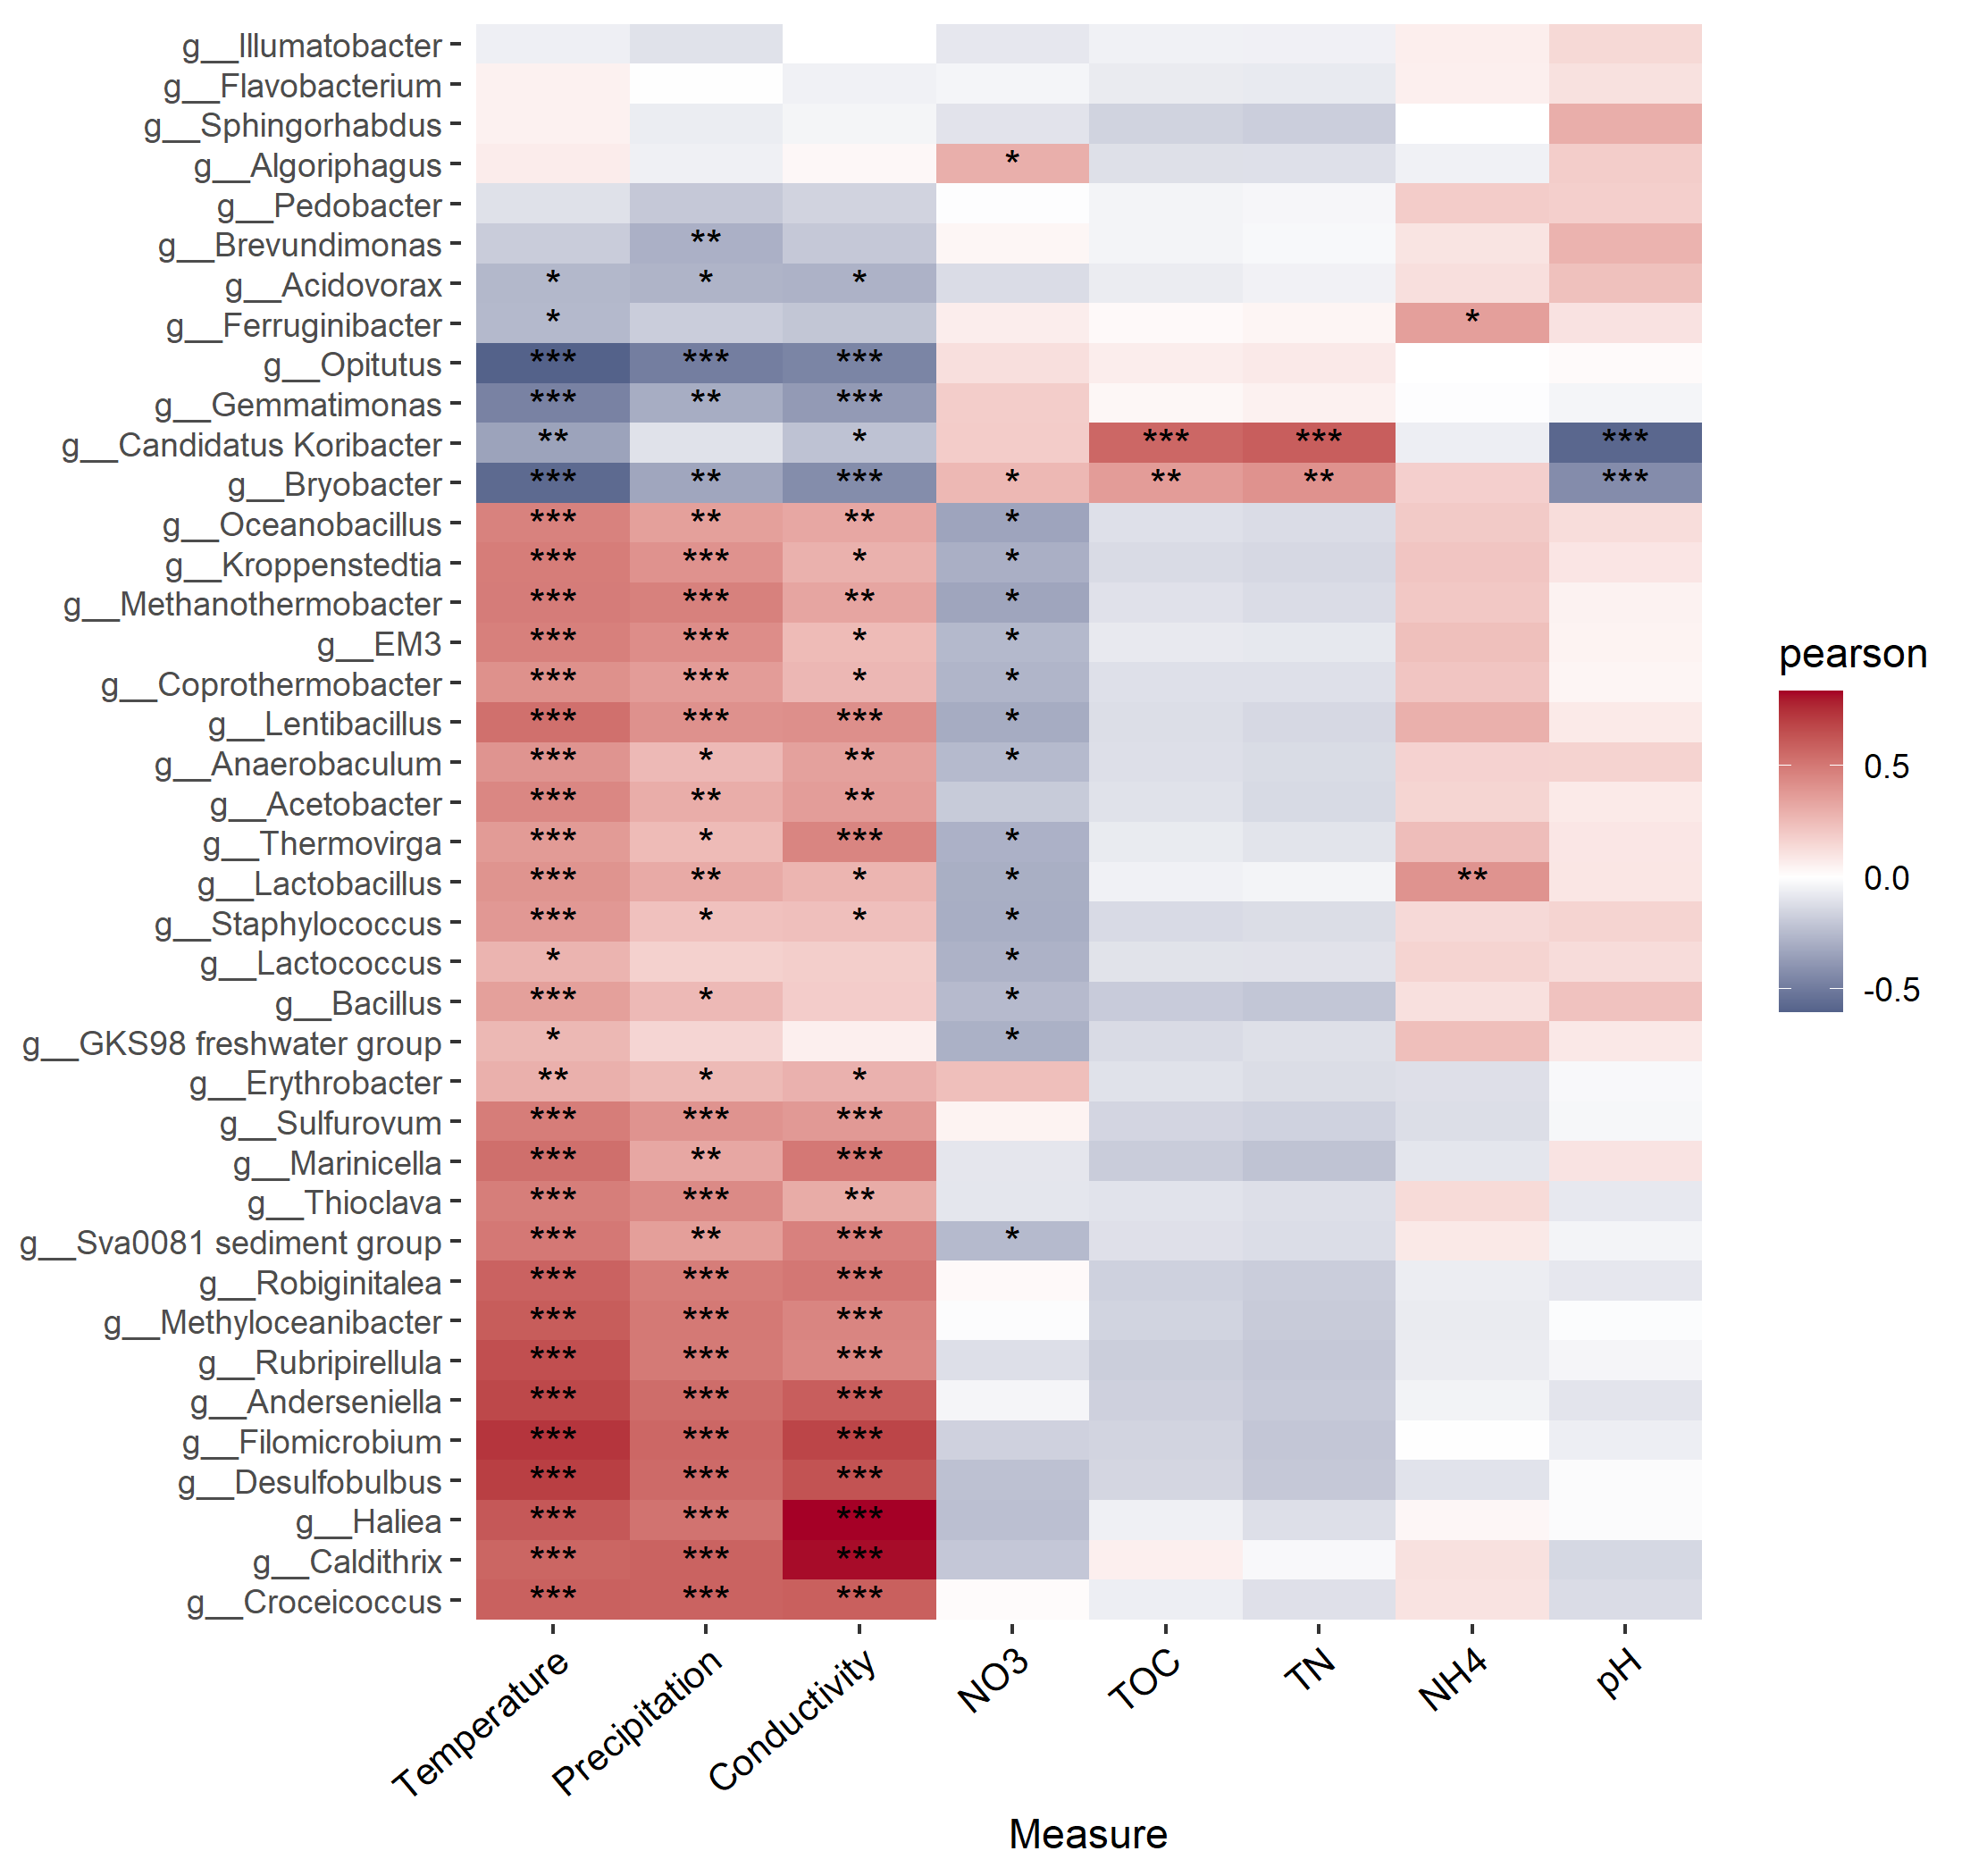
\includegraphics[width=700px]{Images/plot_corr_ggplot} \end{center}

\begin{Shaded}
\begin{Highlighting}[]
\CommentTok{\# clustering heatmap; require pheatmap package}
\NormalTok{t1}\SpecialCharTok{$}\FunctionTok{plot\_cor}\NormalTok{(}\AttributeTok{pheatmap =} \ConstantTok{TRUE}\NormalTok{)}
\end{Highlighting}
\end{Shaded}

\begin{center}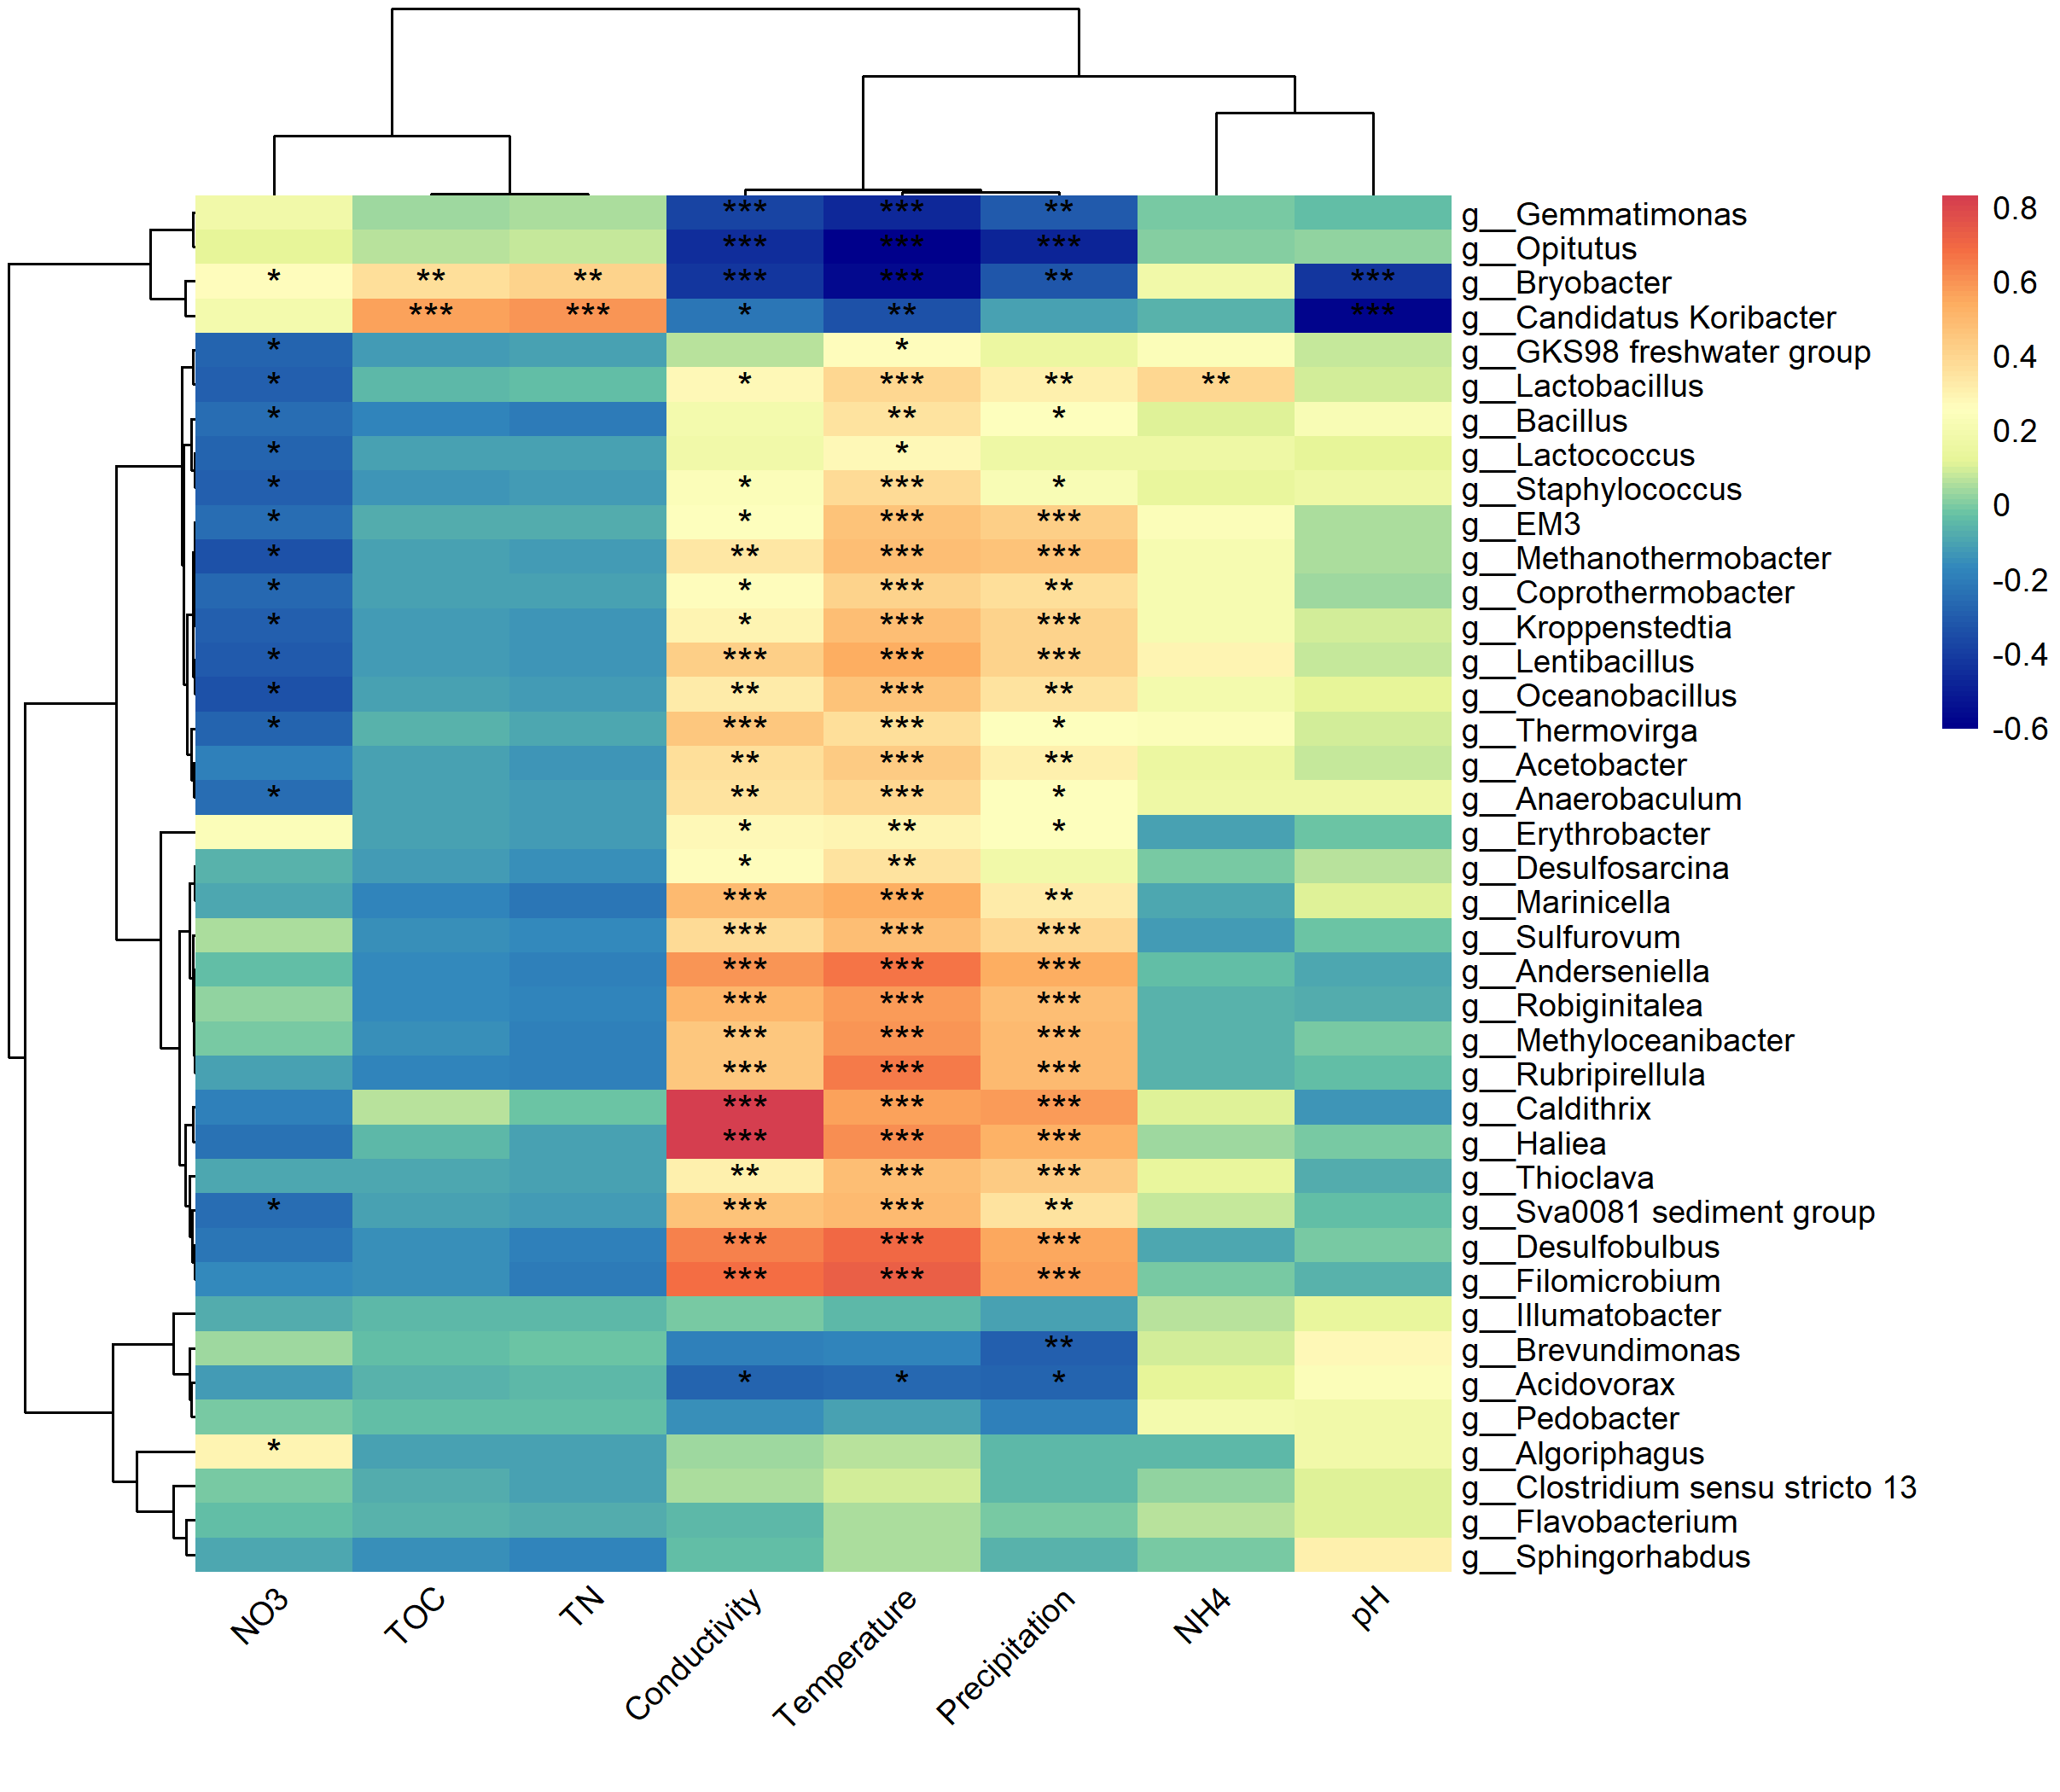
\includegraphics[width=700px]{Images/plot_corr_pheatmap} \end{center}

Sometimes, it is necessary to study the correlations between environmental variables and taxa for different groups.

\begin{Shaded}
\begin{Highlighting}[]
\CommentTok{\# calculate correlations for different groups using parameter by\_group}
\NormalTok{t1}\SpecialCharTok{$}\FunctionTok{cal\_cor}\NormalTok{(}\AttributeTok{by\_group =} \StringTok{"Group"}\NormalTok{, }\AttributeTok{use\_data =} \StringTok{"other"}\NormalTok{, }\AttributeTok{p\_adjust\_method =} \StringTok{"fdr"}\NormalTok{, }\AttributeTok{other\_taxa =}\NormalTok{ t2}\SpecialCharTok{$}\NormalTok{res\_rf}\SpecialCharTok{$}\NormalTok{Taxa[}\DecValTok{1}\SpecialCharTok{:}\DecValTok{40}\NormalTok{])}
\CommentTok{\# return t1$res\_cor}
\NormalTok{t1}\SpecialCharTok{$}\FunctionTok{plot\_cor}\NormalTok{()}
\end{Highlighting}
\end{Shaded}

\begin{center}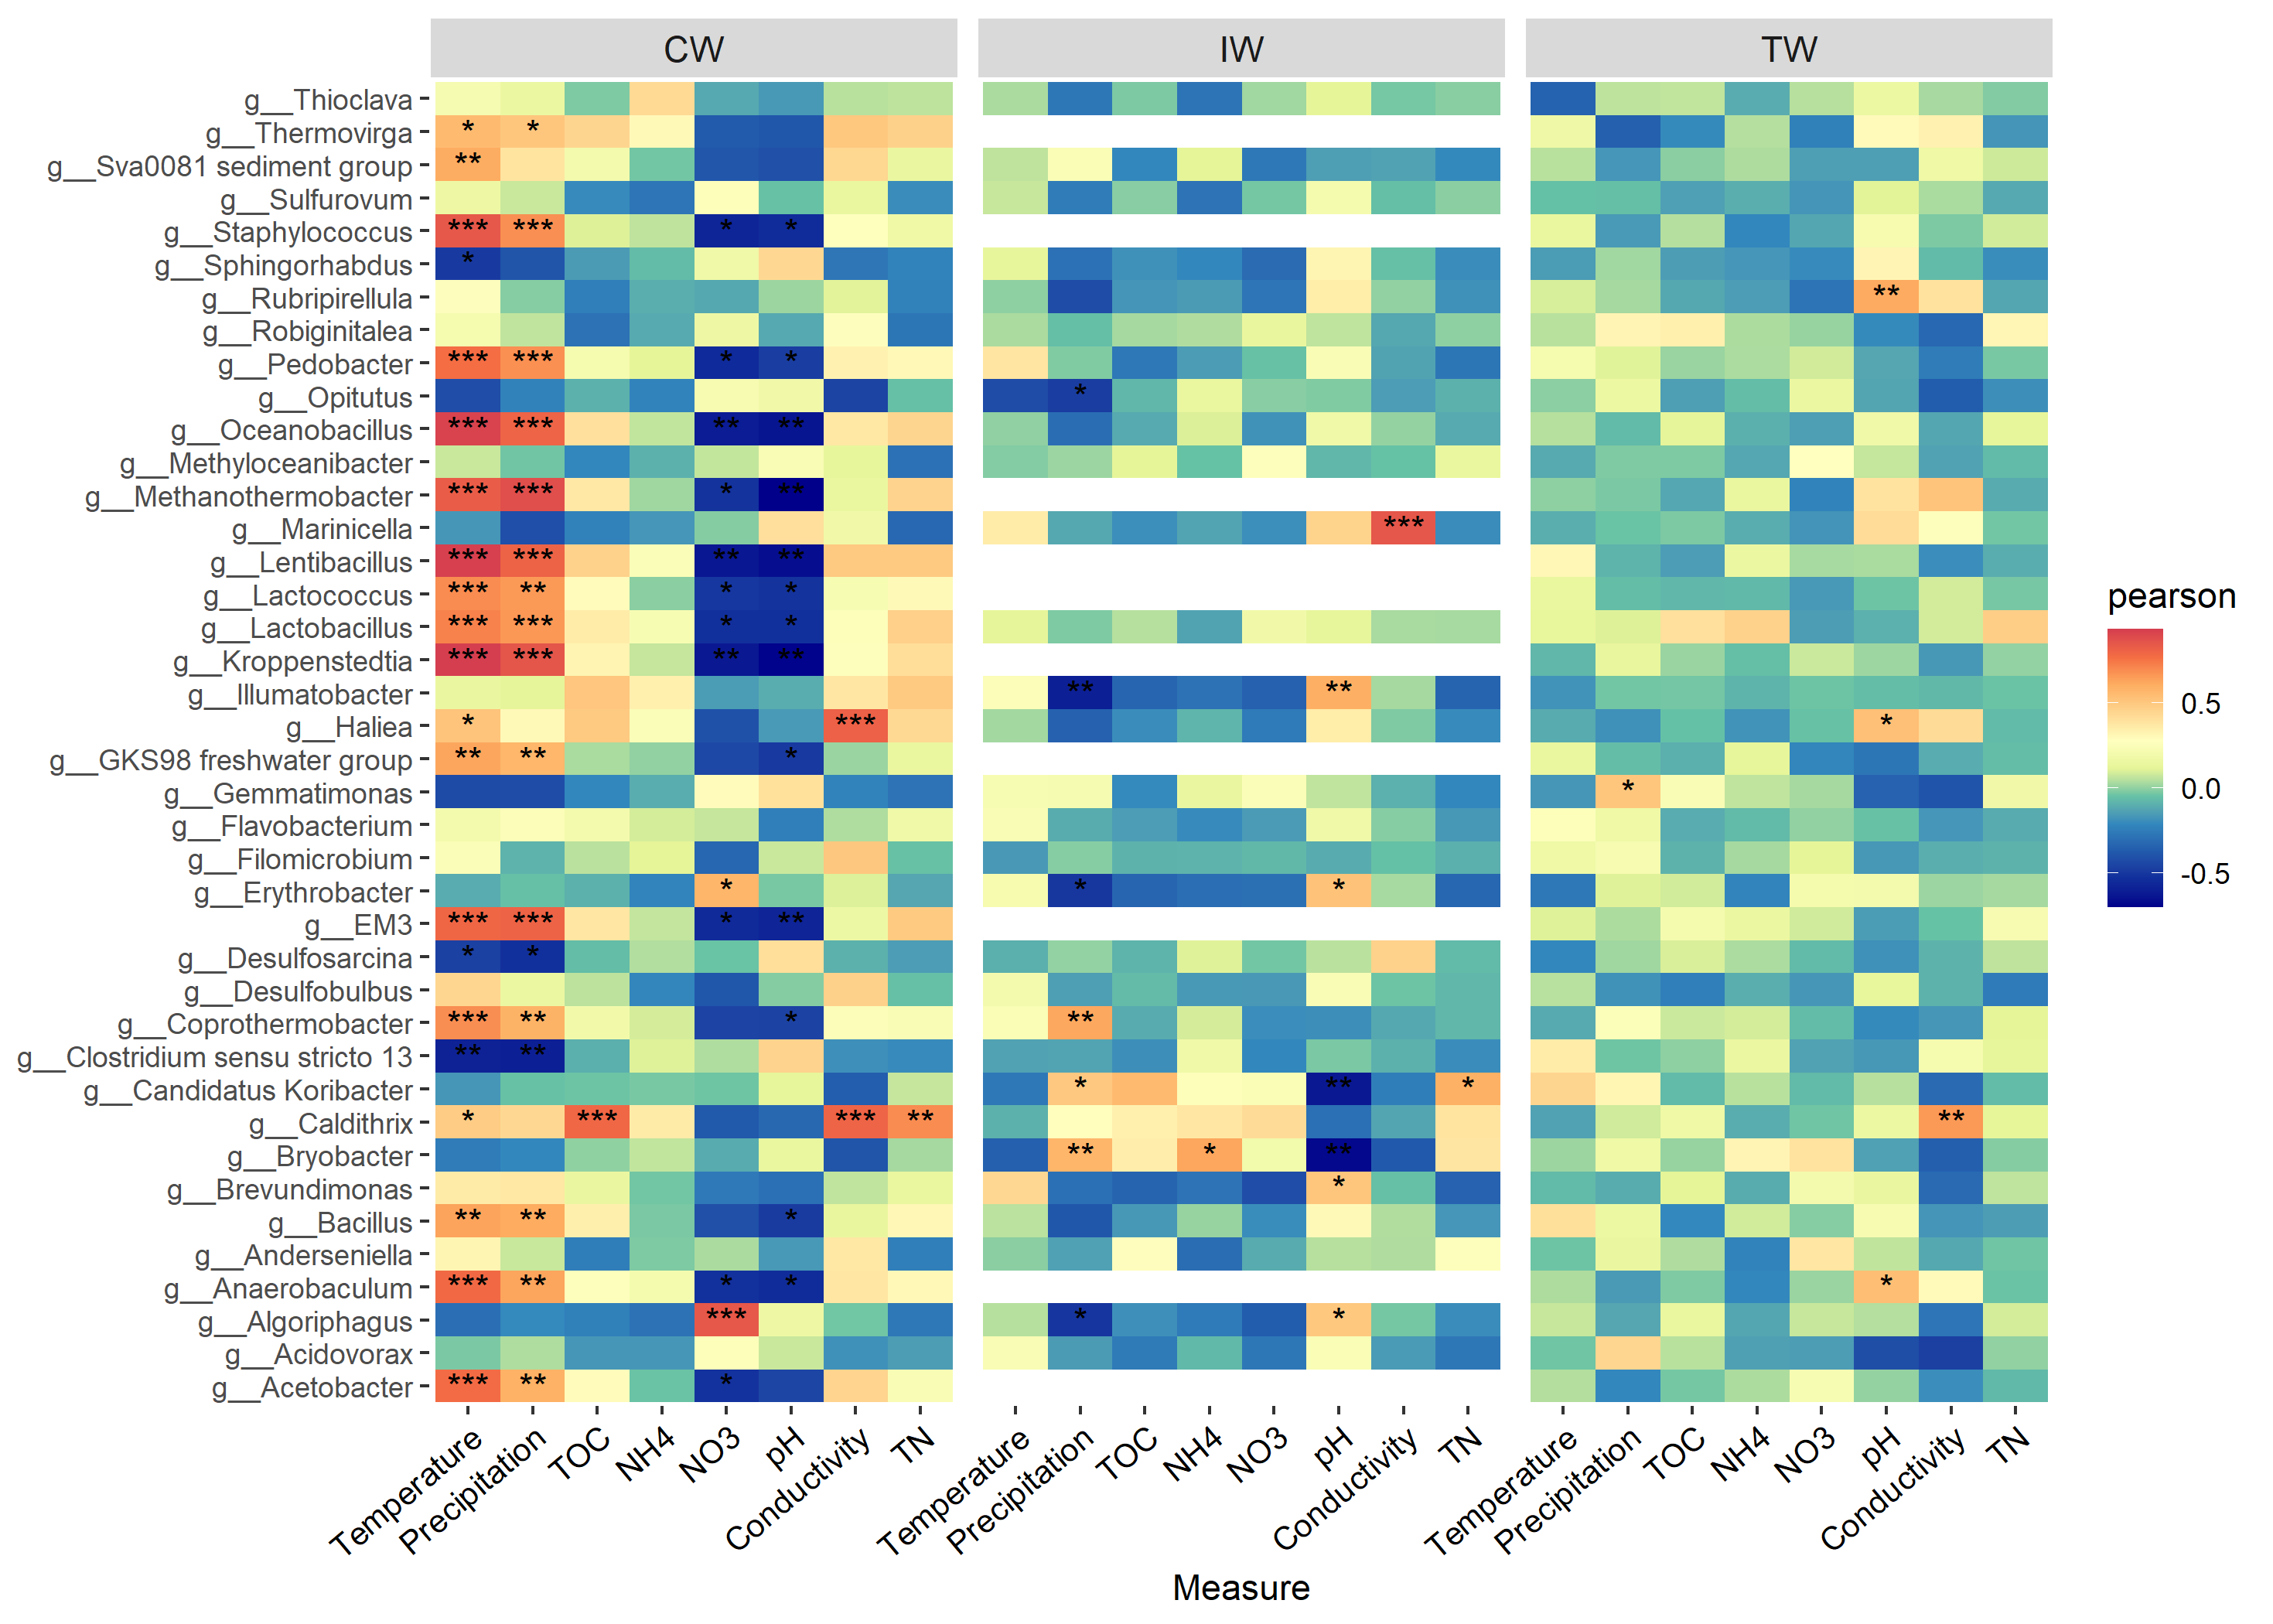
\includegraphics[width=700px]{Images/plot_corr_ggplot_groups} \end{center}

If you are concerned with the relationship between environmental factors and alpha diversity, you can also use this function.

\begin{Shaded}
\begin{Highlighting}[]
\NormalTok{t1 }\OtherTok{\textless{}{-}}\NormalTok{ trans\_env}\SpecialCharTok{$}\FunctionTok{new}\NormalTok{(}\AttributeTok{dataset =}\NormalTok{ dataset, }\AttributeTok{add\_data =}\NormalTok{ env\_data\_16S[, }\DecValTok{4}\SpecialCharTok{:}\DecValTok{11}\NormalTok{])}
\CommentTok{\# use add\_abund\_table parameter to add the extra data table}
\NormalTok{t1}\SpecialCharTok{$}\FunctionTok{cal\_cor}\NormalTok{(}\AttributeTok{add\_abund\_table =}\NormalTok{ dataset}\SpecialCharTok{$}\NormalTok{alpha\_diversity)}
\NormalTok{t1}\SpecialCharTok{$}\FunctionTok{plot\_cor}\NormalTok{()}
\end{Highlighting}
\end{Shaded}

\begin{center}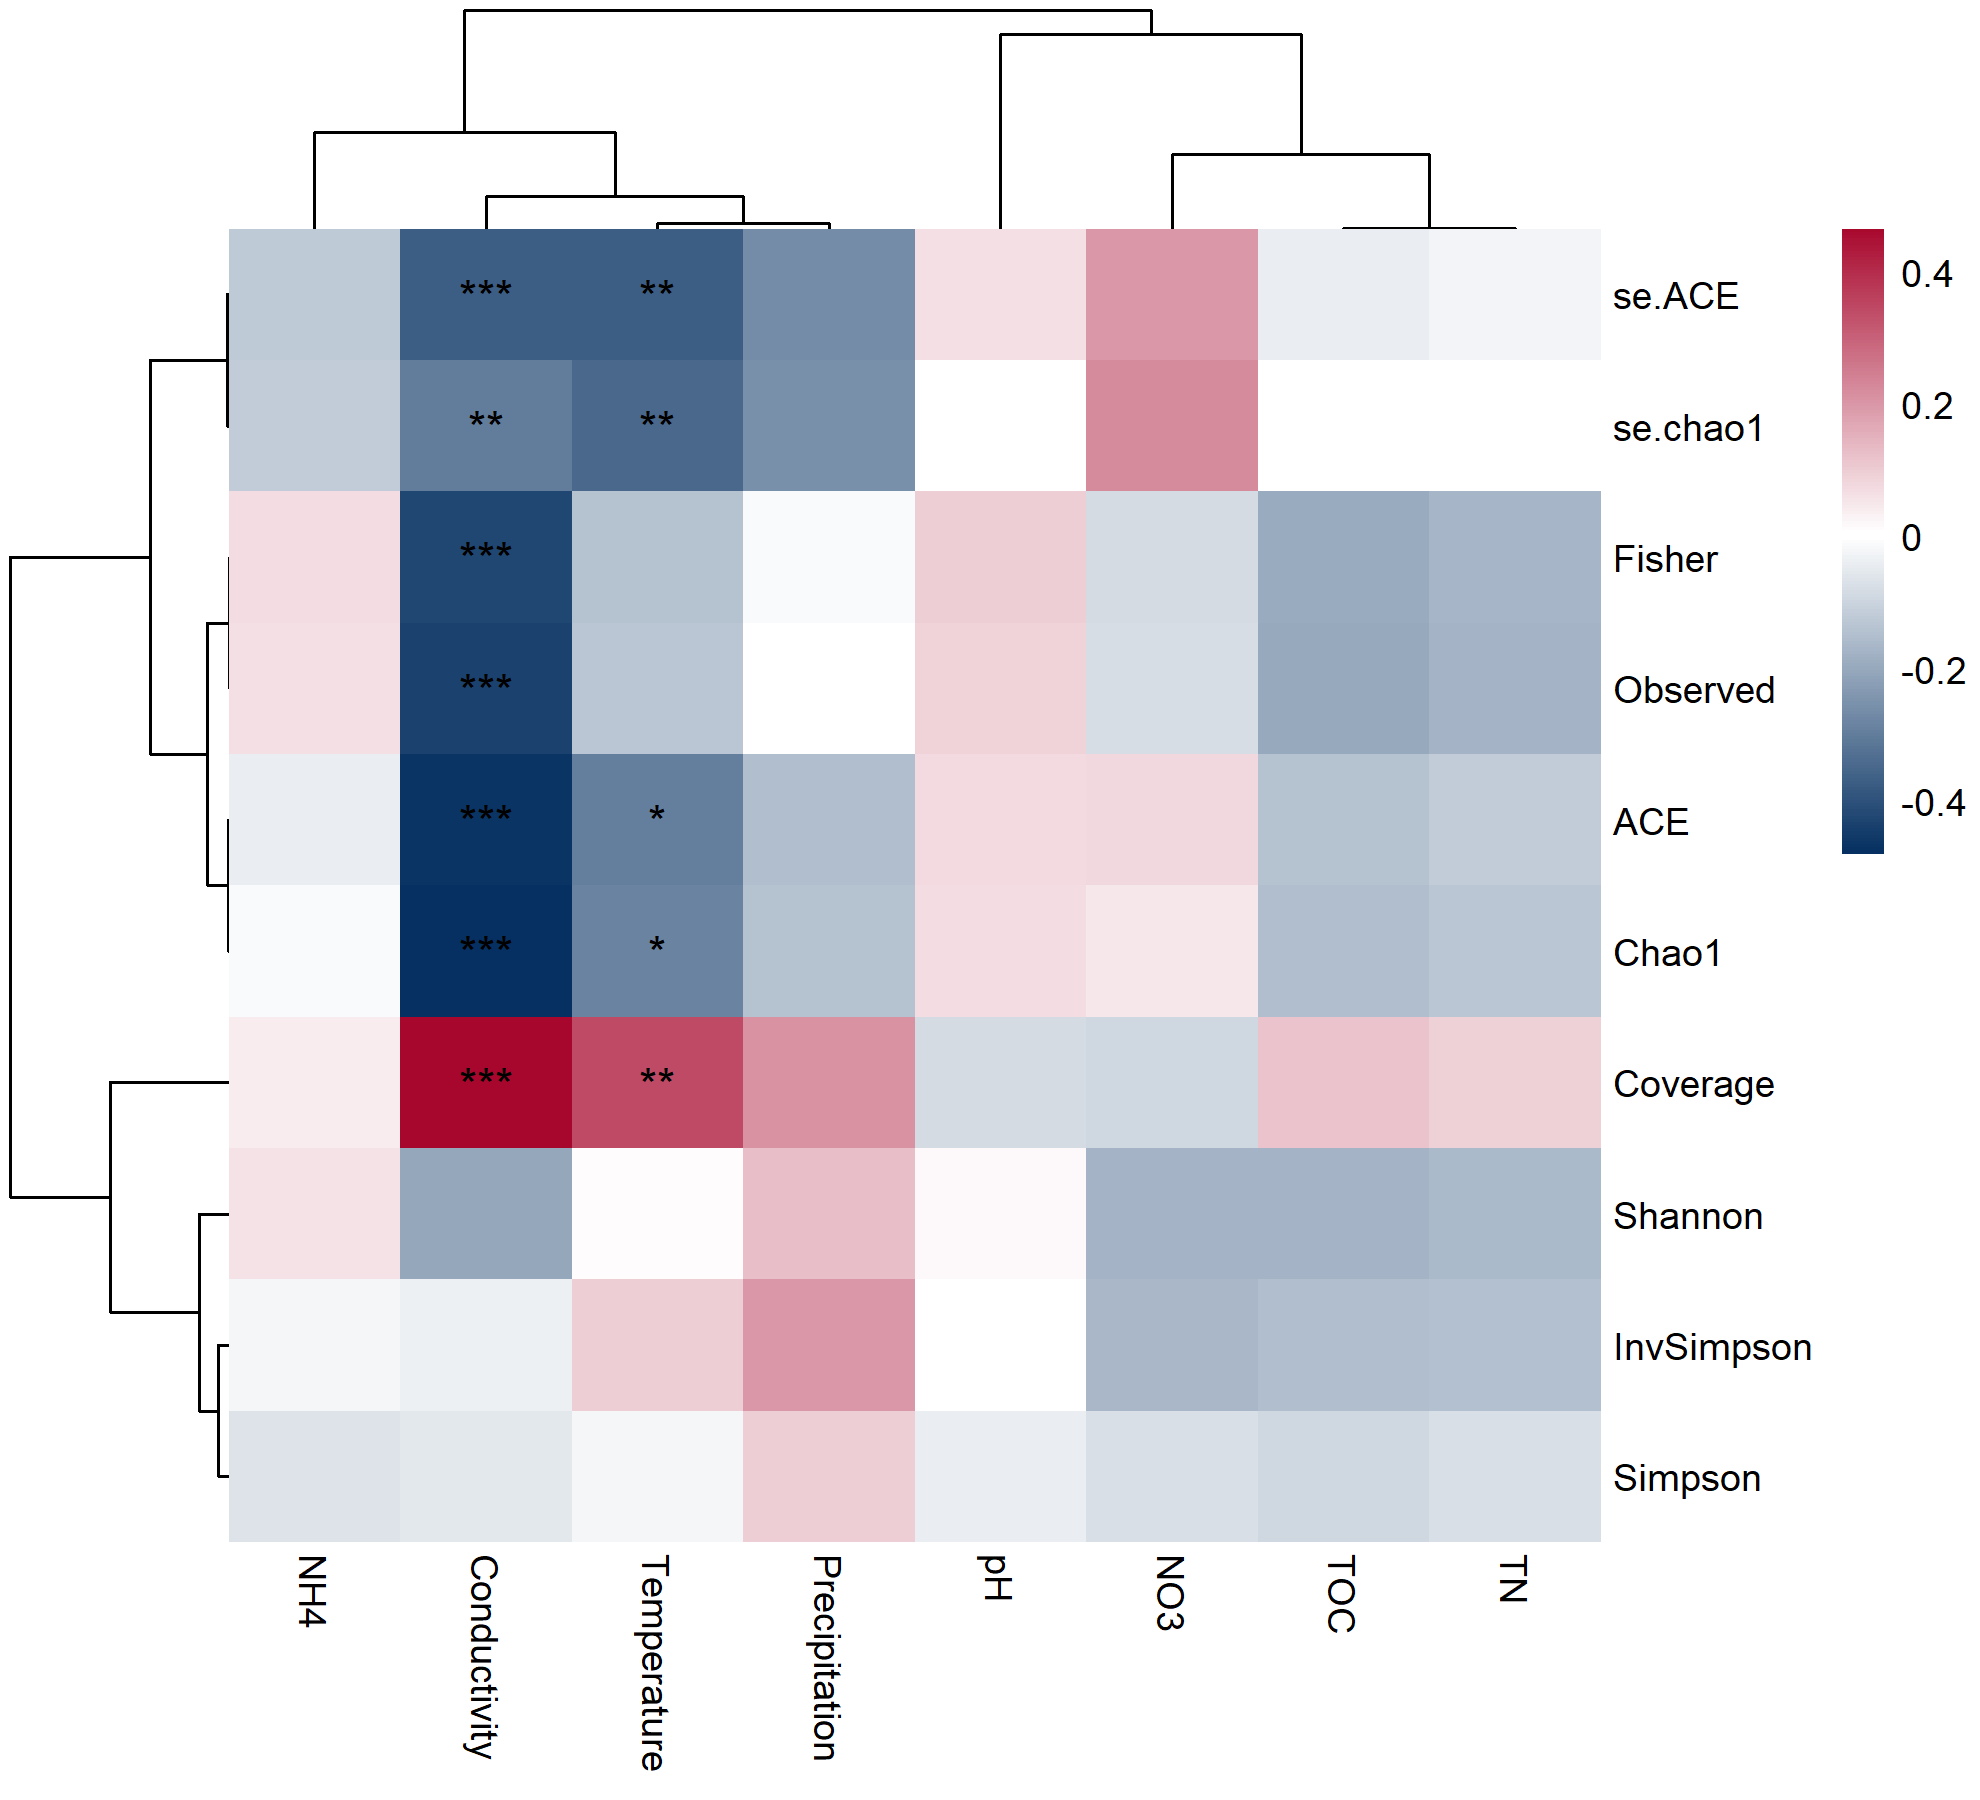
\includegraphics[width=600px]{Images/plot_corr_alpha_diversity} \end{center}

The function plot\_scatterfit() in trans\_env class is designed for the scatter plot, adding the fitted line and statistics.

\begin{Shaded}
\begin{Highlighting}[]
\CommentTok{\# use pH and bray{-}curtis distance}
\NormalTok{t1}\SpecialCharTok{$}\FunctionTok{plot\_scatterfit}\NormalTok{(}
    \AttributeTok{x =} \StringTok{"pH"}\NormalTok{, }
    \AttributeTok{y =}\NormalTok{ dataset}\SpecialCharTok{$}\NormalTok{beta\_diversity}\SpecialCharTok{$}\NormalTok{bray[}\FunctionTok{rownames}\NormalTok{(t1}\SpecialCharTok{$}\NormalTok{env\_data), }\FunctionTok{rownames}\NormalTok{(t1}\SpecialCharTok{$}\NormalTok{env\_data)], }
    \AttributeTok{alpha =}\NormalTok{ .}\DecValTok{1}\NormalTok{,}
    \AttributeTok{x\_axis\_title =} \StringTok{"Euclidean distance of pH"}\NormalTok{, }
    \AttributeTok{y\_axis\_title =} \StringTok{"Bray{-}Curtis distance"}\NormalTok{, }
    \AttributeTok{text\_x\_pos =} \DecValTok{4}\NormalTok{, }
    \AttributeTok{text\_y\_pos =}\NormalTok{ .}\DecValTok{4}\NormalTok{)}
\end{Highlighting}
\end{Shaded}

\begin{center}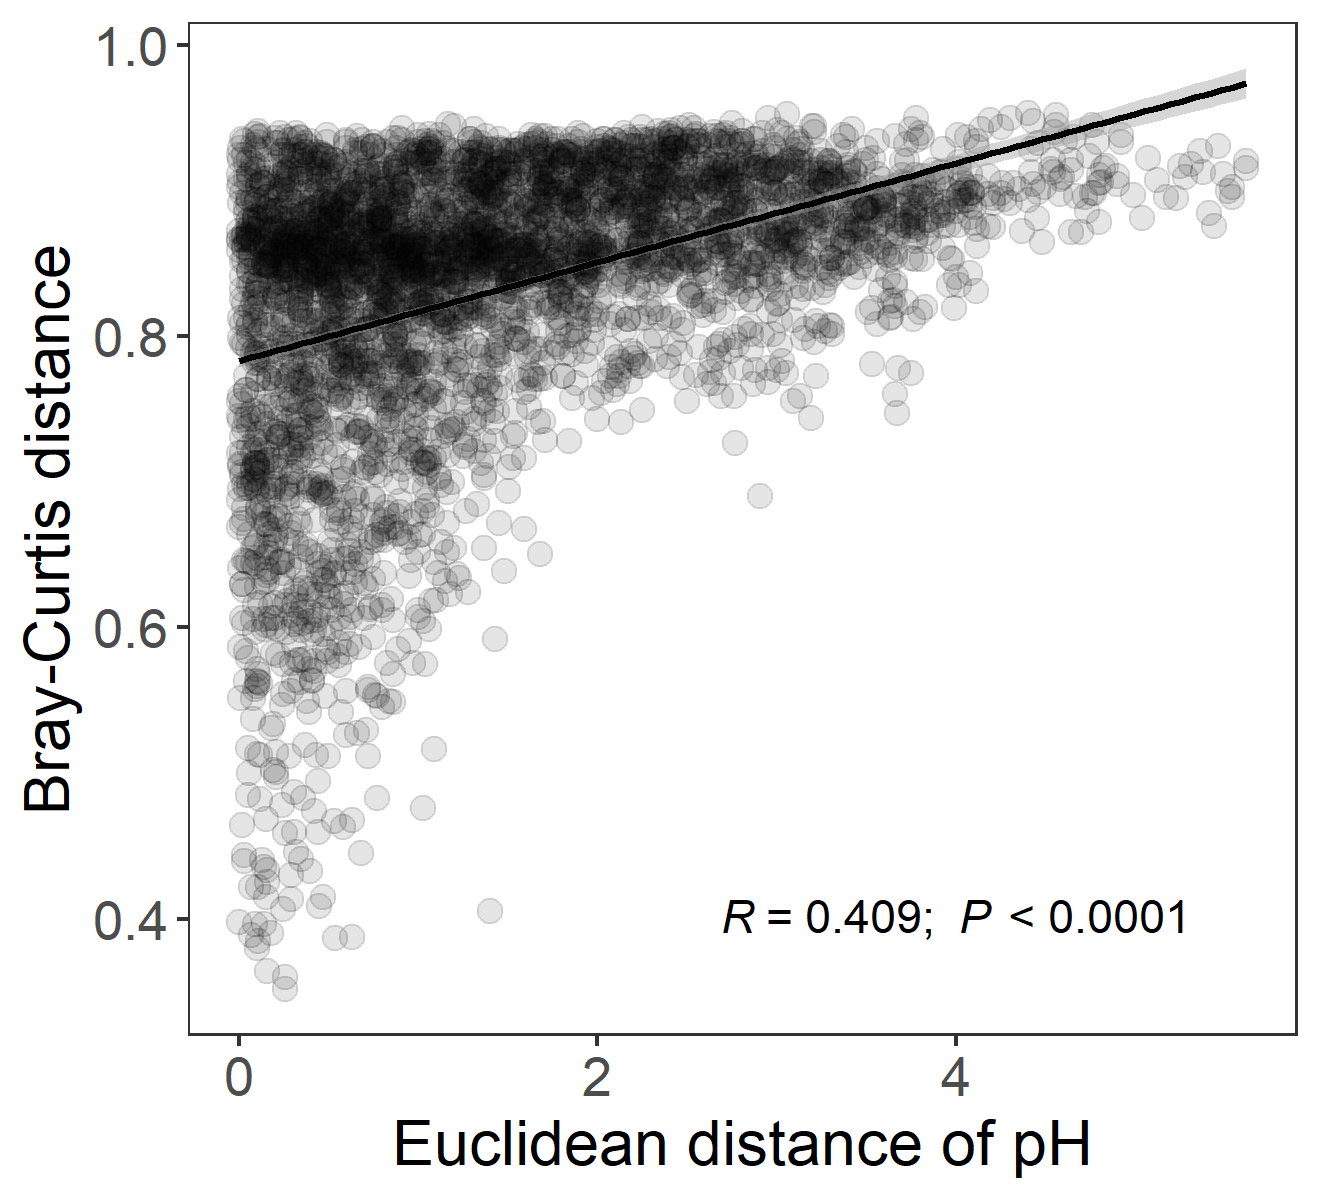
\includegraphics[width=550px]{Images/plot_scatterfit_pHbray} \end{center}

\hypertarget{trans_nullmodel-class}{%
\section{trans\_nullmodel class}\label{trans_nullmodel-class}}

In recent decades,
the integration of phylogenetic analysis and null model promotes the inference of niche and neutral influences on community assembly more powerfully
by adding a phylogeny dimension \citep{Webb_Phylogenies_2002, Stegen_Quantifying_2013}.
The trans\_nullmodel class provides an encapsulation, including the calculation of the phylogenetic signal,
beta mean pairwise phylogenetic distance (betaMPD), beta mean nearest taxon distance (betaMNTD),
beta nearest taxon index (betaNTI), beta net relatedness index (betaNRI) and Bray-Curtis-based Raup-Crick (RCbray).
The approach for phylogenetic signal analysis is based on the mantel correlogram \citep{Liu_Long_term_2017},
in which the change of phylogenetic signal is intuitional and clear compared to other approaches.
The algorithms of betaMNTD and betaMPD have been optimized to be faster than those in the picante package \citep{Picante_Kembel_2010}.
The combinations between RCbray and betaNTI (or betaNRI) can be used to infer the strength of each ecological process dominating the community assembly
under the specific hypothesis \citep{Stegen_Quantifying_2013}.
This can be achievable by the function cal\_process() to parse the percentage of each inferred process.
We first check the phylogenetic signal.

\begin{Shaded}
\begin{Highlighting}[]
\CommentTok{\# generate trans\_nullmodel object; use 1000 OTUs as example}
\NormalTok{t1 }\OtherTok{\textless{}{-}}\NormalTok{ trans\_nullmodel}\SpecialCharTok{$}\FunctionTok{new}\NormalTok{(dataset, }\AttributeTok{taxa\_number =} \DecValTok{1000}\NormalTok{, }\AttributeTok{add\_data =}\NormalTok{ env\_data\_16S)}
\end{Highlighting}
\end{Shaded}

\begin{Shaded}
\begin{Highlighting}[]
\CommentTok{\# use pH as the test variable}
\NormalTok{t1}\SpecialCharTok{$}\FunctionTok{cal\_mantel\_corr}\NormalTok{(}\AttributeTok{use\_env =} \StringTok{"pH"}\NormalTok{)}
\CommentTok{\# return t1$res\_mantel\_corr}
\CommentTok{\# plot the mantel correlogram}
\NormalTok{t1}\SpecialCharTok{$}\FunctionTok{plot\_mantel\_corr}\NormalTok{()}
\end{Highlighting}
\end{Shaded}

\begin{center}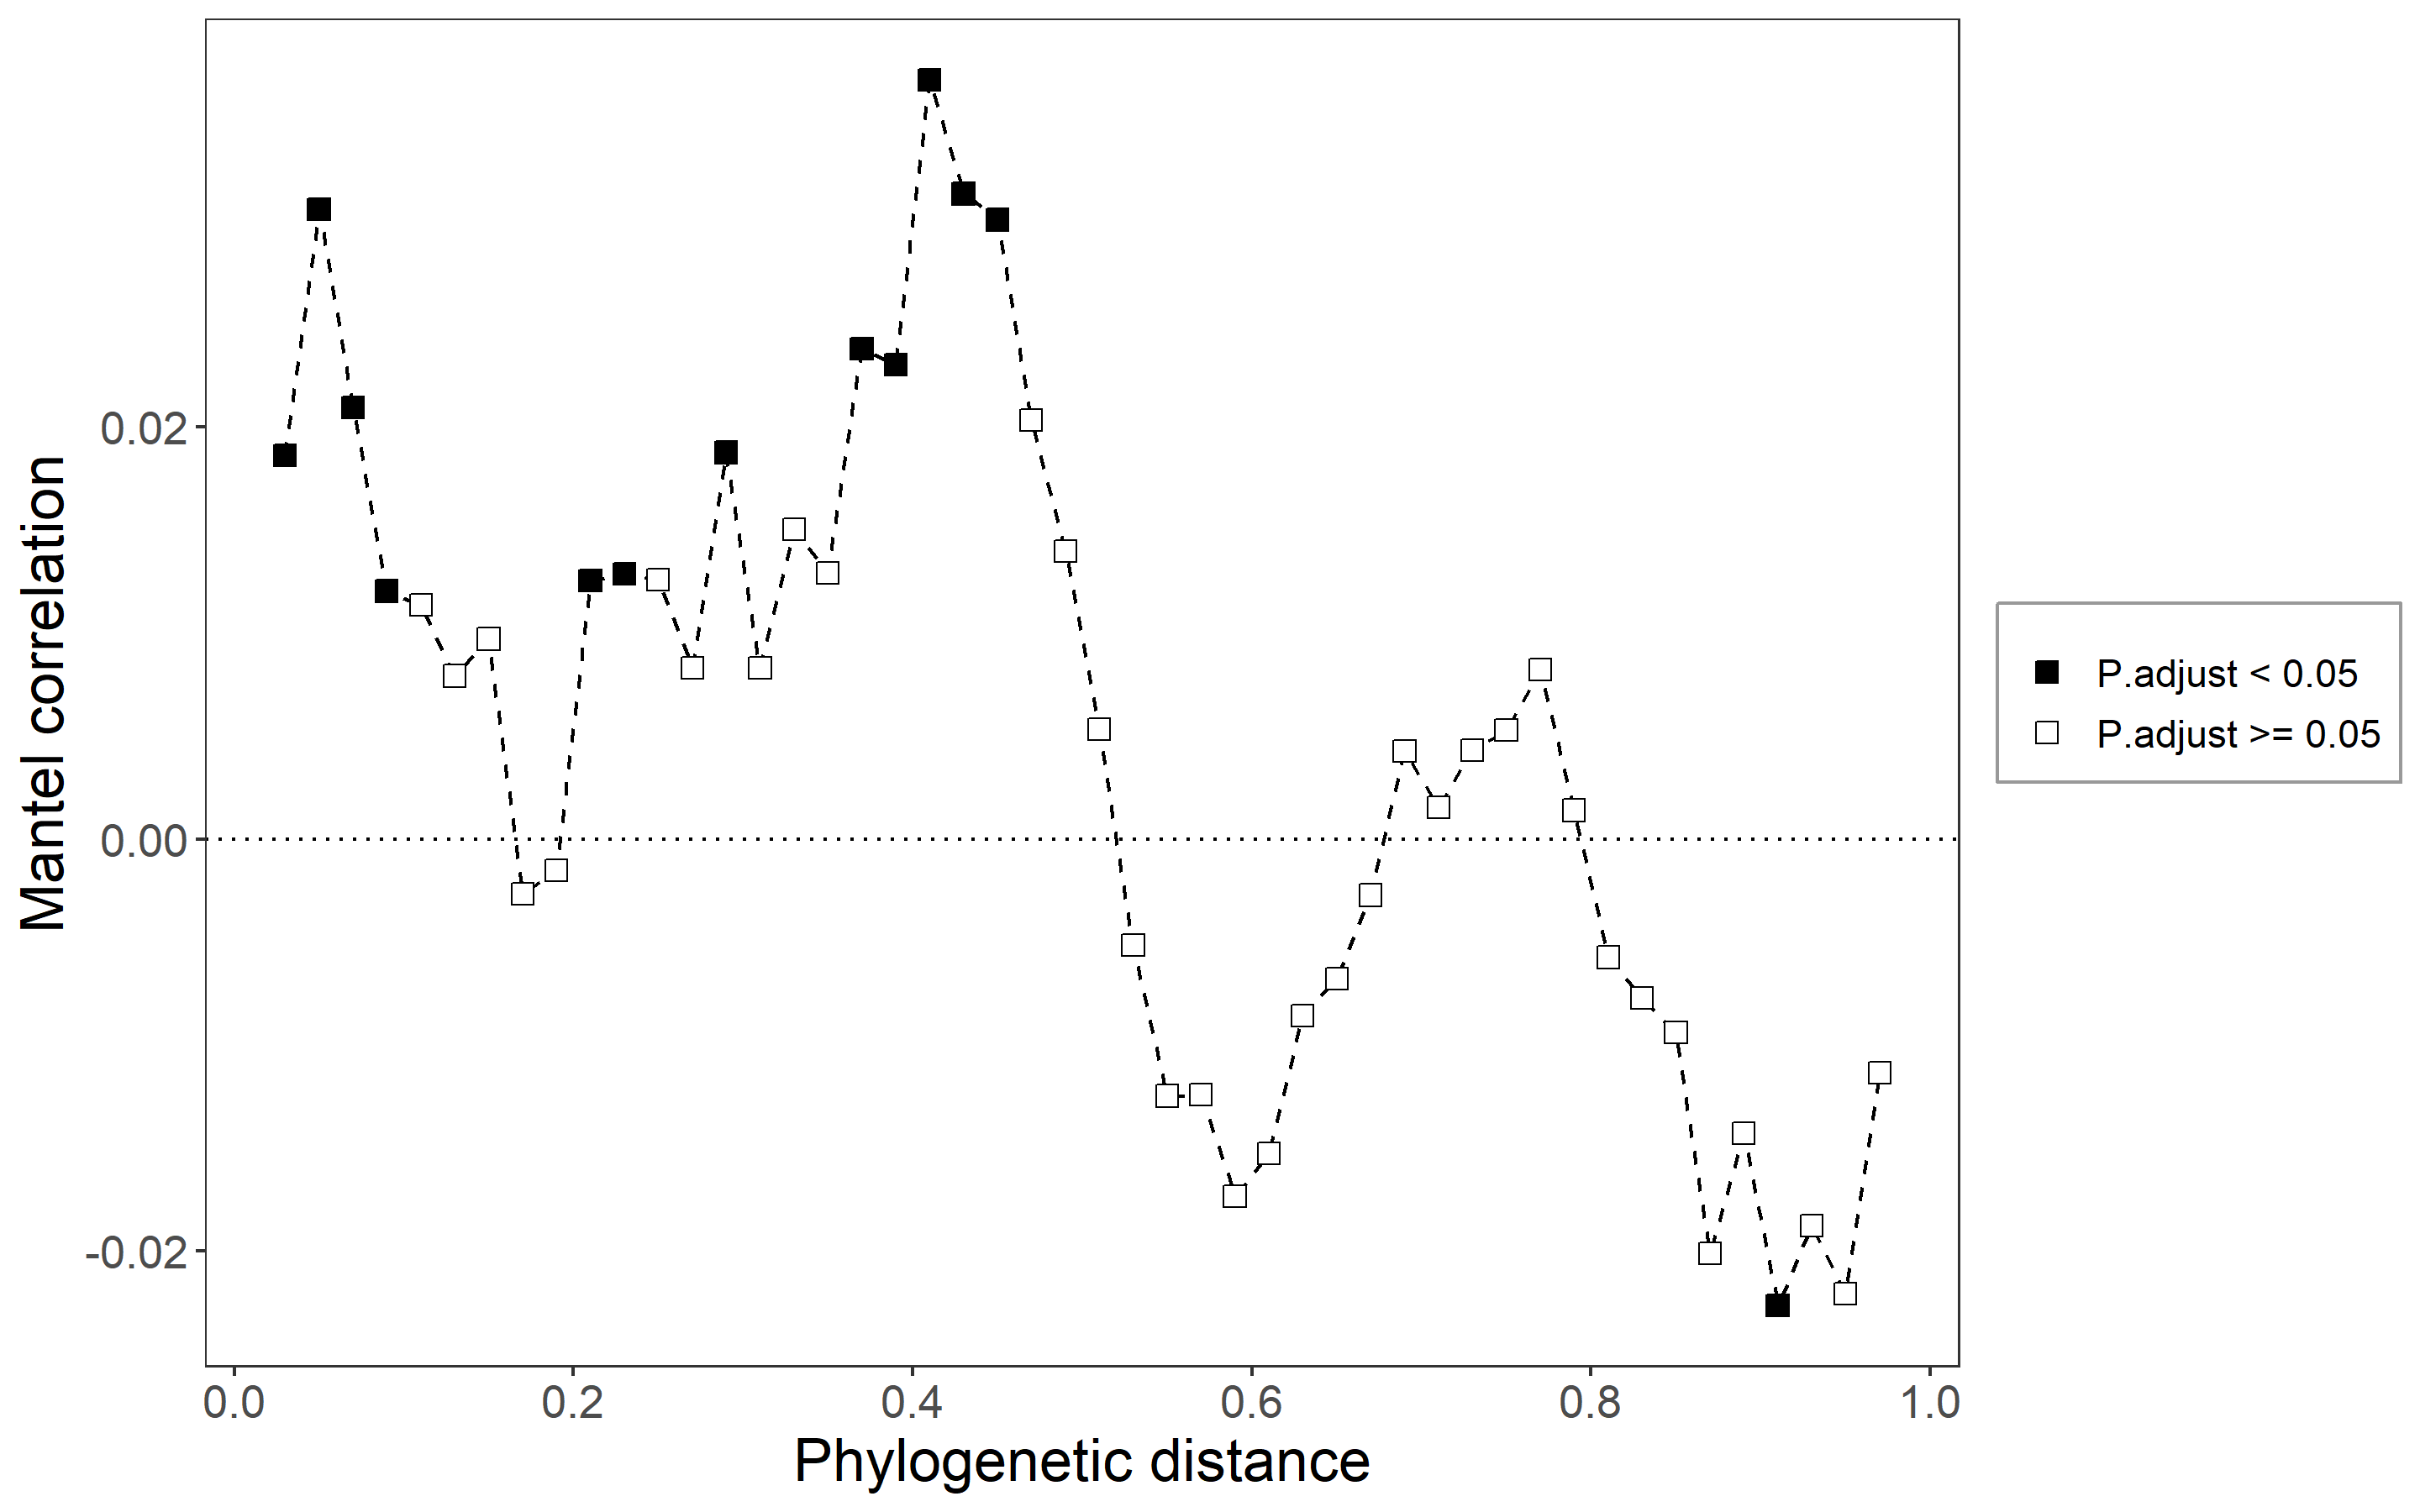
\includegraphics[width=600px]{Images/plot_mantel_corr} \end{center}

betaNRI(ses.betampd) is used to show the `basal' phylogenetic turnover\citep{Liu_Long_term_2017}.
Compared to betaNTI, it can capture more turnover information associated with the deep phylogeny.
It is noted that there are many null models with the development in the several decades.
In the trans\_nullmodel class, we randomized the phylogenetic relatedness of species.
This shuffling approach fix the observed levels of species α-diversity and β-diversity to
explore whether the observed phylogenetic turnover significantly differ from null model that phylogenetic relatedness among species are random.

\begin{Shaded}
\begin{Highlighting}[]
\CommentTok{\# null model run 500 times}
\NormalTok{t1}\SpecialCharTok{$}\FunctionTok{cal\_ses\_betampd}\NormalTok{(}\AttributeTok{runs=}\DecValTok{500}\NormalTok{, }\AttributeTok{abundance.weighted =} \ConstantTok{TRUE}\NormalTok{)}
\CommentTok{\# return t1$res\_ses\_betampd}
\end{Highlighting}
\end{Shaded}

If we want to plot the betaNRI, we can use plot\_group\_distance function in trans\_beta class.
For example, the results showed that the mean betaNRI of TW is extremely and significantly larger that those in CW and IW,
revealing that the basal phylogenetic turnover in TW is high.

\begin{Shaded}
\begin{Highlighting}[]
\CommentTok{\# add betaNRI matrix to beta\_diversity list}
\NormalTok{dataset}\SpecialCharTok{$}\NormalTok{beta\_diversity[[}\StringTok{"betaNRI"}\NormalTok{]] }\OtherTok{\textless{}{-}}\NormalTok{ t1}\SpecialCharTok{$}\NormalTok{res\_ses\_betampd}
\CommentTok{\# create trans\_beta class, use measure "betaNRI"}
\NormalTok{t2 }\OtherTok{\textless{}{-}}\NormalTok{ trans\_beta}\SpecialCharTok{$}\FunctionTok{new}\NormalTok{(}\AttributeTok{dataset =}\NormalTok{ dataset, }\AttributeTok{group =} \StringTok{"Group"}\NormalTok{, }\AttributeTok{measure =} \StringTok{"betaNRI"}\NormalTok{)}
\CommentTok{\# transform the distance for each group}
\NormalTok{t2}\SpecialCharTok{$}\FunctionTok{cal\_group\_distance}\NormalTok{()}
\CommentTok{\# plot the results}
\NormalTok{g1 }\OtherTok{\textless{}{-}}\NormalTok{ t2}\SpecialCharTok{$}\FunctionTok{plot\_group\_distance}\NormalTok{(}\AttributeTok{distance\_pair\_stat =} \ConstantTok{TRUE}\NormalTok{)}
\NormalTok{g1 }\SpecialCharTok{+} \FunctionTok{geom\_hline}\NormalTok{(}\AttributeTok{yintercept =} \SpecialCharTok{{-}}\DecValTok{2}\NormalTok{, }\AttributeTok{linetype =} \DecValTok{2}\NormalTok{) }\SpecialCharTok{+} \FunctionTok{geom\_hline}\NormalTok{(}\AttributeTok{yintercept =} \DecValTok{2}\NormalTok{, }\AttributeTok{linetype =} \DecValTok{2}\NormalTok{)}
\end{Highlighting}
\end{Shaded}

\begin{center}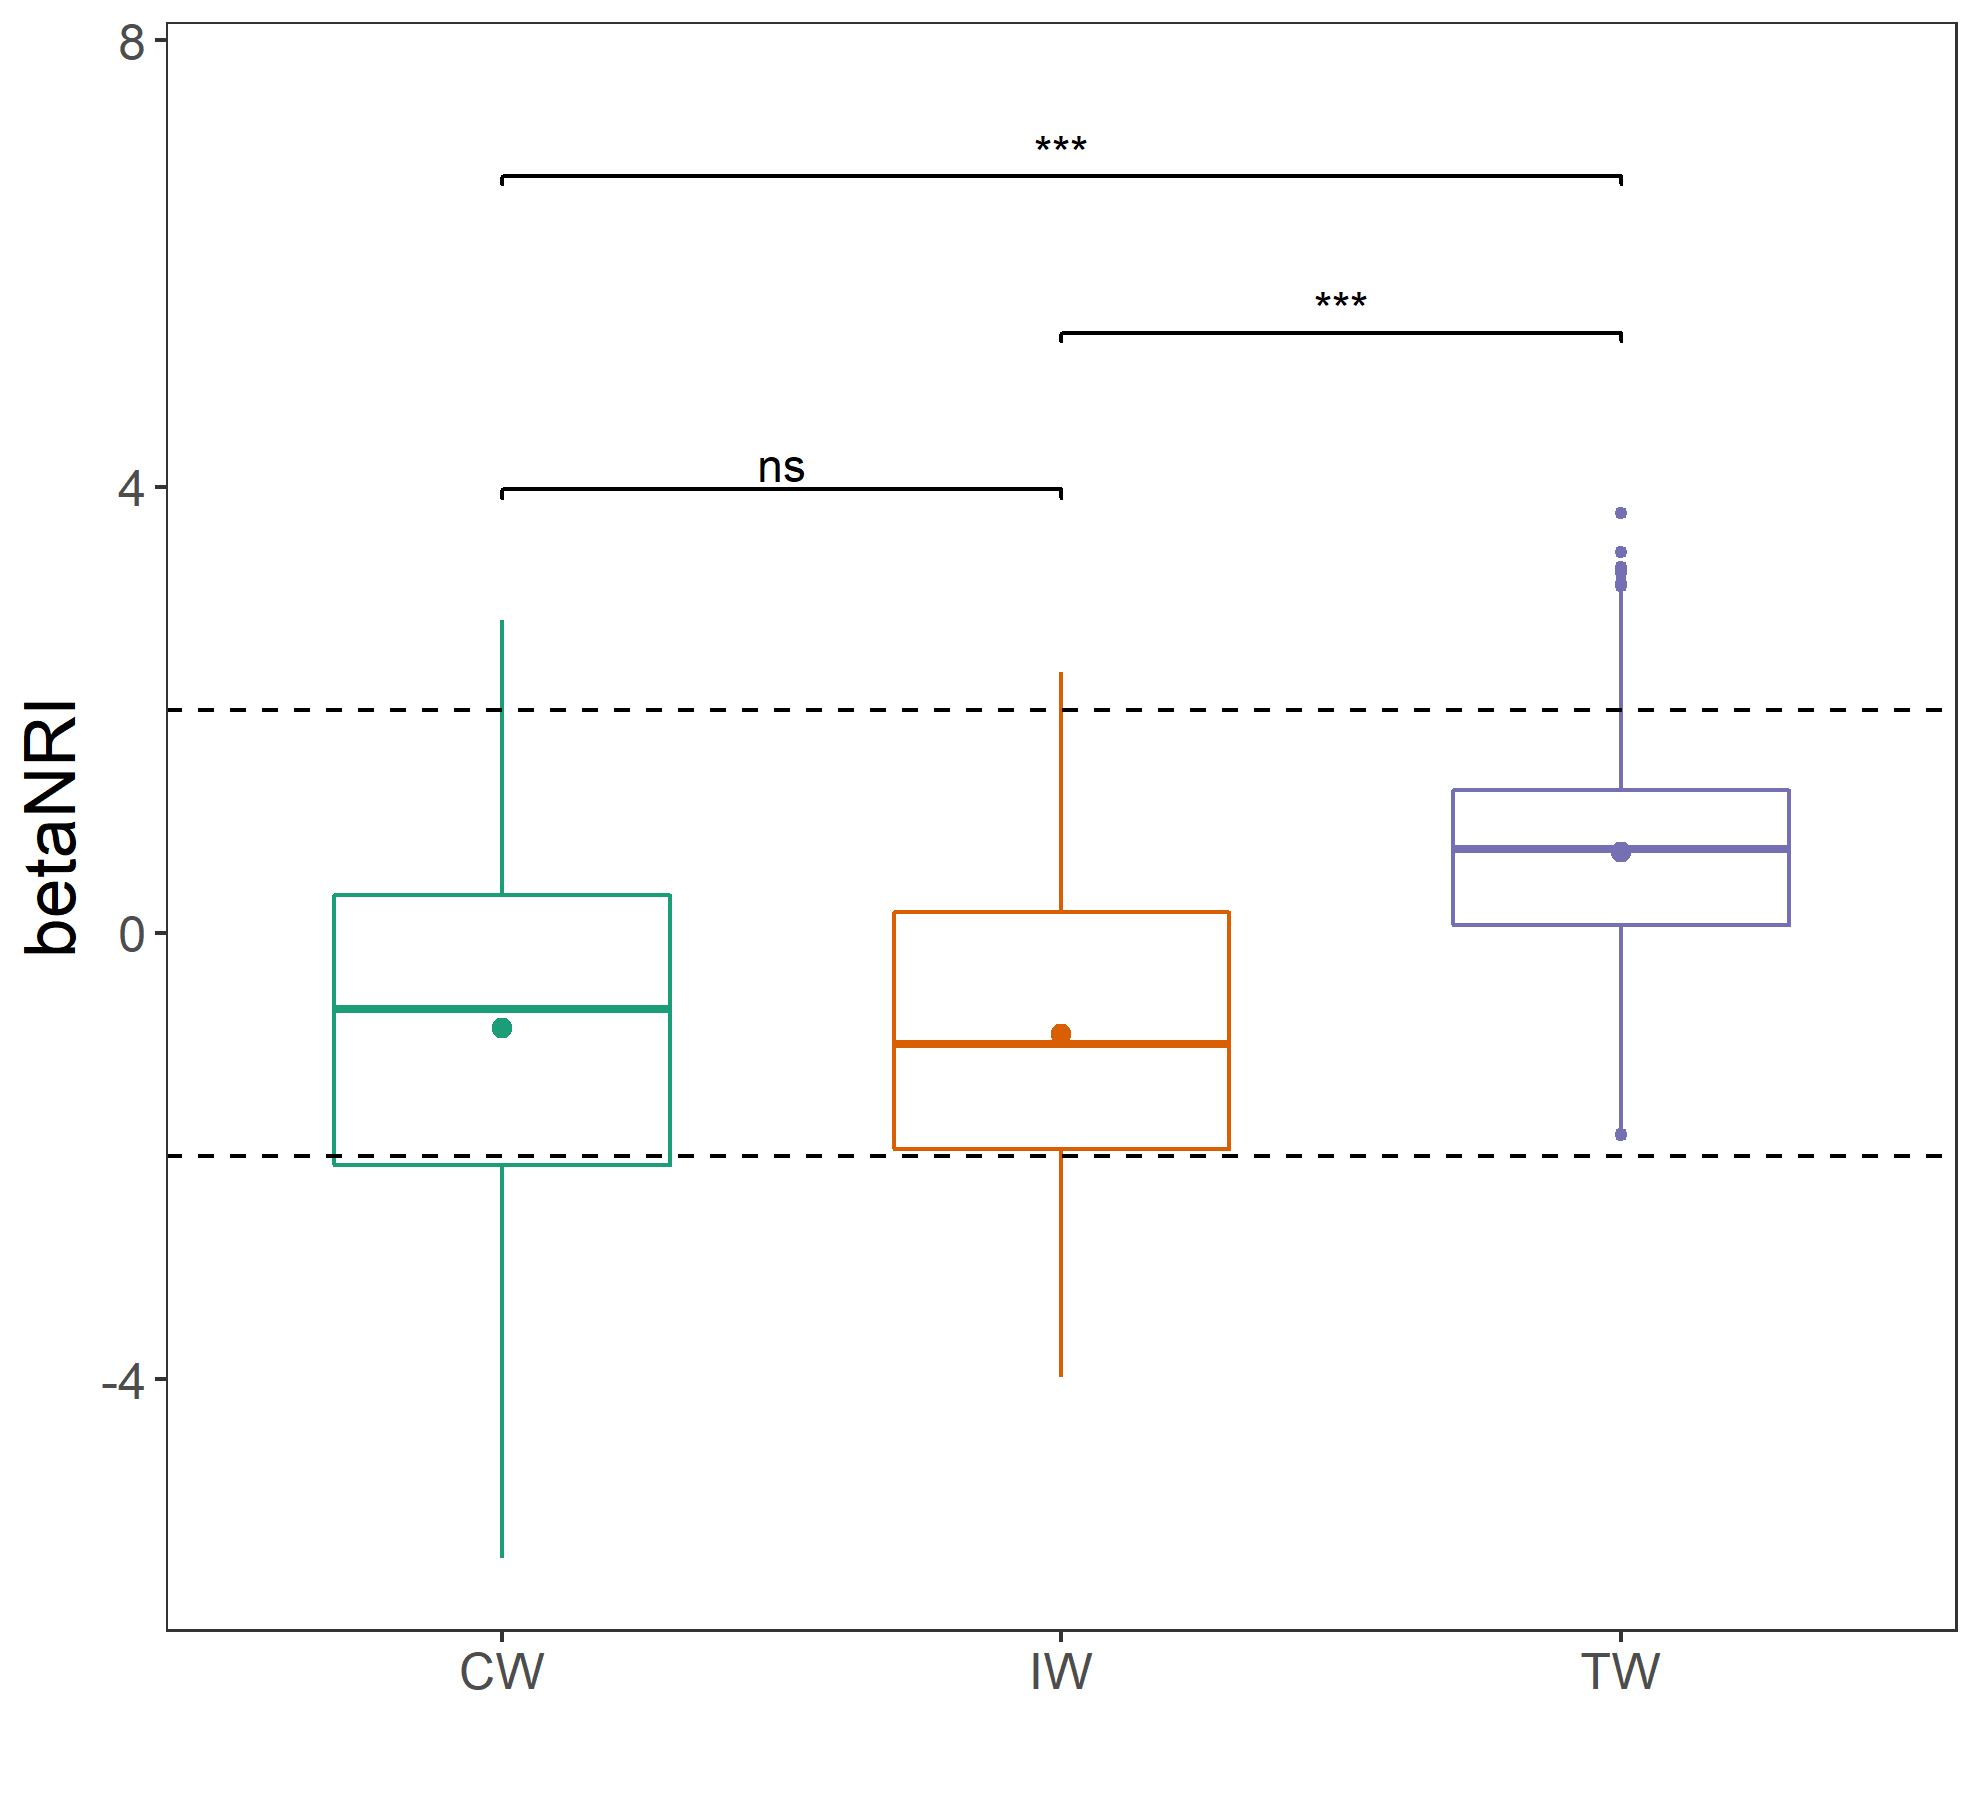
\includegraphics[width=550px]{Images/plot_betaNRI_one_dataset} \end{center}

Sometimes, if you want to perform null model analysis for each group individually, such as one group as one species pool,
you can calculate the results for each group, respectively.
We can find that, when we perform betaNRI for each group respectively,
mean betaNRI between CW and TW are not significantly different, and they are both significantly higher than that in IW,
revealing that the strength of variable selection in CW and TW may be similar under the condition that each area is considered as a specific species pool.

\begin{Shaded}
\begin{Highlighting}[]
\CommentTok{\# we create a list to store the trans\_nullmodel results.}
\NormalTok{sesbeta\_each }\OtherTok{\textless{}{-}} \FunctionTok{list}\NormalTok{()}
\NormalTok{group\_col }\OtherTok{\textless{}{-}} \StringTok{"Group"}
\NormalTok{all\_groups }\OtherTok{\textless{}{-}} \FunctionTok{unique}\NormalTok{(dataset}\SpecialCharTok{$}\NormalTok{sample\_table[, group\_col])}
\CommentTok{\# calculate for each group, respectively}
\ControlFlowTok{for}\NormalTok{(i }\ControlFlowTok{in}\NormalTok{ all\_groups)\{}
    \CommentTok{\# like the above operation, but need provide \textquotesingle{}group\textquotesingle{} and \textquotesingle{}select\_group\textquotesingle{}}
\NormalTok{    test }\OtherTok{\textless{}{-}}\NormalTok{ trans\_nullmodel}\SpecialCharTok{$}\FunctionTok{new}\NormalTok{(dataset, }\AttributeTok{group =}\NormalTok{ group\_col, }\AttributeTok{select\_group =}\NormalTok{ i, }\AttributeTok{taxa\_number =} \DecValTok{1000}\NormalTok{, }\AttributeTok{add\_data =}\NormalTok{ env\_data\_16S)}
\NormalTok{    test}\SpecialCharTok{$}\FunctionTok{cal\_ses\_betampd}\NormalTok{(}\AttributeTok{runs =} \DecValTok{500}\NormalTok{, }\AttributeTok{abundance.weighted =} \ConstantTok{TRUE}\NormalTok{)}
\NormalTok{    sesbeta\_each[[i]] }\OtherTok{\textless{}{-}}\NormalTok{ test}\SpecialCharTok{$}\NormalTok{res\_ses\_betampd}
\NormalTok{\}}
\CommentTok{\# merge and reshape to generate one symmetrical matrix}
\NormalTok{test }\OtherTok{\textless{}{-}} \FunctionTok{lapply}\NormalTok{(sesbeta\_each, melt) }\SpecialCharTok{\%\textgreater{}\%} \FunctionTok{do.call}\NormalTok{(rbind, .) }\SpecialCharTok{\%\textgreater{}\%}
\NormalTok{    reshape2}\SpecialCharTok{::}\FunctionTok{dcast}\NormalTok{(., Var1}\SpecialCharTok{\textasciitilde{}}\NormalTok{Var2, }\AttributeTok{value.var =} \StringTok{"value"}\NormalTok{) }\SpecialCharTok{\%\textgreater{}\%} \StringTok{\textasciigrave{}}\AttributeTok{row.names\textless{}{-}}\StringTok{\textasciigrave{}}\NormalTok{(.[,}\DecValTok{1}\NormalTok{]) }\SpecialCharTok{\%\textgreater{}\%}\NormalTok{ .[, }\SpecialCharTok{{-}}\DecValTok{1}\NormalTok{, drop }\OtherTok{=} \ConstantTok{FALSE}\NormalTok{]}
\CommentTok{\# like the above operation}
\NormalTok{dataset}\SpecialCharTok{$}\NormalTok{beta\_diversity[[}\StringTok{"betaNRI"}\NormalTok{]] }\OtherTok{\textless{}{-}}\NormalTok{ test}
\NormalTok{t2 }\OtherTok{\textless{}{-}}\NormalTok{ trans\_beta}\SpecialCharTok{$}\FunctionTok{new}\NormalTok{(}\AttributeTok{dataset =}\NormalTok{ dataset, }\AttributeTok{group =} \StringTok{"Group"}\NormalTok{, }\AttributeTok{measure =} \StringTok{"betaNRI"}\NormalTok{)}
\NormalTok{t2}\SpecialCharTok{$}\FunctionTok{cal\_group\_distance}\NormalTok{()}
\NormalTok{g1 }\OtherTok{\textless{}{-}}\NormalTok{ t2}\SpecialCharTok{$}\FunctionTok{plot\_group\_distance}\NormalTok{(}\AttributeTok{distance\_pair\_stat =} \ConstantTok{TRUE}\NormalTok{)}
\NormalTok{g1 }\SpecialCharTok{+} \FunctionTok{geom\_hline}\NormalTok{(}\AttributeTok{yintercept =} \SpecialCharTok{{-}}\DecValTok{2}\NormalTok{, }\AttributeTok{linetype =} \DecValTok{2}\NormalTok{) }\SpecialCharTok{+} \FunctionTok{geom\_hline}\NormalTok{(}\AttributeTok{yintercept =} \DecValTok{2}\NormalTok{, }\AttributeTok{linetype =} \DecValTok{2}\NormalTok{)}
\end{Highlighting}
\end{Shaded}

\begin{center}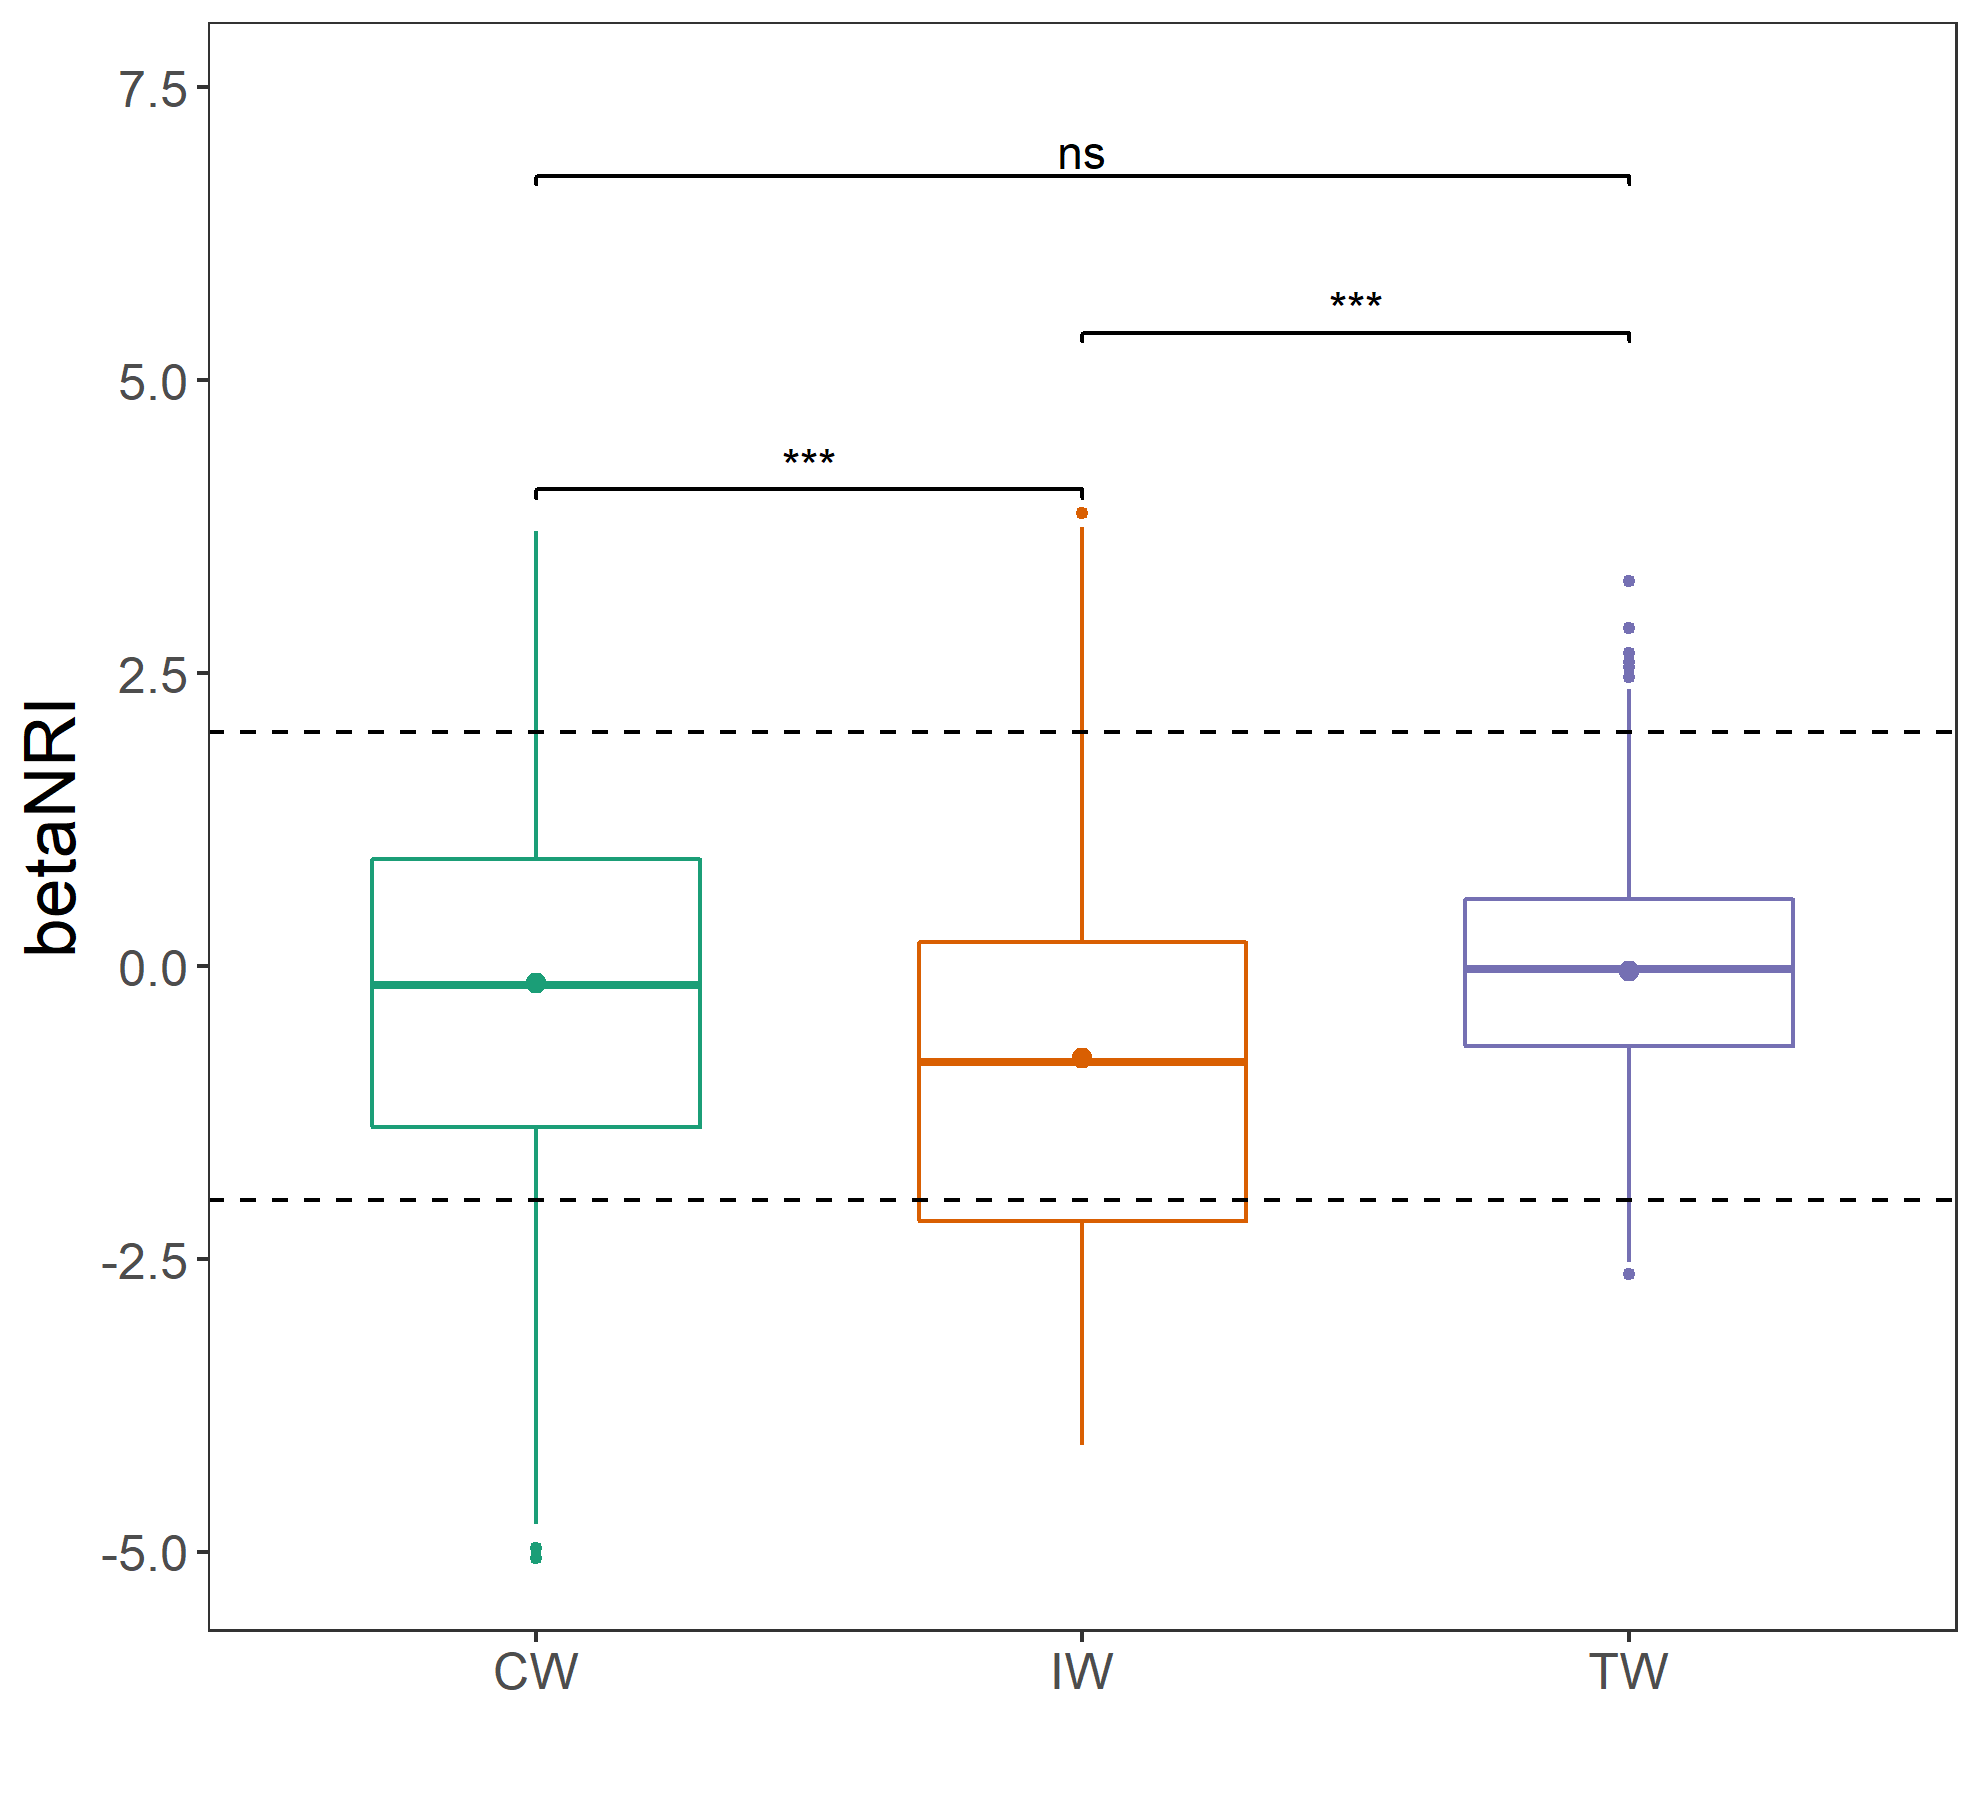
\includegraphics[width=550px]{Images/plot_betaNRI_each_dataset} \end{center}

BetaNTI(ses.betamntd) can be used to indicate the phylogenetic terminal turnover \citep{Stegen_Quantifying_2013}.

\begin{Shaded}
\begin{Highlighting}[]
\CommentTok{\# null model run 500 times}
\NormalTok{t1}\SpecialCharTok{$}\FunctionTok{cal\_ses\_betamntd}\NormalTok{(}\AttributeTok{runs=}\DecValTok{500}\NormalTok{, }\AttributeTok{abundance.weighted =} \ConstantTok{TRUE}\NormalTok{)}
\CommentTok{\# return t1$res\_ses\_betamntd}
\end{Highlighting}
\end{Shaded}

\begin{longtable}[]{@{}
  >{\centering\arraybackslash}p{(\columnwidth - 10\tabcolsep) * \real{0.12}}
  >{\centering\arraybackslash}p{(\columnwidth - 10\tabcolsep) * \real{0.12}}
  >{\centering\arraybackslash}p{(\columnwidth - 10\tabcolsep) * \real{0.12}}
  >{\centering\arraybackslash}p{(\columnwidth - 10\tabcolsep) * \real{0.12}}
  >{\centering\arraybackslash}p{(\columnwidth - 10\tabcolsep) * \real{0.12}}
  >{\centering\arraybackslash}p{(\columnwidth - 10\tabcolsep) * \real{0.12}}@{}}
\toprule
~ & S1 & S2 & S3 & S4 & S5 \\
\midrule
\endhead
\textbf{S1} & 0 & -6.554 & -6.563 & -6.308 & -6.153 \\
\textbf{S2} & -6.554 & 0 & -6.678 & -6.675 & -6.124 \\
\textbf{S3} & -6.563 & -6.678 & 0 & -6.544 & -6.46 \\
\textbf{S4} & -6.308 & -6.675 & -6.544 & 0 & -6.356 \\
\textbf{S5} & -6.153 & -6.124 & -6.46 & -6.356 & 0 \\
\bottomrule
\end{longtable}

RCbray (Bray-Curtis-based Raup-Crick) can be calculated using function cal\_rcbray()
to assess whether the compositional turnover was governed primarily by drift \citep{Chase_null_2011}.
We applied null model to simulate species distribution by randomly sampling individuals from each
species pool with preserving species occurrence frequency and sample species richness \citep{Liu_Long_term_2017}.

\begin{Shaded}
\begin{Highlighting}[]
\CommentTok{\# result stored in t1$res\_rcbray}
\NormalTok{t1}\SpecialCharTok{$}\FunctionTok{cal\_rcbray}\NormalTok{(}\AttributeTok{runs =} \DecValTok{1000}\NormalTok{)}
\CommentTok{\# return t1$res\_rcbray}
\end{Highlighting}
\end{Shaded}

As an example, we also calculate the proportion of the inferred processes on the community assembly as shown in the references \citep{Stegen_Quantifying_2013, Liu_Long_term_2017}.
In the example, the fraction of pairwise comparisons with significant betaNTI values (\textbar βNTI\textbar{} \textgreater{} 2) is the estimated influence of Selection;
βNTI \textgreater{} 2 represents the heterogeneous selection; βNTI \textless{} -2 represents the homogeneous selection.
The value of RCbray characterizes the magnitude of deviation between observed Bray--Curtis and Bray--Curtis expected under the randomization;
a value of \textbar RCbray\textbar{} \textgreater{} 0.95 was considered significant.
The fraction of all pairwise comparisons with \textbar βNTI\textbar{} \textless{} 2 and RCbray \textgreater{} +0.95 was taken as the influence of Dispersal Limitation combined with Drift.
The fraction of all pairwise comparisons with \textbar βNTI\textbar{} \textless{} 2 and RCbray \textless{} -0.95 was taken as an estimate for the influence of Homogenizing Dispersal.
The fraction of all pairwise comparisons with \textbar βNTI\textbar{} \textless{} 2 and \textbar RCbray\textbar{} \textless{} 0.95 estimates the influence of Drift acting alone.

\begin{Shaded}
\begin{Highlighting}[]
\CommentTok{\# use betaNTI and rcbray to evaluate processes}
\NormalTok{t1}\SpecialCharTok{$}\FunctionTok{cal\_process}\NormalTok{(}\AttributeTok{use\_betamntd =} \ConstantTok{TRUE}\NormalTok{)}
\end{Highlighting}
\end{Shaded}

\begin{verbatim}
## The result is stored in object$res_process ...
\end{verbatim}

\begin{Shaded}
\begin{Highlighting}[]
\CommentTok{\# return t1$res\_process}
\end{Highlighting}
\end{Shaded}

\begin{Shaded}
\begin{Highlighting}[]
\NormalTok{t1}\SpecialCharTok{$}\NormalTok{res\_process}
\end{Highlighting}
\end{Shaded}

\begin{longtable}[]{@{}
  >{\centering\arraybackslash}p{(\columnwidth - 2\tabcolsep) * \real{0.33}}
  >{\centering\arraybackslash}p{(\columnwidth - 2\tabcolsep) * \real{0.18}}@{}}
\toprule
process & percentage \\
\midrule
\endhead
variable selection & 3.995 \\
homogeneous selection & 48.34 \\
dispersal limitation & 0.02497 \\
homogeneous dispersal & 8.539 \\
drift & 39.1 \\
\bottomrule
\end{longtable}

\hypertarget{trans_network-class}{%
\section{trans\_network class}\label{trans_network-class}}

 Network is a frequently used approach to study the co-occurrence patterns in microbial ecology\citep{Deng_Molecular_2012, Faust_Microbial_2012, Coyte_Theecology_2015}.
In this part, we describe all the core contents in the trans\_network class.
The network construction approaches can be classified into two types: correlation-based and non correlation-based.
Several approaches can be used to calculate correlations and significances.

We first introduce the correlation-based network. The parameter cal\_cor in trans\_network is used for selecting the correlation calculation method.

\begin{Shaded}
\begin{Highlighting}[]
\CommentTok{\# Use R base cor.test, slow}
\NormalTok{t1 }\OtherTok{\textless{}{-}}\NormalTok{ trans\_network}\SpecialCharTok{$}\FunctionTok{new}\NormalTok{(}\AttributeTok{dataset =}\NormalTok{ dataset, }\AttributeTok{cal\_cor =} \StringTok{"base"}\NormalTok{, }\AttributeTok{taxa\_level =} \StringTok{"OTU"}\NormalTok{, }\AttributeTok{filter\_thres =} \FloatTok{0.0001}\NormalTok{, }\AttributeTok{cor\_method =} \StringTok{"spearman"}\NormalTok{)}
\CommentTok{\# return t1$res\_cor\_p list; one table: correlation; another: p value}
\end{Highlighting}
\end{Shaded}

\begin{Shaded}
\begin{Highlighting}[]
\CommentTok{\# SparCC method, require SpiecEasi package}
\CommentTok{\# SparCC is very slow, so consider filtering more species with low abundance}
\NormalTok{t1 }\OtherTok{\textless{}{-}}\NormalTok{ trans\_network}\SpecialCharTok{$}\FunctionTok{new}\NormalTok{(}\AttributeTok{dataset =}\NormalTok{ dataset, }\AttributeTok{cal\_cor =} \StringTok{"SparCC"}\NormalTok{, }\AttributeTok{taxa\_level =} \StringTok{"OTU"}\NormalTok{, }\AttributeTok{filter\_thres =} \FloatTok{0.001}\NormalTok{, }\AttributeTok{SparCC\_simu\_num =} \DecValTok{100}\NormalTok{)}
\end{Highlighting}
\end{Shaded}

\begin{Shaded}
\begin{Highlighting}[]
\CommentTok{\# When the OTU number is large, use R WGCNA package to replace R base to calculate correlations}
\CommentTok{\# require WGCNA package}
\NormalTok{t1 }\OtherTok{\textless{}{-}}\NormalTok{ trans\_network}\SpecialCharTok{$}\FunctionTok{new}\NormalTok{(}\AttributeTok{dataset =}\NormalTok{ dataset, }\AttributeTok{cal\_cor =} \StringTok{"WGCNA"}\NormalTok{, }\AttributeTok{taxa\_level =} \StringTok{"OTU"}\NormalTok{, }\AttributeTok{filter\_thres =} \FloatTok{0.0001}\NormalTok{, }\AttributeTok{cor\_method =} \StringTok{"spearman"}\NormalTok{)}
\end{Highlighting}
\end{Shaded}

The parameter COR\_cut can be used to select the correlation threshold.
Furthermore, COR\_optimization = TRUE represent using RMT theory to find the optimized correlation threshold instead of the COR\_cut\citep{Deng_Molecular_2012}.

\begin{Shaded}
\begin{Highlighting}[]
\CommentTok{\# construct network; require igraph package}
\NormalTok{t1}\SpecialCharTok{$}\FunctionTok{cal\_network}\NormalTok{(}\AttributeTok{p\_thres =} \FloatTok{0.01}\NormalTok{, }\AttributeTok{COR\_optimization =} \ConstantTok{TRUE}\NormalTok{)}
\CommentTok{\# return t1$res\_network}
\end{Highlighting}
\end{Shaded}

\begin{Shaded}
\begin{Highlighting}[]
\CommentTok{\# use arbitrary coefficient threshold to contruct network}
\NormalTok{t1}\SpecialCharTok{$}\FunctionTok{cal\_network}\NormalTok{(}\AttributeTok{p\_thres =} \FloatTok{0.01}\NormalTok{, }\AttributeTok{COR\_cut =} \FloatTok{0.7}\NormalTok{)}
\end{Highlighting}
\end{Shaded}

\begin{Shaded}
\begin{Highlighting}[]
\CommentTok{\# add modules in the network}
\NormalTok{t1}\SpecialCharTok{$}\FunctionTok{cal\_module}\NormalTok{()}
\end{Highlighting}
\end{Shaded}

\begin{Shaded}
\begin{Highlighting}[]
\CommentTok{\# save network}
\CommentTok{\# open the gexf file using Gephi(https://gephi.org/)}
\CommentTok{\# require rgexf package}
\NormalTok{t1}\SpecialCharTok{$}\FunctionTok{save\_network}\NormalTok{(}\AttributeTok{filepath =} \StringTok{"network.gexf"}\NormalTok{)}
\end{Highlighting}
\end{Shaded}

We plot the network and present the node colors according to the calculated modules in Gephi.

\begin{center}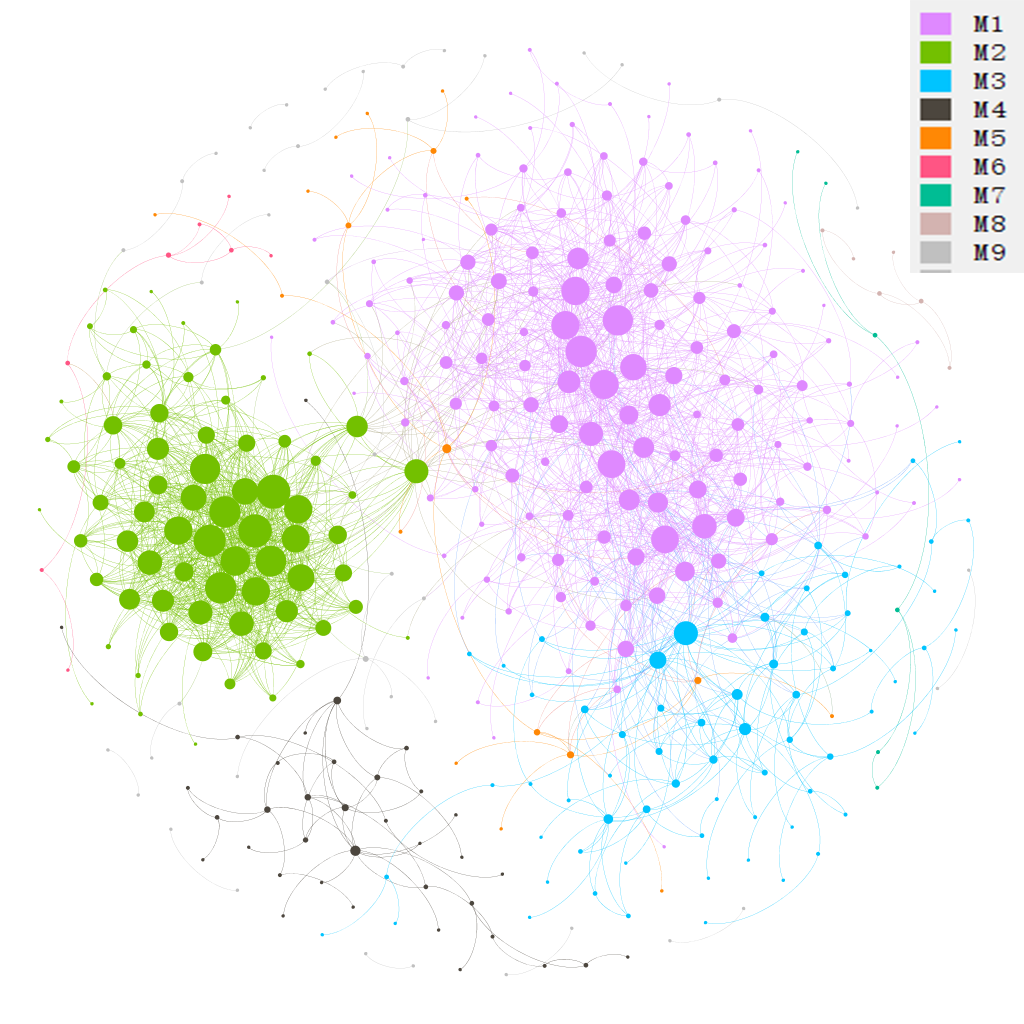
\includegraphics[width=550px]{Images/network1_spearman} \end{center}

Now, we show the node colors with the Phylum information and the edges colors with the positive and negative correlations.
All the data used has been stored in the network.gexf file, including modules classifications, Phylum information and edges classifications.

\begin{center}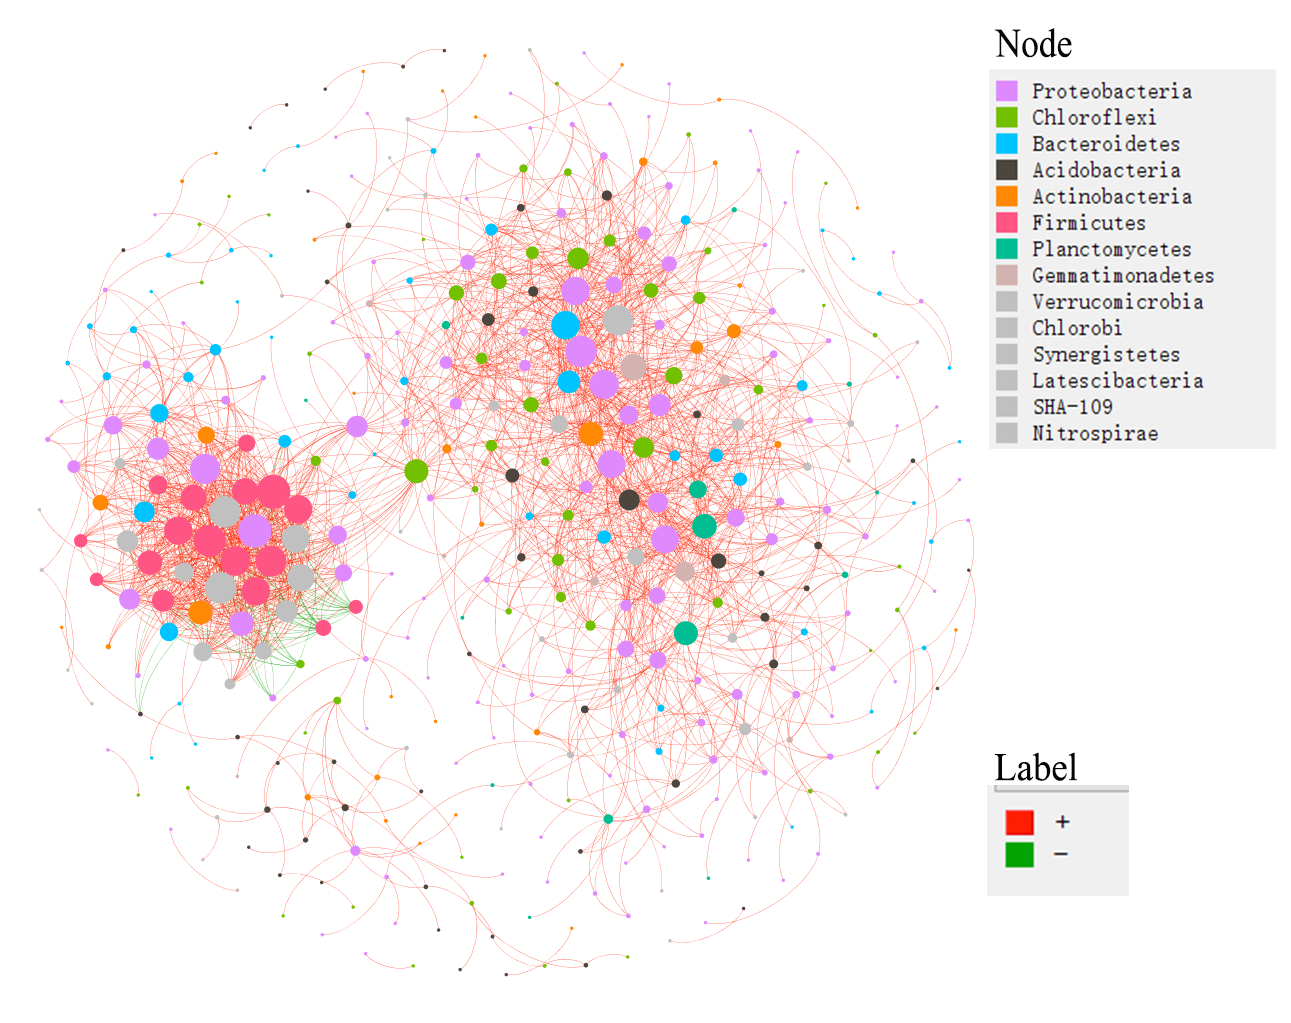
\includegraphics[width=550px]{Images/network2_spearman} \end{center}

\begin{Shaded}
\begin{Highlighting}[]
\CommentTok{\# calculate network attributes}
\NormalTok{t1}\SpecialCharTok{$}\FunctionTok{cal\_network\_attr}\NormalTok{()}
\CommentTok{\# return t1$res\_network\_attr}
\end{Highlighting}
\end{Shaded}

\begin{longtable}[]{@{}
  >{\centering\arraybackslash}p{(\columnwidth - 2\tabcolsep) * \real{0.35}}
  >{\centering\arraybackslash}p{(\columnwidth - 2\tabcolsep) * \real{0.14}}@{}}
\toprule
Property & Value \\
\midrule
\endhead
Vertex & 407 \\
Edge & 1989 \\
Average\_degree & 9.774 \\
Average\_path\_length & 3.878 \\
Network\_diameter & 9 \\
Clustering\_coefficient & 0.4698 \\
Density & 0.02407 \\
Heterogeneity & 1.194 \\
Centralization & 0.09908 \\
\bottomrule
\end{longtable}

\begin{Shaded}
\begin{Highlighting}[]
\CommentTok{\# classify the node; return t1$res\_node\_type}
\NormalTok{t1}\SpecialCharTok{$}\FunctionTok{cal\_node\_type}\NormalTok{()}
\CommentTok{\# return t1$res\_node\_type}
\CommentTok{\# we retain the file for the following example in trans\_func part}
\NormalTok{network\_node\_type }\OtherTok{\textless{}{-}}\NormalTok{ t1}\SpecialCharTok{$}\NormalTok{res\_node\_type}
\end{Highlighting}
\end{Shaded}

\begin{longtable}[]{@{}
  >{\centering\arraybackslash}p{(\columnwidth - 8\tabcolsep) * \real{0.22}}
  >{\centering\arraybackslash}p{(\columnwidth - 8\tabcolsep) * \real{0.15}}
  >{\centering\arraybackslash}p{(\columnwidth - 8\tabcolsep) * \real{0.12}}
  >{\centering\arraybackslash}p{(\columnwidth - 8\tabcolsep) * \real{0.12}}
  >{\centering\arraybackslash}p{(\columnwidth - 8\tabcolsep) * \real{0.26}}@{}}
\toprule
~ & z & module & p & taxa\_roles \\
\midrule
\endhead
\textbf{OTU\_50} & -1.305 & M2 & 0 & Peripheral nodes \\
\textbf{OTU\_1} & -0.04067 & M2 & 0 & Peripheral nodes \\
\textbf{OTU\_55} & -1.239 & M2 & 0 & Peripheral nodes \\
\textbf{OTU\_13824} & -0.2403 & M2 & 0 & Peripheral nodes \\
\textbf{OTU\_151} & -1.372 & M2 & 0.4444 & Peripheral nodes \\
\bottomrule
\end{longtable}

\begin{Shaded}
\begin{Highlighting}[]
\CommentTok{\# plot node roles in terms of the within{-}module connectivity and among{-}module connectivity}
\NormalTok{t1}\SpecialCharTok{$}\FunctionTok{plot\_taxa\_roles}\NormalTok{(}\AttributeTok{use\_type =} \DecValTok{1}\NormalTok{)}
\end{Highlighting}
\end{Shaded}

\begin{center}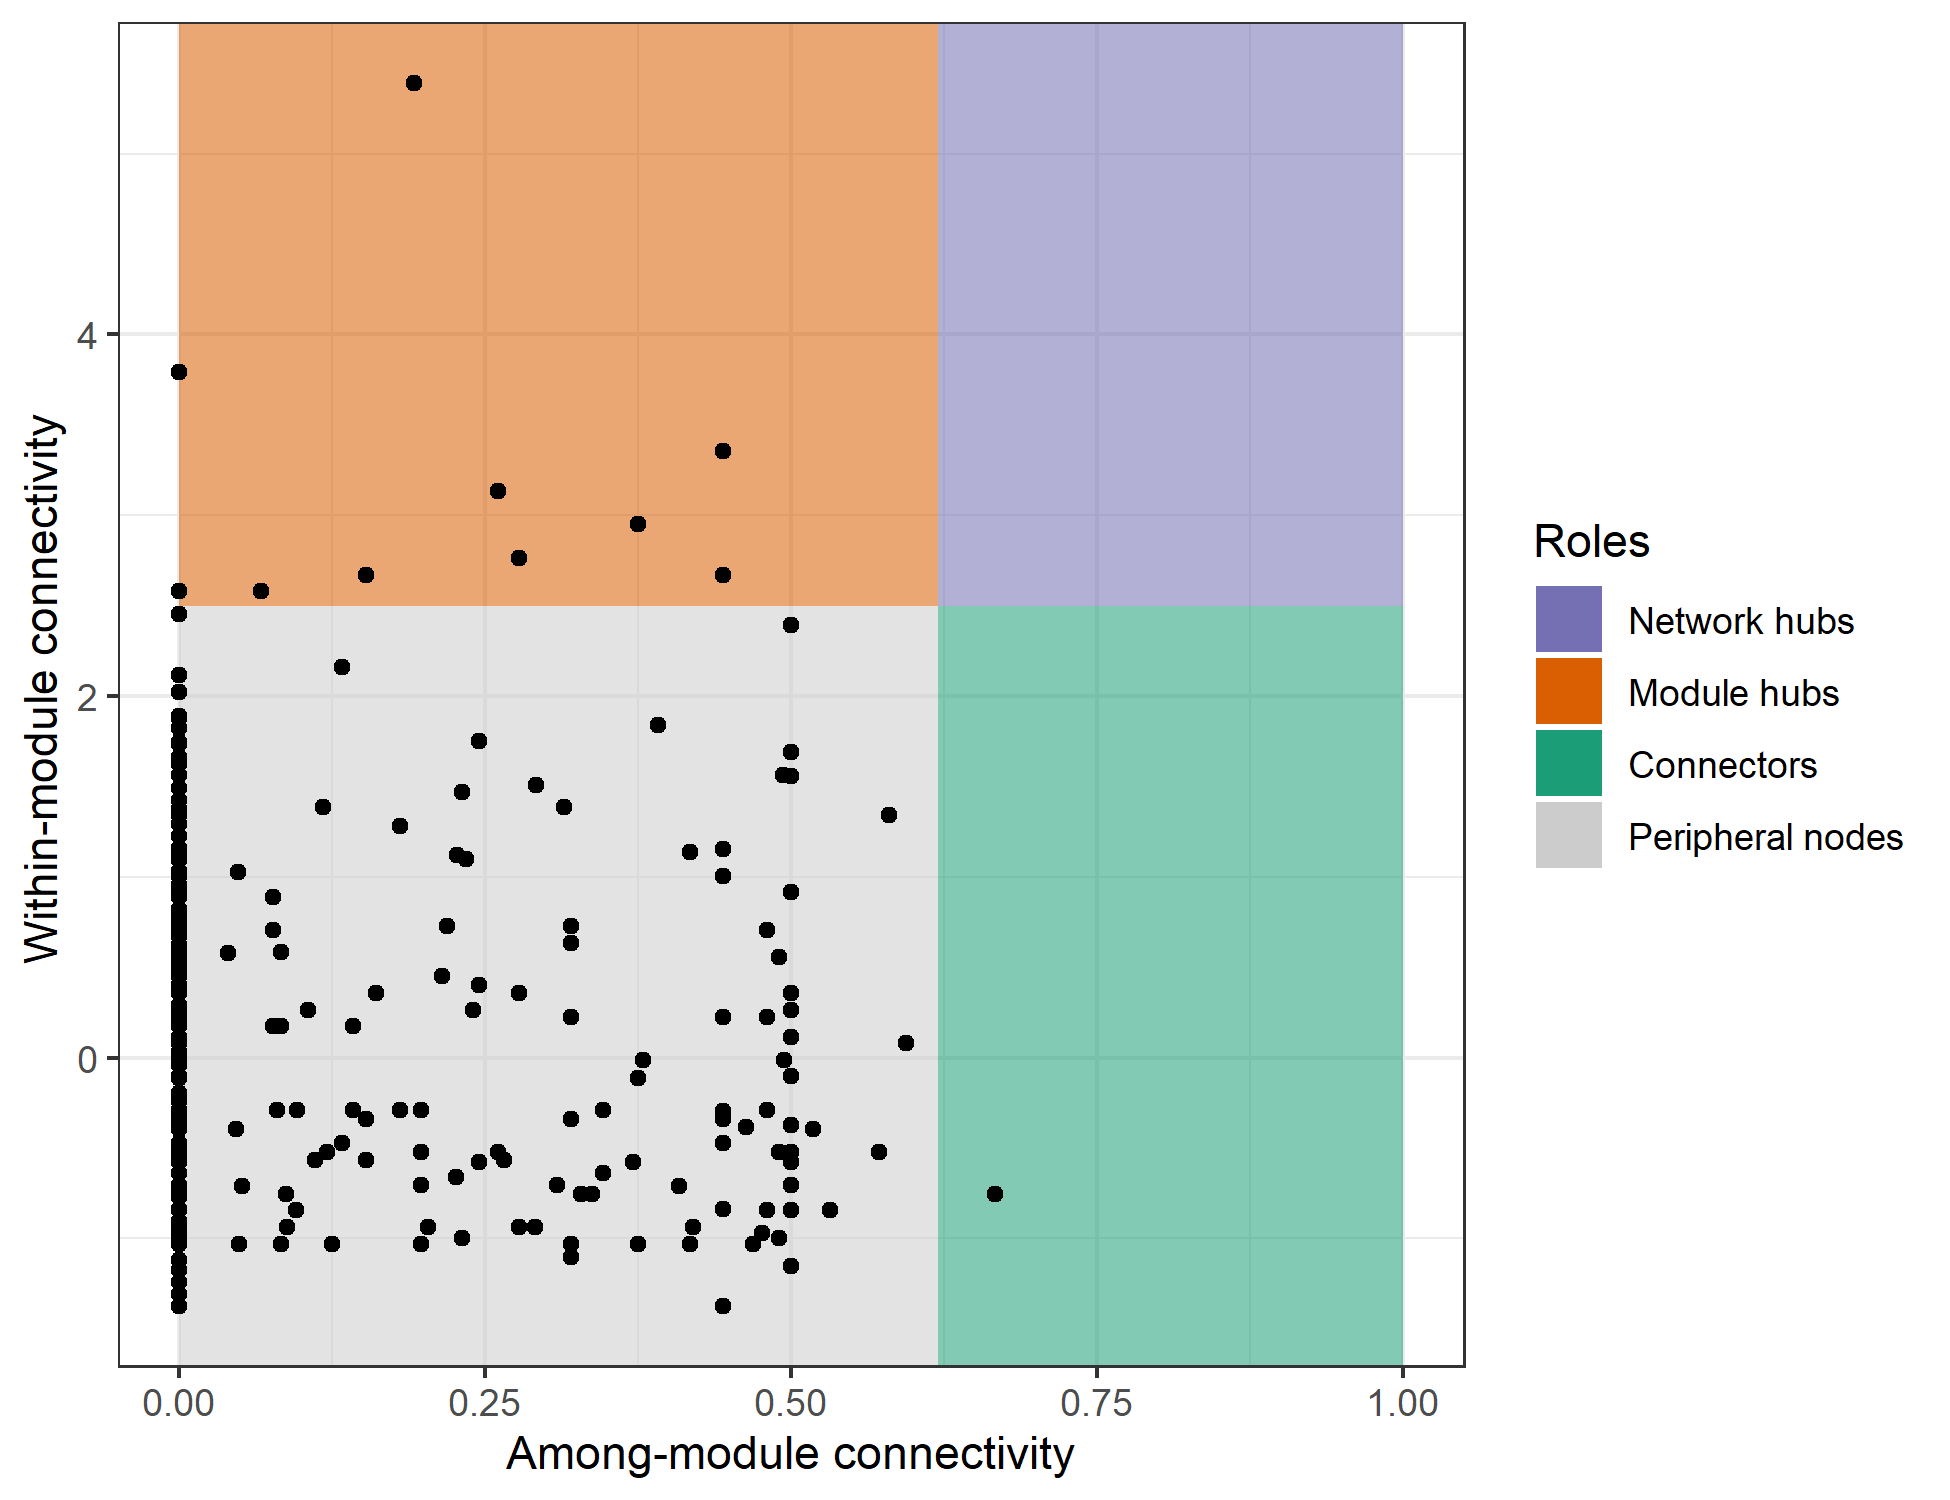
\includegraphics[width=700px]{Images/plot_taxa_roles} \end{center}

\begin{Shaded}
\begin{Highlighting}[]
\CommentTok{\# plot node roles with phylum information}
\NormalTok{t1}\SpecialCharTok{$}\FunctionTok{plot\_taxa\_roles}\NormalTok{(}\AttributeTok{use\_type =} \DecValTok{2}\NormalTok{)}
\end{Highlighting}
\end{Shaded}

\begin{center}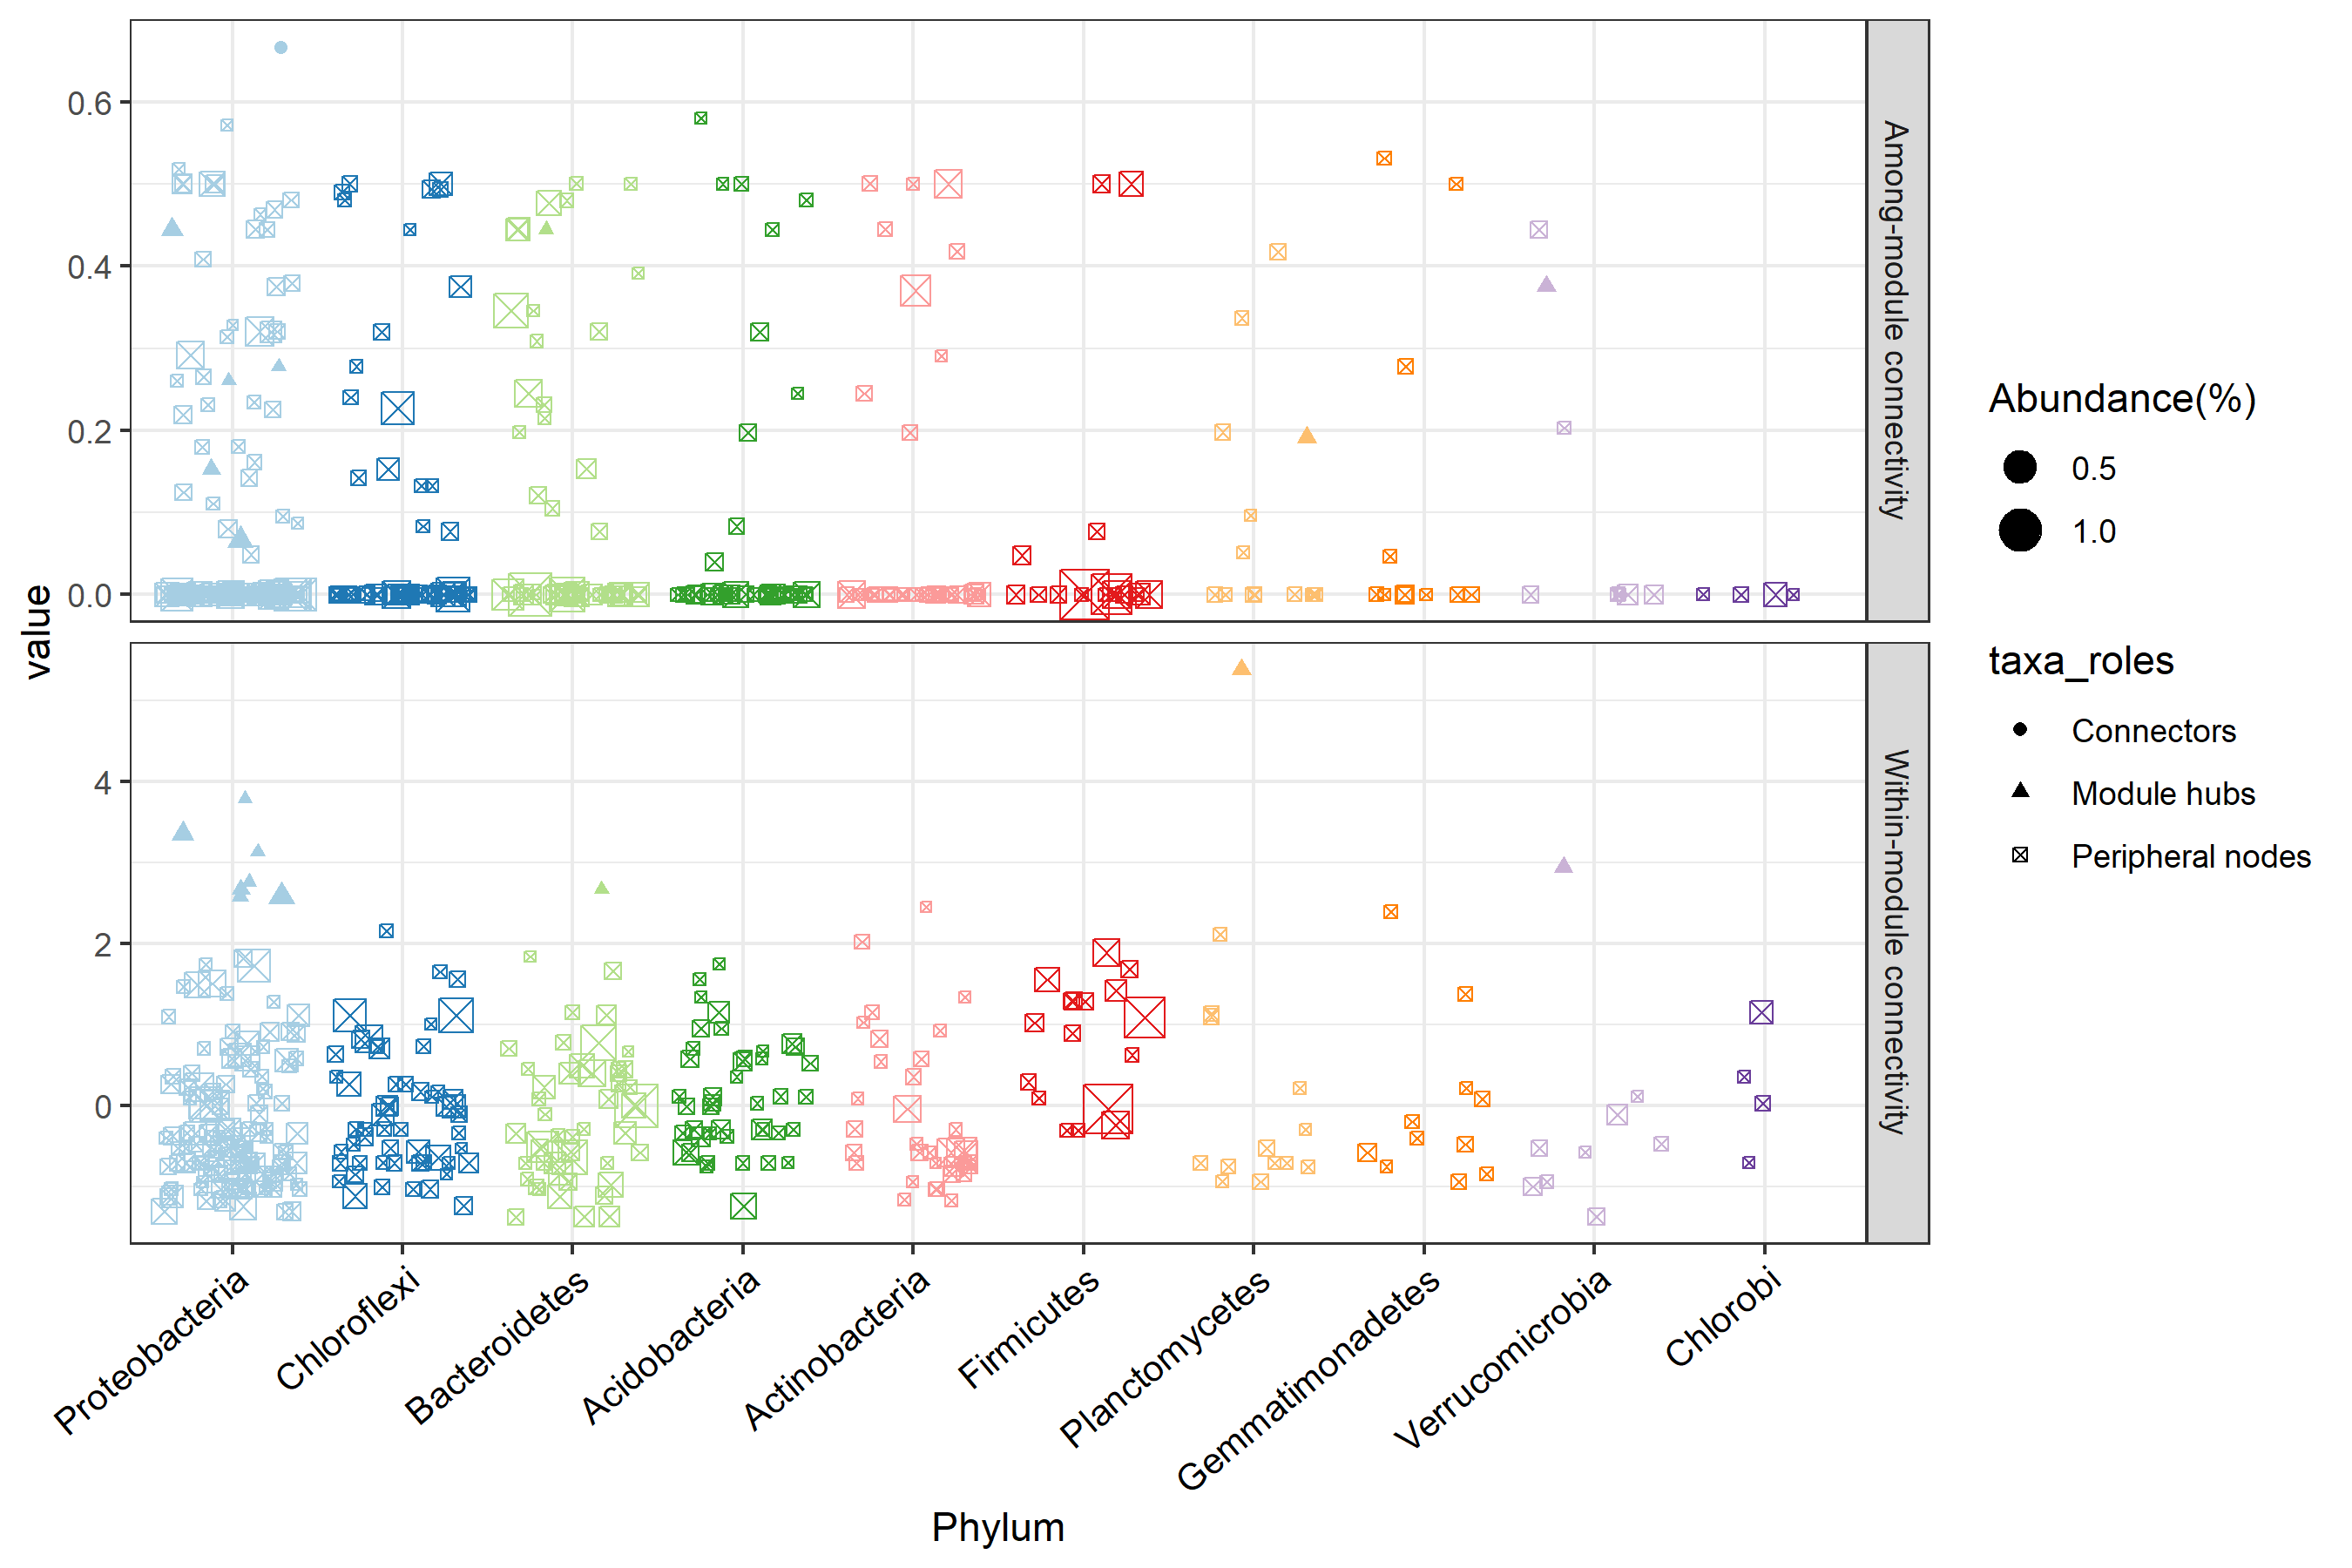
\includegraphics[width=800px]{Images/plot_taxa_roles_2} \end{center}

Now, we show the eigengene analysis of modules.
The eigengene of a module, i.e.~the first principal component of PCA, represents the main variance of the abundance in the species of the module.

\begin{Shaded}
\begin{Highlighting}[]
\NormalTok{t1}\SpecialCharTok{$}\FunctionTok{cal\_eigen}\NormalTok{()}
\CommentTok{\# return t1$res\_eigen}
\end{Highlighting}
\end{Shaded}

Then we perform correlation heatmap to show the relationships between eigengenes and environmental factors.

\begin{Shaded}
\begin{Highlighting}[]
\CommentTok{\# create trans\_env object like the above operation}
\NormalTok{t2 }\OtherTok{\textless{}{-}}\NormalTok{ trans\_env}\SpecialCharTok{$}\FunctionTok{new}\NormalTok{(}\AttributeTok{dataset =}\NormalTok{ dataset, }\AttributeTok{add\_data =}\NormalTok{ env\_data\_16S[, }\DecValTok{4}\SpecialCharTok{:}\DecValTok{11}\NormalTok{])}
\CommentTok{\# calculate correlations}
\NormalTok{t2}\SpecialCharTok{$}\FunctionTok{cal\_cor}\NormalTok{(}\AttributeTok{add\_abund\_table =}\NormalTok{ t1}\SpecialCharTok{$}\NormalTok{res\_eigen)}
\CommentTok{\# plot the correlation heatmap}
\NormalTok{t2}\SpecialCharTok{$}\FunctionTok{plot\_cor}\NormalTok{()}
\end{Highlighting}
\end{Shaded}

\begin{center}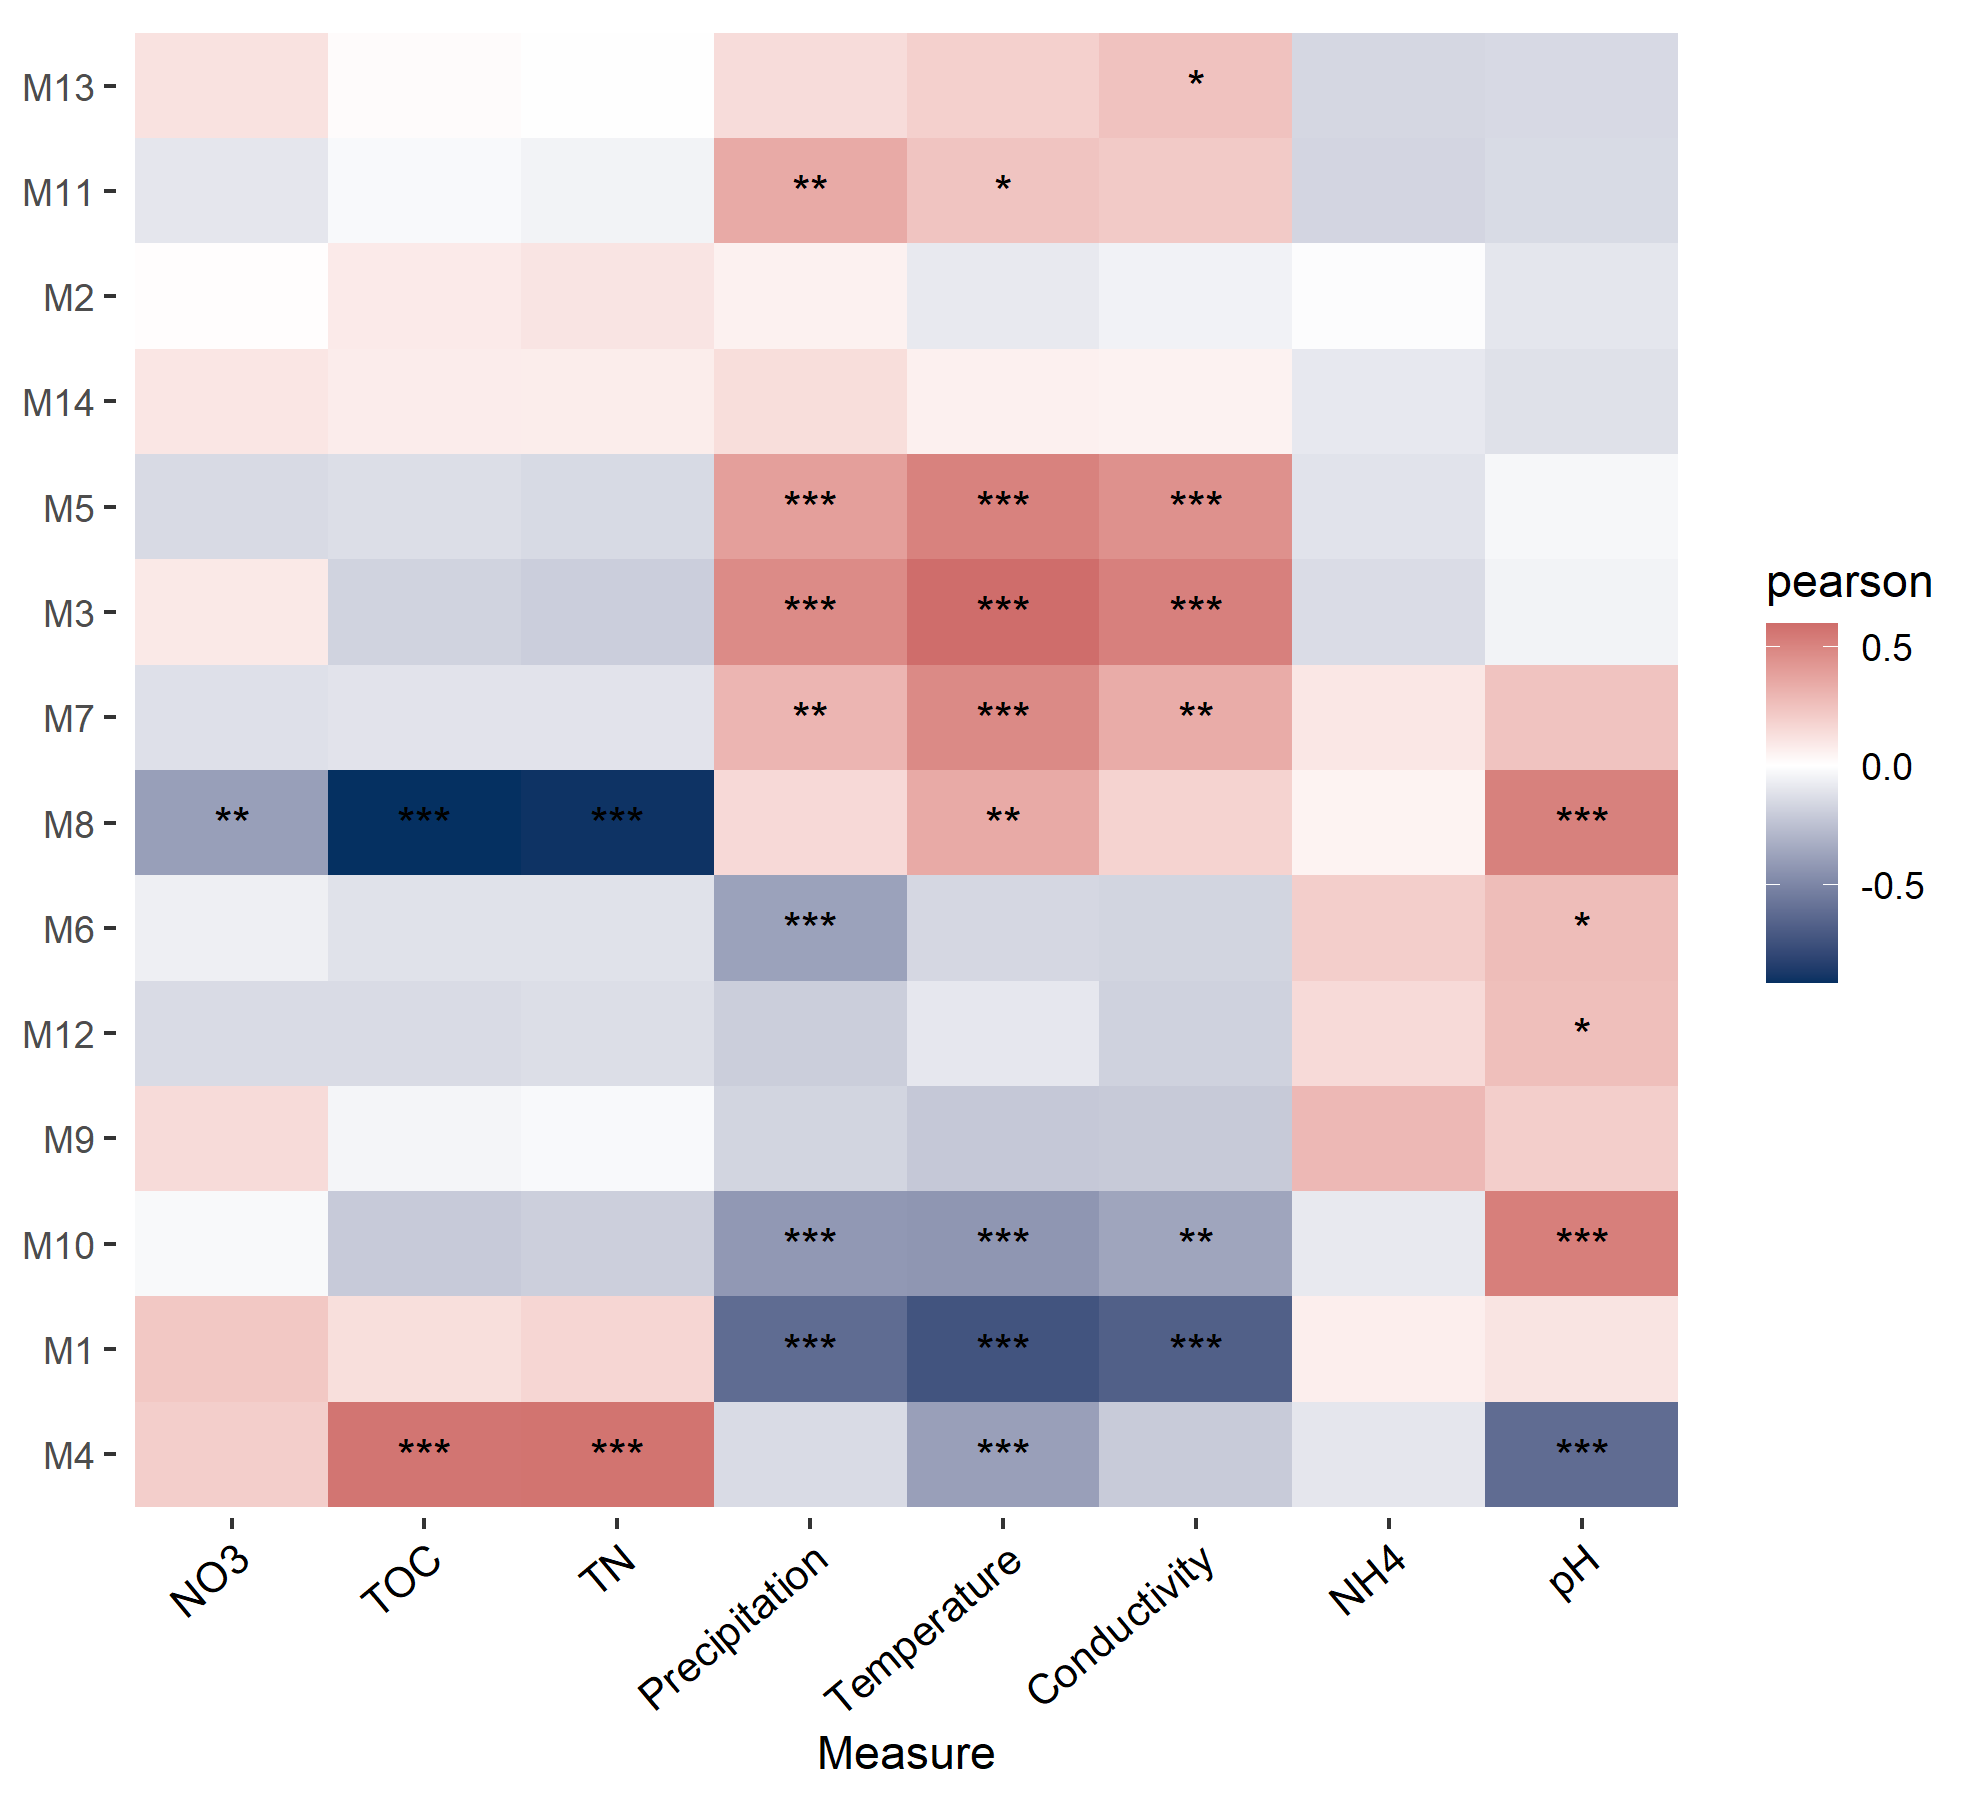
\includegraphics[width=600px]{Images/Env_module_eigen} \end{center}

The subset\_network() function can be used to extract a part of nodes and edges among these nodes from the network.
In this function, you should provide the nodes you need using the node parameter.

\begin{Shaded}
\begin{Highlighting}[]
\CommentTok{\# extract a sub network that contains all nodes in module M1}
\NormalTok{t1}\SpecialCharTok{$}\FunctionTok{subset\_network}\NormalTok{(}\AttributeTok{node =}\NormalTok{ t1}\SpecialCharTok{$}\NormalTok{res\_node\_type }\SpecialCharTok{\%\textgreater{}\%}\NormalTok{ .[.}\SpecialCharTok{$}\NormalTok{module }\SpecialCharTok{==} \StringTok{"M1"}\NormalTok{, ] }\SpecialCharTok{\%\textgreater{}\%}\NormalTok{ rownames, }\AttributeTok{rm\_single =} \ConstantTok{TRUE}\NormalTok{)}
\CommentTok{\# return a new network with igraph class}
\CommentTok{\# extract sub network in which all edge labels are "+", i.e. positive edges}
\NormalTok{t1}\SpecialCharTok{$}\FunctionTok{subset\_network}\NormalTok{(}\AttributeTok{edge =} \StringTok{"+"}\NormalTok{)}
\end{Highlighting}
\end{Shaded}

Then we show the next implemented network construction approach:
SPIEC-EASI (SParse InversE Covariance Estimation for Ecological Association Inference) network in SpiecEasi R package \citep{Kurtz_Sparse_2015}.

\begin{Shaded}
\begin{Highlighting}[]
\CommentTok{\# cal\_cor select NA}
\NormalTok{t1 }\OtherTok{\textless{}{-}}\NormalTok{ trans\_network}\SpecialCharTok{$}\FunctionTok{new}\NormalTok{(}\AttributeTok{dataset =}\NormalTok{ dataset, }\AttributeTok{cal\_cor =} \ConstantTok{NA}\NormalTok{, }\AttributeTok{taxa\_level =} \StringTok{"OTU"}\NormalTok{, }\AttributeTok{filter\_thres =} \FloatTok{0.0005}\NormalTok{)}
\CommentTok{\# require SpiecEasi package  https://github.com/zdk123/SpiecEasi}
\NormalTok{t1}\SpecialCharTok{$}\FunctionTok{cal\_network}\NormalTok{(}\AttributeTok{network\_method =} \StringTok{"SpiecEasi"}\NormalTok{)}
\CommentTok{\# see t1$res\_network}
\end{Highlighting}
\end{Shaded}

We also introduce the third network construction approach: Probabilistic Graphical Models (PGM), which is implemented in julia package FlashWeave\citep{Tackmann_Rapid_2019}.
It predicts ecological interactions among microbes from large-scale compositional abundance data (i.e.~OTU tables constructed from sequencing data)
through statistical co-occurrence.
If you want to use this method like the following code, you should first install julia language in your computer and the FlashWeave package,
and add the julia in the computer path.

\begin{enumerate}
\def\labelenumi{\arabic{enumi}.}
\tightlist
\item
  download and install julia from \url{https://julialang.org/downloads/}\\
\item
  Put julia in the computer env PATH, such as your\_directory\_path\Julia\bin  
\item
  Open terminal or cmd or Powershell, open julia, install FlashWeave following the operation in \url{https://github.com/meringlab/FlashWeave.jl}
\end{enumerate}

\begin{Shaded}
\begin{Highlighting}[]
\CommentTok{\# cal\_cor select NA}
\NormalTok{t1 }\OtherTok{\textless{}{-}}\NormalTok{ trans\_network}\SpecialCharTok{$}\FunctionTok{new}\NormalTok{(}\AttributeTok{dataset =}\NormalTok{ dataset, }\AttributeTok{cal\_cor =} \ConstantTok{NA}\NormalTok{, }\AttributeTok{taxa\_level =} \StringTok{"OTU"}\NormalTok{, }\AttributeTok{filter\_thres =} \FloatTok{0.0001}\NormalTok{)}
\CommentTok{\# require Julia in the computer path, and the package FlashWeave}
\NormalTok{t1}\SpecialCharTok{$}\FunctionTok{cal\_network}\NormalTok{(}\AttributeTok{network\_method =} \StringTok{"PGM"}\NormalTok{)}
\CommentTok{\# see t1$res\_network}
\end{Highlighting}
\end{Shaded}

\hypertarget{trans_func-class}{%
\section{trans\_func class}\label{trans_func-class}}

 Ecological researchers are usually interested in the the funtional profiles of microbial communities,
because functional or metabolic data is powerful to explain the structure and dynamics of microbial communities and to infer the underlying mechanisms.
As metagenomic sequencing is complicated and expensive, using amplicon sequencing data to predict functional profiles is a good choice.
Several software are often used for this goal, such as PICRUSt\citep{Langille_Predictive_2013}, Tax4Fun\citep{Aßhauer_Tax4Fun_2015} and FAPROTAX\citep{Louca_High_2016, Louca_Decoupling_2016}.
These tools are great to be used for the prediction of functional profiles based on the prokaryotic communities from sequencing results.
In addition, it is also important to obtain the functions for each taxa or OTU, not just the whole profile of communities.
But it is hard to know exact functions of each OTU.
FAPROTAX database is a collection of the traits and characteristics of prokaryotes based on the known research results published in books and literatures.
We match the taxonomic information of prokaryotes against this database to identify the traits of prokaryotes on biogeochemical roles.
The NJC19 database\citep{Lim_Large_2020} is also available for animal associated prokaryotic data, such as human gut microbiota.
We also implement the FUNGuild \citep{Nguyen_FUNGuild_2016} and FungalTraits \citep{Polme_FungalTraits_2020} databases to identify the fungal traits.

\begin{Shaded}
\begin{Highlighting}[]
\CommentTok{\# Identify microbial traits}
\CommentTok{\# create object of trans\_func}
\NormalTok{t2 }\OtherTok{\textless{}{-}}\NormalTok{ trans\_func}\SpecialCharTok{$}\FunctionTok{new}\NormalTok{(dataset)}
\CommentTok{\# mapping the taxonomy to the database}
\CommentTok{\# this can recognize prokaryotes or fungi automatically.}
\CommentTok{\# default database for prokaryotes is FAPROTAX database}
\NormalTok{t2}\SpecialCharTok{$}\FunctionTok{cal\_spe\_func}\NormalTok{()}
\end{Highlighting}
\end{Shaded}

\begin{verbatim}
## Please also cite the original FAPROTAX paper: Louca et al. (2016).
\end{verbatim}

\begin{verbatim}
## Decoupling function and taxonomy in the global ocean microbiome. Science, 353(6305), 1272.
\end{verbatim}

\begin{verbatim}
## The functional table is stored in object$res_spe_func ...
\end{verbatim}

\begin{Shaded}
\begin{Highlighting}[]
\CommentTok{\# return t2$res\_spe\_func, 1 represent function exists, 0 represent no or cannot confirmed.}
\end{Highlighting}
\end{Shaded}

\begin{Shaded}
\begin{Highlighting}[]
\NormalTok{t2}\SpecialCharTok{$}\NormalTok{res\_spe\_func[}\DecValTok{1}\SpecialCharTok{:}\DecValTok{5}\NormalTok{, }\DecValTok{1}\SpecialCharTok{:}\DecValTok{2}\NormalTok{]}
\end{Highlighting}
\end{Shaded}

\begin{longtable}[]{@{}
  >{\centering\arraybackslash}p{(\columnwidth - 4\tabcolsep) * \real{0.21}}
  >{\centering\arraybackslash}p{(\columnwidth - 4\tabcolsep) * \real{0.22}}
  >{\centering\arraybackslash}p{(\columnwidth - 4\tabcolsep) * \real{0.42}}@{}}
\toprule
~ & methanotrophy & acetoclastic\_methanogenesis \\
\midrule
\endhead
\textbf{OTU\_4272} & 0 & 0 \\
\textbf{OTU\_236} & 0 & 0 \\
\textbf{OTU\_399} & 0 & 0 \\
\textbf{OTU\_1556} & 0 & 0 \\
\textbf{OTU\_32} & 0 & 0 \\
\bottomrule
\end{longtable}

The percentages of the OTUs having the same trait can reflect the functional redundancy of this function in the community or the module in the network.

\begin{Shaded}
\begin{Highlighting}[]
\CommentTok{\# calculate the percentages of OTUs for each trait in each module of network}
\CommentTok{\# use\_community = FALSE represent calculating module, not community, node\_type\_table provide the module information}
\NormalTok{t2}\SpecialCharTok{$}\FunctionTok{cal\_spe\_func\_perc}\NormalTok{(}\AttributeTok{use\_community =} \ConstantTok{FALSE}\NormalTok{, }\AttributeTok{node\_type\_table =}\NormalTok{ network\_node\_type)}
\CommentTok{\# return t2$res\_spe\_func\_perc}
\CommentTok{\# we only plot some important traits, so we use the default group list to filter and show the traits.}
\NormalTok{t2}\SpecialCharTok{$}\FunctionTok{plot\_spe\_func\_perc}\NormalTok{(}\AttributeTok{select\_samples =} \FunctionTok{paste0}\NormalTok{(}\StringTok{"M"}\NormalTok{, }\DecValTok{1}\SpecialCharTok{:}\DecValTok{10}\NormalTok{))}
\CommentTok{\# M represents module, ordered by the nodes number from high to low}
\end{Highlighting}
\end{Shaded}

\begin{center}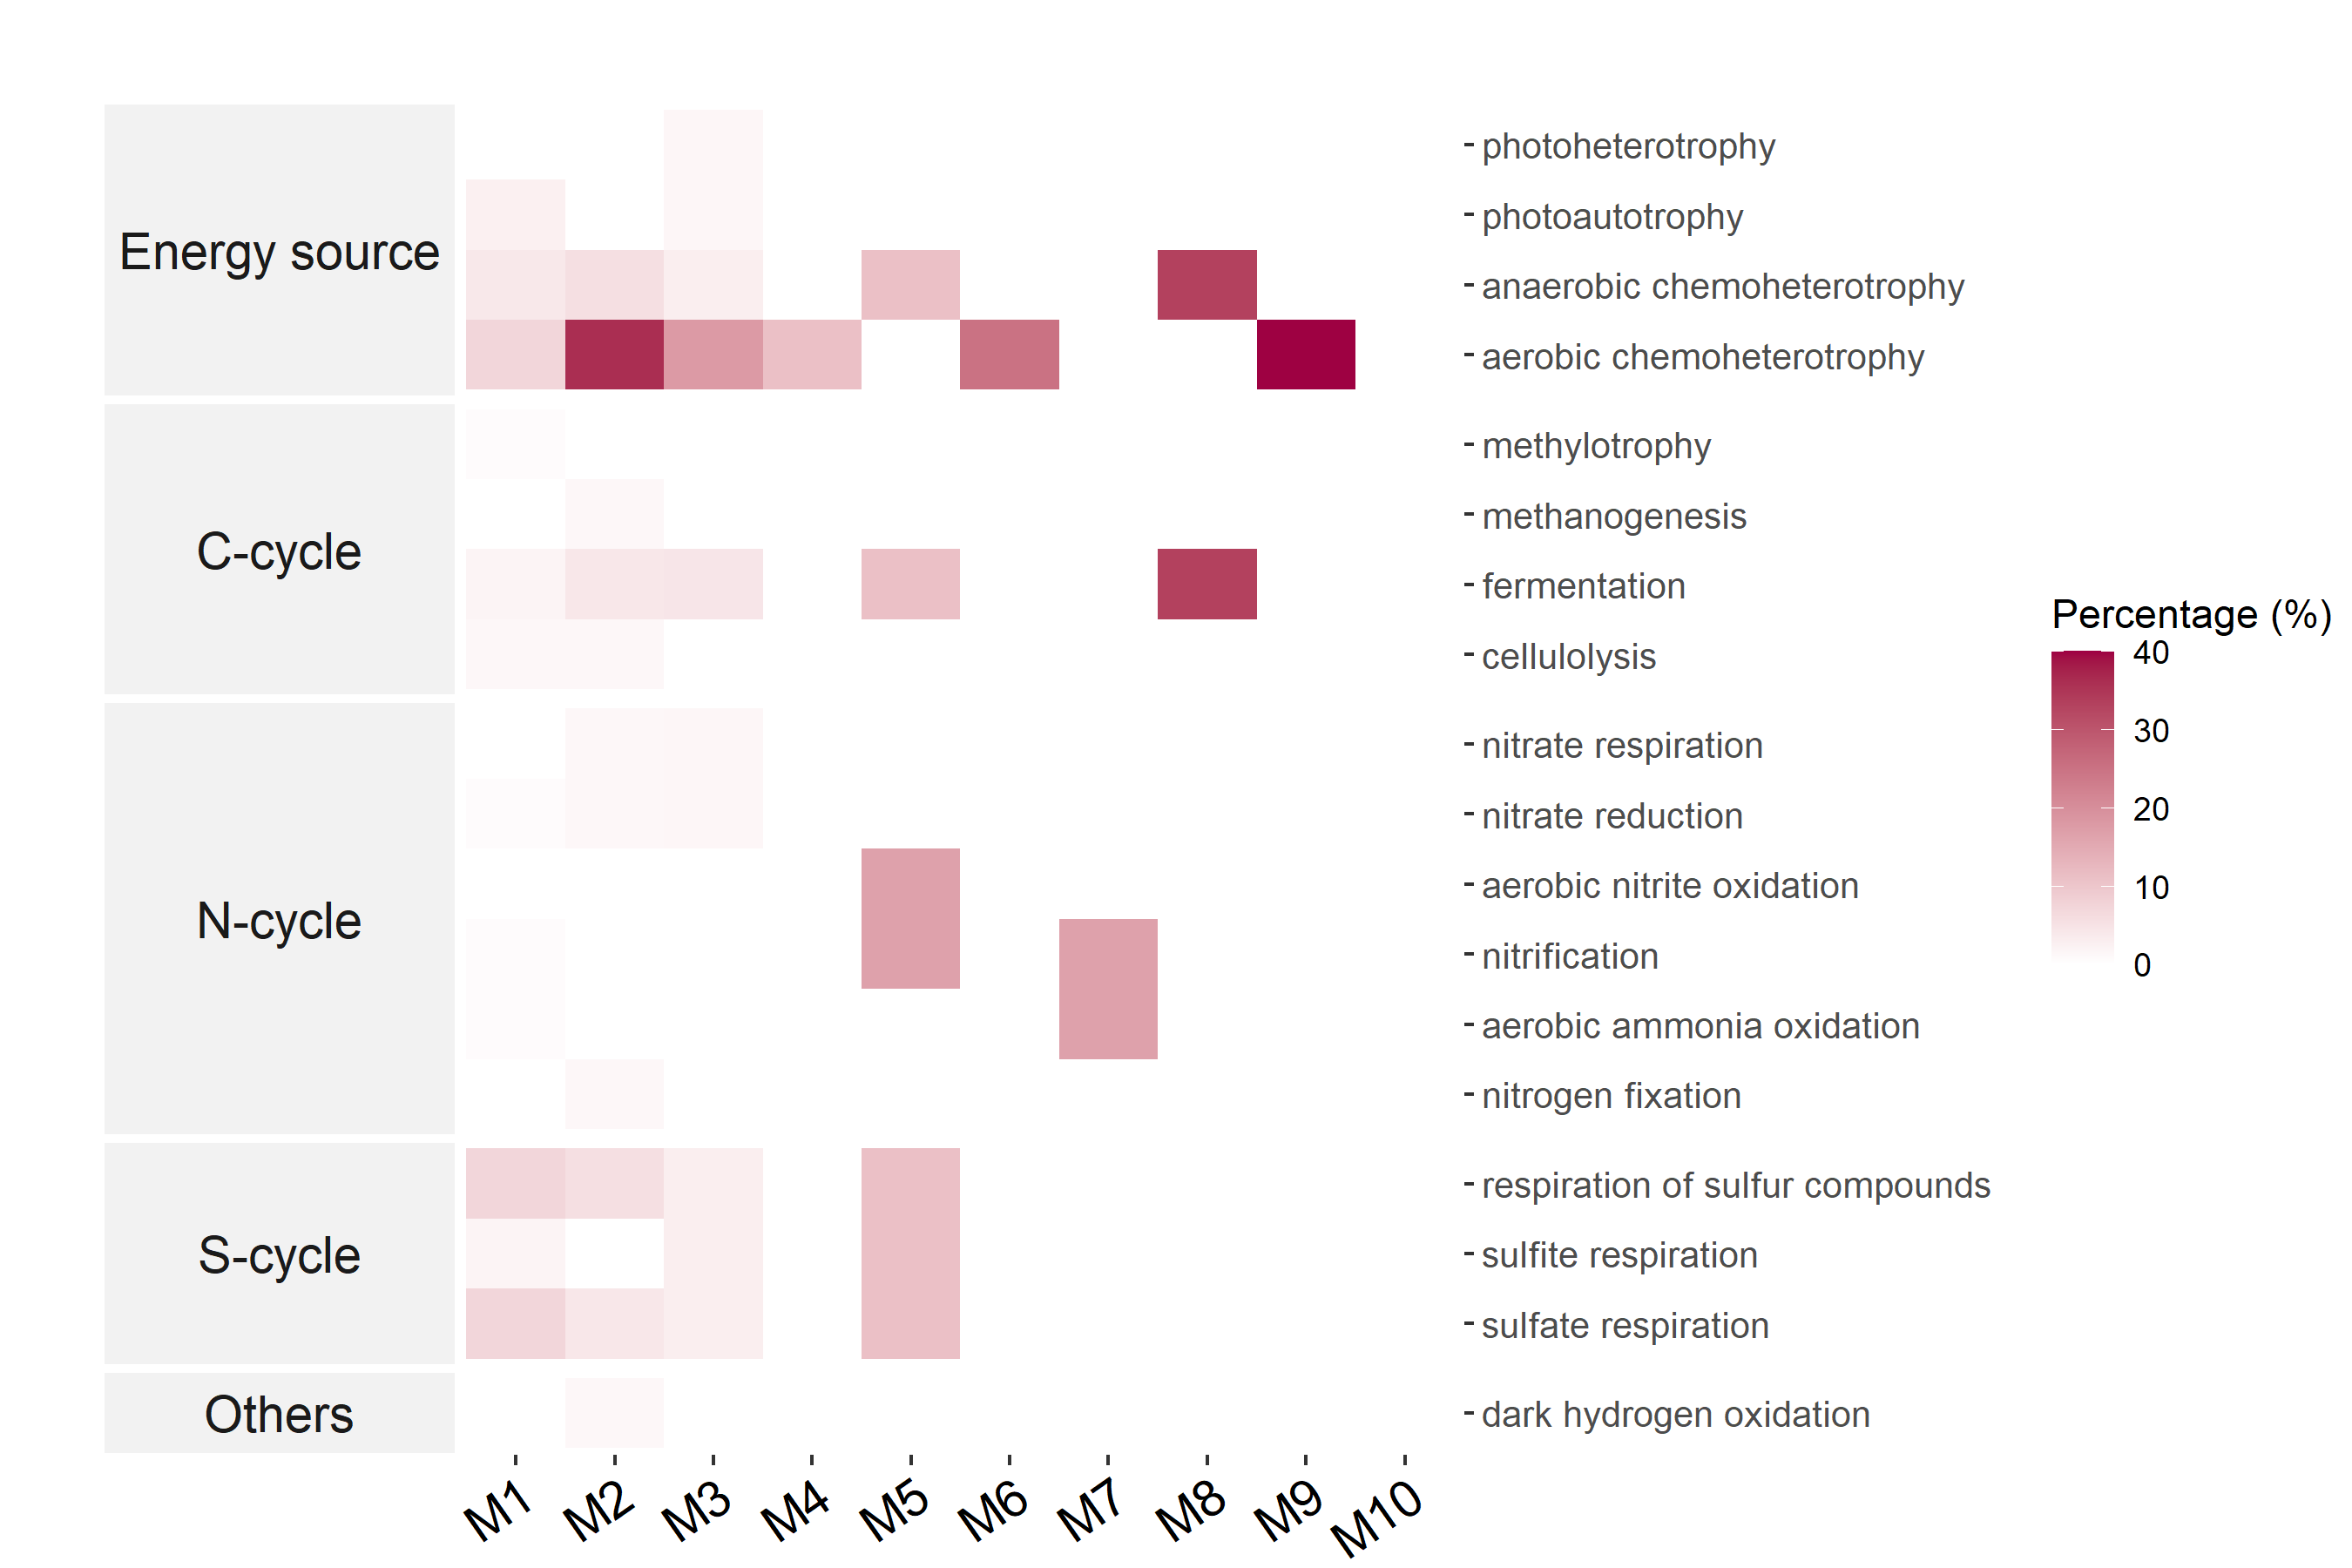
\includegraphics[width=700px]{Images/plot_func_perc} \end{center}

\begin{Shaded}
\begin{Highlighting}[]
\CommentTok{\# If you want to change the group list, reset the list t2$func\_group\_list}
\NormalTok{t2}\SpecialCharTok{$}\NormalTok{func\_group\_list}
\CommentTok{\# use show\_prok\_func to see the detailed information of prokaryotic traits}
\NormalTok{t2}\SpecialCharTok{$}\FunctionTok{show\_prok\_func}\NormalTok{(}\StringTok{"methanotrophy"}\NormalTok{)}
\end{Highlighting}
\end{Shaded}

\begin{Shaded}
\begin{Highlighting}[]
\CommentTok{\# calculate the percentages for communities}
\NormalTok{t2}\SpecialCharTok{$}\FunctionTok{cal\_spe\_func\_perc}\NormalTok{(}\AttributeTok{use\_community =} \ConstantTok{TRUE}\NormalTok{)}
\end{Highlighting}
\end{Shaded}

\begin{verbatim}
## The result table is stored in object$res_spe_func_perc ...
\end{verbatim}

\begin{Shaded}
\begin{Highlighting}[]
\CommentTok{\# t2$res\_spe\_func\_perc[1:5, 1:2]}
\end{Highlighting}
\end{Shaded}

\begin{longtable}[]{@{}
  >{\centering\arraybackslash}p{(\columnwidth - 4\tabcolsep) * \real{0.12}}
  >{\centering\arraybackslash}p{(\columnwidth - 4\tabcolsep) * \real{0.22}}
  >{\centering\arraybackslash}p{(\columnwidth - 4\tabcolsep) * \real{0.42}}@{}}
\toprule
~ & methanotrophy & acetoclastic\_methanogenesis \\
\midrule
\endhead
\textbf{S1} & 0.39 & 0.04 \\
\textbf{S2} & 0.27 & 0 \\
\textbf{S3} & 0.48 & 0 \\
\textbf{S4} & 0.48 & 0 \\
\textbf{S5} & 0.56 & 0 \\
\bottomrule
\end{longtable}

\begin{Shaded}
\begin{Highlighting}[]
\CommentTok{\# then we try to correlate the res\_spe\_func\_perc of communities to environmental variables}
\NormalTok{t3 }\OtherTok{\textless{}{-}}\NormalTok{ trans\_env}\SpecialCharTok{$}\FunctionTok{new}\NormalTok{(}\AttributeTok{dataset =}\NormalTok{ dataset, }\AttributeTok{add\_data =}\NormalTok{ env\_data\_16S[, }\DecValTok{4}\SpecialCharTok{:}\DecValTok{11}\NormalTok{])}
\NormalTok{t3}\SpecialCharTok{$}\FunctionTok{cal\_cor}\NormalTok{(}\AttributeTok{add\_abund\_table =}\NormalTok{ t2}\SpecialCharTok{$}\NormalTok{res\_spe\_func\_perc, }\AttributeTok{cor\_method =} \StringTok{"spearman"}\NormalTok{)}
\NormalTok{t3}\SpecialCharTok{$}\FunctionTok{plot\_cor}\NormalTok{(}\AttributeTok{pheatmap =} \ConstantTok{TRUE}\NormalTok{)}
\end{Highlighting}
\end{Shaded}

\begin{center}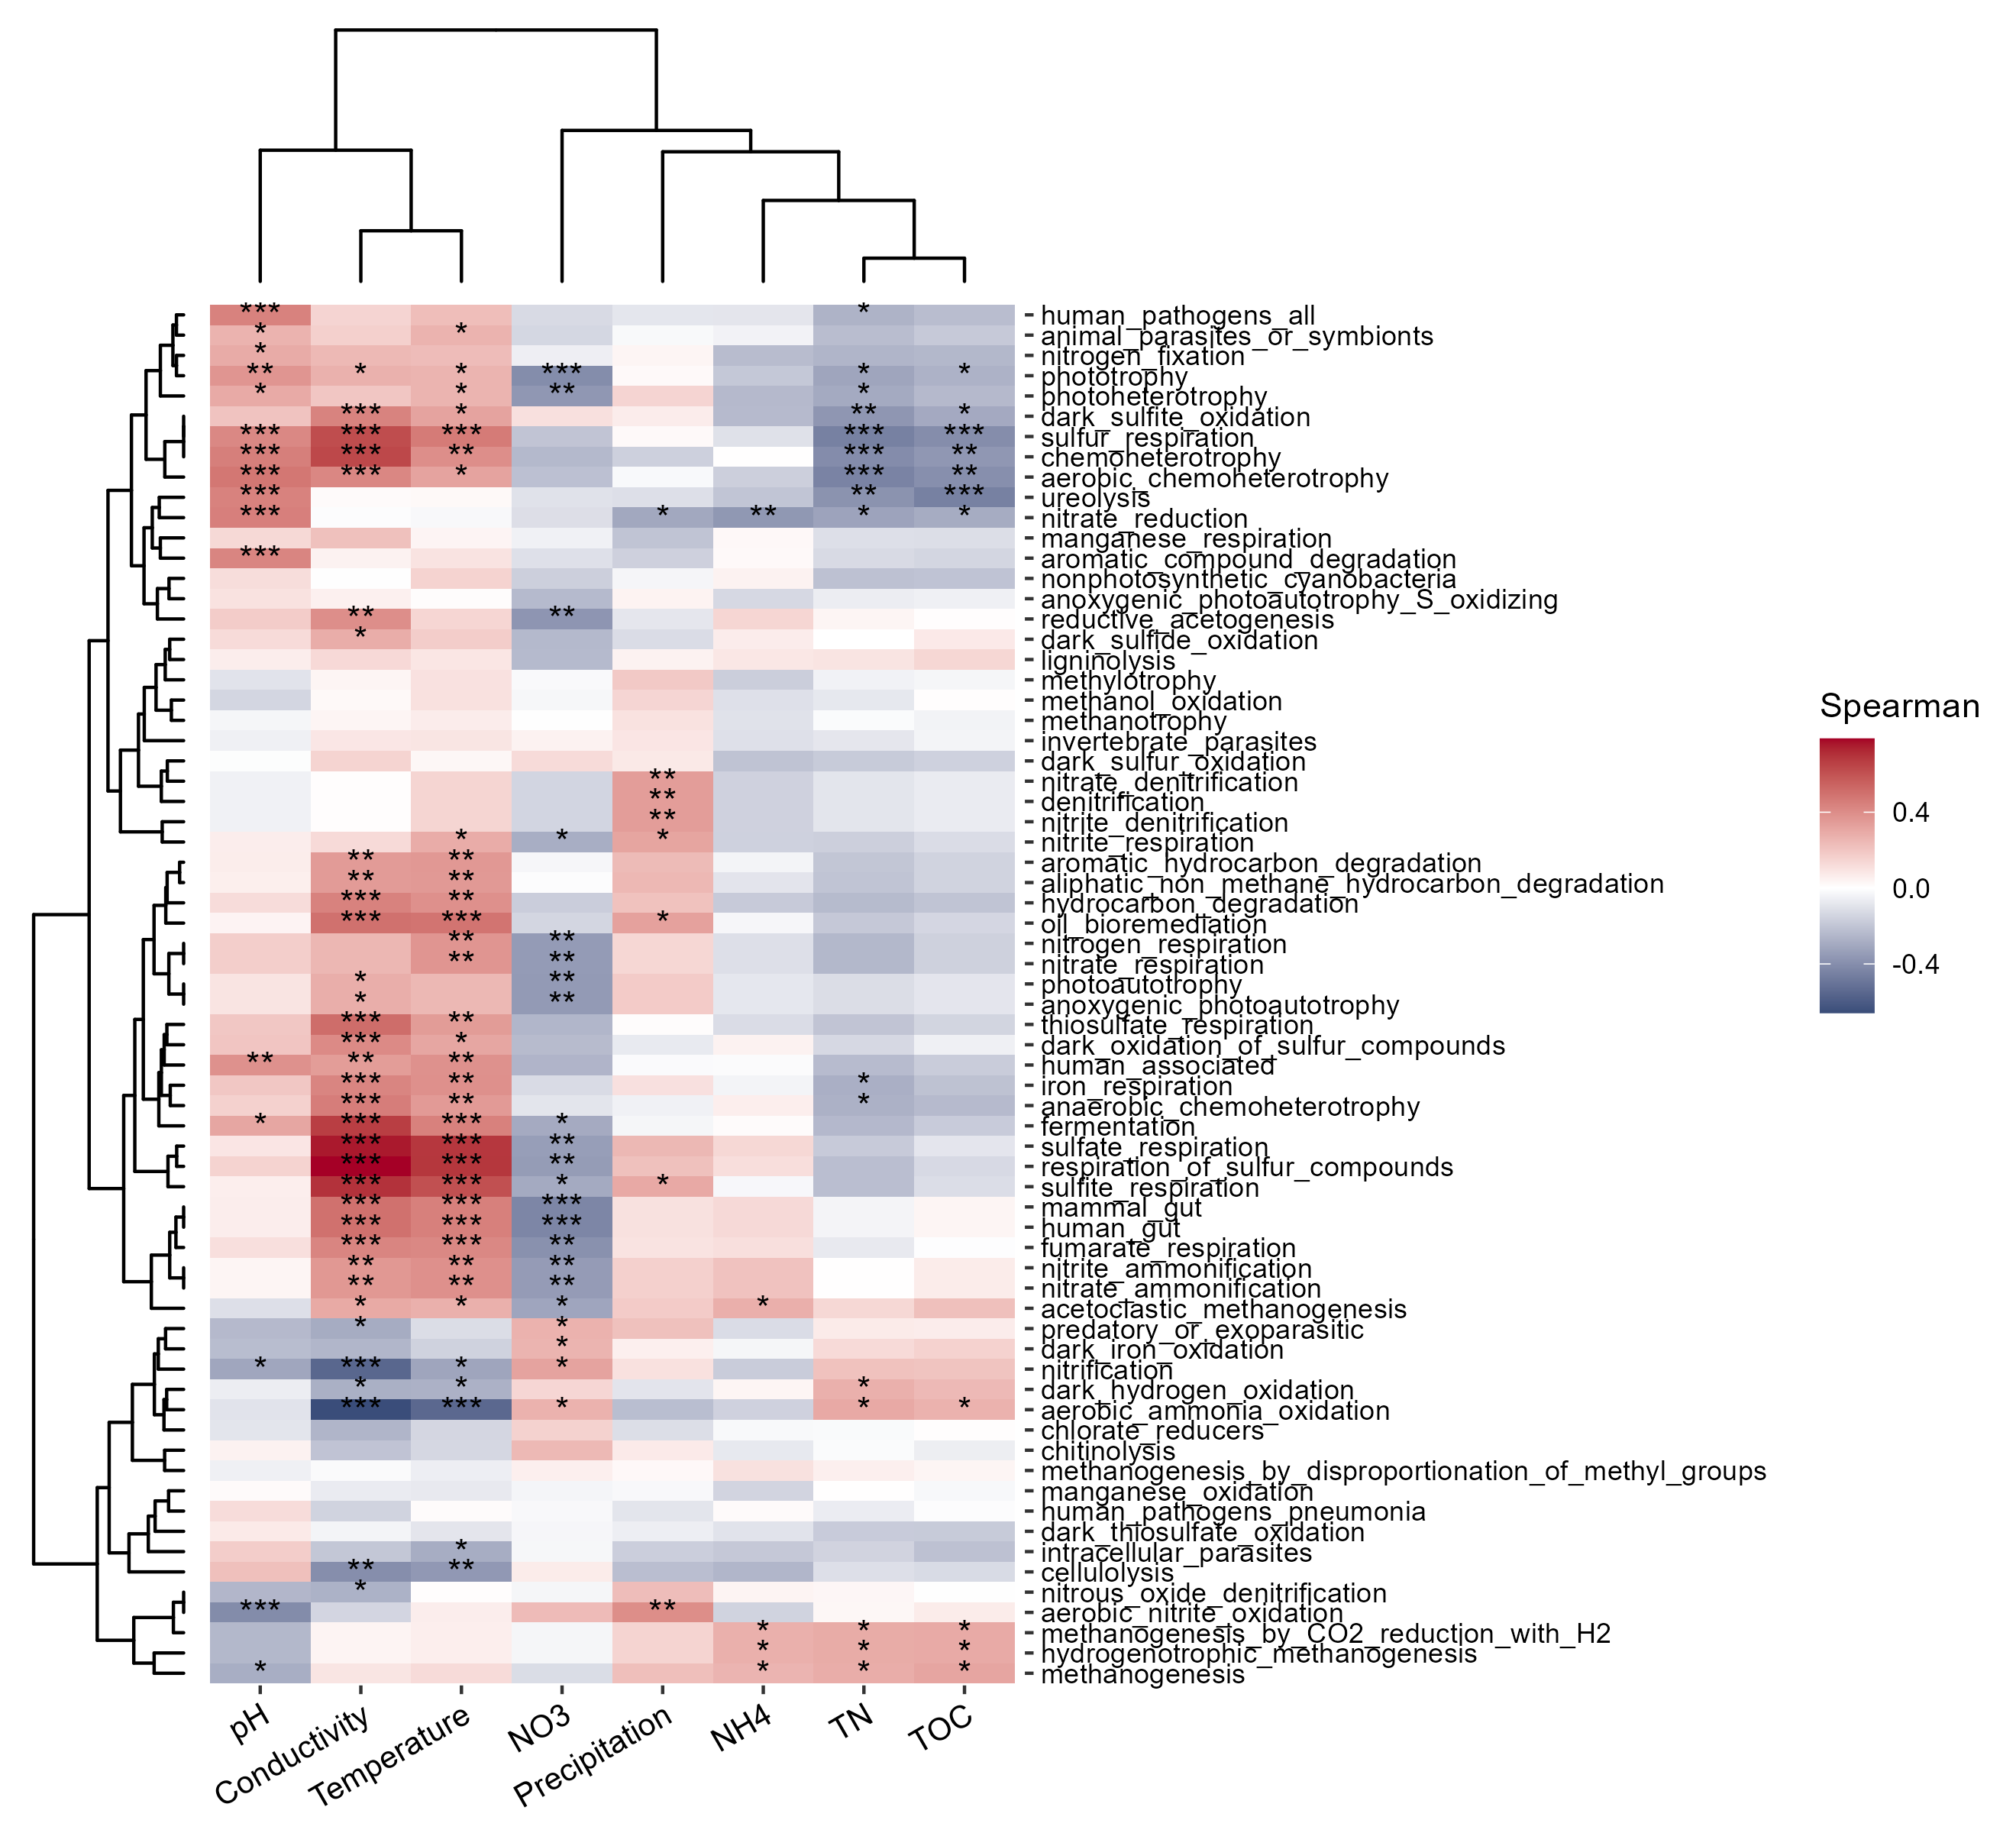
\includegraphics[width=800px]{Images/plot_func_perc_corr} \end{center}

Tax4Fun requires a strict input file demand on the taxonomic information.
To analyze the trimmed or changed OTU data in R with Tax4Fun, we provide a link to the Tax4Fun functional prediction.

\begin{Shaded}
\begin{Highlighting}[]
\NormalTok{t1 }\OtherTok{\textless{}{-}}\NormalTok{ trans\_func}\SpecialCharTok{$}\FunctionTok{new}\NormalTok{(dataset)}
\CommentTok{\# install Tax4Fun package and download SILVA123 ref data from  http://tax4fun.gobics.de/}
\CommentTok{\# decompress SILVA123; provide path in folderReferenceData as you put}
\NormalTok{t1}\SpecialCharTok{$}\FunctionTok{cal\_tax4fun}\NormalTok{(}\AttributeTok{folderReferenceData =} \StringTok{"./SILVA123"}\NormalTok{)}
\end{Highlighting}
\end{Shaded}

\begin{verbatim}
## 载入需要的程辑包:Tax4Fun
\end{verbatim}

\begin{verbatim}
## 载入需要的程辑包:Matrix
\end{verbatim}

\begin{verbatim}
## 载入需要的程辑包:qiimer
\end{verbatim}

\begin{verbatim}
## 载入需要的程辑包:biom
\end{verbatim}

\begin{verbatim}
## Warning in write.table(otu_file, file = output, append = TRUE, quote = FALSE, :
## appending column names to file
\end{verbatim}

\begin{verbatim}
## The KO abundance result is stored in object$tax4fun_KO ...
\end{verbatim}

\begin{verbatim}
## The pathway abundance result is stored in object$tax4fun_path ...
\end{verbatim}

\begin{Shaded}
\begin{Highlighting}[]
\CommentTok{\# return two files: t1$tax4fun\_KO: KO file; t1$tax4fun\_path: pathway file.}
\CommentTok{\# t1$tax4fun\_KO$Tax4FunProfile[1:5, 1:2]}
\end{Highlighting}
\end{Shaded}

\begin{longtable}[]{@{}
  >{\centering\arraybackslash}p{(\columnwidth - 4\tabcolsep) * \real{0.12}}
  >{\centering\arraybackslash}p{(\columnwidth - 4\tabcolsep) * \real{0.44}}
  >{\centering\arraybackslash}p{(\columnwidth - 4\tabcolsep) * \real{0.44}}@{}}
\toprule
~ & K00001; alcohol dehydrogenase
{[}EC:1.1.1.1{]} & K00002; alcohol dehydrogenase
(NADP+) {[}EC:1.1.1.2{]} \\
\midrule
\endhead
\textbf{S1} & 0.0004823 & 5.942e-06 \\
\textbf{S2} & 0.0005266 & 4.017e-06 \\
\textbf{S3} & 0.0005054 & 6.168e-06 \\
\textbf{S4} & 0.0005109 & 5.888e-06 \\
\textbf{S5} & 0.0005083 & 5.547e-06 \\
\bottomrule
\end{longtable}

Now, we use pathway file to analyze the abundance of pathway.

\begin{Shaded}
\begin{Highlighting}[]
\CommentTok{\# must transpose to taxa row, sample column}
\NormalTok{pathway\_file }\OtherTok{\textless{}{-}}\NormalTok{ t1}\SpecialCharTok{$}\NormalTok{tax4fun\_path}\SpecialCharTok{$}\NormalTok{Tax4FunProfile }\SpecialCharTok{\%\textgreater{}\%}\NormalTok{ t }\SpecialCharTok{\%\textgreater{}\%}\NormalTok{ as.data.frame}
\CommentTok{\# filter rownames, only keep ko+number}
\FunctionTok{rownames}\NormalTok{(pathway\_file) }\SpecialCharTok{\%\textless{}\textgreater{}\%} \FunctionTok{gsub}\NormalTok{(}\StringTok{"(\^{}.*);}\SpecialCharTok{\textbackslash{}\textbackslash{}}\StringTok{s.*"}\NormalTok{, }\StringTok{"}\SpecialCharTok{\textbackslash{}\textbackslash{}}\StringTok{1"}\NormalTok{, .)}
\CommentTok{\# load the pathway hierarchical metadata}
\FunctionTok{data}\NormalTok{(ko\_map)}
\CommentTok{\# create a microtable object, familiar?}
\NormalTok{func1 }\OtherTok{\textless{}{-}}\NormalTok{ microtable}\SpecialCharTok{$}\FunctionTok{new}\NormalTok{(}\AttributeTok{otu\_table =}\NormalTok{ pathway\_file, }\AttributeTok{tax\_table =}\NormalTok{ ko\_map, }\AttributeTok{sample\_table =}\NormalTok{ t1}\SpecialCharTok{$}\NormalTok{sample\_table)}
\FunctionTok{print}\NormalTok{(func1)}
\end{Highlighting}
\end{Shaded}

\begin{verbatim}
## microtable class:
## sample_table have 90 rows and 4 columns
## otu_table have 284 rows and 90 columns
## tax_table have 341 rows and 3 columns
\end{verbatim}

Now, we need to trim data and calculate abundance.

\begin{Shaded}
\begin{Highlighting}[]
\NormalTok{func1}\SpecialCharTok{$}\FunctionTok{tidy\_dataset}\NormalTok{()}
\CommentTok{\# calculate abundance automatically at three levels: level\_1, level\_2, level\_3}
\NormalTok{func1}\SpecialCharTok{$}\FunctionTok{cal\_abund}\NormalTok{()}
\end{Highlighting}
\end{Shaded}

\begin{verbatim}
## The result is stored in object$taxa_abund ...
\end{verbatim}

\begin{Shaded}
\begin{Highlighting}[]
\FunctionTok{print}\NormalTok{(func1)}
\end{Highlighting}
\end{Shaded}

\begin{verbatim}
## microtable class:
## sample_table have 90 rows and 4 columns
## otu_table have 284 rows and 90 columns
## tax_table have 284 rows and 3 columns
## Taxa abundance: calculated for level_1,level_2,level_3
\end{verbatim}

Then, we can plot the abundance.

\begin{Shaded}
\begin{Highlighting}[]
\CommentTok{\# bar plot at level\_1}
\NormalTok{func2 }\OtherTok{\textless{}{-}}\NormalTok{ trans\_abund}\SpecialCharTok{$}\FunctionTok{new}\NormalTok{(func1, }\AttributeTok{taxrank =} \StringTok{"level\_1"}\NormalTok{, }\AttributeTok{groupmean =} \StringTok{"Group"}\NormalTok{)}
\NormalTok{func2}\SpecialCharTok{$}\FunctionTok{plot\_bar}\NormalTok{(}\AttributeTok{legend\_text\_italic =} \ConstantTok{FALSE}\NormalTok{)}
\end{Highlighting}
\end{Shaded}

\begin{center}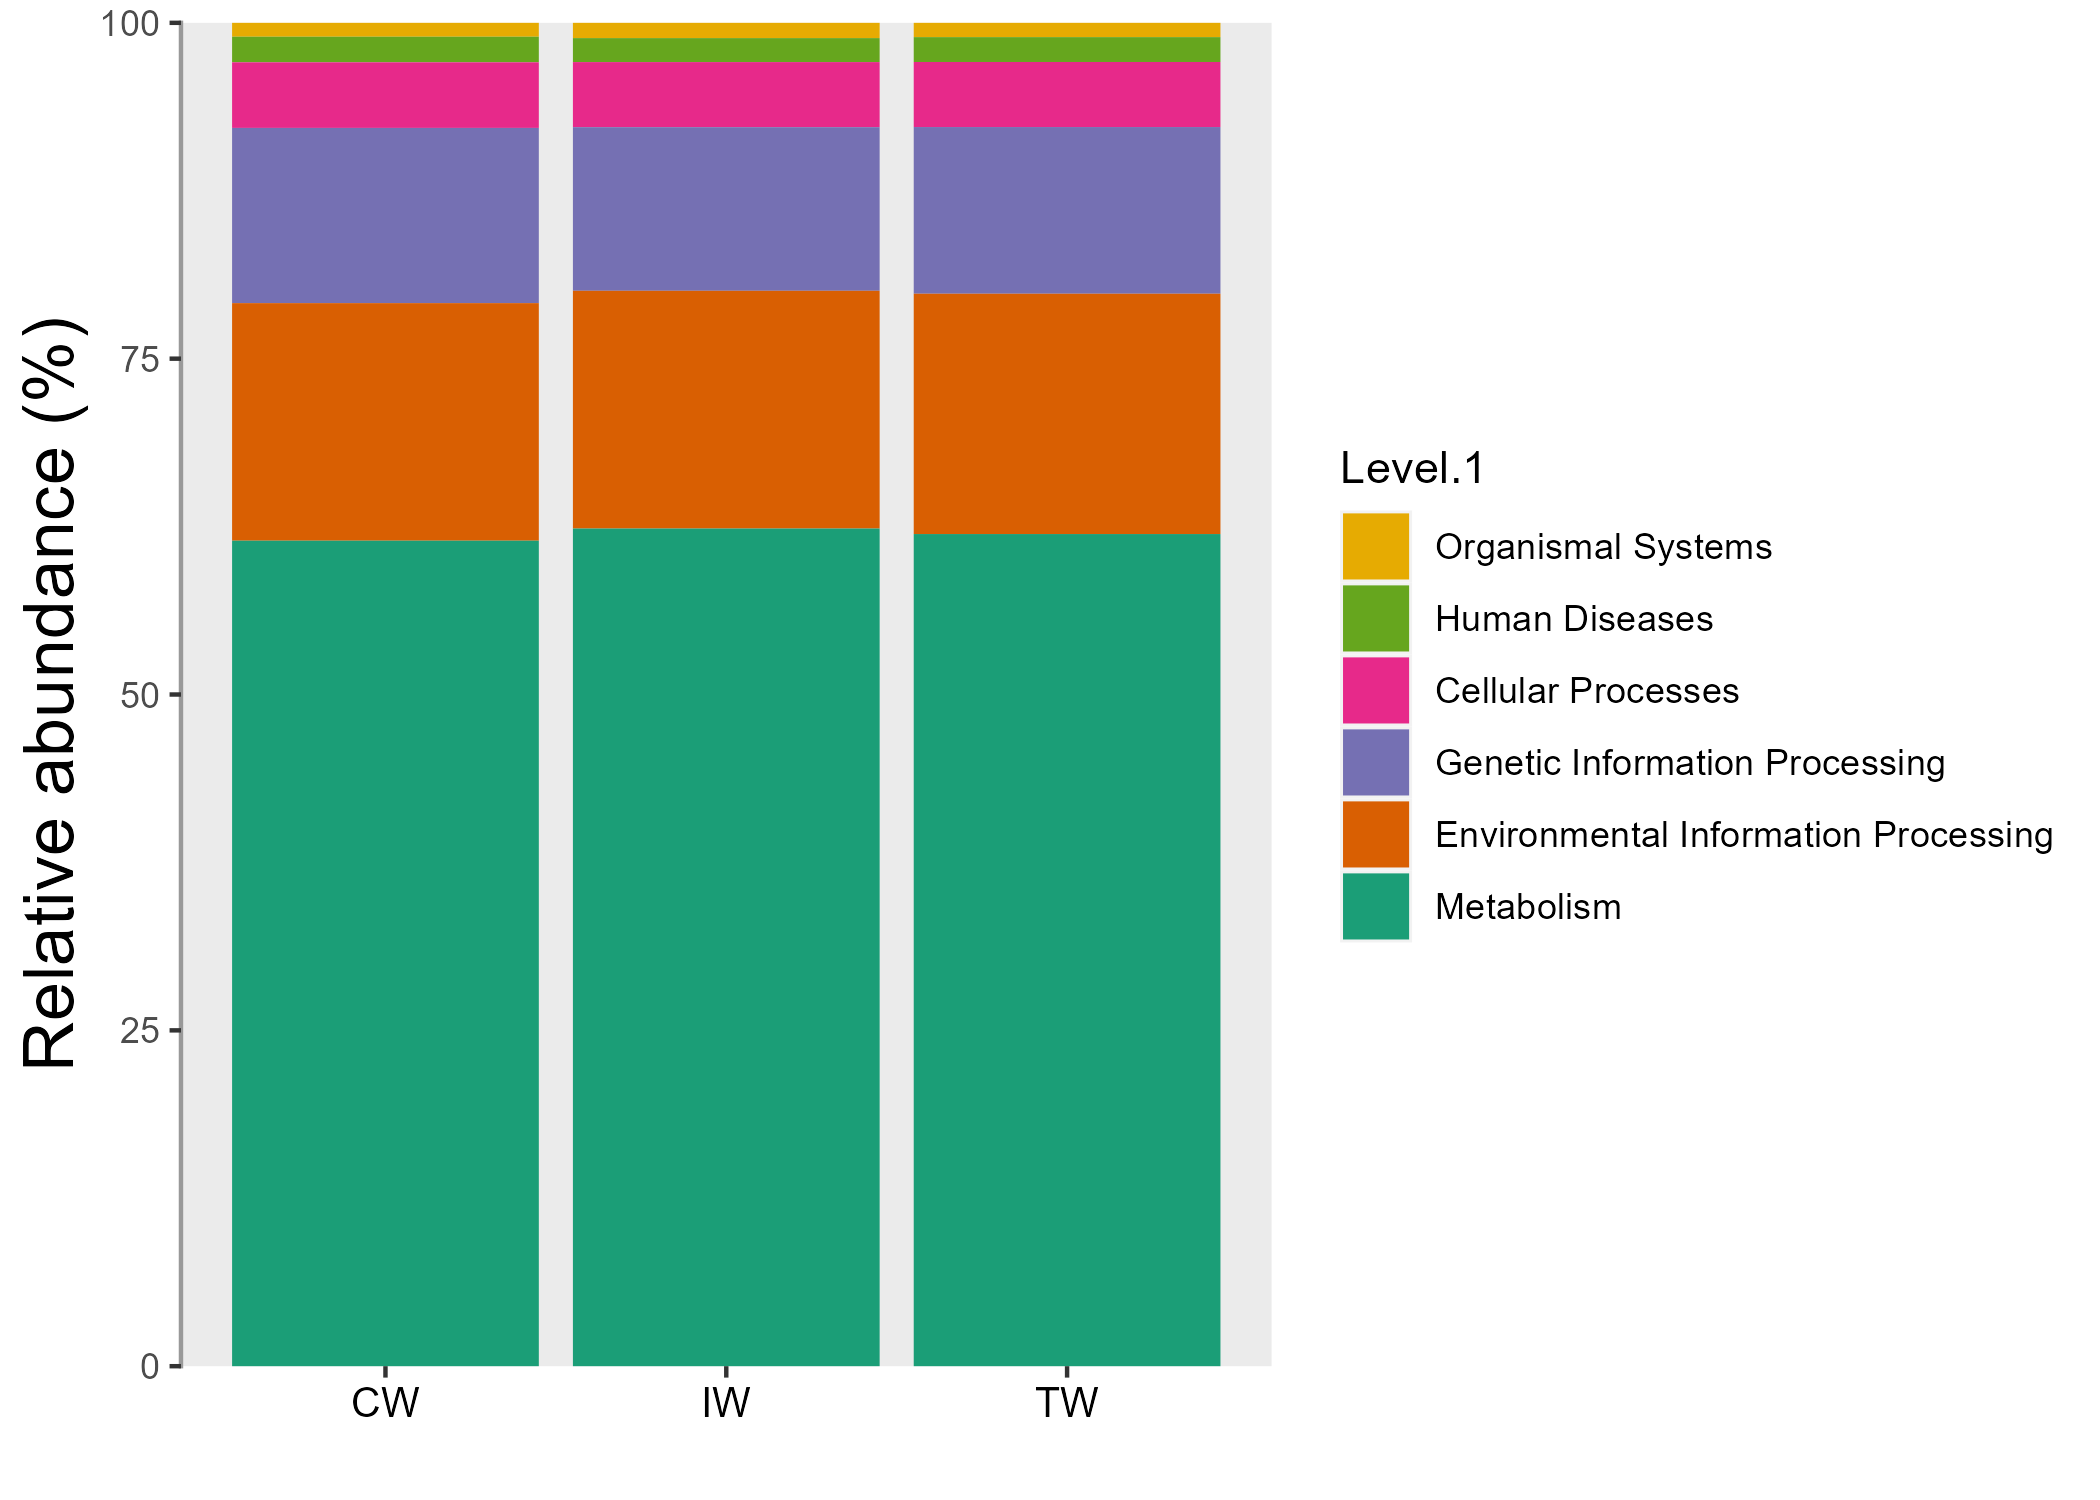
\includegraphics[width=600px]{Images/plot_bar_tax4fun1} \end{center}

We can also do something else. For example, we can use lefse to test the differences of the abundances and find the important enriched pathways across groups.

\begin{Shaded}
\begin{Highlighting}[]
\NormalTok{func2 }\OtherTok{\textless{}{-}}\NormalTok{ trans\_diff}\SpecialCharTok{$}\FunctionTok{new}\NormalTok{(}\AttributeTok{dataset =}\NormalTok{ func1, }\AttributeTok{method =} \StringTok{"lefse"}\NormalTok{, }\AttributeTok{group =} \StringTok{"Group"}\NormalTok{, }\AttributeTok{alpha =} \FloatTok{0.05}\NormalTok{, }\AttributeTok{lefse\_subgroup =} \ConstantTok{NULL}\NormalTok{)}
\NormalTok{func2}\SpecialCharTok{$}\FunctionTok{plot\_lefse\_bar}\NormalTok{(}\AttributeTok{LDA\_score =} \DecValTok{3}\NormalTok{, }\AttributeTok{width =} \FloatTok{0.8}\NormalTok{)}
\end{Highlighting}
\end{Shaded}

\begin{center}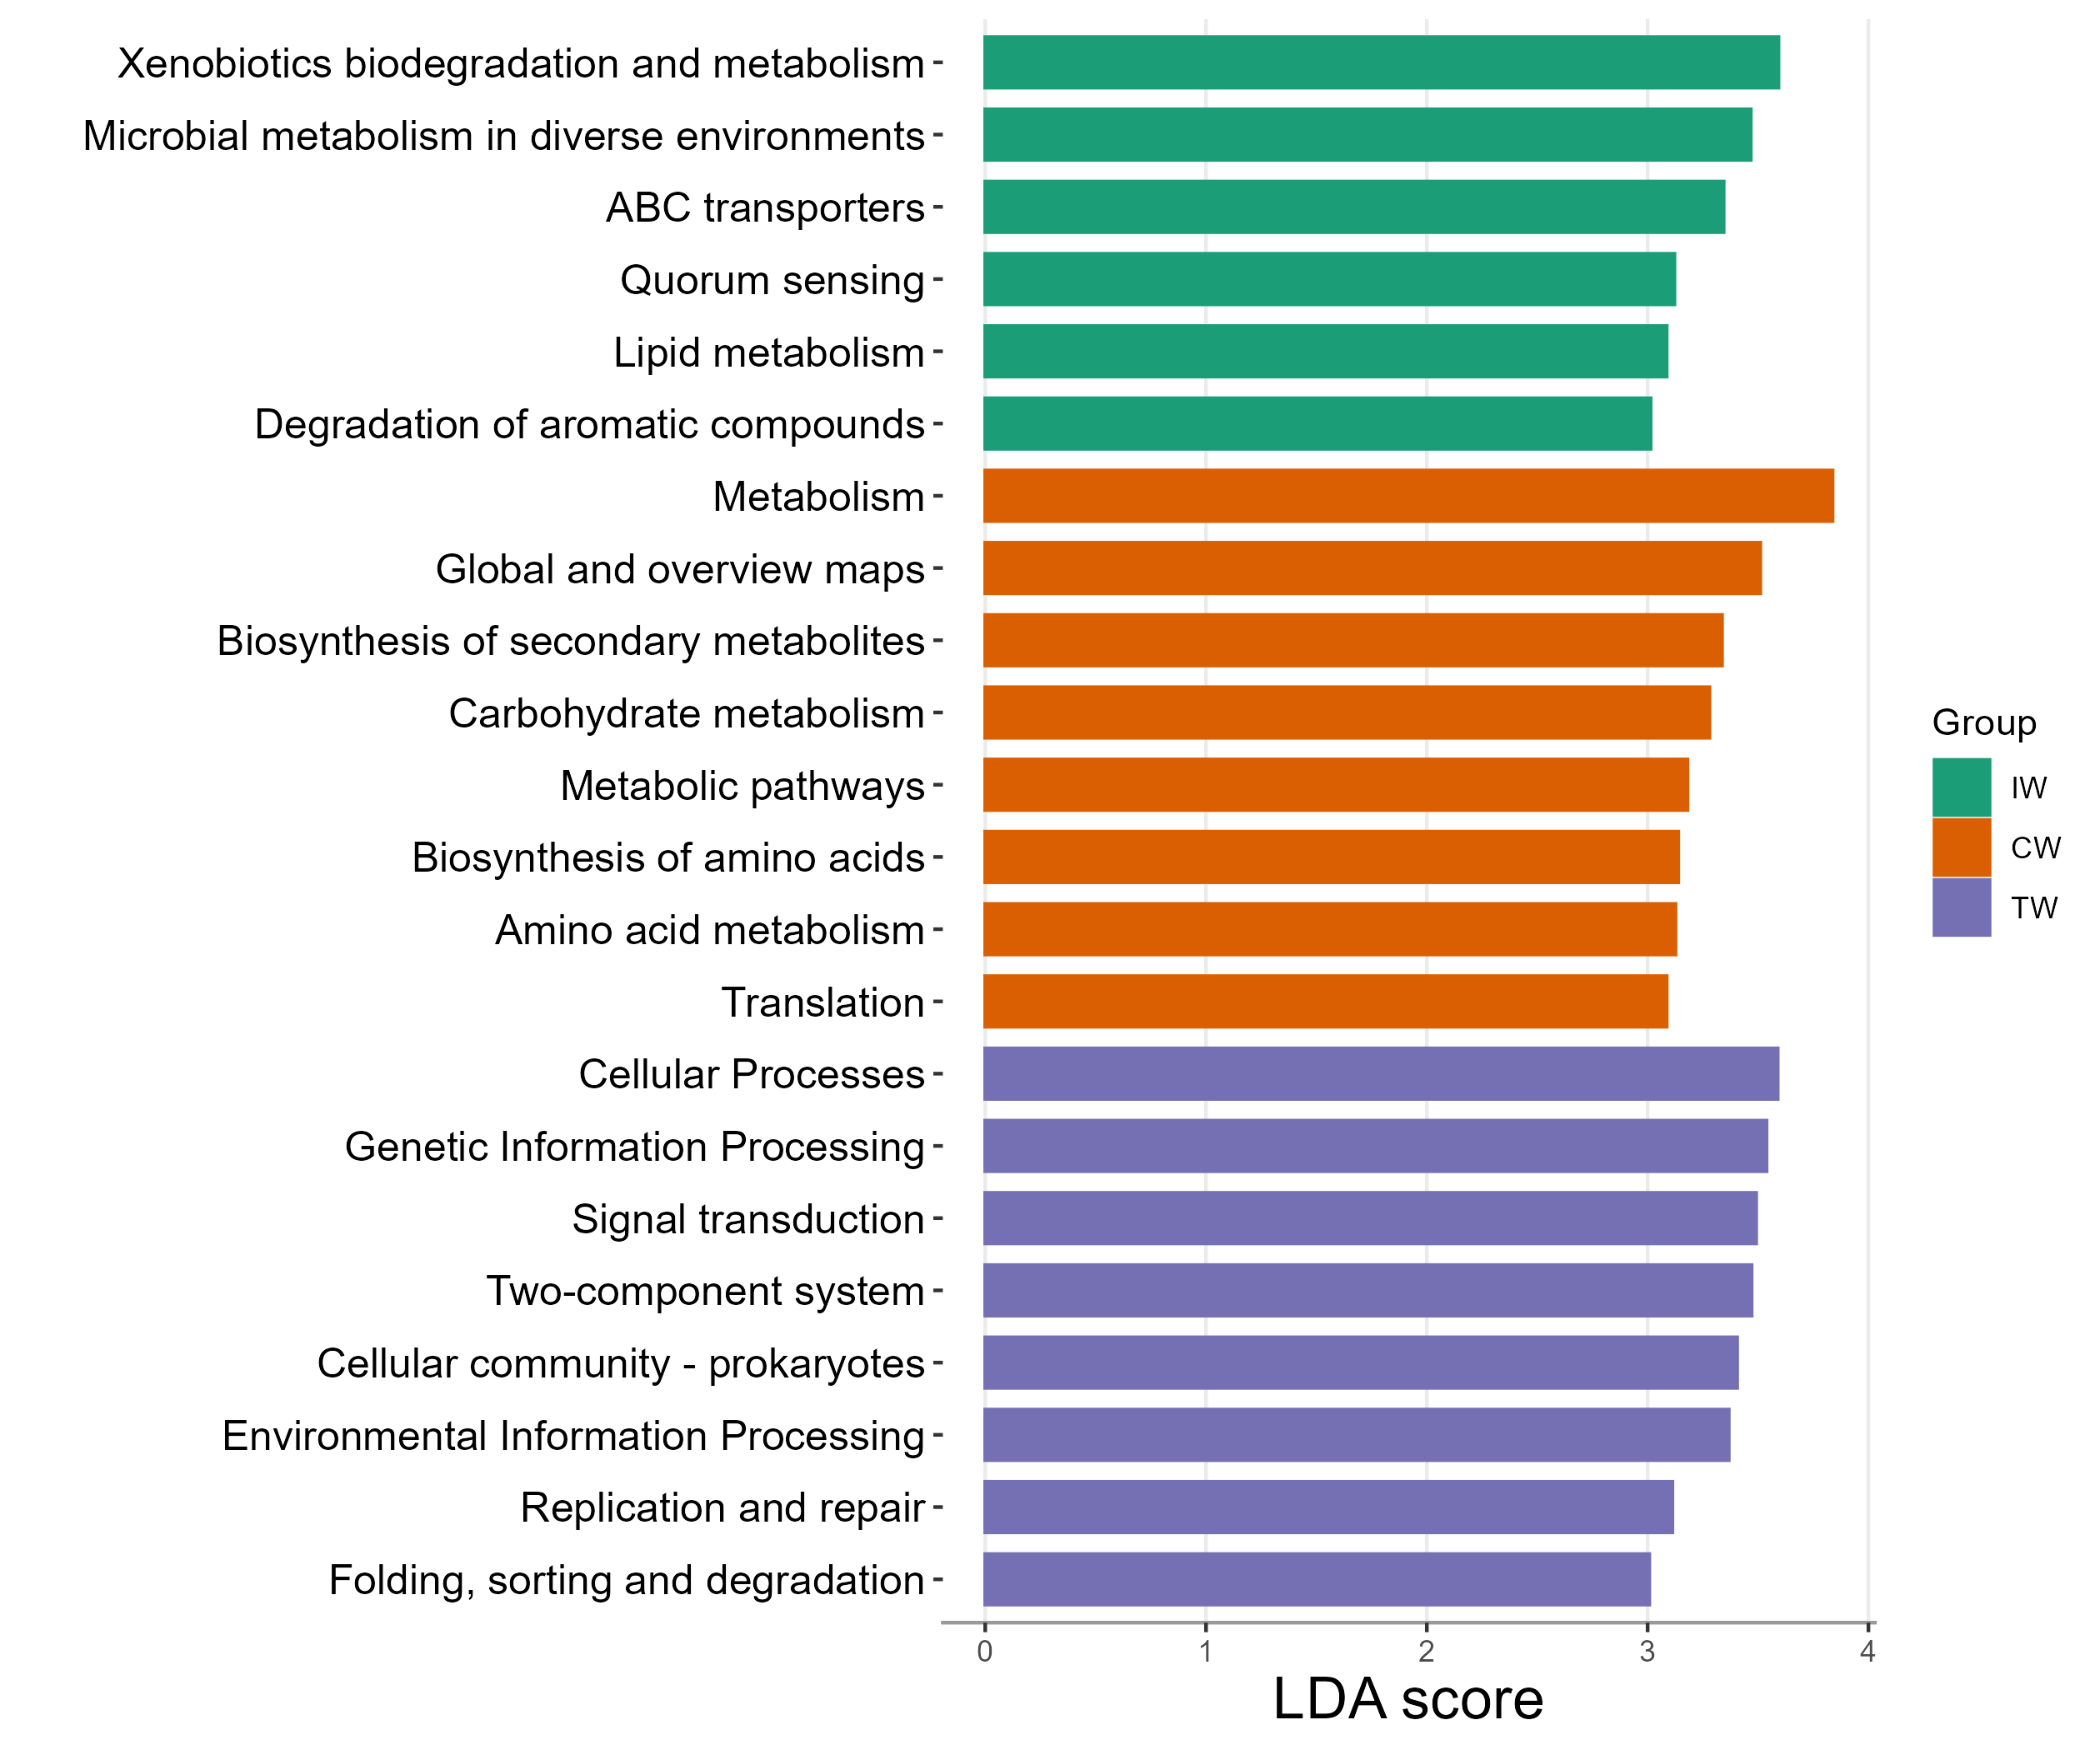
\includegraphics[width=600px]{Images/plot_lefse_bar_tax4fun} \end{center}

Tax4Fun2 \citep{Wemheuer_Tax4Fun2_2020} is another R package for the prediction of functional profiles of prokaryotic communities from 16S rRNA gene sequences.
It can provides two indexes for the evaluation of functional gene redundancies.
We provide two functions cal\_tax4fun2() and cal\_tax4fun2\_FRI() in trans\_func class for the Tax4Fun2 analysis.\\
If you want to use Tax4Fun2 method, you must add the fasta file to the microtable object.

\begin{Shaded}
\begin{Highlighting}[]
\CommentTok{\# create a microtable object with the fasta file}
\FunctionTok{data}\NormalTok{(sample\_info\_16S)}
\FunctionTok{data}\NormalTok{(otu\_table\_16S)}
\FunctionTok{data}\NormalTok{(taxonomy\_table\_16S)}
\FunctionTok{data}\NormalTok{(rep\_fasta\_16S)}

\NormalTok{use\_dataset }\OtherTok{\textless{}{-}}\NormalTok{ microtable}\SpecialCharTok{$}\FunctionTok{new}\NormalTok{(}\AttributeTok{sample\_table =}\NormalTok{ sample\_info\_16S, }\AttributeTok{otu\_table =}\NormalTok{ otu\_table\_16S, }\AttributeTok{tax\_table =}\NormalTok{ taxonomy\_table\_16S, }\AttributeTok{rep\_fasta =}\NormalTok{ rep\_fasta\_16S)}
\NormalTok{use\_dataset}\SpecialCharTok{$}\FunctionTok{filter\_pollution}\NormalTok{(}\AttributeTok{taxa =} \FunctionTok{c}\NormalTok{(}\StringTok{"mitochondria"}\NormalTok{, }\StringTok{"chloroplast"}\NormalTok{))}
\NormalTok{use\_dataset}\SpecialCharTok{$}\FunctionTok{tidy\_dataset}\NormalTok{()}
\NormalTok{use\_dataset}

\NormalTok{t1 }\OtherTok{\textless{}{-}}\NormalTok{ trans\_func}\SpecialCharTok{$}\FunctionTok{new}\NormalTok{(use\_dataset)}
\CommentTok{\# create a directory for result and log files}
\FunctionTok{dir.create}\NormalTok{(}\StringTok{"test\_prediction"}\NormalTok{)}
\CommentTok{\# see https://github.com/ChiLiubio/microeco for downloading ncbi{-}blast and Ref99NR/Ref100NR}
\NormalTok{t1}\SpecialCharTok{$}\FunctionTok{cal\_tax4fun2}\NormalTok{(}\AttributeTok{blast\_tool\_path =} \StringTok{"ncbi{-}blast{-}2.11.0+/bin"}\NormalTok{, }\AttributeTok{path\_to\_reference\_data =} \StringTok{"test\_ReferenceData\_v2"}\NormalTok{,}
  \AttributeTok{path\_to\_temp\_folder =} \StringTok{"test\_prediction"}\NormalTok{, }\AttributeTok{database\_mode =} \StringTok{"Ref99NR"}\NormalTok{)}

\CommentTok{\# functional gene redundancies}
\NormalTok{t1}\SpecialCharTok{$}\FunctionTok{cal\_tax4fun2\_FRI}\NormalTok{()}
\end{Highlighting}
\end{Shaded}

\hypertarget{other-data}{%
\chapter{Other data}\label{other-data}}

\hypertarget{fungi-data}{%
\section{Fungi data}\label{fungi-data}}

The above examples are shown with the prokaryotic data.
Now, we use the ITS amplicon sequencing dataset as an example to show the use of FUNGuild database\citep{Nguyen_FUNGuild_2016}.
FungalTraits \citep{Polme_FungalTraits_2020} database is also available for identifying fungal traits.

\begin{Shaded}
\begin{Highlighting}[]
\CommentTok{\# load ITS data}
\FunctionTok{data}\NormalTok{(sample\_info\_ITS)}
\FunctionTok{data}\NormalTok{(otu\_table\_ITS)}
\FunctionTok{data}\NormalTok{(taxonomy\_table\_ITS)}
\CommentTok{\# create microtable object}
\NormalTok{dataset }\OtherTok{\textless{}{-}}\NormalTok{ microtable}\SpecialCharTok{$}\FunctionTok{new}\NormalTok{(}\AttributeTok{sample\_table =}\NormalTok{ sample\_info\_ITS, }\AttributeTok{otu\_table =}\NormalTok{ otu\_table\_ITS, }\AttributeTok{tax\_table =}\NormalTok{ taxonomy\_table\_ITS)}
\CommentTok{\# remove the taxa not assigned in the Kingdom "k\_\_Fungi"}
\NormalTok{dataset}\SpecialCharTok{$}\NormalTok{tax\_table }\SpecialCharTok{\%\textless{}\textgreater{}\%}\NormalTok{ base}\SpecialCharTok{::}\FunctionTok{subset}\NormalTok{(Kingdom }\SpecialCharTok{==} \StringTok{"k\_\_Fungi"}\NormalTok{)}
\CommentTok{\# use tidy\_dataset() to make OTUs and samples information consistent across files}
\NormalTok{dataset}\SpecialCharTok{$}\FunctionTok{tidy\_dataset}\NormalTok{()}
\CommentTok{\# create trans\_network object}
\NormalTok{t1 }\OtherTok{\textless{}{-}}\NormalTok{ trans\_network}\SpecialCharTok{$}\FunctionTok{new}\NormalTok{(}\AttributeTok{dataset =}\NormalTok{ dataset, }\AttributeTok{cal\_cor =} \StringTok{"WGCNA"}\NormalTok{, }\AttributeTok{taxa\_level =} \StringTok{"OTU"}\NormalTok{, }\AttributeTok{filter\_thres =} \FloatTok{0.000001}\NormalTok{, }\AttributeTok{cor\_method =} \StringTok{"spearman"}\NormalTok{)}
\CommentTok{\# create correlation network }
\NormalTok{t1}\SpecialCharTok{$}\FunctionTok{cal\_network}\NormalTok{(}\AttributeTok{p\_thres =} \FloatTok{0.05}\NormalTok{, }\AttributeTok{COR\_cut =} \FloatTok{0.6}\NormalTok{)}
\CommentTok{\# add modules}
\NormalTok{t1}\SpecialCharTok{$}\FunctionTok{cal\_module}\NormalTok{()}
\CommentTok{\# calculate node topological properties}
\NormalTok{t1}\SpecialCharTok{$}\FunctionTok{cal\_node\_type}\NormalTok{()}
\NormalTok{node\_type\_table }\OtherTok{\textless{}{-}}\NormalTok{ t1}\SpecialCharTok{$}\NormalTok{res\_node\_type}
\CommentTok{\# create trans\_func object}
\NormalTok{t2 }\OtherTok{\textless{}{-}}\NormalTok{ trans\_func}\SpecialCharTok{$}\FunctionTok{new}\NormalTok{(dataset)}
\CommentTok{\# identify species traits, automatically select database for prokaryotes or fungi}
\CommentTok{\# fungi\_database = "FungalTraits" for the FungalTraits database}
\NormalTok{t2}\SpecialCharTok{$}\FunctionTok{cal\_spe\_func}\NormalTok{(}\AttributeTok{fungi\_database =} \StringTok{"FUNGuild"}\NormalTok{)}
\CommentTok{\# calculate abundance{-}unweighted functional redundancy of each trait for each network module}
\NormalTok{t2}\SpecialCharTok{$}\FunctionTok{cal\_spe\_func\_perc}\NormalTok{(}\AttributeTok{use\_community =} \ConstantTok{FALSE}\NormalTok{, }\AttributeTok{node\_type\_table =}\NormalTok{ node\_type\_table)}
\CommentTok{\# plot the functional redundancy of network modules}
\NormalTok{t2}\SpecialCharTok{$}\FunctionTok{plot\_spe\_func\_perc}\NormalTok{(}\AttributeTok{select\_samples =} \FunctionTok{paste0}\NormalTok{(}\StringTok{"M"}\NormalTok{, }\DecValTok{1}\SpecialCharTok{:}\DecValTok{10}\NormalTok{))}
\end{Highlighting}
\end{Shaded}

\begin{center}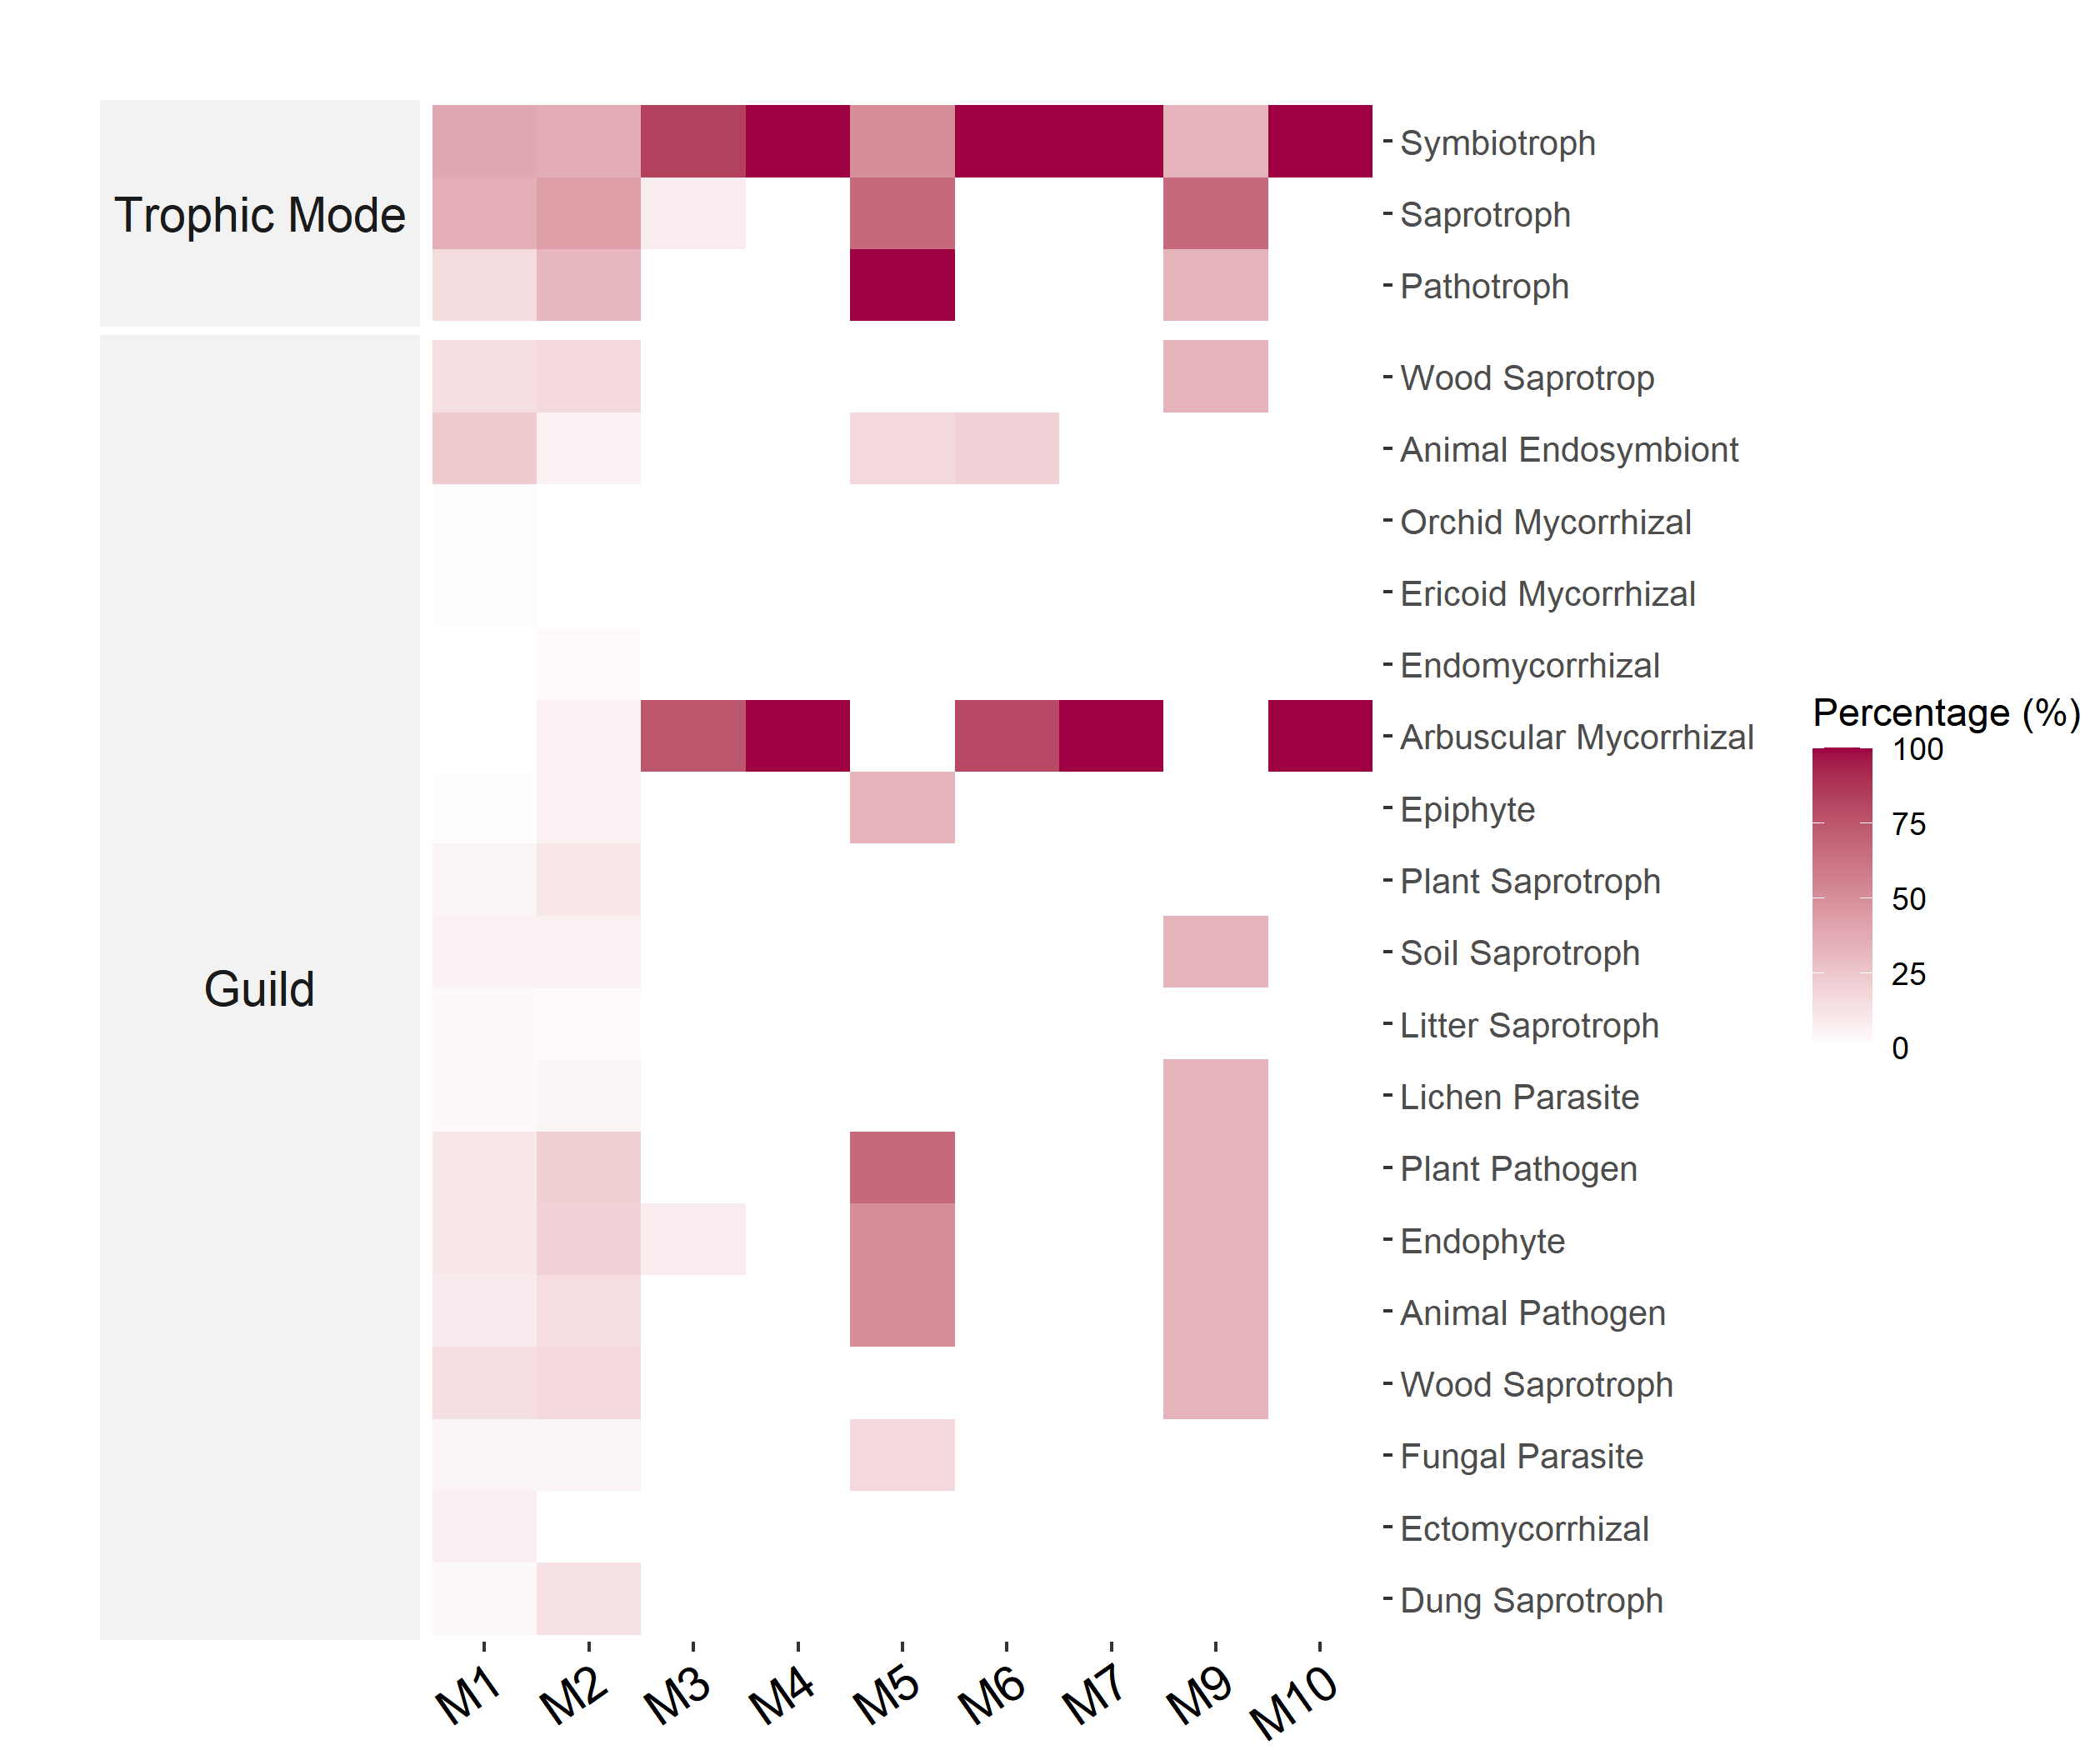
\includegraphics[width=700px]{Images/plot_func_perc_module_fungi} \end{center}

\hypertarget{metagenomic-data}{%
\section{Metagenomic data}\label{metagenomic-data}}

Many methods in microeco package can be used not only for the traditional species abundance data, i.e.~species-sample table,
but also for other data, such as metagenomic and metabolomic data.
In the file2meco package (\url{https://github.com/ChiLiubio/file2meco}),
we provide several functions to transform the output files of some famous metagenomic tools (e.g.~HUMAnN) to
the microtable object directly.
HUMAnN\citep{Franzosa_Species_2018} is an excellent tool for functional profiling analysis of metagenomes and metatranscriptomes at species-level.
Certainly, it can also be used for the whole community profile of metabolic pathways if you do not need something at species-level.
The humann2meco() function can be used to creat the microtable object using metagenomic analysis files from HUMAnN2 and HUMAnN3 (\url{https://huttenhower.sph.harvard.edu/humann}).
Currently, it supports both the MetaCyc (\url{https://metacyc.org/}) and KEGG pathway abundance file input.
Here, we show the example of KEGG pathway results.

\begin{Shaded}
\begin{Highlighting}[]
\FunctionTok{library}\NormalTok{(microeco)}
\FunctionTok{library}\NormalTok{(file2meco)}
\FunctionTok{library}\NormalTok{(magrittr)}
\NormalTok{?humann2meco}
\NormalTok{sample\_file\_path }\OtherTok{\textless{}{-}} \FunctionTok{system.file}\NormalTok{(}\StringTok{"extdata"}\NormalTok{, }\StringTok{"example\_metagenome\_sample\_info.tsv"}\NormalTok{, }\AttributeTok{package=}\StringTok{"file2meco"}\NormalTok{)}
\NormalTok{match\_file\_path }\OtherTok{\textless{}{-}} \FunctionTok{system.file}\NormalTok{(}\StringTok{"extdata"}\NormalTok{, }\StringTok{"example\_metagenome\_match\_table.tsv"}\NormalTok{, }\AttributeTok{package=}\StringTok{"file2meco"}\NormalTok{)}
\CommentTok{\# use KEGG pathway based HUMAnN result}
\NormalTok{abund\_file\_path }\OtherTok{\textless{}{-}} \FunctionTok{system.file}\NormalTok{(}\StringTok{"extdata"}\NormalTok{, }\StringTok{"example\_HUMAnN\_KEGG\_abund.tsv"}\NormalTok{, }\AttributeTok{package=}\StringTok{"file2meco"}\NormalTok{)}
\NormalTok{test }\OtherTok{\textless{}{-}} \FunctionTok{humann2meco}\NormalTok{(}\AttributeTok{abund\_table =}\NormalTok{ abund\_file\_path, }\AttributeTok{db =} \StringTok{"KEGG"}\NormalTok{, }\AttributeTok{sample\_data =}\NormalTok{ sample\_file\_path, }\AttributeTok{match\_table =}\NormalTok{ match\_file\_path)}
\CommentTok{\# remove the unclassified pathway in the top level}
\NormalTok{test}\SpecialCharTok{$}\NormalTok{tax\_table }\SpecialCharTok{\%\textless{}\textgreater{}\%} \FunctionTok{subset}\NormalTok{(level1 }\SpecialCharTok{!=} \StringTok{"unclassified"}\NormalTok{)}
\NormalTok{test}\SpecialCharTok{$}\FunctionTok{tidy\_dataset}\NormalTok{()}
\CommentTok{\# rel = FALSE donot use relative abundance, use the raw RPK}
\NormalTok{test}\SpecialCharTok{$}\FunctionTok{cal\_abund}\NormalTok{(}\AttributeTok{select\_cols =} \DecValTok{1}\SpecialCharTok{:}\DecValTok{3}\NormalTok{, }\AttributeTok{rel =} \ConstantTok{FALSE}\NormalTok{)}
\NormalTok{test1 }\OtherTok{\textless{}{-}}\NormalTok{ trans\_abund}\SpecialCharTok{$}\FunctionTok{new}\NormalTok{(test, }\AttributeTok{taxrank =} \StringTok{"level2"}\NormalTok{, }\AttributeTok{ntaxa =} \DecValTok{10}\NormalTok{)}
\NormalTok{test1}\SpecialCharTok{$}\FunctionTok{plot\_bar}\NormalTok{(}\AttributeTok{facet =} \StringTok{"Group"}\NormalTok{, }\AttributeTok{ylab\_title =} \StringTok{"Abundance (RPK)"}\NormalTok{, }\AttributeTok{use\_colors =}\NormalTok{ RColorBrewer}\SpecialCharTok{::}\FunctionTok{brewer.pal}\NormalTok{(}\DecValTok{12}\NormalTok{, }\StringTok{"Set3"}\NormalTok{))}
\end{Highlighting}
\end{Shaded}

\begin{center}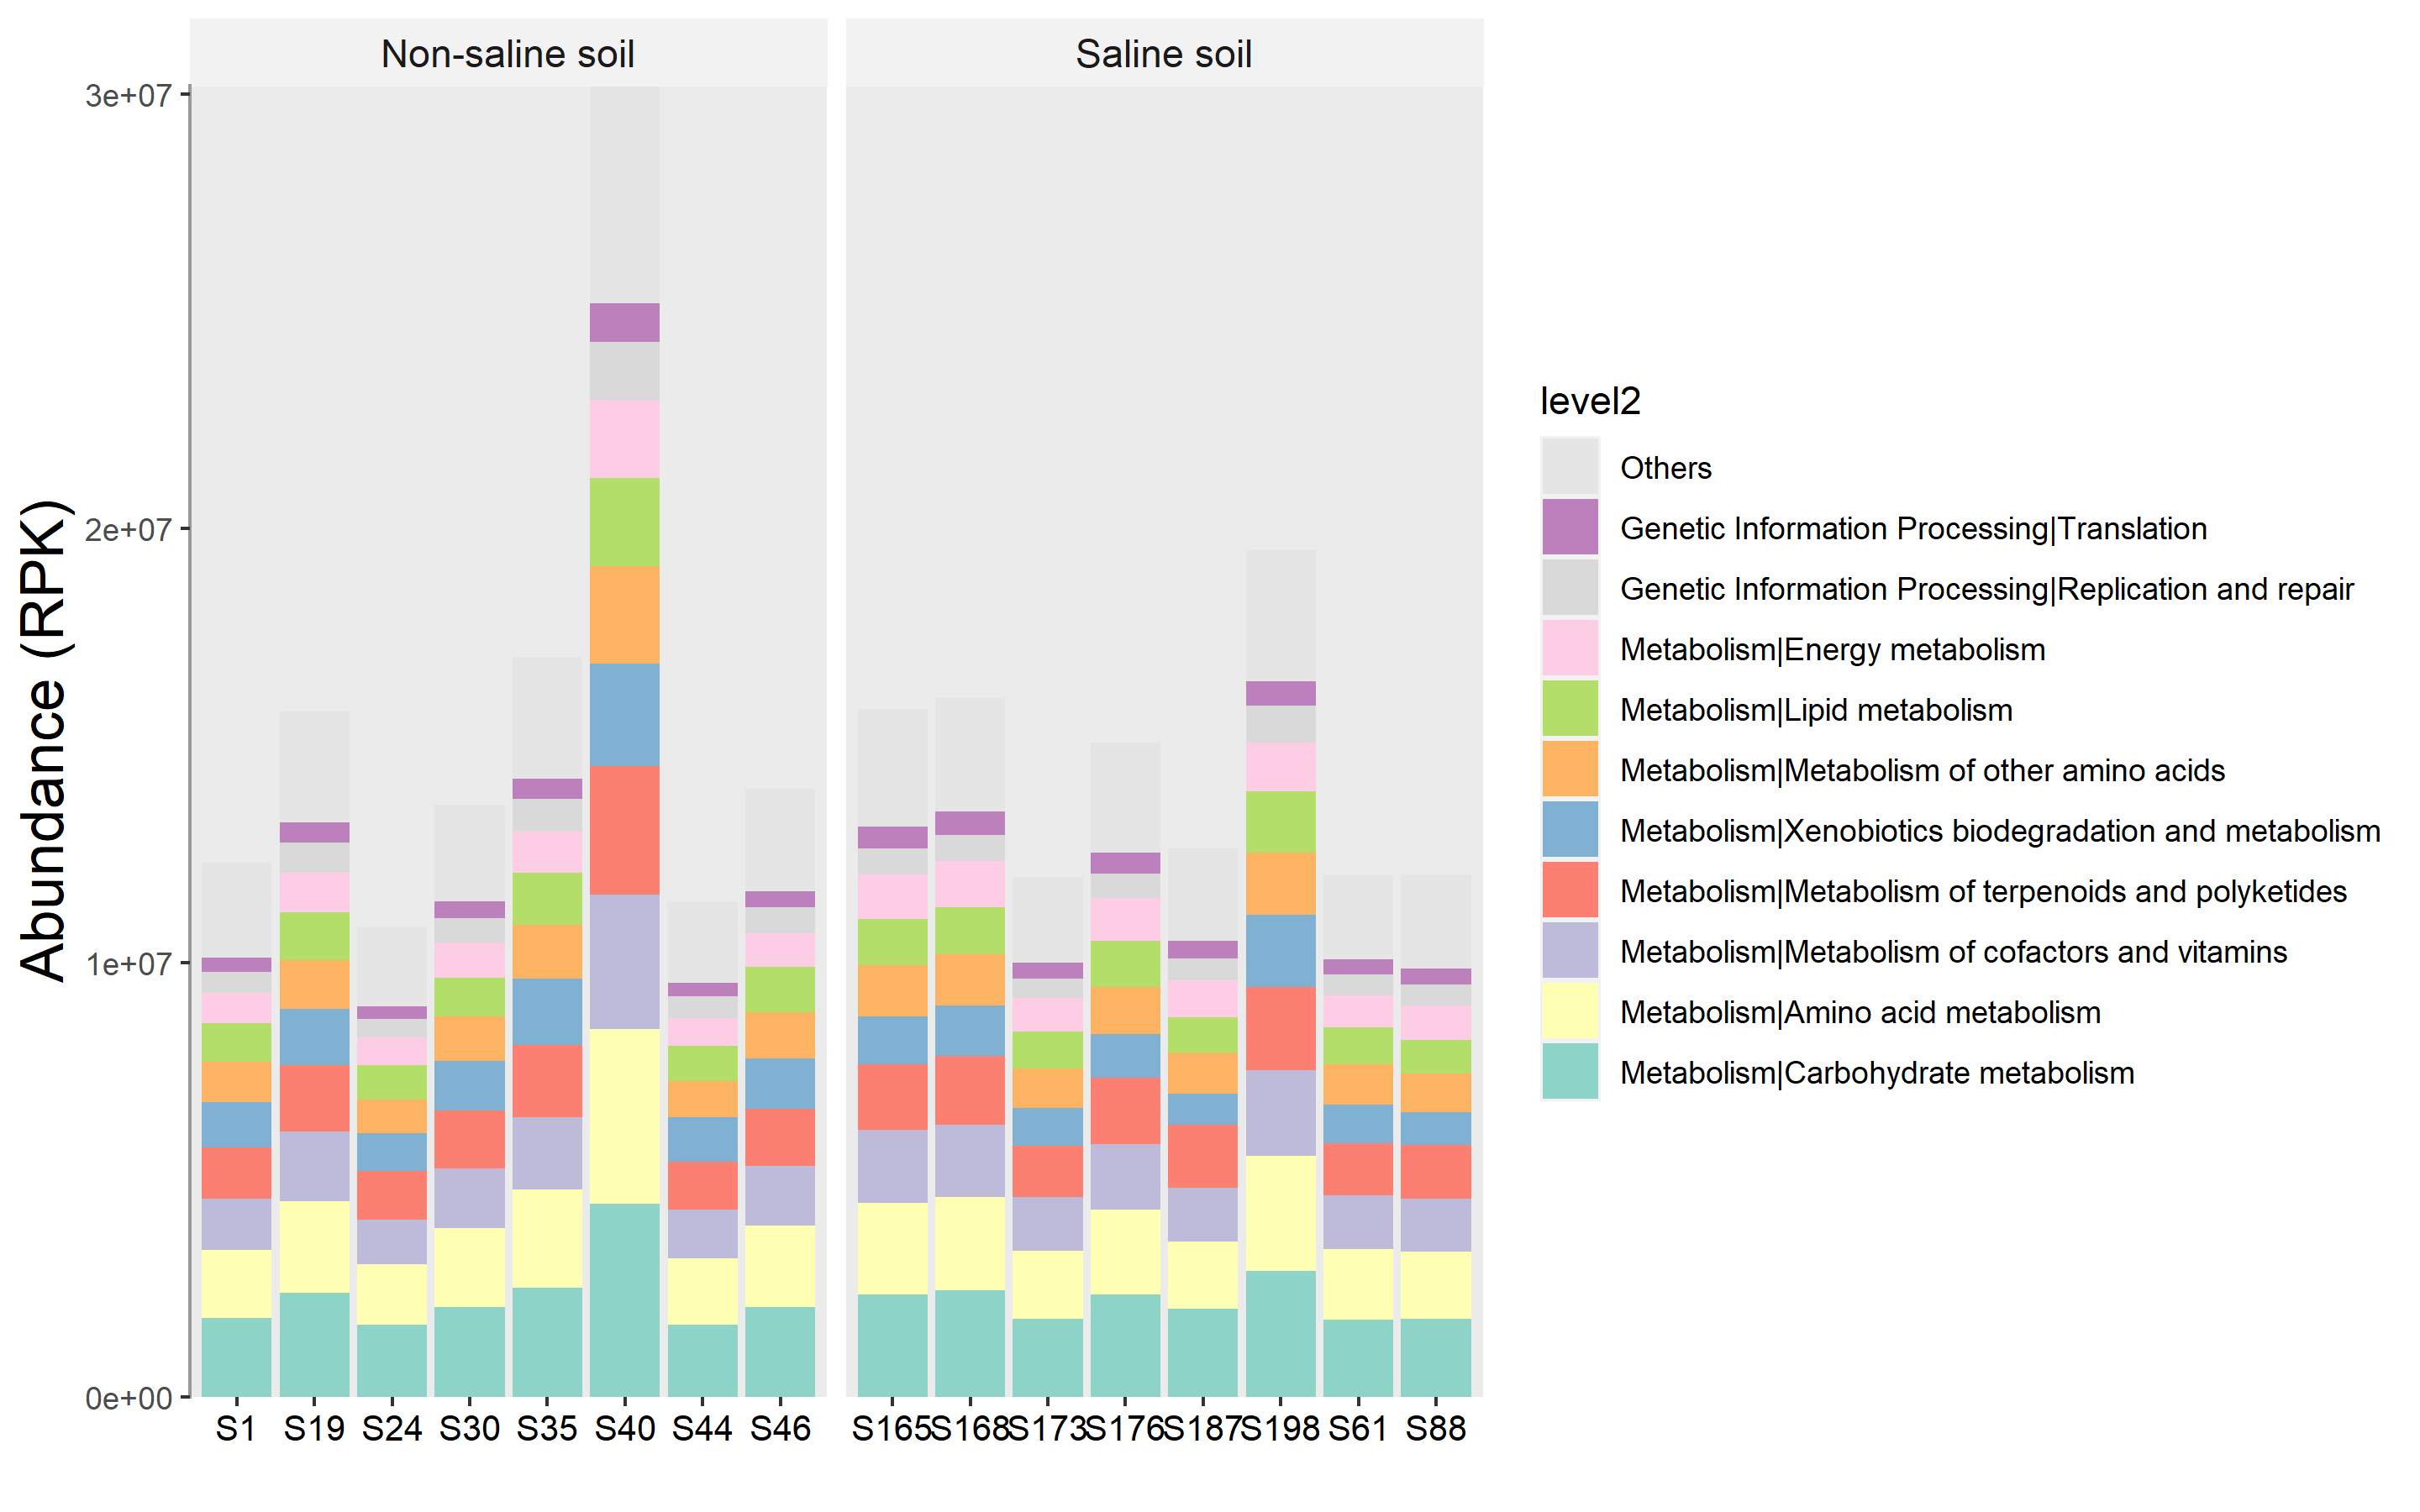
\includegraphics[width=800px]{Images/plot_HUMANN_KEGG_bar} \end{center}

Then, we select both function and taxa to see which taxa the high abundant pathways come from.

\begin{Shaded}
\begin{Highlighting}[]
\CommentTok{\# This operation is more flexible}
\NormalTok{test}\SpecialCharTok{$}\FunctionTok{cal\_abund}\NormalTok{(}\AttributeTok{select\_cols =} \FunctionTok{c}\NormalTok{(}\StringTok{"level1"}\NormalTok{, }\StringTok{"Phylum"}\NormalTok{, }\StringTok{"Genus"}\NormalTok{), }\AttributeTok{rel =} \ConstantTok{FALSE}\NormalTok{)}
\NormalTok{test}\SpecialCharTok{$}\NormalTok{taxa\_abund}\SpecialCharTok{$}\NormalTok{level1 }\SpecialCharTok{\%\textless{}\textgreater{}\%}\NormalTok{ .[}\SpecialCharTok{!}\FunctionTok{grepl}\NormalTok{(}\StringTok{"unclass"}\NormalTok{, }\FunctionTok{rownames}\NormalTok{(.)), ]}
\NormalTok{test}\SpecialCharTok{$}\NormalTok{taxa\_abund}\SpecialCharTok{$}\NormalTok{Phylum }\SpecialCharTok{\%\textless{}\textgreater{}\%}\NormalTok{ .[}\SpecialCharTok{!}\FunctionTok{grepl}\NormalTok{(}\StringTok{"unclass"}\NormalTok{, }\FunctionTok{rownames}\NormalTok{(.)), ]}
\NormalTok{test1 }\OtherTok{\textless{}{-}}\NormalTok{ trans\_abund}\SpecialCharTok{$}\FunctionTok{new}\NormalTok{(test, }\AttributeTok{taxrank =} \StringTok{"Phylum"}\NormalTok{, }\AttributeTok{ntaxa =} \DecValTok{10}\NormalTok{, }\AttributeTok{delete\_part\_prefix =}\NormalTok{ T)}
\NormalTok{test1}\SpecialCharTok{$}\FunctionTok{plot\_bar}\NormalTok{(}\AttributeTok{facet =} \StringTok{"Group"}\NormalTok{, }\AttributeTok{ylab\_title =} \StringTok{"Abundance (RPK)"}\NormalTok{, }\AttributeTok{use\_colors =}\NormalTok{ RColorBrewer}\SpecialCharTok{::}\FunctionTok{brewer.pal}\NormalTok{(}\DecValTok{12}\NormalTok{, }\StringTok{"Set3"}\NormalTok{))}
\end{Highlighting}
\end{Shaded}

\begin{center}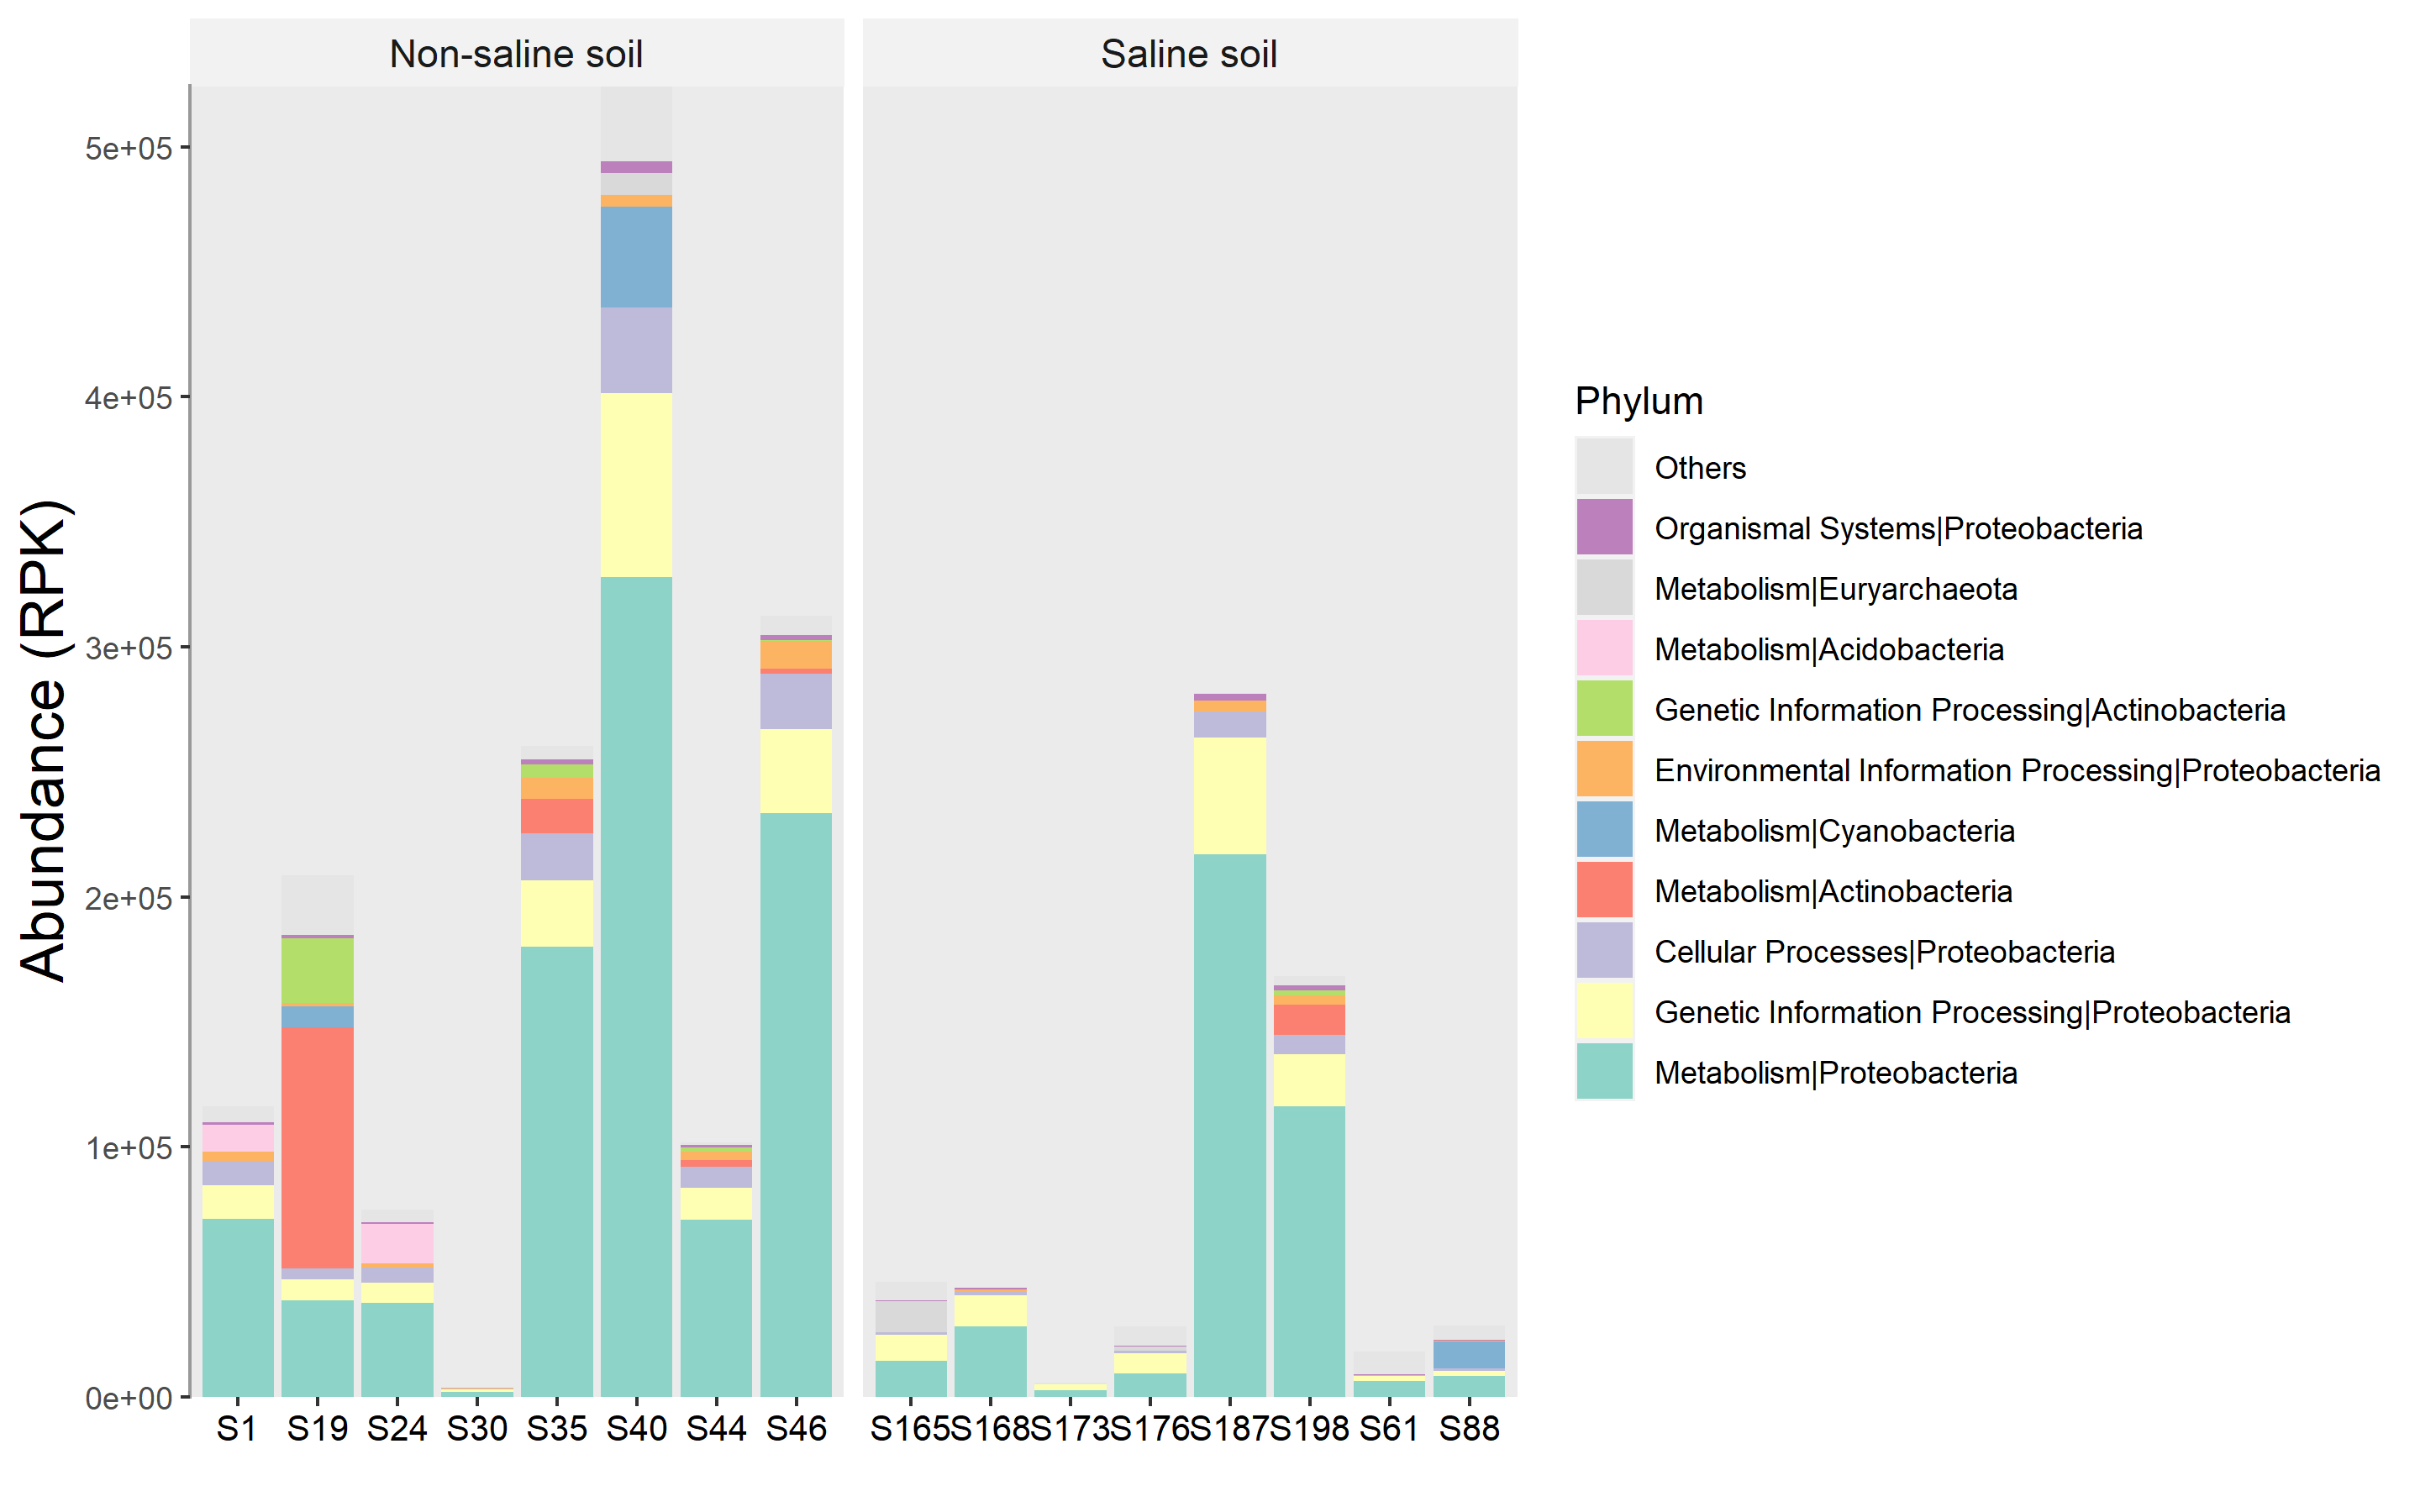
\includegraphics[width=800px]{Images/plot_HUMANN_KEGG_bar_taxafunc} \end{center}

Let's run LEfSe to find some functional biomarkers to differentiate two groups.

\begin{Shaded}
\begin{Highlighting}[]
\CommentTok{\# functional biomarker}
\NormalTok{test}\SpecialCharTok{$}\FunctionTok{cal\_abund}\NormalTok{(}\AttributeTok{select\_cols =} \DecValTok{1}\SpecialCharTok{:}\DecValTok{3}\NormalTok{, }\AttributeTok{rel =} \ConstantTok{TRUE}\NormalTok{)}
\NormalTok{test1 }\OtherTok{\textless{}{-}}\NormalTok{ trans\_diff}\SpecialCharTok{$}\FunctionTok{new}\NormalTok{(test, }\AttributeTok{method =} \StringTok{"lefse"}\NormalTok{, }\AttributeTok{group =} \StringTok{"Group"}\NormalTok{)}
\NormalTok{test1}\SpecialCharTok{$}\FunctionTok{plot\_lefse\_bar}\NormalTok{(}\AttributeTok{LDA\_score =} \DecValTok{3}\NormalTok{)}
\end{Highlighting}
\end{Shaded}

\begin{center}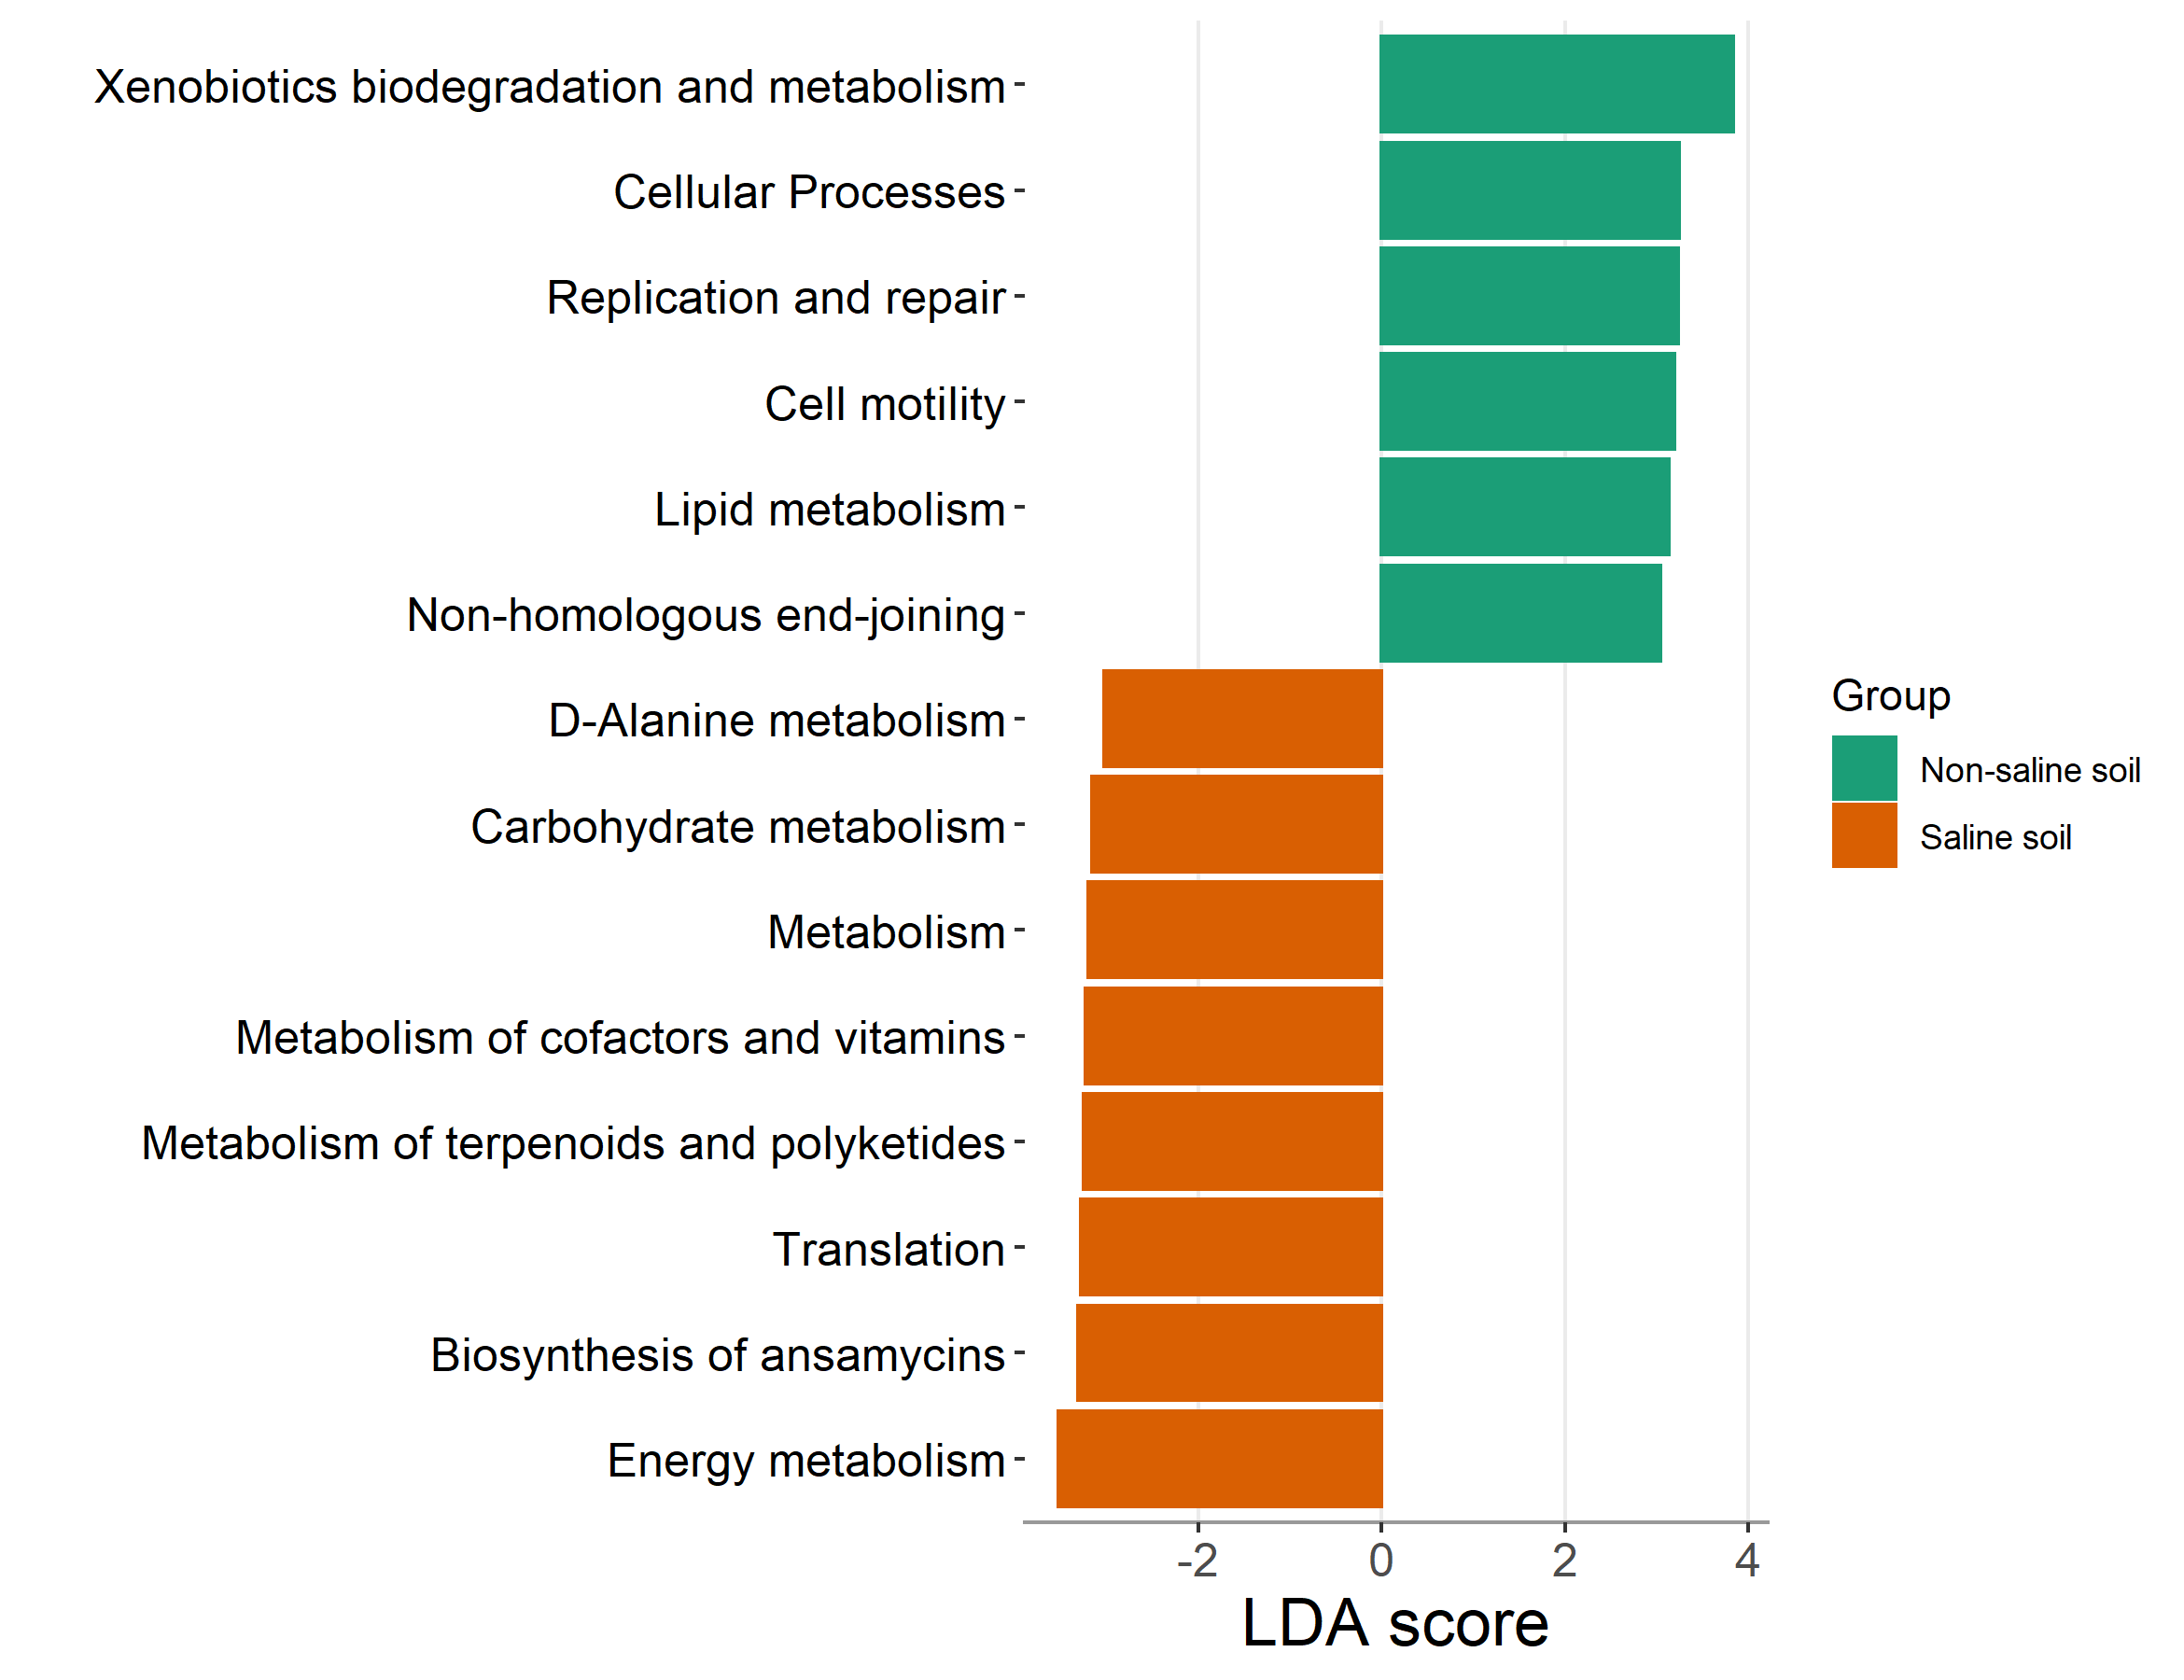
\includegraphics[width=700px]{Images/plot_HUMANN_KEGG_lefse_bar} \end{center}

\hypertarget{animal-data}{%
\section{Animal data}\label{animal-data}}

We use mouse gut data stored in file2meco package to show the input of QIIME2 file and the use of metabolic trait database NJC19 database\citep{Lim_Large_2020}.

\begin{Shaded}
\begin{Highlighting}[]
\FunctionTok{library}\NormalTok{(microeco)}
\FunctionTok{library}\NormalTok{(file2meco)}
\FunctionTok{library}\NormalTok{(ggplot2)}

\CommentTok{\# use data files inside the file2meco package.}
\NormalTok{abund\_file\_path }\OtherTok{\textless{}{-}} \FunctionTok{system.file}\NormalTok{(}\StringTok{"extdata"}\NormalTok{, }\StringTok{"dada2\_table.qza"}\NormalTok{, }\AttributeTok{package=}\StringTok{"file2meco"}\NormalTok{)}
\NormalTok{sample\_file\_path }\OtherTok{\textless{}{-}} \FunctionTok{system.file}\NormalTok{(}\StringTok{"extdata"}\NormalTok{, }\StringTok{"sample{-}metadata.tsv"}\NormalTok{, }\AttributeTok{package=}\StringTok{"file2meco"}\NormalTok{)}
\NormalTok{taxonomy\_file\_path }\OtherTok{\textless{}{-}} \FunctionTok{system.file}\NormalTok{(}\StringTok{"extdata"}\NormalTok{, }\StringTok{"taxonomy.qza"}\NormalTok{, }\AttributeTok{package=}\StringTok{"file2meco"}\NormalTok{)}
\CommentTok{\# construct microtable object}
\NormalTok{data1 }\OtherTok{\textless{}{-}} \FunctionTok{qiime2meco}\NormalTok{(}\AttributeTok{ASV\_data =}\NormalTok{ abund\_file\_path, }\AttributeTok{sample\_data =}\NormalTok{ sample\_file\_path, }\AttributeTok{taxonomy\_data =}\NormalTok{ taxonomy\_file\_path)}
\NormalTok{data1}\SpecialCharTok{$}\FunctionTok{tidy\_dataset}\NormalTok{()}
\CommentTok{\# We correct the species names in tax\_table}
\NormalTok{select\_rows }\OtherTok{\textless{}{-}}\NormalTok{ data1}\SpecialCharTok{$}\NormalTok{tax\_table}\SpecialCharTok{$}\NormalTok{Species }\SpecialCharTok{!=} \StringTok{"s\_\_"}
\NormalTok{data1}\SpecialCharTok{$}\NormalTok{tax\_table}\SpecialCharTok{$}\NormalTok{Species[select\_rows] }\OtherTok{\textless{}{-}} \FunctionTok{paste0}\NormalTok{(}\StringTok{"s\_\_"}\NormalTok{, }\FunctionTok{gsub}\NormalTok{(}\StringTok{"g\_\_"}\NormalTok{, }\StringTok{""}\NormalTok{, data1}\SpecialCharTok{$}\NormalTok{tax\_table}\SpecialCharTok{$}\NormalTok{Genus[select\_rows]), }\StringTok{" "}\NormalTok{, }\FunctionTok{gsub}\NormalTok{(}\StringTok{"s\_\_"}\NormalTok{, }\StringTok{""}\NormalTok{, data1}\SpecialCharTok{$}\NormalTok{tax\_table}\SpecialCharTok{$}\NormalTok{Species[select\_rows]))}
\CommentTok{\# taxonomic abundance}
\NormalTok{data1}\SpecialCharTok{$}\FunctionTok{cal\_abund}\NormalTok{()}

\CommentTok{\# create object of trans\_func}
\NormalTok{data2 }\OtherTok{\textless{}{-}}\NormalTok{ trans\_func}\SpecialCharTok{$}\FunctionTok{new}\NormalTok{(data1)}
\CommentTok{\# Select NJC19 database}
\NormalTok{data2}\SpecialCharTok{$}\FunctionTok{cal\_spe\_func}\NormalTok{(}\AttributeTok{prok\_database =} \StringTok{"NJC19"}\NormalTok{)}
\CommentTok{\# get the trait percentage data}
\NormalTok{data2}\SpecialCharTok{$}\FunctionTok{cal\_spe\_func\_perc}\NormalTok{(}\AttributeTok{use\_community =} \ConstantTok{TRUE}\NormalTok{)}

\CommentTok{\# inset the trait percentage result into taxa\_abund of microtable object}
\NormalTok{data1}\SpecialCharTok{$}\NormalTok{taxa\_abund}\SpecialCharTok{$}\NormalTok{Trait }\OtherTok{\textless{}{-}} \FunctionTok{as.data.frame}\NormalTok{(}\FunctionTok{t}\NormalTok{(data2}\SpecialCharTok{$}\NormalTok{res\_spe\_func\_perc))}
\CommentTok{\# use trans\_abund to plot}
\NormalTok{t1 }\OtherTok{\textless{}{-}}\NormalTok{ trans\_abund}\SpecialCharTok{$}\FunctionTok{new}\NormalTok{(}\AttributeTok{dataset =}\NormalTok{ data1, }\AttributeTok{taxrank =} \StringTok{"Trait"}\NormalTok{, }\AttributeTok{ntaxa =} \DecValTok{10}\NormalTok{, }\AttributeTok{use\_percentage =} \ConstantTok{FALSE}\NormalTok{)}
\NormalTok{t1}\SpecialCharTok{$}\FunctionTok{plot\_box}\NormalTok{(}\AttributeTok{group =} \StringTok{"donor\_status"}\NormalTok{) }\SpecialCharTok{+} \FunctionTok{ylab}\NormalTok{(}\StringTok{"Relative population abundance (\%)"}\NormalTok{) }\SpecialCharTok{+} \FunctionTok{theme}\NormalTok{(}\AttributeTok{axis.text.x =} \FunctionTok{element\_text}\NormalTok{(}\AttributeTok{size =} \DecValTok{13}\NormalTok{))}
\end{Highlighting}
\end{Shaded}

\begin{center}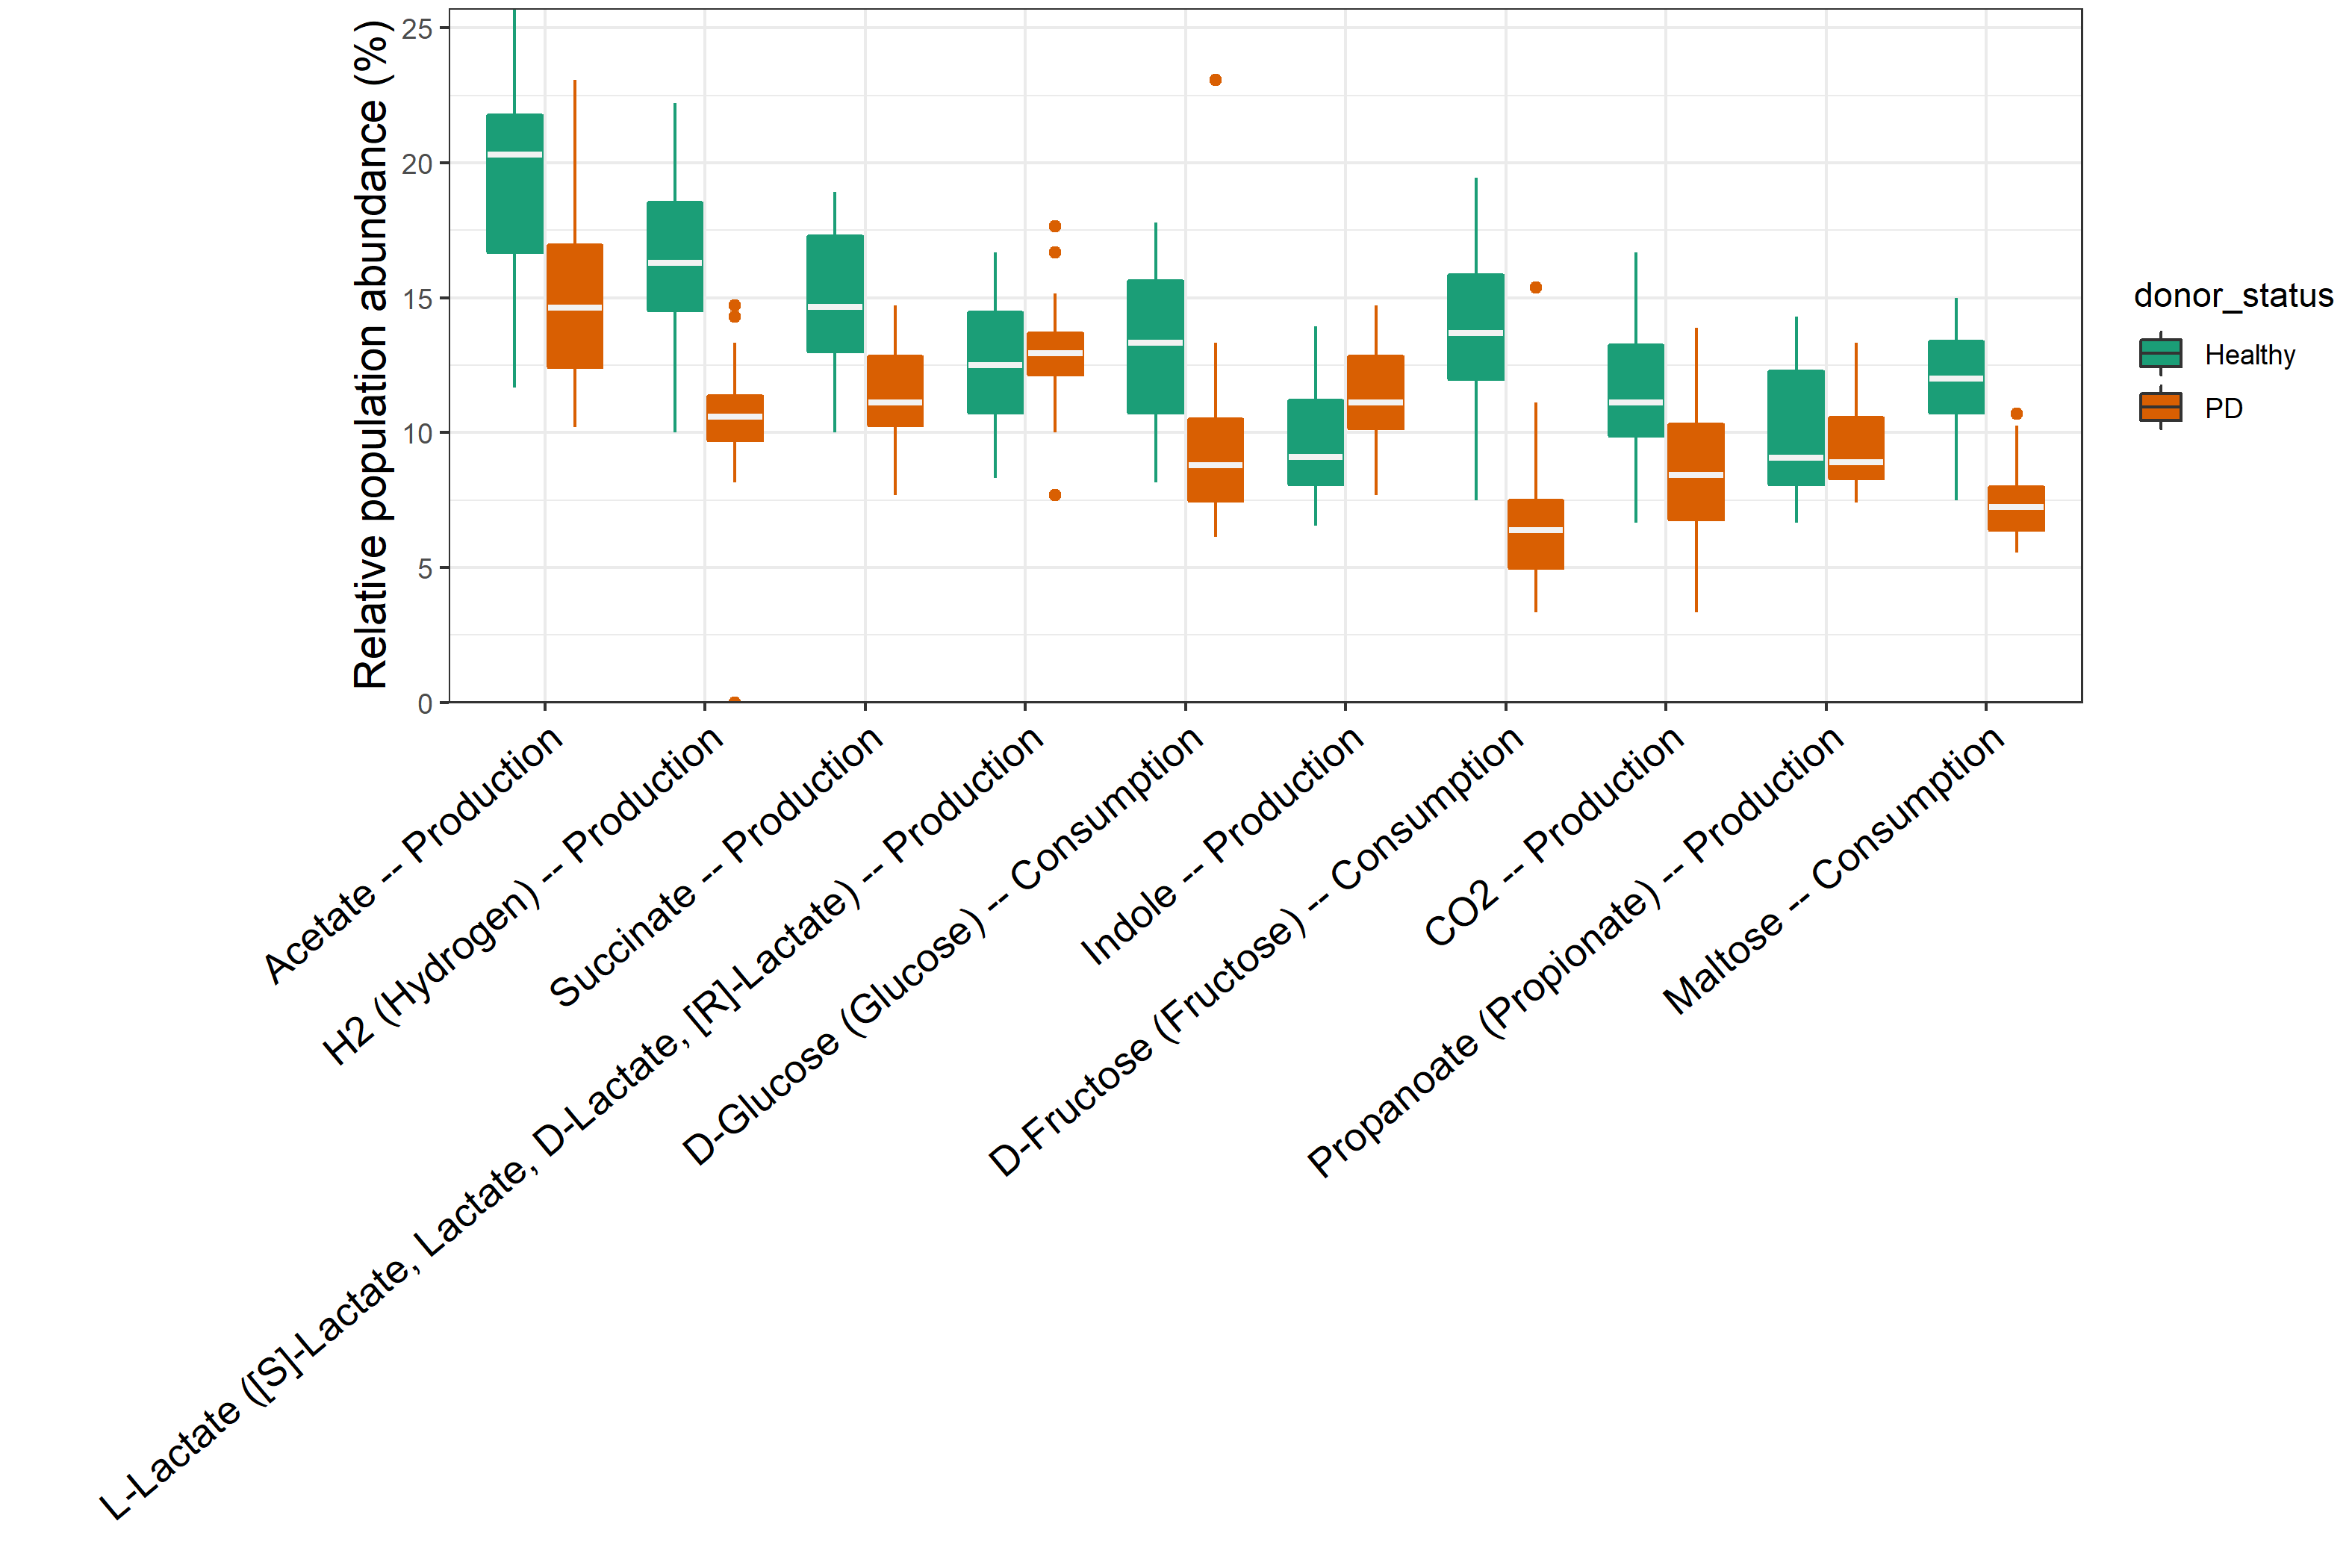
\includegraphics[width=800px]{Images/plot_mouse_NJC19} \end{center}

\hypertarget{notes}{%
\chapter{Notes}\label{notes}}

We show some important things here.

\hypertarget{clone}{%
\section{clone}\label{clone}}

R6 class has a special copy mechanism which is different from S3 and S4.
If you want to copy an object completely, you should use the function clone() instead of direct assignment.

\begin{Shaded}
\begin{Highlighting}[]
\CommentTok{\# use clone to copy completely}
\NormalTok{t1 }\OtherTok{\textless{}{-}} \FunctionTok{clone}\NormalTok{(dataset)}
\NormalTok{t2 }\OtherTok{\textless{}{-}} \FunctionTok{clone}\NormalTok{(t1)}
\NormalTok{t2}\SpecialCharTok{$}\NormalTok{sample\_table }\OtherTok{\textless{}{-}} \ConstantTok{NULL}
\FunctionTok{identical}\NormalTok{(t2, t1)}
\end{Highlighting}
\end{Shaded}

\begin{verbatim}
## [1] FALSE
\end{verbatim}

\begin{Shaded}
\begin{Highlighting}[]
\CommentTok{\# this operation is usually unuseful, because changing t2 will also affect t1}
\NormalTok{t2 }\OtherTok{\textless{}{-}}\NormalTok{ t1}
\NormalTok{t2}\SpecialCharTok{$}\NormalTok{sample\_table }\OtherTok{\textless{}{-}} \ConstantTok{NULL}
\FunctionTok{identical}\NormalTok{(t2, t1)}
\end{Highlighting}
\end{Shaded}

\begin{verbatim}
## [1] TRUE
\end{verbatim}

\hypertarget{subset-of-samples}{%
\section{subset of samples}\label{subset-of-samples}}

We donnot provide the special function to filter samples in microtable class, as we think it is redundant.
We recommend user to directly manipulate the sample\_table in microtable object.
For example, if we want to analyze samples from `CW' and `IW', respectively, we can operate like this:

\begin{Shaded}
\begin{Highlighting}[]
\CommentTok{\# remember first clone the full dataset}
\NormalTok{group1 }\OtherTok{\textless{}{-}} \FunctionTok{clone}\NormalTok{(dataset)}
\NormalTok{group1}\SpecialCharTok{$}\NormalTok{sample\_table }\OtherTok{\textless{}{-}} \FunctionTok{subset}\NormalTok{(group1}\SpecialCharTok{$}\NormalTok{sample\_table, Group }\SpecialCharTok{==} \StringTok{"CW"}\NormalTok{)}
\CommentTok{\# this is necessary to make files in group1 corresponding}
\NormalTok{group1}\SpecialCharTok{$}\FunctionTok{tidy\_dataset}\NormalTok{()}

\CommentTok{\# similar with obove operation}
\NormalTok{group2 }\OtherTok{\textless{}{-}} \FunctionTok{clone}\NormalTok{(dataset)}
\NormalTok{group2}\SpecialCharTok{$}\NormalTok{sample\_table }\OtherTok{\textless{}{-}} \FunctionTok{subset}\NormalTok{(group2}\SpecialCharTok{$}\NormalTok{sample\_table, Group }\SpecialCharTok{==} \StringTok{"IW"}\NormalTok{)}
\NormalTok{group2}\SpecialCharTok{$}\FunctionTok{tidy\_dataset}\NormalTok{()}
\CommentTok{\# now we get two microtable objects: group1 for CW and group2 for IW}
\end{Highlighting}
\end{Shaded}

\hypertarget{change-object}{%
\section{change object}\label{change-object}}

All the classes are set public, meaning that you can change, add or remove the objects stored in them as you want.

\begin{Shaded}
\begin{Highlighting}[]
\CommentTok{\# add a matrix you think useful}
\NormalTok{dataset}\SpecialCharTok{$}\NormalTok{my\_matrix }\OtherTok{\textless{}{-}} \FunctionTok{matrix}\NormalTok{(}\DecValTok{1}\NormalTok{, }\AttributeTok{nrow =} \DecValTok{4}\NormalTok{, }\AttributeTok{ncol =} \DecValTok{4}\NormalTok{)}
\CommentTok{\# change the information}
\NormalTok{dataset}\SpecialCharTok{$}\NormalTok{sample\_table }\SpecialCharTok{\%\textless{}\textgreater{}\%}\NormalTok{ .[, }\SpecialCharTok{{-}}\DecValTok{2}\NormalTok{]}
\end{Highlighting}
\end{Shaded}

\hypertarget{group-order}{%
\section{group order}\label{group-order}}

If you want to reorder the groups, assign the factors may be the most simplest way.

\begin{Shaded}
\begin{Highlighting}[]
\FunctionTok{data}\NormalTok{(dataset)}
\NormalTok{t1 }\OtherTok{\textless{}{-}}\NormalTok{ trans\_beta}\SpecialCharTok{$}\FunctionTok{new}\NormalTok{(}\AttributeTok{dataset =}\NormalTok{ dataset, }\AttributeTok{group =} \StringTok{"Group"}\NormalTok{, }\AttributeTok{measure =} \StringTok{"bray"}\NormalTok{)}
\end{Highlighting}
\end{Shaded}

\begin{verbatim}
## Please also cite the original paper: An et al. (2019). Soil bacterial community structure in Chinese wetlands. Geoderma, 337, 290-299.
\end{verbatim}

\begin{Shaded}
\begin{Highlighting}[]
\NormalTok{t1}\SpecialCharTok{$}\FunctionTok{cal\_ordination}\NormalTok{(}\AttributeTok{ordination =} \StringTok{"PCoA"}\NormalTok{)}
\end{Highlighting}
\end{Shaded}

\begin{verbatim}
## The ordination result is stored in object$res_ordination ...
\end{verbatim}

\begin{Shaded}
\begin{Highlighting}[]
\NormalTok{t1}\SpecialCharTok{$}\FunctionTok{plot\_ordination}\NormalTok{(}\AttributeTok{plot\_color =} \StringTok{"Group"}\NormalTok{, }\AttributeTok{plot\_shape =} \StringTok{"Group"}\NormalTok{, }\AttributeTok{plot\_group\_ellipse =} \ConstantTok{TRUE}\NormalTok{)}
\end{Highlighting}
\end{Shaded}

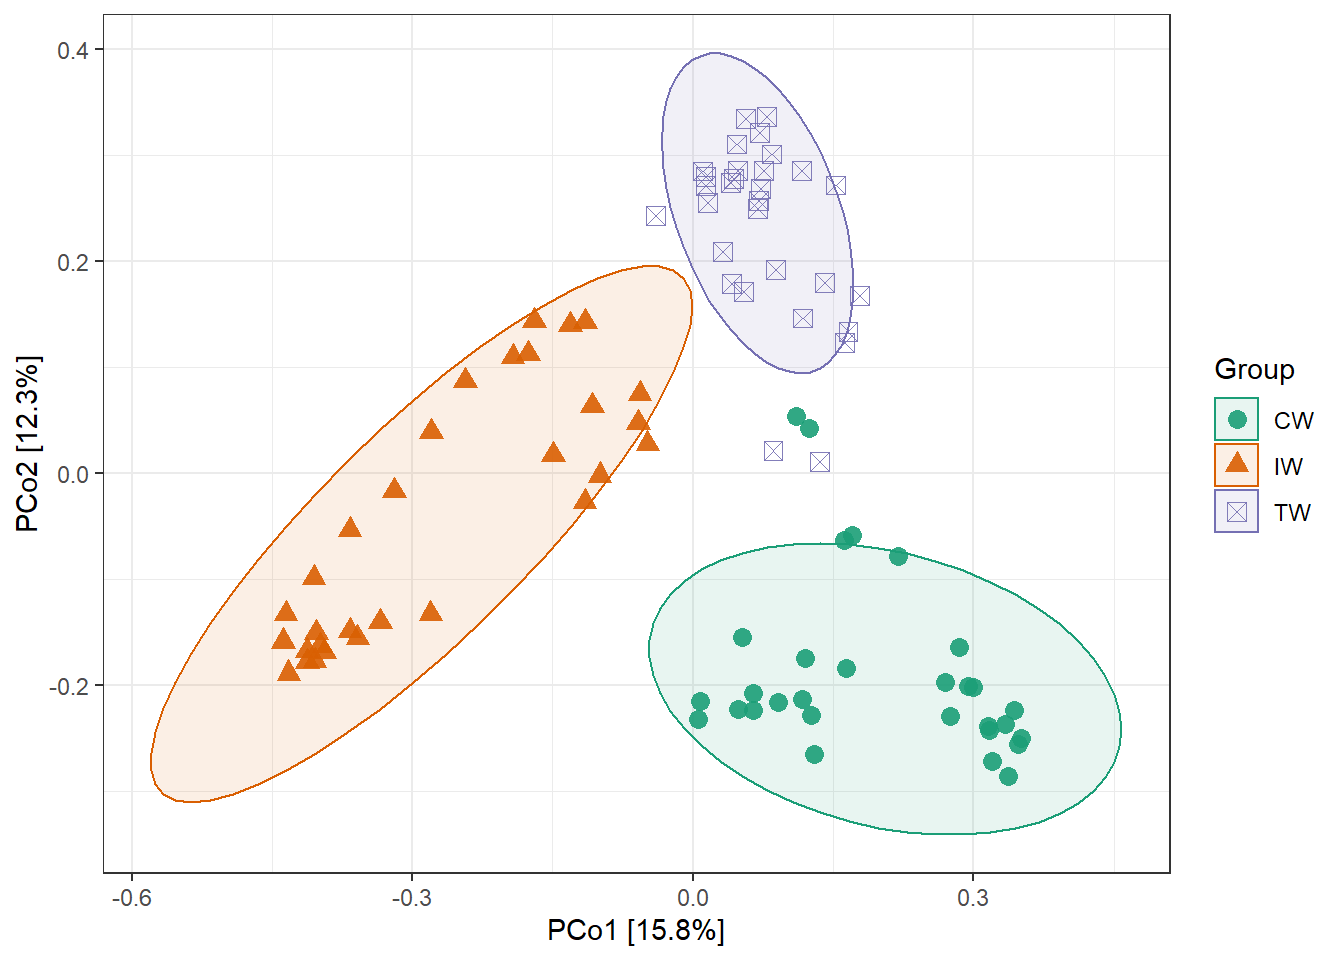
\includegraphics{microeco-tutorial_files/figure-latex/unnamed-chunk-184-1.pdf}

Then we assign factors to the `Group' in sample\_table of dataset.
We can find the changed group order in the legend and colors in the plot.

\begin{Shaded}
\begin{Highlighting}[]
\NormalTok{dataset}\SpecialCharTok{$}\NormalTok{sample\_table}\SpecialCharTok{$}\NormalTok{Group }\SpecialCharTok{\%\textless{}\textgreater{}\%} \FunctionTok{factor}\NormalTok{(., }\AttributeTok{levels =} \FunctionTok{c}\NormalTok{(}\StringTok{"IW"}\NormalTok{, }\StringTok{"TW"}\NormalTok{, }\StringTok{"CW"}\NormalTok{))}
\FunctionTok{str}\NormalTok{(dataset}\SpecialCharTok{$}\NormalTok{sample\_table)}
\end{Highlighting}
\end{Shaded}

\begin{verbatim}
## 'data.frame':    90 obs. of  4 variables:
##  $ SampleID: chr  "S1" "S2" "S3" "S4" ...
##  $ Group   : Factor w/ 3 levels "IW","TW","CW": 1 1 1 1 1 1 1 1 1 1 ...
##  $ Type    : chr  "NE" "NE" "NE" "NE" ...
##  $ Saline  : chr  "Non-saline soil" "Non-saline soil" "Non-saline soil" "Non-saline soil" ...
\end{verbatim}

\begin{Shaded}
\begin{Highlighting}[]
\NormalTok{t1 }\OtherTok{\textless{}{-}}\NormalTok{ trans\_beta}\SpecialCharTok{$}\FunctionTok{new}\NormalTok{(}\AttributeTok{dataset =}\NormalTok{ dataset, }\AttributeTok{group =} \StringTok{"Group"}\NormalTok{, }\AttributeTok{measure =} \StringTok{"bray"}\NormalTok{)}
\end{Highlighting}
\end{Shaded}

\begin{verbatim}
## Please also cite the original paper: An et al. (2019). Soil bacterial community structure in Chinese wetlands. Geoderma, 337, 290-299.
\end{verbatim}

\begin{Shaded}
\begin{Highlighting}[]
\NormalTok{t1}\SpecialCharTok{$}\FunctionTok{cal\_ordination}\NormalTok{(}\AttributeTok{ordination =} \StringTok{"PCoA"}\NormalTok{)}
\end{Highlighting}
\end{Shaded}

\begin{verbatim}
## The ordination result is stored in object$res_ordination ...
\end{verbatim}

\begin{Shaded}
\begin{Highlighting}[]
\NormalTok{t1}\SpecialCharTok{$}\FunctionTok{plot\_ordination}\NormalTok{(}\AttributeTok{plot\_color =} \StringTok{"Group"}\NormalTok{, }\AttributeTok{plot\_shape =} \StringTok{"Group"}\NormalTok{, }\AttributeTok{plot\_group\_ellipse =} \ConstantTok{TRUE}\NormalTok{)}
\end{Highlighting}
\end{Shaded}

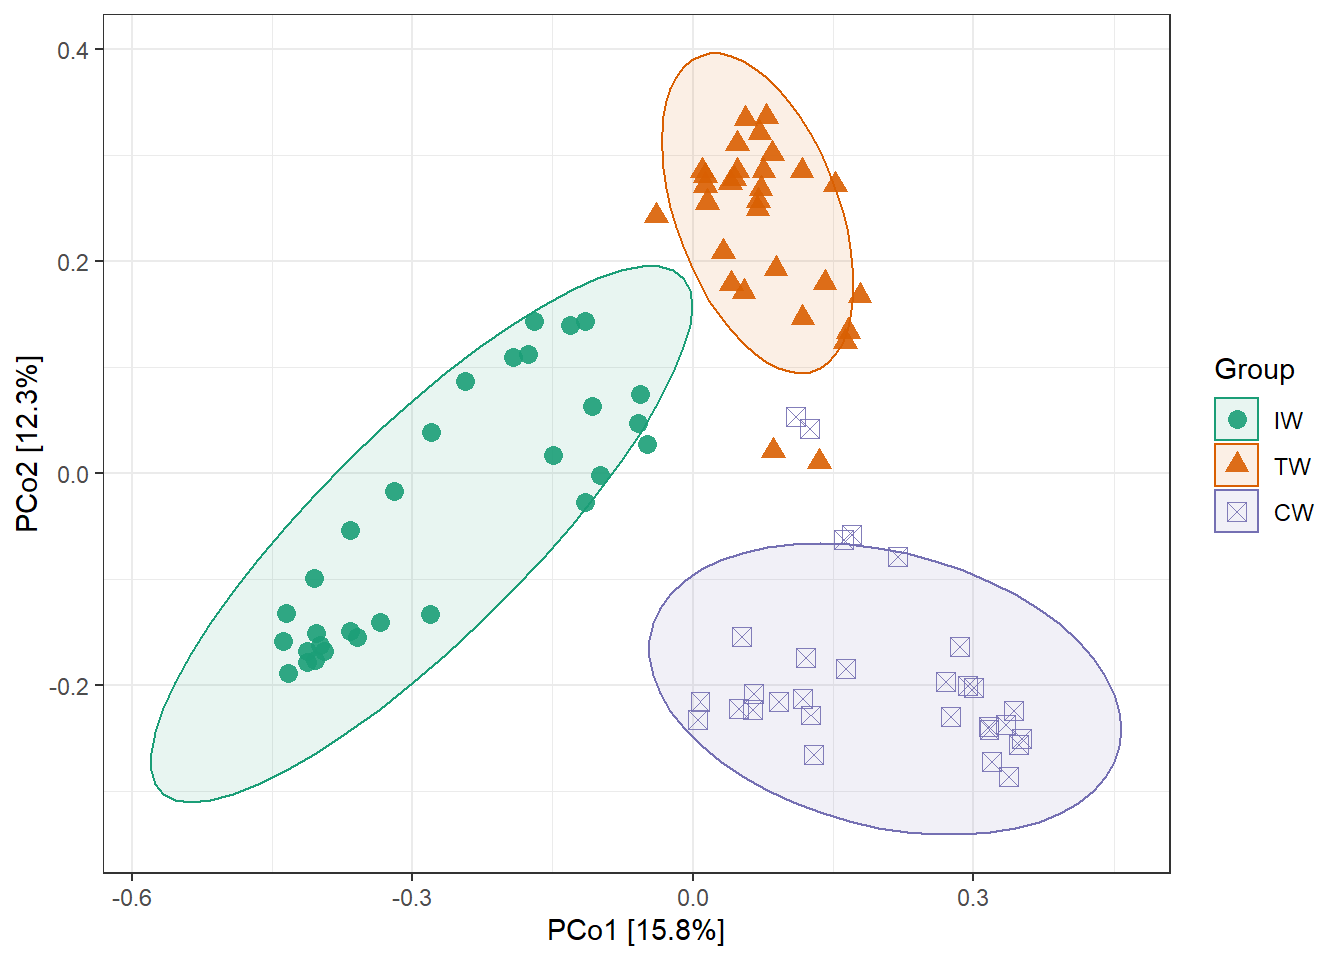
\includegraphics{microeco-tutorial_files/figure-latex/unnamed-chunk-185-1.pdf}

\hypertarget{add-layers-to-plot}{%
\section{add layers to plot}\label{add-layers-to-plot}}

Most of the plots are generated by applying the ggplot2 package.
The important parameters in the plotting functions are configured according to our experience.
If the inner parameters can not enough, the user can add the layers to the plot like the following operation or
make the plot using the data (generally data.frame class) stored in the object.

\begin{Shaded}
\begin{Highlighting}[]
\CommentTok{\# The groupmean parameter can be used to obtain the group{-}mean barplot.}
\NormalTok{t1 }\OtherTok{\textless{}{-}}\NormalTok{ trans\_abund}\SpecialCharTok{$}\FunctionTok{new}\NormalTok{(}\AttributeTok{dataset =}\NormalTok{ dataset, }\AttributeTok{taxrank =} \StringTok{"Phylum"}\NormalTok{, }\AttributeTok{ntaxa =} \DecValTok{10}\NormalTok{, }\AttributeTok{groupmean =} \StringTok{"Group"}\NormalTok{)}
\NormalTok{g1 }\OtherTok{\textless{}{-}}\NormalTok{ t1}\SpecialCharTok{$}\FunctionTok{plot\_bar}\NormalTok{(}\AttributeTok{others\_color =} \StringTok{"grey70"}\NormalTok{, }\AttributeTok{legend\_text\_italic =} \ConstantTok{FALSE}\NormalTok{)}
\NormalTok{g1 }\SpecialCharTok{+} \FunctionTok{theme\_classic}\NormalTok{() }\SpecialCharTok{+} \FunctionTok{theme}\NormalTok{(}\AttributeTok{axis.title.y =} \FunctionTok{element\_text}\NormalTok{(}\AttributeTok{size =} \DecValTok{18}\NormalTok{))}
\end{Highlighting}
\end{Shaded}

\begin{center}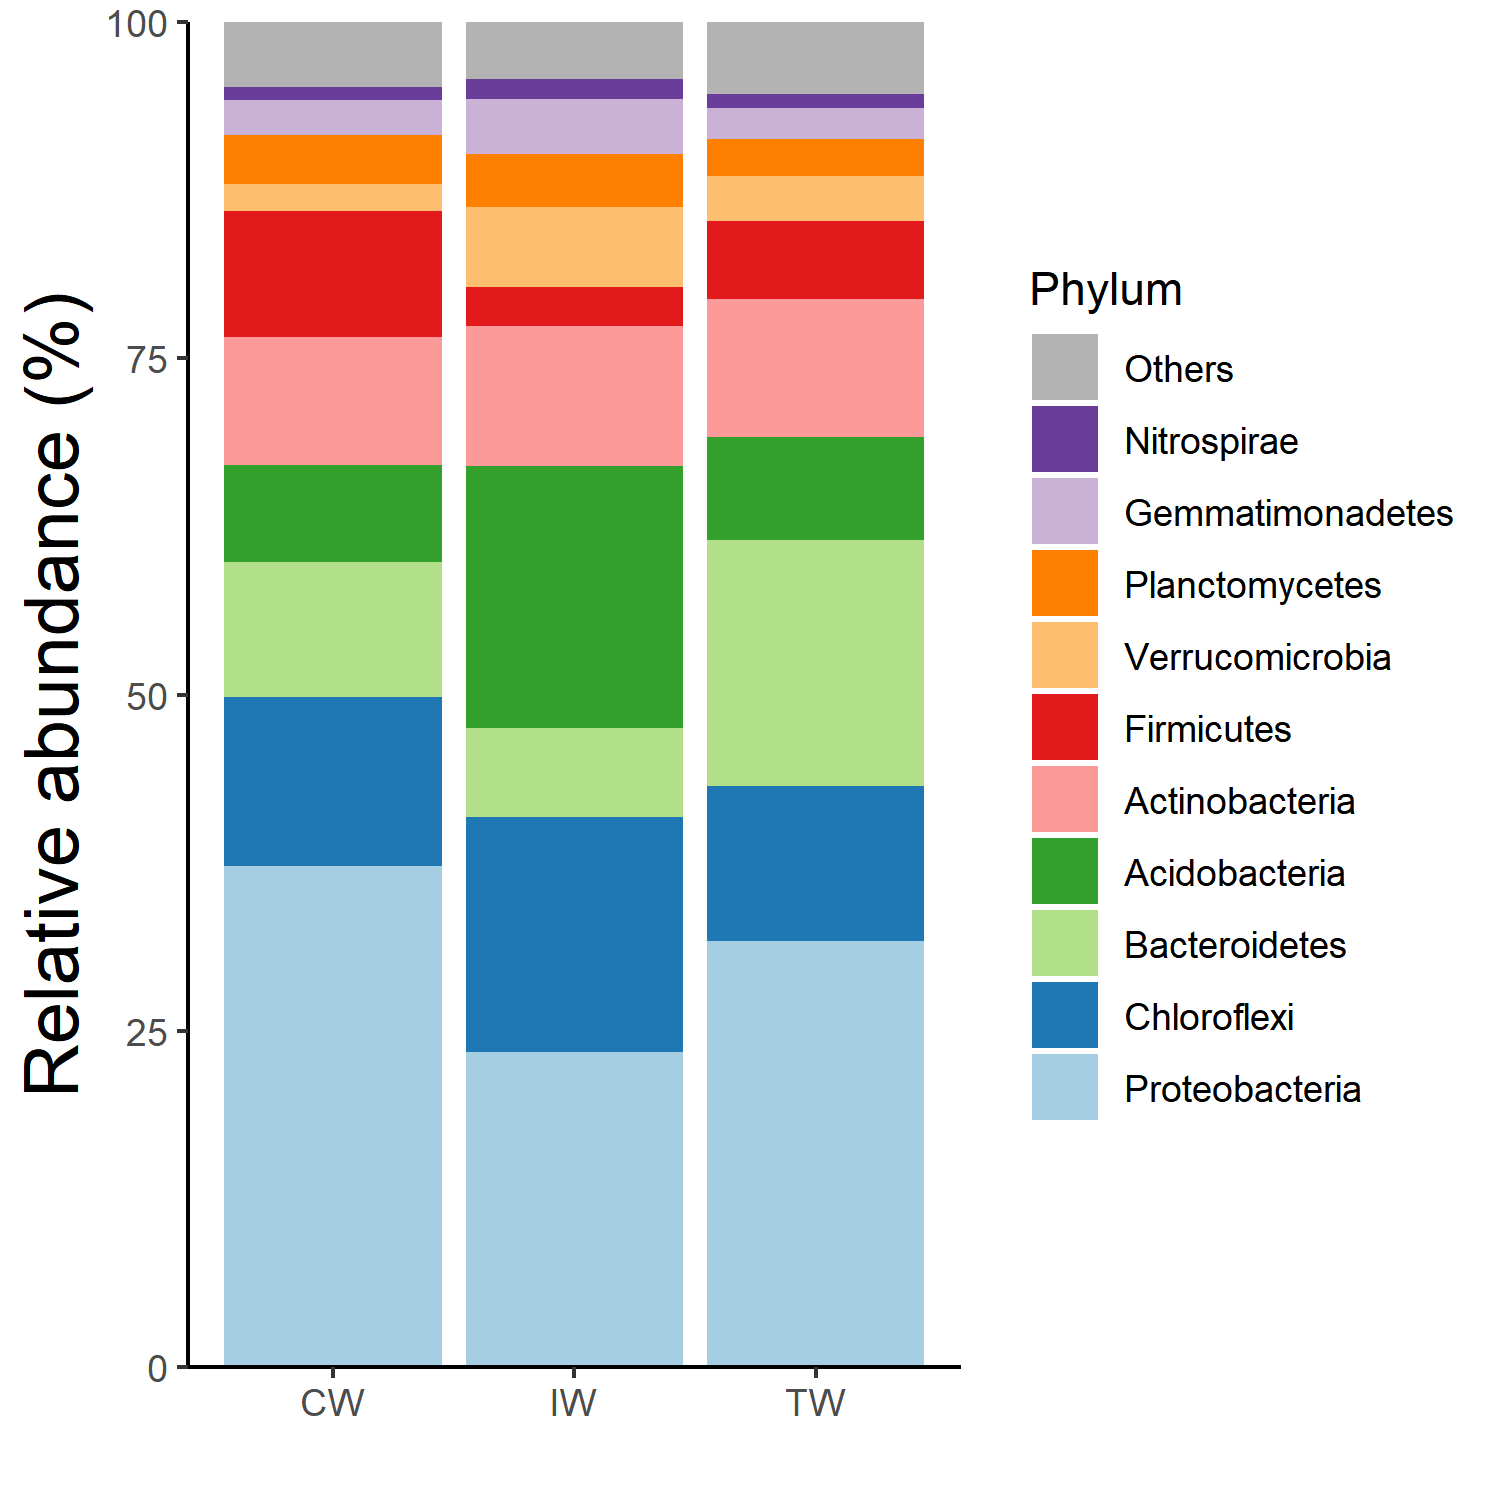
\includegraphics[width=400px]{Images/plot_bar_mean_classic} \end{center}

\hypertarget{mecodev-package}{%
\chapter{mecodev package}\label{mecodev-package}}

The mecodev package (\url{https://github.com/ChiLiubio/mecodev/}) is designed to develop more classes for data analysis based on the microeco package.

\hypertarget{trans_rarefy}{%
\section{trans\_rarefy}\label{trans_rarefy}}

The class trans\_rarefy in mecodev package can be used for the rarefaction and the following plotting to see whether
the sequencing depth is enough to cover all the so-called species in the microbial community.

\begin{Shaded}
\begin{Highlighting}[]
\FunctionTok{library}\NormalTok{(microeco)}
\FunctionTok{library}\NormalTok{(mecodev)}
\FunctionTok{data}\NormalTok{(sample\_info\_16S)}
\FunctionTok{data}\NormalTok{(otu\_table\_16S)}
\CommentTok{\# set.seed is used to fix the random number generation to make the results repeatable}
\FunctionTok{set.seed}\NormalTok{(}\DecValTok{123}\NormalTok{)}
\NormalTok{dataset }\OtherTok{\textless{}{-}}\NormalTok{ microtable}\SpecialCharTok{$}\FunctionTok{new}\NormalTok{(}\AttributeTok{sample\_table =}\NormalTok{ sample\_info\_16S, }\AttributeTok{otu\_table =}\NormalTok{ otu\_table\_16S)}
\NormalTok{dataset}\SpecialCharTok{$}\FunctionTok{tidy\_dataset}\NormalTok{()}
\CommentTok{\# trans\_rarefy class}
\NormalTok{t1 }\OtherTok{\textless{}{-}}\NormalTok{ trans\_rarefy}\SpecialCharTok{$}\FunctionTok{new}\NormalTok{(dataset, }\AttributeTok{alphadiv =} \StringTok{"Shannon"}\NormalTok{, }\AttributeTok{depth =} \FunctionTok{c}\NormalTok{(}\DecValTok{0}\NormalTok{, }\DecValTok{10}\NormalTok{, }\DecValTok{50}\NormalTok{, }\DecValTok{500}\NormalTok{, }\DecValTok{2000}\NormalTok{, }\DecValTok{4000}\NormalTok{, }\DecValTok{6000}\NormalTok{, }\DecValTok{8000}\NormalTok{))}
\NormalTok{t1}\SpecialCharTok{$}\FunctionTok{plot\_rarefy}\NormalTok{(}\AttributeTok{color\_values =} \FunctionTok{rep}\NormalTok{(}\StringTok{"grey"}\NormalTok{, }\DecValTok{100}\NormalTok{), }\AttributeTok{show\_point =} \ConstantTok{TRUE}\NormalTok{, }\AttributeTok{add\_fitting =} \ConstantTok{FALSE}\NormalTok{, }\AttributeTok{show\_legend =} \ConstantTok{FALSE}\NormalTok{)}
\end{Highlighting}
\end{Shaded}

\begin{center}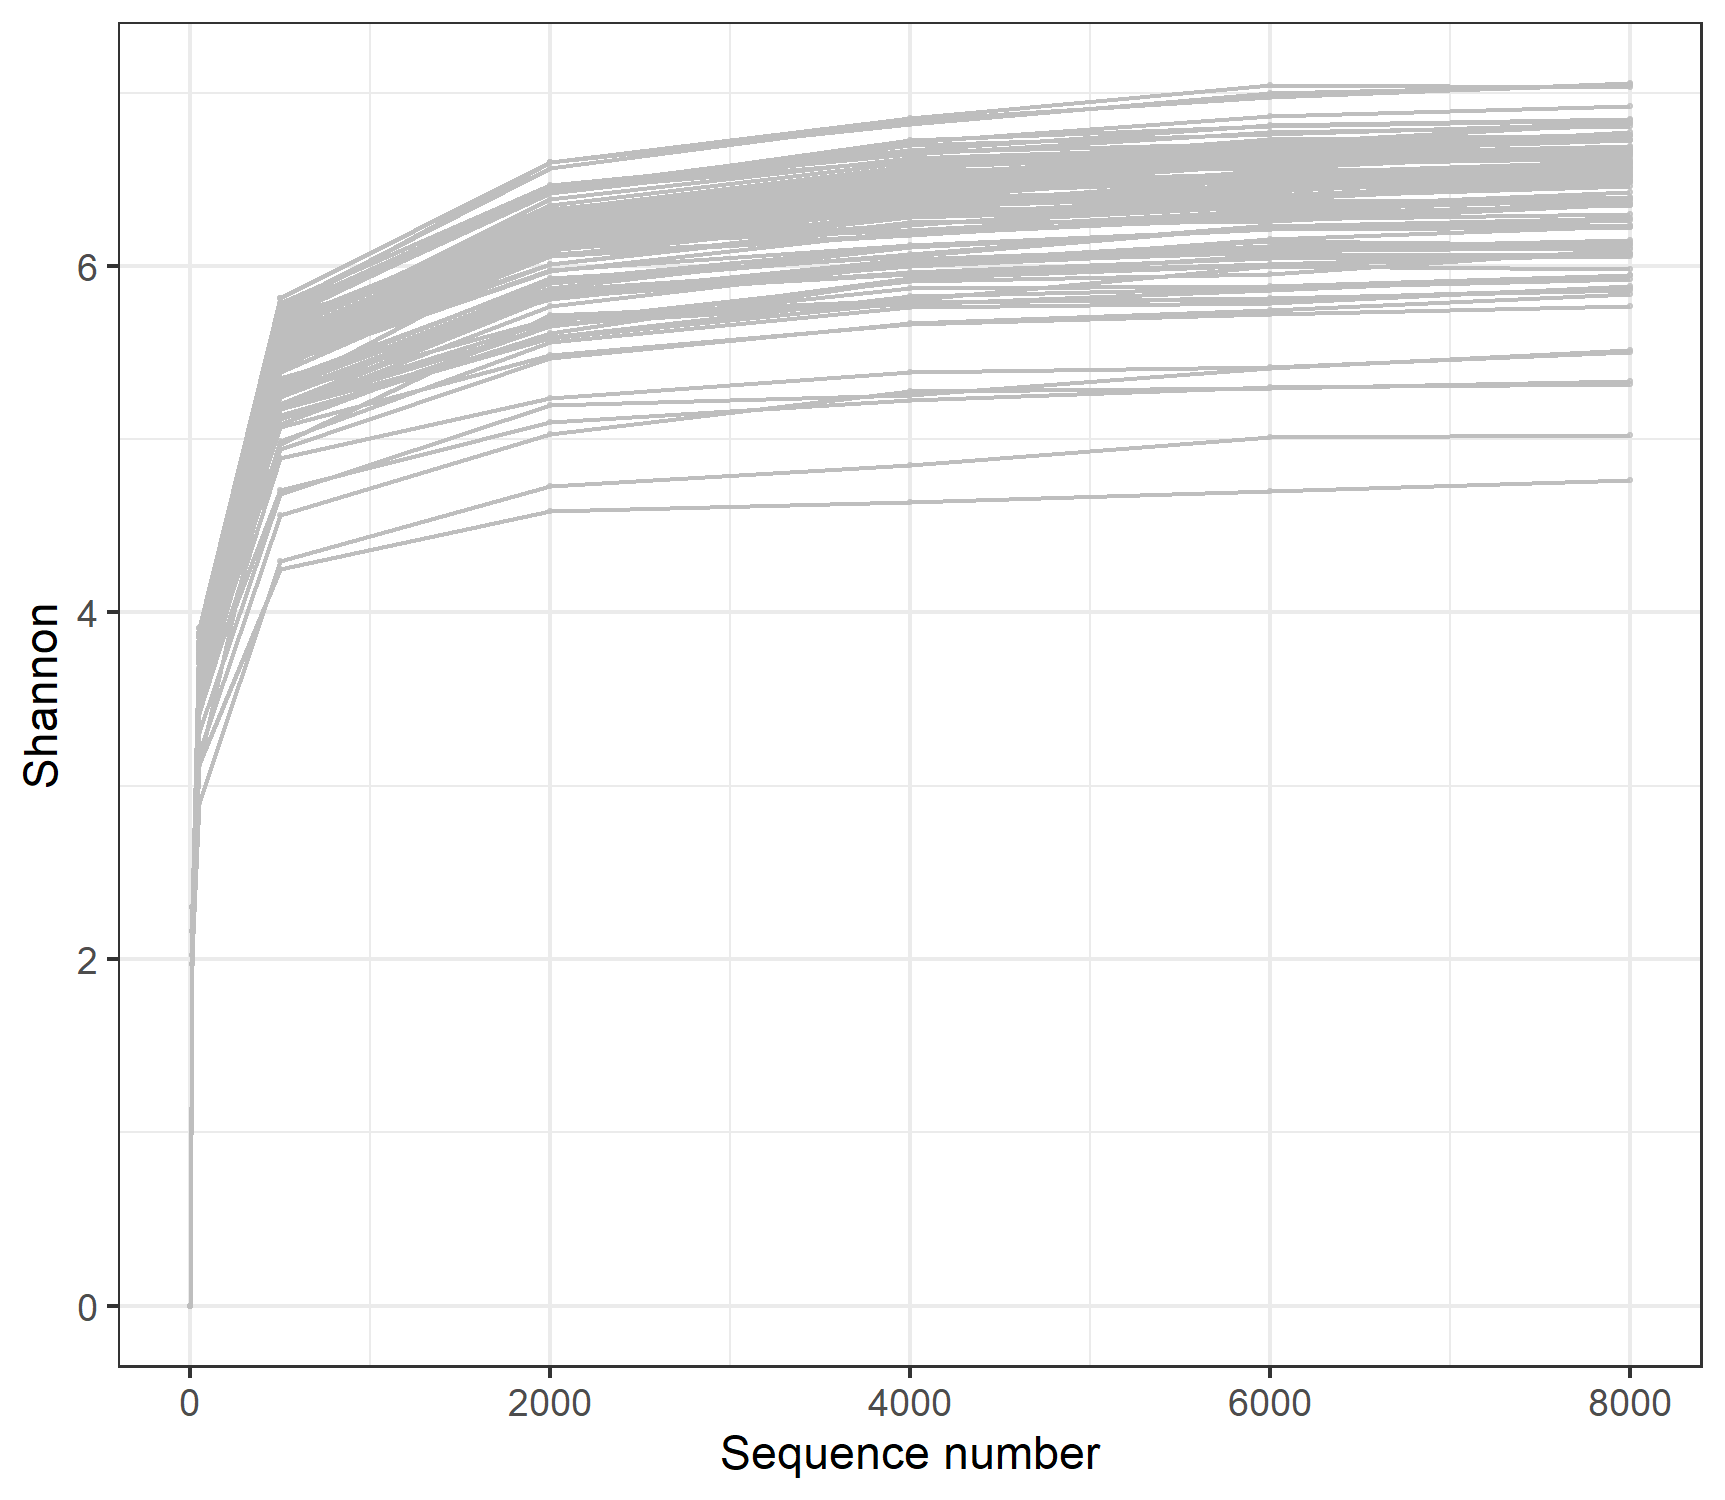
\includegraphics[width=550px]{Images/plot_trans_rarefy} \end{center}

\hypertarget{trans_convert}{%
\section{trans\_convert}\label{trans_convert}}

The class trans\_convert provide several data transformation approaches for the microtable object.
The output will also be a microtable object.

\begin{Shaded}
\begin{Highlighting}[]
\FunctionTok{data}\NormalTok{(dataset)}
\NormalTok{test1 }\OtherTok{\textless{}{-}}\NormalTok{ trans\_convert}\SpecialCharTok{$}\FunctionTok{new}\NormalTok{(}\AttributeTok{dataset =}\NormalTok{ dataset)}
\NormalTok{test2 }\OtherTok{\textless{}{-}}\NormalTok{ test1}\SpecialCharTok{$}\FunctionTok{convert}\NormalTok{(}\AttributeTok{method =} \StringTok{"log"}\NormalTok{)}
\CommentTok{\# returned test2 is another microtable object}
\end{Highlighting}
\end{Shaded}

\hypertarget{trans_netchord}{%
\section{trans\_netchord}\label{trans_netchord}}

The class trans\_netchord is developed to sum and plot the links number from one taxa to another or in the same taxa in the network.
The input dataset must be a trans\_network object.
Creating the trans\_netchord object can sum the links (edge) number from one taxa to another or in the same taxa.
The function plot\_sum\_links() is used to show the result from the function cal\_sum\_links().
This is very useful to fast see how many nodes are connected between different taxa or within one taxa.
In terms of ``Phylum'' level in the tutorial,
the function cal\_sum\_links() sum the linkages number from one Phylum to another Phylum or the linkages in the same Phylum.
So the numbers along the outside of the circular plot represent how many edges or linkages are related with the Phylum.
For example, in terms of Proteobacteria,
there are roughly total 900 edges associated with the OTUs in Proteobacteria,
in which roughly 200 edges connect both OTUs in Proteobacteria and roughly 150 edges connect the OTUs from Proteobacteria with the OTUs from Chloroflexi.

\begin{Shaded}
\begin{Highlighting}[]
\CommentTok{\# Let\textquotesingle{}s first create a network}
\FunctionTok{data}\NormalTok{(sample\_info\_16S)}
\FunctionTok{data}\NormalTok{(otu\_table\_16S)}
\FunctionTok{data}\NormalTok{(taxonomy\_table\_16S)}
\NormalTok{dataset }\OtherTok{\textless{}{-}}\NormalTok{ microtable}\SpecialCharTok{$}\FunctionTok{new}\NormalTok{(}\AttributeTok{sample\_table =}\NormalTok{ sample\_info\_16S, }\AttributeTok{otu\_table =}\NormalTok{ otu\_table\_16S, }\AttributeTok{tax\_table =}\NormalTok{ taxonomy\_table\_16S)}
\NormalTok{dataset}\SpecialCharTok{$}\FunctionTok{tidy\_dataset}\NormalTok{()}
\NormalTok{t1 }\OtherTok{\textless{}{-}}\NormalTok{ trans\_network}\SpecialCharTok{$}\FunctionTok{new}\NormalTok{(}\AttributeTok{dataset =}\NormalTok{ dataset, }\AttributeTok{cal\_cor =} \StringTok{"WGCNA"}\NormalTok{, }\AttributeTok{taxa\_level =} \StringTok{"OTU"}\NormalTok{, }\AttributeTok{filter\_thres =} \FloatTok{0.0001}\NormalTok{, }\AttributeTok{cor\_method =} \StringTok{"spearman"}\NormalTok{)}
\NormalTok{t1}\SpecialCharTok{$}\FunctionTok{cal\_network}\NormalTok{(}\AttributeTok{p\_thres =} \FloatTok{0.01}\NormalTok{, }\AttributeTok{COR\_cut =} \FloatTok{0.7}\NormalTok{)}
\CommentTok{\# trans\_netchord}
\NormalTok{test1 }\OtherTok{\textless{}{-}}\NormalTok{ trans\_netchord}\SpecialCharTok{$}\FunctionTok{new}\NormalTok{(}\AttributeTok{dataset =}\NormalTok{ t1, }\AttributeTok{taxa\_level =} \StringTok{"Phylum"}\NormalTok{)}
\CommentTok{\# require chorddiag package (https://github.com/mattflor/chorddiag)}
\NormalTok{test1}\SpecialCharTok{$}\FunctionTok{plot\_sum\_links}\NormalTok{(}\AttributeTok{plot\_pos =} \ConstantTok{TRUE}\NormalTok{, }\AttributeTok{plot\_num =} \DecValTok{10}\NormalTok{)}
\end{Highlighting}
\end{Shaded}

\begin{center}\includegraphics[width=700px]{Images/plot_sum_links} \end{center}

\hypertarget{trans_ts}{%
\section{trans\_ts}\label{trans_ts}}

The class trans\_ts is designed for the time series data analysis.
A commonly used approach for modeling microbial ecology for time series data is the generalized Lotka-Volterra (gLV) model, the classical predator-prey systems.
gLV models are based on ordinary differential equations that model the logistic growth of species;
naturally capture predator-prey, amensalistic, and competitive interactions; and have been applied to study dynamics of microbial ecosystems.
More importantly, from a practical perspective, gLV models have been used for a range of applications including identifying potential probiotics
against pathogens, forecasting changes in microbial density, characterizing important community members (e.g., keystone species),
and analyzing community stability (see \citep{Li_expectation_2019} and the references therein).
Currently, the biomass estimation and biological interaction prediction approaches are implemented based on the beem package \citep{Li_expectation_2019}.

\begin{Shaded}
\begin{Highlighting}[]
\CommentTok{\# R package beem should be first installed; see https://github.com/ChiLiubio/mecodev for installation steps}
\FunctionTok{library}\NormalTok{(mecodev)}
\CommentTok{\# load the example data in mecodev package; the input must be a microtable object}
\CommentTok{\# There are several strict requirements on the sample\_table; see the document of the class.}
\FunctionTok{data}\NormalTok{(}\StringTok{"gut\_microb\_ts"}\NormalTok{)}
\CommentTok{\# generally, using filter\_thres to filter the taxa with low abundance is crutial}
\CommentTok{\# there are only 22 taxa in the example data, we use 0}
\NormalTok{t1 }\OtherTok{\textless{}{-}}\NormalTok{ trans\_ts}\SpecialCharTok{$}\FunctionTok{new}\NormalTok{(}\AttributeTok{dataset =}\NormalTok{ gut\_microb\_ts, }\AttributeTok{filter\_thres =} \DecValTok{0}\NormalTok{)}
\CommentTok{\# we use minimal 50 times for iteration}
\NormalTok{t1}\SpecialCharTok{$}\FunctionTok{cal\_biomass}\NormalTok{(}\AttributeTok{min\_iter =} \DecValTok{50}\NormalTok{)}
\CommentTok{\# return t1$res\_biomass and t1$res\_param}
\CommentTok{\# generate the inferred biological network}
\NormalTok{t1}\SpecialCharTok{$}\FunctionTok{cal\_network}\NormalTok{()}
\CommentTok{\# Now let\textquotesingle{}s use trans\_network class to add the modules}
\FunctionTok{library}\NormalTok{(microeco)}
\NormalTok{t2 }\OtherTok{\textless{}{-}}\NormalTok{ trans\_network}\SpecialCharTok{$}\FunctionTok{new}\NormalTok{(}\AttributeTok{dataset =}\NormalTok{ gut\_microb\_ts, }\AttributeTok{cal\_cor =} \ConstantTok{NA}\NormalTok{)}
\NormalTok{t2}\SpecialCharTok{$}\NormalTok{res\_network }\OtherTok{\textless{}{-}}\NormalTok{ t1}\SpecialCharTok{$}\NormalTok{res\_network}
\CommentTok{\# use cluster\_optimal; as the default cluster\_fast\_greedy can not be used for the directed network}
\NormalTok{t2}\SpecialCharTok{$}\FunctionTok{cal\_module}\NormalTok{(}\AttributeTok{method =} \StringTok{"cluster\_optimal"}\NormalTok{)}
\FunctionTok{plot}\NormalTok{(t2}\SpecialCharTok{$}\NormalTok{res\_network)}
\end{Highlighting}
\end{Shaded}

\hypertarget{trans_gamma}{%
\section{trans\_gamma}\label{trans_gamma}}

The class trans\_gamma is developed to explore the relationship between gamma diversity and beta diversity
based on the methods from biogeographic studies\citep{Zhang_Local_2020}.
Currently, the contents include the observed beta-gamma diversity relationship, simulated beta-gamma diversity relationship and the following plotting.
If the observed gamma diversity and beta diversity are significantly correlated,
species pool at regional scale (or maybe your defined scale, e.g., different treatments in the lab) can have large effect on the beta diversity.
Thus, species pool should be first considered to explain beta diversity patterns.
This class also provide simulation function to explore the relation between gamma diversity and beta diversity in the absence of any process
other than random sampling based on the species log-normal distribution.
We use the wetland data to show the observed beta-gamma diversity relationship.

\begin{Shaded}
\begin{Highlighting}[]
\FunctionTok{library}\NormalTok{(microeco)}
\FunctionTok{library}\NormalTok{(mecodev)}
\CommentTok{\# load the example data}
\FunctionTok{data}\NormalTok{(sample\_info\_16S)}
\FunctionTok{data}\NormalTok{(otu\_table\_16S)}
\NormalTok{test }\OtherTok{\textless{}{-}}\NormalTok{ microtable}\SpecialCharTok{$}\FunctionTok{new}\NormalTok{(}\AttributeTok{sample\_table =}\NormalTok{ sample\_info\_16S, }\AttributeTok{otu\_table =}\NormalTok{ otu\_table\_16S)}
\NormalTok{test}\SpecialCharTok{$}\FunctionTok{tidy\_dataset}\NormalTok{()}
\NormalTok{test}\SpecialCharTok{$}\FunctionTok{rarefy\_samples}\NormalTok{(}\AttributeTok{sample.size =} \DecValTok{10000}\NormalTok{)}
\CommentTok{\# then create trans\_gamma object}
\NormalTok{test1 }\OtherTok{\textless{}{-}}\NormalTok{ trans\_gamma}\SpecialCharTok{$}\FunctionTok{new}\NormalTok{(}\AttributeTok{dataset =}\NormalTok{ test, }\AttributeTok{group =} \StringTok{"Type"}\NormalTok{, }\AttributeTok{method =} \StringTok{"bray"}\NormalTok{)}
\NormalTok{test1}\SpecialCharTok{$}\FunctionTok{cal\_observed}\NormalTok{(}\AttributeTok{sample\_size =} \ConstantTok{NULL}\NormalTok{)}
\NormalTok{test1}\SpecialCharTok{$}\NormalTok{res\_observed}
\CommentTok{\# use Spearman correlation}
\NormalTok{test1}\SpecialCharTok{$}\FunctionTok{plot\_observed}\NormalTok{(}\AttributeTok{cor\_method =} \StringTok{"spearman"}\NormalTok{)}
\end{Highlighting}
\end{Shaded}

\begin{center}\includegraphics[width=550px]{Images/plot_gamma_obs} \end{center}

Let's simulate the relation between gamma diversity and beta diversity in the absence of any process
other than random sampling based on the species log-normal distribution.

\begin{Shaded}
\begin{Highlighting}[]
\CommentTok{\# if you only run the simulation, dataset parameter is not necessary}
\NormalTok{test1 }\OtherTok{\textless{}{-}}\NormalTok{ trans\_gamma}\SpecialCharTok{$}\FunctionTok{new}\NormalTok{(}\AttributeTok{method =} \StringTok{"bray"}\NormalTok{)}
\CommentTok{\# use individul numbers at 200, 1000 and 2000, and hypothesize each species pool have 20 samples.}
\NormalTok{test1}\SpecialCharTok{$}\FunctionTok{cal\_simulation}\NormalTok{(}\AttributeTok{ncom =} \DecValTok{20}\NormalTok{, }\AttributeTok{ind\_vect =} \FunctionTok{c}\NormalTok{(}\DecValTok{200}\NormalTok{, }\DecValTok{1000}\NormalTok{, }\DecValTok{2000}\NormalTok{))}
\NormalTok{test1}\SpecialCharTok{$}\FunctionTok{plot\_simulation}\NormalTok{(}\AttributeTok{add\_fitting =} \ConstantTok{FALSE}\NormalTok{)}
\end{Highlighting}
\end{Shaded}

\begin{center}\includegraphics[width=600px]{Images/plot_gamma_simu} \end{center}

\hypertarget{other-examples}{%
\chapter{Other examples}\label{other-examples}}

We encourage users to contribute some unique, special and helpful examples inspired by the microeco, file2meco and mecodev package.

\hypertarget{custom-taxa-order-in-bar-plot}{%
\section{Custom taxa order in bar plot}\label{custom-taxa-order-in-bar-plot}}

Jarrod J. Scott contribute a cool answer to the question that how to use custom taxa and the order in bar plot.
This is a discussion topic in microeco Discussions part. Here is the link (\url{https://github.com/ChiLiubio/microeco/discussions/45}).

\hypertarget{the-importance-of-tidy_taxonomy-function}{%
\section{The importance of tidy\_taxonomy function}\label{the-importance-of-tidy_taxonomy-function}}

The taxonomic classification with standard prefix is very important for some analysis methods,
e.g.~taxonomic abundance plotting and biomarker finding.
The tidy\_taxonomy function in microeco package is designed to make the taxa having standard prefix.
See those Issues for the detailed examples: (\url{https://github.com/ChiLiubio/microeco/issues/32}) and (\url{https://github.com/ChiLiubio/microeco/issues/22}).

\hypertarget{question-of-prefix-in-the-taxa}{%
\section{Question of prefix in the taxa}\label{question-of-prefix-in-the-taxa}}

The prefix of taxa in taxonomic table may affect the following performance of plotting, e.g.~text in legend.
Please see those Issues (\url{https://github.com/ChiLiubio/microeco/issues/32}), (\url{https://github.com/ChiLiubio/microeco/issues/7})
and (\url{https://github.com/ChiLiubio/microeco/issues/15}).

\hypertarget{the-use-of-phylogenetic-tree}{%
\section{The use of phylogenetic tree}\label{the-use-of-phylogenetic-tree}}

One of Issues referred to the basic use of phylogenetic tree in the microeco package (\url{https://github.com/ChiLiubio/microeco/issues/33}).

  \bibliography{book.bib,packages.bib}

\end{document}
